\documentclass[a4paper,12pt]{report}
\usepackage{amsmath}
\usepackage{graphicx}
\usepackage{datetime2}
\usepackage{url}
\usepackage{amsfonts}
\usepackage{longtable}
\usepackage{extarrows} 
\usepackage{makecell}
\usepackage[ngerman,american]{babel}
\usepackage[T1]{fontenc}
\usepackage{placeins}
\usepackage{fancyhdr}
\usepackage{multirow}
\usepackage{tikz}
\usepackage{circuitikz}
\usepackage{physics}
\usepackage{url}
\usepackage{xcolor}
\usepackage[smartEllipses]{markdown}
\usepackage{inconsolata}
\usepackage{listings}
\usepackage{etoolbox}
%\usepackage{mathabx}
\usepackage[linesnumbered, ruled, vlined]{algorithm2e}
\usepackage{setspace}
\usepackage[most,skins]{tcolorbox}
\usepackage{subcaption} 
\usetikzlibrary{positioning,calc}
%\usepackage{draftwatermark}
\usepackage{framed}
%\SetWatermarkText{DRAFT}
%\SetWatermarkScale{5}

\usepackage[left=1in,right=1in,top=1.2in,bottom=1.2in]{geometry}

\newcommand{\tikzmark}[1]{\tikz[overlay,remember picture] \node (#1) [anchor=base] {};}
\newcommand{\snode}[3]{\node [] (#1) at (#2) {$\mathstrut #3$}}
\newcommand{\spath}[2]{\draw[<->] (#1) -- (#2) node [midway, above] () {S}}
\newcommand{\ppath}[2]{\draw[<->] (#1) -- (#2) node [midway, above] () {P}}
 
\fancypagestyle{firstpage}{%
\fancyhf{} % clear all six fields
\renewcommand{\headrulewidth}{0pt}
\renewcommand{\footrulewidth}{0pt}
}
\fancypagestyle{firstcoverpage}{%
\fancyhf{} % clear all six fields
\fancyfoot[C]{\thepage}
\renewcommand{\headrulewidth}{0pt}
\renewcommand{\footrulewidth}{0pt}
}
\fancypagestyle{followingpage}{%
\fancyhf{} % clear all six fields
\fancyhead[LE,RO]{\nouppercase{\rightmark}}
\fancyhead[LO,RE]{\textbf{\thepage}}
\renewcommand{\headrulewidth}{0.7pt}
\renewcommand{\footrulewidth}{0pt}
}
\setlength{\headheight}{15pt}
\pagestyle{followingpage}
 

%\documentclass[aip,reprint]{revtex4-1}

\newcommand{\ovl}{\overline}
\newcommand{\unl}{\underline}
\newcommand{\sovl}[1]{\overline{#1}} % \smash{#1}\vphantom{a}}}
\newcommand{\sunl}[1]{\underline{#1}} %\smash{#1}\vphantom{a}}}
\newcommand{\oli}{\overline{i}}
\newcommand{\olj}{\overline{j}}
\newcommand{\olk}{\overline{k}}
\newcommand{\oll}{\overline{l}}
\newcommand{\ola}{\overline{a}}
\newcommand{\olb}{\overline{b}}
\newcommand{\olc}{\overline{c}}
\newcommand{\old}{\overline{d}}

\newcommand{\ooli}{\overline{i}}
\newcommand{\oolj}{\overline{j}}
\newcommand{\oolk}{\overline{k}}
\newcommand{\ooll}{\overline{l}}
\newcommand{\oola}{\overline{a}}
\newcommand{\oolb}{\overline{b}}
\newcommand{\oolc}{\overline{c}}
\newcommand{\oold}{\overline{d}}

\newcommand{\ool}[1]{\overline{#1}}

\newcommand{\eps}{\epsilon}

\newcommand{\olI}{\overline{I}}
\newcommand{\olJ}{\overline{J}}
\newcommand{\olK}{\overline{K}}
\newcommand{\olL}{\overline{L}}
\newcommand{\olA}{\overline{A}}
\newcommand{\olB}{\overline{B}}
\newcommand{\olC}{\overline{C}}
\newcommand{\olD}{\overline{D}}

\newcommand{\doti}{\hat{i}}
\newcommand{\dotj}{\hat{j}}
\newcommand{\dotk}{\hat{k}}
\newcommand{\dotl}{\hat{l}}

\newcommand{\dota}{\hat{a}}
\newcommand{\dotb}{\hat{b}}
\newcommand{\dotc}{\hat{c}}
\newcommand{\dotd}{\hat{d}}

\newcommand{\odota}{\overline{\dota}}
\newcommand{\odotb}{\overline{\dotb}}
\newcommand{\udoti}{\underline{\doti}}
\newcommand{\udotj}{\underline{\dotj}}
\newcommand{\udotk}{\underline{\dotk}}
\newcommand{\odotc}{\overline{\dotc}}

\newcommand{\uli}{\underline{i}}
\newcommand{\ulj}{\underline{j}}
\newcommand{\ulk}{\underline{k}}
\newcommand{\ull}{\underline{l}}
\newcommand{\ulm}{\underline{m}}
\newcommand{\uln}{\underline{n}}

\newcommand{\ulgm}{\sunl{\mu}}
\newcommand{\olgm}{\sovl{\mu}}
\newcommand{\ulgn}{\sunl{\nu}}
\newcommand{\olgn}{\sovl{\nu}}
\newcommand{\ulgk}{\sunl{\kappa}}
\newcommand{\ulgt}{\sunl{\tau}}
\newcommand{\ulgl}{\sunl{\lambda}}
\newcommand{\olgl}{\sovl{\lambda}} % use for b
\newcommand{\olga}{\sovl{\alpha}}
\newcommand{\olgb}{\sovl{\beta}}
\newcommand{\ulgs}{\sunl{\sigma}}
\newcommand{\olgs}{\sovl{\sigma}} % use for a
\newcommand{\olgg}{\sovl{\gamma}} 
\newcommand{\olgd}{\sovl{\delta}}

\newcommand{\gm}{\mu}
\newcommand{\gn}{\nu}
\newcommand{\gk}{\kappa}
\newcommand{\gl}{\lambda}
\newcommand{\ga}{\alpha}
\newcommand{\gb}{\beta}
\renewcommand{\gg}{\gamma}
\newcommand{\gd}{\delta}
\newcommand{\gs}{\sigma}

\newcommand{\pa}{^{(\alpha)}}
\newcommand{\pt}{^{(\theta)}}
\newcommand{\pdg}{^{\dagger}}
\newcommand{\ptw}{^{(\theta,\omega)}}

\newcommand{\calJ}{\mathcal{J}}
\newcommand{\calK}{\mathcal{K}}
\newcommand{\calZ}{\mathcal{Z}}

\newcommand{\swtilde}[1]{\widetilde{\smash{#1}}}
\newcommand{\cn}[2]{\left( #1 \mid #2 \right)}
\newcommand{\scn}[2]{\left( \smash{#1} \mid \smash{#2}\right)}
\newcommand{\mbf}[1]{\mathbf{#1}}
\newcommand{\bfun}[2]{\chi_{#1}(\mathbf{r_{#2}})}
\newcommand{\cbra}[1]{\left( #1 \right\rvert }
\newcommand{\scbra}[1]{\left( \smash{#1} \right\rvert }
\newcommand{\cket}[1]{\left\lvert #1 \right)}
\newcommand{\scket}[1]{\left\lvert \smash{#1} \right)}
\newcommand{\sbraket}[2]{\bra{\smash{#1}}\ket{\smash{#2}}}
\newcommand{\sbra}[1]{\bra{\smash{#1}}}
\newcommand{\sket}[1]{\ket{\smash{#1}}}
\newcommand{\B}[2]{B_{#1}^{#2}}
\newcommand{\x}[2]{_{#1}^{#2}}
\newcommand{\xlr}[1]{\xleftrightarrow{#1}}
\newcommand{\wpa}{\left\lvert w\pa \right\rvert}
\newcommand{\tPsi}{\smash{\widetilde{\Psi}}}
\newcommand{\vnorm}[1]{\left\lVert #1 \right\rVert}

\newcommand{\bk}[2]{\bra{#1} \ket{#2}}
\newcommand{\sbk}[2]{\bra{#1} {} \ket{#2}}

\newcommand{\ep}{\epsilon}

\newcommand{\ccpx}[1]{\mathcal{O}(N^{#1})}

\newcommand{\sym}[2]{_{#1 \leftrightarrow #2}}

\newcommand{\ssg}{^{\sigma}}

\newcommand{\mbfx}{\mathbf{x}}

%\newcommand{\abs}[1]{\left\lvert #1 \right\rvert}

\newcommand{\nonewpage}{\let\cleardoublepage\clearpage
}

\setcellgapes{10pt}

\newtcolorbox{myframe}[2][]{%
  enhanced,colback=white,colframe=black,coltitle=black,
  sharp corners,boxrule=0.4pt,
  fonttitle=\itshape,
  attach boxed title to bottom right={yshift=0.3\baselineskip+0.4pt,xshift=-2mm},
  boxed title style={tile,size=minimal,left=0.5mm,right=0.5mm,
    colback=white,before upper=\strut},
  title=#2,#1
}

\allowdisplaybreaks 

\newcommand{\forcond}{$\alpha=0$ \KwTo $n_{lap}$}
\newcounter{ISTEP}
\newcommand{\itemR}{\item \refstepcounter{ISTEP}}

\def\signed #1{{\leavevmode\unskip\nobreak\hfil\penalty50\hskip2em
  \hbox{}\nobreak\hfil(#1)%
  \parfillskip=0pt \finalhyphendemerits=0 \endgraf}}

\newsavebox\mybox
\newenvironment{aquote}[1]
  {\savebox\mybox{#1}\begin{quote}}
  {\signed{\usebox\mybox}\end{quote}}
  
% needed so that chpater doesn't use plain style
\patchcmd{\chapter}{\thispagestyle{plain}}{\thispagestyle{fancy}}{}{}

\definecolor{light-gray}{gray}{0.95}

\lstnewenvironment{code}
{\lstset{backgroundcolor=\color{light-gray},breaklines=true,basicstyle=\small\ttfamily}}{}

\lstnewenvironment{cppinline}
{\lstset{
	backgroundcolor=\color{light-gray},
	language=C++,
	breaklines=true,
	basicstyle=\small\ttfamily}
}{}

\newtcblisting[auto counter, number within=section]{cpp}[2][]{
	sharp corners, 
    fonttitle=\bfseries, 
    colframe=gray, listing only, 
    	breakable,
    	center,
    	boxrule=0pt,
    	width=1.0\textwidth,
    listing options={
    		frame=none,
    		numbers=left,
    		xleftmargin=1em,
    		breaklines=true,
    		numberstyle=\scriptsize,
    		basicstyle=\small\ttfamily,
    		language=C++
    	}, 
    title=Listing \thetcbcounter: #2, #1}

\newtcblisting[auto counter, number within=section]{fortran}[2][]{
	sharp corners, 
    fonttitle=\bfseries, 
    colframe=gray, listing only, 
    	breakable,
    	center,
    	boxrule=0pt,
    	width=1.0\textwidth,
    listing options={
    		frame=none,
    		numbers=left,
    		xleftmargin=1em,
    		breaklines=true,
    		numberstyle=\scriptsize,
    		basicstyle=\small\ttfamily,
    		language=Fortran
    	}, 
    title=Listing \thetcbcounter: #2, #1}

\lstnewenvironment{flisting}{
	\lstset{
		language=Fortran,
		basicstyle=\ttfamily,
		numbers=left, 
		backgroundcolor=\color{light-gray}
		xleftmargin=1em,
    		breaklines=true,
    		numberstyle=\scriptsize,
}}{}

\newtcbinputlisting[auto counter,number within=section]{cppcode}[3][]{
	sharp corners, 
    fonttitle=\bfseries, 
    colframe=gray, listing only, 
    listing file={#3},
    	breakable,
    	center,
    	boxrule=0pt,
    	width=1.0\textwidth,
    listing options={
    		frame=none,
    		numbers=left,
    		xleftmargin=1em,
    		breaklines=true,
    		numberstyle=\scriptsize,
    		basicstyle=\small\ttfamily,
    		language=C++
    	}, 
    title=Listing \thetcbcounter: #2 (\texttt{\detokenize{#3}}), #1}

\newcommand{\mchem}{{\texttt{MEGALOchem}}}

\selectlanguage{american}

\hyphenation{che-mis-try}
\hyphenation{de-com-po-si-tion}
\hyphenation{com-mu-ni-ca-tion}
\hyphenation{fun-da-men-tal}
\hyphenation{pro-gram-mer}
\hyphenation{pro-gram-mers}
\hyphenation{cuda-Memcpy}
\hyphenation{al-ge-braic}
\hyphenation{dia-gram-ma-tic}
\hyphenation{dou-ble}
\hyphenation{dou-bles}
\hyphenation{fol-ding}
\hyphenation{con-struct-ion}
\hyphenation{de-pen-den-cy}
\hyphenation{ap-proxi-ma-tion}
\hyphenation{ap-proxi-ma-tions}
\hyphenation{de-pen-den-cies}
\hyphenation{factoriza-tion}
\hyphenation{com-plexi-ty}
\hyphenation{com-pressed}
\hyphenation{dis-advan-tage}
\hyphenation{re-com-pu-ted}
\hyphenation{cor-res-pon-ding}
\hyphenation{con-sump-tion}
\hyphenation{sub-pro-gram}
\hyphenation{sub-pro-grams}
\hyphenation{com-pu-ta-tion}
\hyphenation{dis-so-cia-tion}
\hyphenation{con-fi-gu-ra-tion}
\hyphenation{con-fi-gu-ra-tions}
\hyphenation{com-bi-na-tion}
\hyphenation{com-bi-na-tions}
\hyphenation{in-crea-sing}
\hyphenation{con-ven-tional}
\hyphenation{pre-fac-tor}
\hyphenation{further-more}
\hyphenation{re-pre-sen-ta-tion}
\hyphenation{re-pre-sen-ta-tions}
\hyphenation{trans-for-ma-tion}
\hyphenation{trans-for-ma-tions}
\hyphenation{me-thod}
\hyphenation{dia-gona-li-za-tion}
\hyphenation{im-prove-ment}
\hyphenation{in-tro-du-cing}
\hyphenation{per-tur-ba-tion}
\hyphenation{de-ri-va-tive}
\hyphenation{per-tur-ba-tions}
\hyphenation{de-ri-va-tives}
\hyphenation{mo-le-c-u-les}
\hyphenation{Schrö-din-ger}
\hyphenation{ap-prox-i-mate}

\selectlanguage{ngerman}

\hyphenation{Pro-gram-bi-blio-thek}
\hyphenation{Clus-ter}
\hyphenation{Me-tho-den}
\hyphenation{e-lek-tro-ni-schen}
\hyphenation{Zu-stän-de}
\hyphenation{Kon-struk-ti-on}
\hyphenation{mo-le-ku-la-ren}
\hyphenation{Kom-bi-na-tion}
\hyphenation{Rechnungs-kosten}
\hyphenation{ein-ge-schränkt}
\hyphenation{an-ge-reg-ter}
\hyphenation{Ska-lie-rung}
\hyphenation{Re-chen-kom-ple-xi-tät}
\hyphenation{Or-bi-tal-ba-sis}
\hyphenation{For-mu-lie-rung}
\hyphenation{Ska-lier-bar-keit}

\selectlanguage{american}

% rest of document ...

%\newcommand{\nperp}{^{\not\perp}}

\begin{document}

\author{Maximilien Alexandre Ambroise}
\title{The Algebraic Diagrammatic Construction Method For High Performance Computing Environments Using an Atomic Orbital Representation}

\begin{titlepage}
\begin{center}
{\Huge\scshape Inaugural - Dissertation \\}
{ zur Erlangung der Doktorwürde der \\
Naturwissenschaftlich-Mathematischen Gesamtfakultät \\
der Ruprecht-Karls-Universität Heidelberg \\}
\vspace{1cm}
{\huge\bfseries The Algebraic Diagrammatic Construction Method For High Performance Computing Environments \\}
{\Large\bfseries Using an Atomic Orbital Representation \\}
 
%----------------------------------------------------------------
\vspace{1.5cm}
{vorgelegt von\\}
\vspace*{1.5cm}
{\Large Maximilien Alexandre Ambroise}\\
{\large aus Differdingen, Luxemburg}\\
%----------------------------------------------------------------
\vspace{2cm}
{September 2021} \\[5pt]
\vspace{2cm}
\end{center}

\begin{tabular}{ll}
{\bfseries Gutachter:} & Prof. Dr. Andreas Dreuw \\
 & Prof. Dr. Oriol Vendrell
\end{tabular}

\vspace{0.5cm}

\begin{tabular}{ll}
{\bfseries Tag der mündlichen Prüfung:} & {Sometime this year}
\end{tabular}

\end{titlepage}

\pagenumbering{roman}

\newpage

Licensing

\newpage

\newpage

\noindent {\Large \bfseries Notation for Orbital Representations}

{
\setlength{\tabcolsep}{14pt}
\renewcommand{\arraystretch}{1.5}
\begin{longtable}[l]{ll}
$\mu$, $\nu$, $\gamma$, $\lambda$, ... & atomic orbitals \\
$i$, $j$, $k$, $l$, ... & occupied molecular orbitals \\
$a$, $b$, $c$, $d$, ... & virtual molecular orbitals \\
$\uli$, $\ulj$, $\ulk$, $\ull$, ... & local occupied molecular orbitals \\
$\ola$, $\olb$, $\olc$, $\old$, ... & local virtual molecular orbitals \\
$I$, $J$, $K$, $L$, ... & occupied molecular spin orbitals \\
$A$, $B$, $C$, $D$, ... & virtual molecular spin orbitals \\
$\ulgm$, $\ulgn$, $\ulgl$, $\ulgs$, ... & occupied projected atomic orbitals \\
$\olgm$, $\olgn$, $\olgl$, $\olgs$, ... & virtual projected atomic orbitals
\end{longtable}
}

\vspace{0.5cm}
\noindent {\Large \bfseries Abbreviations}

{
\setlength{\tabcolsep}{14pt}
\renewcommand{\arraystretch}{1.5}
\begin{longtable}[l]{ll}
ADC & algebraic diagrammatic construction \\
AO & atomic orbital \\
CC & coupled cluster \\
CDD & Cholesky decomposed densities \\
CI & configuration interaction \\
CMO & canonical molecular orbital \\
DF & density fitting \\
DFT & density functional theory \\
DIIS & direct inversion of the iterative subspace \\
EOM & equation of motion \\
HF & Hartree-Fock \\
LMO & local molecular orbital \\
LR & linear response \\
MPPT & M{\o}ller-Plesset perturbation theory \\
NO & natural orbital \\
NTO & natural transition orbital \\
PAO & projected atomic orbital \\
PNO & pair natural orbital \\
RSPT & Rayleigh-Schrödinger perturbation theory \\
SCF & self-consistent field \\
SCS & spin-component scaled \\
SEQ & Schrödinger equation \\
SOS & spin-opposite scaled \\
TDDFT & time-dependent DFT \\ 
TDHF & time-dependent Hartree-Fock \\

\end{longtable}
}

\noindent {\Large \bfseries Mathematical Notation}

{
\setlength{\tabcolsep}{14pt}
\renewcommand{\arraystretch}{1.5}
\begin{longtable}[l]{ll}
$\mbf{A}$ & matrix \\
$\hat{A}$ & operator \\
\end{longtable}
}

\newpage

\chapter*{Abstract}

The algebraic diagrammatic construction (ADC) method, alongside coupled cluster linear response (CCLR) and equation-of-motion coupled cluster (EOMCC) are among the most accurate and predictive methods currently available for the calculation of excited state properties. However, even the most cost effective variants such as ADC(2) or the CC2 flavors of CCLR and EOMCC, still scale with the fifth power of the system size. In recent years, there has been an increased interest in local excited state methods, which borrow concepts from local correlation methods for computing ground state properties, to lower the scaling of canonical ADC, CCLR and EOMCC. By switching from the delocalized canonical molecular orbital (CMO) basis to a more spatially confined orbital representation, the computational complexity can be significantly lowered. Current implementations of local excited state methods use local molecular orbitals (LMOs), natural orbitals (NOs), or combinations thereof. These methods often have the disadvantage of being state-specific, meaning that the compact orbital representation needs to be recomputed for each individual excited state, which greatly increases the cost prefactor. Moreover, they introduce many parameters for controlling the construction of the orbitals, making the methods less robust.

In this thesis, a novel approach to local excited state methods is proposed, where the concept of the atomic orbital formulation of the second-order M{\o}ller-Plesset (MP2) energy expression is extended to ADC(2) by virtue of the Laplace transform (LT). The spin-opposite scaled second-order algebraic diagrammatic construction method with Cholesky decomposed densities and density fitting, or CDD-DF-SOS-ADC(2) for short, exploits the sparsity of the two-electron repulsion integrals, the atomic ground state density matrix and the atomic transition density matrix to drastically reduce the computational effort. By using the local density fitting approximation, it is shown that linear scaling can be achieved for linear carboxylic acids. For electron-dense systems, near-quadratic scaling can still be achieved if the transition density is sparse, which is for example the case for hydrated formamide. Furthermore, the memory footprint and accuracy of the CDD-DF-SOS-ADC(2) method are explored in detail.

The CDD-DF-SOS-ADC(2) method is implemented in a new quantum chemistry software package called \mchem{}. It is MPI parallel and supports sparse matrix multiplication and tensor contraction through an interface to the distributed block compressed sparse row (DBCSR) library. The thesis discusses the implementation and structure of \mchem{} in detail, and summarizes the concepts of parallel computing, as well as the basics of matrix multiplication and storage formats.

\nonewpage

\selectlanguage{ngerman}
\chapter*{Zusammenfassung}

%The algebraic diagrammatic construction (ADC) method, alongside coupled luster linear response (CCLR) and the equation-of-motion coupled cluster (EOMCC) are among the most accurate and predictive methods currently available for the calculation of excited state methods. 
Das algebraisch-diagrammatische Konstruktionsschema (ADC), sowie die "{}Coupled Cluster Linear Response"{} (CCLR) und die "{}Equation-of-Motion Coupled Cluster"{} (EOM) Methoden zählen zu den exaktesten und prädikativisten Verfahren zur Berechnung von Eigenschaften von angeregten Zuständen, die aktuell zur Verfügung stehen. 
%However, even the most cost effective variants such as ADC(2) or the CC2 flavors of CCLR and EOMCC, still scale with the fifth power of the system size. 
Allerdings wachsen selbst die kostengünstigsten Varianten wie ADC(2), CC2LR oder EOMCC2 mit der fünften Potenz der Systemgrö{\ss}e.
%In recent years, there has been an increased interest in local excited state methods, which borrow concepts from local correlation methods for computing ground state properties, to lower the scaling of canonical ADC, CCLR and EOMCC. 
In den letzten Jahren hat deshalb das Interesse an lokalen Methoden zur Berechnung angeregter Zustände stark zugenommen, welche Konzepte von lokalen Korrelationsmethoden für Grundzustände nutzen, um die Skalierung der Berechnungskosten von ADC, CCLR und EOMCC zu senken. 
%By switching from the delocalized canonical molecular orbital (CMO) basis to a more spatially confined orbital representation, the computational complexity can be significantly lowered. 
Die Rechenkomplexität kann signifikant reduziert werden, indem man von der delokalisierten kanonischen molekularen Orbitalbasis (CMO) zu einer neuen Basis wechselt, die stärker räumlich eingeschränkt ist. 
%Current implementations of local excited state method use local molecular orbitals (LMOs), natural orbitals (NOs), or combinations thereof. 
Die aktuellen Implementationen von lokalen Methoden im Rahmen angeregter Zustände nutzen meist lokale Molekularorbitale (LMO), natürliche Orbitale (NO) oder eine Kombination beider Repräsentationen.
%These methods often have the disadvantage of being state-specific, meaning that the compact orbital representation needs to recomputed for each individual excited state, which greatly increases the cost prefactor.
Allerdings haben LMO- und NO-Methoden oft den Nachteil, dass sie zustandsspezifisch sind, d.h. die kompakte Orbitalbasis muss für jeden einzelnen angeregten Zustand wieder berechnet werden, was den Vorfaktor der Rechnungskosten stark ansteigen lässt. 
%Moreover, they introduce many parameters for controlling the construction of the orbitals, making them somewhat less robust.
Au{\ss}erdem führen zusätzliche Parameter, die für die Konstruktion der Orbitale notwendig sind, dazu dass die Methoden weniger robust sind. 

%In this thesis, a novel approach to local excited state methods is proposed, where the concept of the atomic orbital formulation of the second-order M{\o}ller-Plesset (MP2) energy expression is extended to ADC(2) by virtue of the Laplace transform (LT). 
In dieser Dissertation wird eine neuartige lokale Methode zur Berechnung angeregter Zustände präsentiert, welche das Konzept einer Atomorbital-basierten Formulierung der M{\o}ller-Plesset Energie zweiter Ordnung durch die Laplace-Transformation auf die ADC(2) Methode erweitert.
%The spin-opposite scaled second-order algebraic diagrammatic construction method with Cholesky decomposed densities and density fitting, or CDD-DF-SOS-ADC(2) for short, exploits the sparsity of the 2-electron repulsion integrals, the atomic ground state density matrix and the atomic transition density matrix to drastically reduce the computational effort compared to canonical SOS-ADC(2). 
Die "{}Spin-Opposite Scaled"{} algebraisch-diagrammatische Konstruktionsmethode mit Cholesky-Zerlegung der Dichtematrizen und mit "{}Density-Fitting"{}, abgekürzt CDD-DF-SOS-ADC(2), nutzt die dünne Besetzungsstruktur der Zwei\-/Elektronen\-/Integrale, der elektronischen Dichtematrizen des Grundzustands und der Übergangsmatrizen des angeregten Zustands um die Rechenkomplexität im Vergleich zur kanonischen SOS-ADC(2) Methode stark zu reduzieren.
%By using the local density approximation, it is shown that linear scaling can be achieved for molecular systems such linear carboxylic acids. 
Mit lokalem "{}Density-Fitting"{} kann die Methode lineare Skalierbarkeit erreichen für molekulare Systeme wie lineare Carbonsäuren. 
%For electron-dense systems, near-quadratic scaling can still be achieved if the transition density is sparse. 
Selbst für Systeme mit hoher Elektronendichte skaliert die Methode fast mit der zweiten Potenz, wenn die Übergangsmatrix dünn besetzt ist, wie es z.B. für hydratisiertes Formamid der Fall ist.
%Furthermore, the memory footprint and accuracy of the CDD-DF-SOS-ADC(2) method are explored in detail.
Die Methode wird zudem auch auf Exaktheit und Speicherbedarf geprüft. 

%The CDD-DF-SOS-ADC(2) method is implemented in a new quantum chemistry software package called \mchem{}. 
Die CDD-DF-SOS-ADC(2) Methode ist in einem neuem Quantenchemiepaket namens \mchem{} implementiert.  
%It is MPI parallel and supports sparse matrix multiplication and tensor contraction through an interface to the distributed block compressed sparse row (DBCSR) library. 
Das Program ist MPI-parallel und unterstützt Multiplikation und Kontraktion von dünnbesetzten Matrizen und Tensoren durch die externe Programbibliothek DBCSR (Distributed Block-Compressed Sparse Row). 
%The thesis discusses the implementation in detail, and summarizes the concepts of parallel computing, as well as the basics of matrix multiplication and storage formats.
Die Implemtierung und die Struktur von \mchem{} werden im Detail beschrieben, und Grundlagen zu Matrix-Multiplikation, Matrix-Strukturen sowie die Funktionsweise von Parellelrechnern werden auch diskutiert.

\selectlanguage{american}

\nonewpage



\setcounter{tocdepth}{2}
\tableofcontents

\newpage

\listoffigures

\newpage

\listoftables

\newpage

\pagenumbering{arabic}

\chapter*{Introduction}

During their undergraduate courses in quantum mechanics, students often encounter the \emph{particle in a box}. It is the simplest and most educational model to illustrate the concepts and inner workings of quantum mechanics, without the need for complex mathematics. In this hypothetical model, a non-classical and non-relativistic particle is stuck in an infinite, one-dimensional \emph{potential well} $V(x)$, which is zero in a certain domain $x \in [0,L]$, and infinite everywhere else. \emph{Non-classical} and \emph{non-relativistic} means that the Schrödinger equation is used to obtain a solution of the system. The particle in a box model teaches two important concepts: (1) the particle is described by a \emph{wave function}  $\Psi(x)$, with the observable $\left\lvert \Psi (x) \right\rvert^2$ measuring the probability of finding the particle at a given position $x$, and (2) the energy levels are \emph{quantized}. If the lecturer is feeling particularly adventurous, they might also tackle 3-dimensional systems such as the hydrogen atom. While the particle in a box can be described by simple sine and cosine functions, the mathematics are much more complex in this case. The solutions to the Schrödinger equation of the hydrogen atom atoms are known as \emph{atomic orbitals}. Atomic orbitals are mathematical functions that are composed of a radial part, which changes with the distance $r$ from the nucleus, and an angular part which determines the shape of the orbital (s,p,d,...). 

Hydrogen and hydrogen-like atoms, i.e. atoms with a single electron (He$^+$, Li$^{2+}$), are among the only types of quantum systems for which the Schrödinger equation can be solved analytically. Even for relatively simple systems like H$_2$, no closed form solution exists. This is the quantum equivalent of the $n$-body problem: the systems can only be computed numerically to a given accuracy. While numerical approaches are not problematic \emph{per se}, the time-to-solution rapidly increases with the number of particles and mesh size of the grid on which the equations are evaluated, quickly exhausting computational resources.    

One way to reduce the computational effort is to introduce approximations to the Schrödinger equation. The Born-Oppenheimer approximation  is undoubtedly one of the best known approximations in quantum chemistry. It decouples the nuclear from the electronic degrees of freedom and reduces the problem into two smaller steps. Solving the electronic Schrödinger equation gives a potential energy surface for the nuclei to move on, and their trajectories are easily computed. The problem therefore reduces to computing the electronic wave function which in and of itself still remains a major challenge, and further approximations are necessary. \emph{Electronic structure methods} differ by their way of modeling electron-electron interactions, also known as \emph{electron correlation}. In the Hartree-Fock approximation, each electron sees the average potential of all the other electrons. While HF accounts for 99\% of the total electronic energy, the remaining 1\%, which is formerly defined as the correlation energy, is often crucial for computing chemical properties accurately. Building up on the HF wave function, correlated methods have been developed that allow systematic convergence towards the exact wave function by adding higher order terms, such as configuration interaction (CI), coupled cluster (CC) or M{\o}ller Plesset perturbation theory (MPPT). 

Very good accuracy for molecular properties can be already obtained by adding only a few correction terms. However, methods such as second order M{\o}ller Plesset (MP2) or coupled cluster with singles and doubles (CCSD) are still computationally expensive, and scale with the fifth and sixth power of the molecular size, and are generally not applicable for large systems. The steep scaling of correlated methods is not chemically intuitive. Consider for example functional groups. Functional groups are important conceptual tools in organic chemistry to describe molecular properties and reaction pathways, and work under the assumption that the same substituents undergo similar reactions with little influence from the rest of the molecule. A system can be divided into several "domains", which influence each other less and less the greater their separation is. 

\emph{Local correlation methods} exploit the nearsightedness of electrons to drastically lower the scaling of conventional correlated methods by recasting their working equations into a more compact orbital basis. There are three popular types of orbital representations: local molecular orbitals (LMOs), natural orbitals (NOs) and atomic orbitals. In the LMO basis, the number of significant electron pairs scales quadratically with system size $N$, and a compact virtual molecular space can be constructed for each individual pair whose size is independent of $N$. Natural orbital methods generate a set of compact molecular orbitals from an approximate ground density. Atomic orbital approaches exploit the sparsity of the electron integrals and the density matrix in the AO basis to achieve lower scaling by sparse matrix multiplication (Figure \ref{SparseExample}). Even if the scaling can be effectively reduced, the transformation of the electron integrals to the new orbital representation can still be quite expensive. Techniques such as (local) density can help t reduce the prefactor of local correlation methods.

While the local correlation approximation has been relatively successful for computing ground state properties, the extension to excited state methods is relatively new. With the rapid development in the field of photochemistry and spectroscopy, the demand for accurate and efficient excited state methods has been steadily rising. However, popular correlated methods like coupled cluster linear response (CCLR), the algebraic diagrammatic construction (ADC) method or equation-of-motion coupled cluster (EOM-CC) are plagues by the same steep scaling as their ground state analogs. Due to the delocalized nature of certain excitations such as charge transfer states, a simple extension of local correlation methods is non-trivial. In the last decade, many different solutions were proposed, based on LMOs and NOs, with varying degrees of success. However, an approach based on atomic orbitals has not yet been considered.

This thesis proposes a novel approach to the algebraic diagrammatic construction method using atomic orbital intermediates with the local density fitting approximation. The method, named CDD-DF-SOS-ADC(2), second order spin-opposite scaled  algebraic diagrammatic construction method with density fitting and Cholesky decomposed densities, will be explored in detail in terms of scaling, memory footprint and accuracy.

The thesis is divided into two parts, which address the theoretical and computational aspects respectively. Chapter 1 introduces the basic concepts in theoretical chemistry necessary to describe the ground state. Chapter 2 gives an introduction to excited methods. Chapter 3 discusses the concepts of sparsity and locality in quantum chemistry. Chapter 4 and 5 shows how these tools can be used to obtain low-scaling ground and excited state methods. The working equations for CDD-DF-SOS-ADC(2) are derived in Chapter 6, and the results are discussed in Chapter 7.

In the second part, Chapter 8 gives a brief introduction on parallel computing with a few concrete examples written in C. Chapter 9 discusses matrix multiplication, storage and tensor contraction, and briefly describes the matrix libraries used in the \mchem{} quantum chemistry program, whose framework is described in more detail in Chapter 10. Finally Chapter 11 gives a summary on a few of the more important algorithms, such as the Davidson diagonalization and the incomplete pivoted Cholesky decomposition.    

The goal of this thesis is to not only show the results obtained during the PhD project, but to also to be pedagogical, such that undergraduate students .......

\begin{figure}
\centering
\includegraphics[scale=0.05]{Pics/fock.pdf}
\caption[Fock matrix of the GC DNA base pair]{Fock matrix of the guanine-cytosine (GC) DNA base pair, using the cc-pVTZ basis set. The HF wave function was computed using Gaussian \cite{}.}
\label{SparseExample}
\end{figure}

\part{}

\chapter{Electronic Structure Methods for the Ground State}

Over the last decades, quantum chemistry has emerged as a crucial tool for investigating a wide variety of problems in chemistry. This, in combination with the increasing performance and widespread use of computers, has spawned a whole new branch of chemistry known as \emph{computational chemistry}. The field of computational chemistry uses methods developed in \emph{theoretical chemistry} and incorporates them into efficient programs. Quantum chemical methods are routinely applied to assist in solving problems related to chemical structure, reactivity and spectroscopy. However, one of the main problems in computational chemistry is choosing a suitable level of theory for a given problem - the best choice is always a trade-off between speed and accuracy, and requires intricate knowledge of the methods' theoretical and computational limits. This chapter summarizes the core concepts of quantum chemistry and its most important methods for computing the ground state. It is by no means complete, and the reader is referred to the original text book resources on which this chapter is based on \cite{Sza1996,Hel2000,Jen2017,Nor2018,Sch2018}.

\section{Describing Dynamics in a Molecular System}

In order to describe a molecular system, one needs to decide
\begin{itemize}
\item what the fundamental particles are
\item what forces are governing them
\item what the starting conditions are
\item and what form the dynamical equations take.
\end{itemize}
\noindent The choice of particles dictates what properties the model is ultimately able to describe. For example, force field methods use atoms as the indivisible unit, which is sufficient to describe the molecular structure and dynamics of large molecules such as proteins, but does not provide any information on electron distribution. Using electrons and nuclei as the fundamental particles allows to get a better picture of the electron density and how it reacts to external perturbation, which is important for studies on reactivity and spectroscopic constants. To describe radioactive decay, it is necessary to further divide the nucleus into protons and neutrons. 

Smaller subdivisions lead to a stricter limit on the size of molecules that can be treated. Force field methods may describe the dynamics of molecules with several tens of thousands of atoms, while a finer grained method involving electrons can often only describe molecules one to two orders of magnitudes smaller depending on the approximation used.

The mathematical form of the dynamical equations is determined by the size and mass of the particles. They can be divided into four regimes (Figure \ref{fig:REGIMES}). Atoms are sufficiently heavy and slow that their trajectories can be described using classical (Newtonian) mechanics. The time evolution of the positions $\mathbf{r}$ of the atoms in a potential $\mathbf{V}$ can be written as
\begin{equation}
-\frac{\partial \mbf{V}}{\partial t} = m\frac{\partial^2 \mathbf{r}}{\partial t}
\end{equation} 
\noindent which is another form of Newton's second law $\mbf{F} = m\mbf{a}$. The potential $\mbf{V}$ is also treated classically as the sum of contributions of particle-particle interactions.

For objects with velocities approaching the speed of light, it is necessary to introduce \emph{relativistic effects}. Mass then becomes a function of velocity
\begin{equation}
m = \frac{m_0}{\sqrt{1-v^2/c^2}}
\end{equation}

Classical Newtonian mechanics cannot be applied to very light particles such as electrons, and quantum effects need to taken into considerations. For non-relativistic velocities, the dynamics are governed by the time-dependent Schrödinger equation:
\begin{equation}
\hat{H} \Psi(\mbf{r},t) = i \frac{\partial \Psi(\mbf{r},t)}{\partial t}
\end{equation}
\noindent where $\hat{H}$ is the Hamiltonian operator which is a sum of the kinetic and potential energy operators
\begin{align}
\hat{H} = \hat{T} + \hat{V} \\
\hat{T} = -\frac{1}{2m} \nabla^2
\end{align}
\noindent and $\Psi$ is the wave function of the system, which is obtained as the solution to the Schrödinger equation, and $\abs{\Psi}^2$ gives the probability of finding a particle at position $\mbf{r}$ at time $t$. Here, atomic units are assumed.

For electrons moving at relativistic speed, for example in the core orbitals of super-heavy atoms like Uranium, the Hamiltonian takes a more complex form, and the Schrödinger equation is then known as the $\emph{Dirac}$ equation:
\begin{equation}
\hat{H}_{Dirac} = \left(c\boldsymbol{\alpha} \hat{p} + \boldsymbol{\beta}mc^2\right) + \hat{V}
\end{equation}
\noindent where $\boldsymbol{\alpha}$ and $\boldsymbol{\beta}$ are 4 $\times$ 4 matrices. The relativistic wave function therefore has four components which are traditionally called the small and large components. Here, only the solutions and approximations to the non-relativistic Schrödinger equation will be discussed.

\begin{figure}
\centering
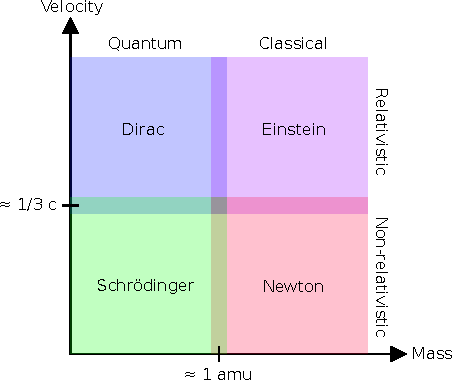
\includegraphics[scale=1.0]{Pics/dyneq}
\caption[Four regimes of dynamical equations]{Dynamical equations can be divided into four regimes, depending on the size and speed of the individual particles. Adapted form \cite{Jen2017}}
\label{fig:REGIMES}
\end{figure}

\section{The Electronic Schrödinger Equation}

\begin{quote}
  "Where did we get that [Schrödinger's equation] from? It's not possible to derive it from anything you know. It came out of the mind of Schrödinger."
  \begin{flushright}
    \small{--- \textit{Richard Feynman, The Feynman Lectures on Physics}}
  \end{flushright}
\end{quote}

If one is interested in describing the electron distribution in detail, the Schrödinger Equation (SEQ) is the best starting point. There is no formal, rigorous proof for the Schrödinger equation, similar to how Newton's second law cannot really be "derived", more than simply "motivated" by observation. 

As successful as the Schrödinger equation is, finding solutions to it is non-trivial. Different approximations may be applied to the SEQ to solve it more easily, without considerable loss of accuracy. 

\subsection{The Time-Independent Schrödinger Equation}

The potential energy operator is the only time-dependent part of the Hamiltonian:
\begin{equation}
\hat{H}(\mbf{r},t) = \hat{T}(\mbf{r}) + \hat{V}(\mbf{r},t)
\end{equation} 
\noindent For systems where the potential is time-independent, e.g. bound systems without external (electromagnetic) perturbation, the Hamiltonian is time-independent as well, which in turn allows to separate space and time variables. It can then be shown that the \emph{time-independent} Schrödinger equation takes the form
\begin{equation}
\hat{H}\Psi(\mbf{r}) = E \Psi(\mbf{r})
\end{equation}
\noindent where $E$ is the total energy of the system, and the eigenvalue of the wave function $\Psi$. The time-dependence is then simply reduced to a phase factor:
\begin{equation}
\Psi(\mbf{r},t) = e^{-iEt} \Psi(\mbf{r})
\end{equation}
\noindent 

\subsection{The Born-Oppenheimer Approximation}

Atomic nuclei are much heavier than electrons ($m_{proton} \approx 1836 m_{electron}$), and move much slower. To a good approximation, the nuclei can be assumed to be stationary from the point of view of electrons. This is known as the \emph{Born-Oppenheimer approximation}. The total Hamiltonian operator can be written in terms of the kinetic and potential operator of the nuclei ($n$) and electrons ($e$) as
\begin{equation}
\hat{H}_{tot} = \hat{T}_n + \hat{T}_e + \hat{V}_{ne} + \hat{V}_{ee} + \hat{V}_{nn}
\label{eq:FULLHAMILTONIAN}
\end{equation}
\noindent In the Born-Oppenheimer approximation, the kinetic energy of the nuclei $T_{nn}$ is neglected, and the nucleus-nucleus potential $V_{nn}$ is taken as a constant, which corresponds to neglecting the coupling between electrons and nuclei. This allows a separation of the electronic and nuclear variables. The remaining terms of Equation \ref{eq:FULLHAMILTONIAN} form the electronic Hamiltonian $\hat{H}_{elec}$. The solutions to the \emph{electronic Schrödinger equation}
\begin{equation}
\hat{H}_{elec} \Psi_{elec}(\mbf{r}_i, \mbf{R}_n ) = E_{elec}(\mbf{R}_n) \Psi_{elec}(\mbf{r}_i, \mbf{R}_n )
\end{equation}
\noindent produce the electronic wave function which depends on the (fixed) \emph{position} $\mbf{R}_n$ of the nuclei and no longer on the \emph{momentum} of the nuclei. The total energy
\begin{equation}
E_{tot}(\mbf{R}_n) = E_{elec}(\mbf{R}_n) + E_{nucl}(\mbf{R}_n)
\end{equation} 
\noindent provides a \emph{potential energy surface} (PES) on which the nuclei move. The PES can then be used to solve the nuclear Schrödinger equation to obtain information on vibrational, rotational and translational properties in the molecular system.

From this point onward, the subscript $elec$ is dropped, and only the electronic Schrödinger Equation is considered.

\section{Solutions to the Electronic Schrödinger Equation}

\subsection{Slater Determinants}

It is beneficial to first consider the wave function of a single electron. In single-atom systems, these functions take the form of "atomic orbitals" (AOs). Correspondingly, "molecular orbitals" (MOs) are defined as the single electron wave functions in a molecular system. These spatial orbital functions form the basis of the full electronic wave function.  

The Hamiltonian in \ref{eq:FULLHAMILTONIAN} only depends on the spatial coordinates. However, to fully describe an electron, spin also needs to be considered. This is done by introducing two orthonormal spin functions $\alpha(\omega)$ and $\beta(\omega)$ corresponding to spin-up ($\uparrow$) and spin-down ($\downarrow$), with the spin-coordinate $\omega$. For one spatial molecular orbital, this gives two possible \emph{spin-orbitals}
\begin{equation}
\phi(\mathbf{x}) = \left\lbrace\begin{matrix}
\varphi(\mathbf{r}) \alpha(\omega) \\
\varphi(\mathbf{r}) \beta(\omega)
\end{matrix} \right.
\end{equation}
\noindent where $\varphi$ are the \emph{spatial orbitals}, and $\mathbf{x}$ are the combined spatial and spin coordinates. The spin orbitals therefore depend on four variables.

To a first approximation, one may consider a molecular system to consist of $N$ \emph{non-interacting}, independent electrons. The Hamiltonian is then written as a sum of one-particle Hamiltonians 
\begin{equation}
\mathbf{H} = \sum_i^N \mathbf{h}_i 
\end{equation}
\noindent Electron correlation may be included in some average way by using \emph{effective} one-electron Hamiltonians, which is the basic working idea of the \emph{Hartree} method. The solution to the SEQ can then be expressed as a product of the one electron wave functions
\begin{equation}
\Psi^{HP}(\mbf{x}_1,\mbf{x}_2,...,\mbf{x}_N) = \phi(\mbf{x}_1) \phi(\mbf{x}_2) ... \phi(\mbf{x}_N)
\end{equation}
\noindent which is also known as \emph{Hartree product}. 

However, the Hartree product does not take into account the \emph{indistinguishability} of electrons. In what is known as the antisymmetry principle, a generalization of the Pauli exclusion principle, the wave function needs to fulfill 
\begin{equation}
\Psi(\mbf{x}_1,\mbf{x}_2) = - \Psi(\mbf{x}_2,\mbf{x}_1) 
\end{equation}
\noindent upon exchange of any two electrons in the system. This is most easily achieved by using \emph{Slater determinants} (SD). For a molecular system consisting of $N$ electrons distributed over $N$ spin orbitals $\phi_i$, the SD takes the form
\begin{equation}
\Psi_{SD}(\mbfx_1, \mbfx_2, \ldots, \mbfx_N) = \frac{1}{\sqrt{N!}}
\begin{vmatrix}
\phi_I(\mbfx_1) & \phi_J(\mbfx_1) & \ldots & \phi_P(\mbfx_1) \\
\phi_I(\mbfx_2) & \phi_J(\mbfx_2) & \ldots & \phi_P(\mbfx_2) \\
\vdots & \vdots & \ddots & \vdots \\
\phi_I(\mbfx_N) & \phi_J(\mbfx_N) & \ldots & \phi_P(\mbfx_N) \\
\end{vmatrix}
\end{equation}
\noindent Or, using the diagonal of the SD as a short-hand notation
\begin{equation}
\Psi_{SD}(\mbfx_1, \mbfx_2, \ldots, \mbfx_N) = \ket{\phi_I(\mbfx_1) , \phi_J(\mbfx_2), \ldots, \phi_P(\mbfx_N)}
\end{equation}

\subsection{The Fock Space}

A more generalized representation of the space of the antisymmetrized electron wave functions can be achieved by introducing the concept of occupation number (ON) vectors in the context of \emph{second quantization} (Appendix \ref{app:SECQUA}). In a system with $M$ possible states (which in the case of molecules correspond to spin molecular orbitals), the ON vectors take the form
\begin{equation}
\ket{\mbf{k}} = \ket{k_1, k_2, \ldots, k_M} = 
\left\lbrace
\begin{matrix}
1 \quad \textit{if $\phi_P$ occupied} \\
0   \quad \textit{if $\phi_P$ occupied}
\end{matrix}
\right.
\label{eq:ONVECTORS}
\end{equation}
\noindent The occupation number is 1 if $\phi_P$ is present in the SD, and 0 if not. Together, all possible ON vectors in Equation \ref{eq:ONVECTORS} form an orthonormal abstract vector space, known as Fock space. The Fock space formed by $N$ electrons distributed over $M$ orbitals is denoted as $F(M,N)$ with total dimension equal to the binomial coefficient $\smash{\binom{M}{N}}$. The sum of the occupation numbers in the ON vectors gives the total number of electrons
\begin{equation}
N = \sum_i^M k_i
\end{equation}
\noindent The special Fock space $F(0,M)$ contains a single vector known as the vacuum state with
\begin{align}
&\ket{vac} = \ket{0_1, 0_2, \ldots, 0_M} \\
&\bra{vac}\ket{vac} = 1
\end{align}
\noindent The ON vectors in $F(M,N)$ can alternatively be expressed in terms of the vacuum state from $F(M,0)$ using creation operators
\begin{equation}
\ket{\mbf{k}} = \left[ \prod_{P=1}^M (a\pdg_P)^{k_P} \right] \ket{vac}
\end{equation}
\noindent In second quantization, the antisymmetry principle of the wave function is guaranteed by the anticommutator relationship of the annihilation and creation operators $a_P$ and $a\pdg_P$ which act on the ON vectors.

\subsection{Exact Solution and Standard Models}

The simplest approach to solving the electronic SEQ is by approximating the exact wave function $\ket{\Psi}$ using a single Slater determinant where the electrons occupy the lowest lying molecular orbitals. The Hartree-Fock method is an example of a \emph{single-determinant method} and finds \emph{the} single best Slater determinant for $\ket{\Psi}$. In Fock space, the best possible determinant is represented by the ON vector where the $N$ lowest lying orbitals are occupied. 

As will be discussed in more detail later, a single-determinant treatment of the electronic wave function is insufficient to fully capture \emph{electron correlation}. The electron correlation energy is formerly defined as the difference between the Hartree-Fock energy and the \emph{exact} energy of $\ket{\Psi}$
\begin{equation}
E_{correlation} = E_{HF} - E_{exact}
\end{equation}
\noindent although the Hartree-Fock wave function does include correlation effects to some degree. In a more general sense, electron correlation is a broad term for any interactions between electrons that make their movement depend on each other, or \emph{correlate} with each other (see Section \ref{sec:CORRELATION}). 

In order to improve on the HF approximation, it is important to add additional Slater determinants. These SDs can be generated from the HF reference wave function by replacing the occupied MOs $\phi_I$ in a reference Slater determinant by one or multiple orbitals $\phi_A$ which were previously unoccupied. This effectively corresponds to exciting one or more electrons from their occupied molecular orbitals $I,J,..$ to unoccupied, or $virtual$ orbitals $A,B,..$. These excited Slater determinants can be classified by the number of electrons they excite and are often referred to as singles, doubles, triples and so on.
\begin{alignat}{2}
\ket{\Phi_0} &= \ket{\HFWFN} \quad & \text{Reference} \\
\ket{\Phi_{I}^{A}} &= a\pdg_A a_I \ket{\HFWFN} \quad & \text{Singles}  \\
\ket{\Phi_{IJ}^{AB}} &= a\pdg_A a_I a\pdg_B a_J \ket{\HFWFN} \quad & \text{Doubles} \\
\ket{\Phi_{IJK}^{ABC}} &= a\pdg_A a_I a\pdg_B a_J a\pdg_C a_K \ket{\HFWFN} \quad & \text{Triples} 
\end{alignat}
\noindent Alternatively, singles states are known as 1-particle-1-hole (1p-1h or simply p-h) states, doubles as 2-particle-2-hole (2p-2h) and so on, due to the excitation operators effectively creating \emph{holes} in the reference determinant and adding \emph{particles} in higher lying orbitals instead. 

The exact solution to the electronic Schrödinger equation is then given by the sum of the Hartree-Fock wave function and all possible ON vectors in $F(M,N)$
\begin{equation}
\ket{\Psi} = c_0 \ket{\HFWFN} + \sum^{\binom{M}{N}-1}_{i=1} c_i  \ket{i} 
\label{eq:EXACTWF}
\end{equation}  
\noindent Equation \ref{eq:EXACTWF} offers a systematic approach to improve on the Hartree Fock method, by increasing (1) the number of Slater determinants and (2) the basis set size $M$, and gives rise to a hierarchy of methods (Figure \ref{fig:STANDARDMODEL}). Correlated electronic structure methods mainly differ by how they determine the expansion coefficients $c$. For all but the smallest systems, the full $F(M,N)$ Fock space cannot be used in calculations due to the total number of ON vectors which increases binomially with $\smash{\binom{M}{N}}$, and hence the number of coefficients to be determined. In practice, the Fock space is \emph{truncated} to some degree.

\begin{figure}
\centering
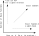
\includegraphics[scale=2.0]{Pics/standardmodel}
\caption[Converging towards the exact wave function]{The wave function converges to the exact solution in the limit of an infinitely large basis set that spans the molecular orbitals, and an infinitely large correlation space spanned by the Slater Determinants.}
\label{fig:STANDARDMODEL}
\end{figure}

\emph{Multi-determinant} methods like configuration interaction (CI) or coupled cluster (CC) use the Hartree Fock wave function as reference from which they generate singles, doubles, triples ... SDs. By truncating at different excitation levels, one gets a hierarchy of CI/CC methods which recover different amounts of correlation energy (e.g. CIS, CISD, CISDT ...). Multi-determinant methods are mainly suited to recover dynamic correlation.

For systems with strong static correlation, additionally, a multi-reference approach is needed. Here, the excited SDs are generated from multiple reference states rather than only from HF. Methods include multi-reference CI (MRCI) and multi-reference CC (MRCC). The reference states are traditionally obtained from multi-configurational self-consistent-field methods (MCSCF) like the complete active space SCF (CASSCF) or restricted active space SCF (RASSCF). MCSCF is a combination of HF and CI, which both optimizes the HF molecular coefficients and the CI expansion coefficients. Multi-reference methods methods mainly recover \emph{static correlation}. 

\subsection{The Variational Method}

The time-independent Schrödinger equation takes the form of an eigenvalue problem
\begin{equation}
\hat{H} \ket{\Psi_i} = E_i \ket{\Psi_i} \qquad i=0,1,2,...\infty
\label{eq:SEQINFTY}
\end{equation}
\noindent where the infinite set of exact solutions $\ket{\Psi_i}$ with eigenvalues $E_i$ forms an orthonormal basis
\begin{equation}
\bra{\Psi_i}\ket{\Psi_j} = \delta_{ij}
\end{equation} 
\noindent A trial wave function can be expanded in the basis of exact solutions with coefficients $c$ as
\begin{equation}
\ket{\tPsi} = \sum_i c_i \ket{\Psi_i}
\label{eq:trialwave}
\end{equation}
\noindent The \emph{variation principle} states that the expectation value of the Hamiltonian of an approximate wave function of the form \ref{eq:trialwave} is an upper bound to the exact ground state energy. This statement can be expressed as
\begin{equation}
\frac{\bra{\tPsi}\hat{H}\ket{\tPsi}}{\vphantom{\widetilde{\Psi}} \bra{\tPsi}\ket{\tPsi}} \geq E_0
\end{equation}
\noindent The equality only holds when $\ket{\tPsi}$ is equal to the exact solution $\ket{\Psi_0}$. One can recast the eigenvalue problem \ref{eq:SEQINFTY} as a variational optimization problem where the energy is a functional of a trial wave function
\begin{equation}
E[\tPsi] = \frac{\bra{\tPsi}\hat{H}\ket{\tPsi}}{\vphantom{\widetilde{\Psi}} \bra{\tPsi}\ket{\tPsi}}
\end{equation}
\noindent The saddle points of the energy functional then correspond to the exact solutions of the Schrödinger equation. The variational approach to the SEQ provides a powerful tool to solve a wide variety of problems in electronic structure theory.

The trial wave function depends on a set of coefficients $c$, and hence the energy functional will also depend on these coefficients. In general, determining the coefficients which minimize the functional is very difficult. However, a more simple approach of the variational method can be obtained by using a linear ansatz where the trial function is expanded in a fixed N-dimensional set of orthonormal basis functions $\ket{\phi}$
\begin{equation}
\ket{\tPsi} = \sum^N_i c_i \ket{\phi_i}
\end{equation}
By using Lagrange's method of undetermined multipliers
\begin{align}
\mathcal{L}(\mbf{c},E) &= \bra{\tPsi}\hat{H}\ket{\tPsi} - E(\bra{\tPsi}\ket{\tPsi} - 1) \\
\frac{\partial \mathcal{L}}{\partial \mathcal{\mbf{c}}} &= 0
\end{align}
\noindent it is possible to show that the variational problem corresponds to solving the eigenvalue problem involving the Hamiltonian matrix $\mbf{H}$:
\begin{equation}
\mbf{H}\mbf{c}_n = E_n \mbf{c_n}
\end{equation}
\noindent Or, in a more general form
\begin{equation}
\mbf{H}\mbf{C} = \mbf{C}\mbf{E}
\end{equation}
\noindent Here, $\mbf{C}$ is a $N$ by $N$ coefficient matrix containing $N$ column coefficient vectors $\mbf{c}_n$ ($n$ = $0...N$) which describe $N$ possible solutions for the trial wave function $\ket{\tPsi}$. $\mbf{E}$ is a diagonal matrix containing the eigenvalues $E_n$. This approach of finding approximate solutions to the eigenvalue problem \ref{eq:SEQINFTY} is known as the \emph{linear variational method}. 

\section{Hartree-Fock}

The Hartree-Fock method is central to electronic structure theory. It is computationally inexpensive, and is still routinely used in qualitative studies of large molecules, even if it does not accurately account for electron correlation. It also serves as the starting point for correlated methods. Only a few computational methods actually bypass the solution to the Hartree-Fock equations, firmly cementing its place in quantum chemistry.

\subsection{The Hartree Fock Equations}

Recall the structure of the electronic Hamiltonian
\begin{equation}
\hat{H} = \hat{T}_e + \hat{V}_{ne} + \hat{V}_{ee} + \hat{V}_{nn}
\end{equation}
\noindent with
\begin{alignat}{2}
\hat{T}_e &= -\sum_i^N \frac{1}{2} \nabla_i^2 & \qquad \textrm{kinetic energy of electrons} \\
\hat{V}_{ne} &= -\sum_a^{N_{nuc}} \sum_i^N \frac{Z_a}{\mid\mbf{R}_a - \mbf{r}_i\mid} & \qquad \textrm{nuclei-electron repulsion} \\
\hat{V}_{ee} &= \frac{1}{2} \sum^N_i \sum^N_{j \neq i} \frac{1}{\mid \mbf{r}_i - \mbf{r}_j\mid} & \qquad \textrm{electron-electron repulsion} \\
\hat{V}_{nn} &= \frac{1}{2}\sum_a^{N_{nuc}} \sum_{b \neq a}^{N_{nuc}} \frac{Z_a Z_b}{\mid \mbf{R}_a - \mbf{R}_b \mid} & \qquad \textrm{nuclei-nuclei repulsion} 
\end{alignat}
\noindent In Hartree-Fock theory, the electrons are treated as independent particles. One can therefore ignore the coupling between electrons in $\hat{V}_{ee}$ and express the Hamiltonian as a sum of an effective one-electron operator $\mbf{f}$, also known as the \emph{Fock} operator, of the form
\begin{align}
\hat{H} &= \sum_i \hat{f}_i =  \sum_i \hat{h}_i + \frac{1}{2} \sum_i \sum_{j \neq i} \hat{g}_{ij} \\
\hat{h}_i &= -\frac{1}{2}\nabla_i^2 - \sum_a^{N_{nuc}} \frac{Z_a}{\mid \mbf{R}_a - \mbf{r}_i |} \\
\hat{g}_{ij} &= \frac{1}{\mid \mbf{r}_i - \mbf{r}_j \mid}
\end{align}
\noindent The one-electron operator $\hat{h}$, also known as the \emph{core} Hamiltonian describes the movement of the electrons in the field of the nuclei. The two-electron operator $\mbf{g}_{ij}$ gives the average potential (or "field") experienced by electron $i$ due to the presence of all the other electrons $j$. For this reason, Hartree-Fock is also known the \emph{mean-field} approximation. In second quantization, the Fock operator takes the form
\begin{equation}
\hat{f} = \sum^{M}_{PQ} h_{PQ} a\pdg_P a_Q + \frac{1}{2} \sum^{M}_{PQRS} g_{PQRS} a\pdg_P a\pdg_R a_S a_Q
\label{eq:FOCK2Q}
\end{equation}
\noindent with the matrix elements of the one and two electron operators given by
\begin{align}
h_{PQ} &= \bra{\phi_P} \mbf{h} \ket{\phi_Q} = \int \phi_P^*(\mbf{x}) h(\mbf{x}) \phi_Q(\mbf{x}) d\mbf{x} \\
g_{PQRS} &= \bra{PQ}\ket{RS} = \int\int \phi_P^*(\mbf{x}_1) \phi^*_R(\mbf{x}_2) g(\mbf{x}_1,\mbf{x}_2) \phi_Q(\mbf{x}_1) \phi_S(\mbf{x}_2) d\mbf{x}_1 d\mbf{x}_2
\end{align} 
\noindent The elements $g_{PQRS}$ are known as the two-electron repulsion integrals. Calculating the expectation values for the Fock operator in \ref{eq:FOCK2Q} using second quantization gives the matrix elements \cite{Hel2000}
\begin{equation}
\begin{split}
f_{PQ} &= \bra{\phi_P} \mbf{f} \ket{\phi_Q} \\
	&= h_{PQ} + \sum_{I}^N \frac{1}{2} (g_{PQII} - g_{PIIQ}) \\
	&= h_{PQ} + \frac{1}{2} (J_{PQ} - K_{PQ})
\end{split}
\end{equation} 
\noindent The symmetric matrix with entries $f_{PQ}$ is also known as the \emph{Fock matrix}. $\mbf{J}$ is the \emph{coulomb matrix} and describes electron correlation due to the coulomb potential (coulomb correlation), and $\mbf{K}$ is the exchange matrix describing the electron correlation which arises due to the Pauli exclusion principle (Fermi correlation). The exchange contributions have no classical counterpart and arise purely from quantum mechanical considerations. 

In the special basis where the Fock matrix is diagonal
\begin{equation}
f_{PQ} = \delta_{PQ} \eps_P 
\end{equation}
\noindent the one-electron eigenfunctions of the Fock operator 
\begin{equation}
\mbf{f} \ket{\phi_P} = \eps_P \ket{\phi_P} 
\label{eq:HFEQ}
\end{equation} 
\noindent are known as the \emph{canonical molecular spin orbitals}, and the eigenvalues are the \emph{molecular orbital energies}. Solving the \emph{canonical Hartree-Fock equation} \ref{eq:HFEQ} gives the MOs which form the basis of the Hartree-Fock wave function. It should be stressed that the total electronic Hartree-Fock energy is not the sum of the individual MO energies, but is given by the expectation value of the Hamiltonian 
\begin{equation}
E_{HF} = \bra{\HFWFN}\hat{H}\ket{\HFWFN} = \sum_{I}^{N} h_{II} + \frac{1}{2} \sum_{I}^{N} \left( J_{II} - K_{II} \right) 
\end{equation}
\noindent which is equivalent to the \emph{trace} of the Hamiltonian matrix $\mbf{H}$. The index $I$ runs over all occupied spin molecular orbitals. For $N$ electrons distributed over $M$ MOs, there are $N$ occupied orbitals with $\eps_I < 0$ and $M-N$ virtual orbitals with $\eps_A > 0$. 

\subsection{The Basis Set Approximation}

Up until this point, the electronic wave function was constructed from Slater determinants of molecular spin orbitals. Virtually all applications use a basis set expansion to express the unknown MOs in terms of known functions, conventionally called \emph{atomic orbitals}. Any type of function can be used, e.g. exponentials, Gaussians, polynomials or plane waves. The molecular orbitals are then expressed as a \emph{linear combination of atomic orbitals} (LCAO)
\begin{equation}
\ket{\phi_i} = \sum_i^{M_{basis}} c_{i\mu} \chi_{\mu} 
\end{equation}
\noindent For molecular systems, there are two types of basis functions that are generally used, namely Slater Type Orbitals (STO) and Gaussian Type Orbitals (GTO):

\begin{align}
\chi_{\zeta, n, l, m}^{STO} (r,\theta ,\phi ) &= N Y_{l,m} (\theta , \phi ) r^{n-1} e^{-\zeta r}
\\
\chi_{\zeta, n, l, m}^{GTO} (r,\theta ,\phi ) &= N Y_{l,m} (\theta , \phi ) r^{2n - 2 - l} e^{-\zeta r^2}
\end{align}

\noindent where N is a normalization constant, $Y_{l,m}$ are spherical harmonics, and $\{n,l,m\}$ are the principal, angular momentum and magnetic quantum number respectively. There are two major differences between STOs and GTOs. At r = 0, STOs have finite slope and GTOs have zero slope. For large r values, GTOs decay much more rapidly than STOs. From an electronic structure point of view, one would prefer to use STOs, as they describe the qualitative features of molecular orbitals better than GTOs. Roughly three time as many GTOs are necessary to obtain the same accuracy as with STOs. Nonetheless, GTOs are preferred, as their drawbacks are outweighed by the relative ease with which their integrals can be evaluated compared to STOs.

\subsection{Working Equations for Restricted and Unrestricted Hartree\-/Fock}

For reasons of efficient implementation, it is useful to separate out different electron spin components. The Fock matrix has four spin blocks: $F_{\alpha\alpha}$, $F_{\alpha\beta}$, $F_{\beta\alpha}$ and $F_{\beta\beta}$. The Fock matrix in the canonical basis is diagonal, and therefore only the diagonal blocks  $F_{\alpha\alpha}$ and $F_{\beta\beta}$ are important. Introducing the notation $\olI$ for MOs with spin $\sigma'$, and $I$ with opposite spin $\sigma$, the matrix elements of a spin block are given by
\begin{equation}
\begin{split}
f_{PQ}^{\sigma} &= h_{PQ}^{\sigma} + \frac{1}{2} \left\lbrace \sum^{N_{\sigma}}_{PQ}\sum^{N_{\sigma}}_{I} \cn{PQ}{II} - \cn{PI}{QI}  - \sum^{N_{\sigma}}_{PQ}\sum^{N_{\sigma'}}_{I} \cn{PQ}{\olJ\olJ} - \cn{P\olJ}{Q\olJ} \right\rbrace \\
&= h_{PQ}^{\sigma} + \sum^{N_{\sigma}}_{PQ} J^{\sigma}_{PQ} - K^{\sigma}_{PQ} + J^{\sigma'}_{PQ} - K^{\sigma'}_{PQ}
\end{split}
\end{equation}
\noindent The opposite spin block $f_{PQ}^{\sigma'}$ is obtained by substituting indices with a bar by indices without a bar and vice-versa. Spin separation yields two coupled sets of equations for alpha and beta MOs
\begin{equation}
\begin{split}
\mbf{f}^{\alpha} \sket{\phi^{\alpha}_I} &= \eps^{\alpha}_I \sket{\phi^{\alpha}_I} \\
\mbf{f}^{\beta} \sket{\phi^{\beta}_I} &= \eps^{\beta}_I \sket{\phi^{\beta}_I} 
\end{split}
\label{eq:UHF}
\end{equation} 
\noindent These are known as the unrestricted Hartree-Fock equations (UHF). For closed-shell molecules with equal number of alpha and beta electrons, the spatial part of the MOs is the same for both spins. The expression for the Fock matrix then further simplifies to 
\begin{equation}
f_{ij} = h_{ij} + 2J_{ij} - K_{ij} 
\end{equation}
\begin{equation}
\mbf{f} \ket{\phi_i} = \eps_i \ket{\phi_i}
\label{eq:RHF}
\end{equation}
\noindent The equations in \ref{eq:RHF} are known as the restricted Hartree-Fock (RHF) equations. 

\noindent Using the linear variatonal method explained in the previous section for the MO trial functions expressed as a linear combination of $N_{bas}$ AO basis functions, the eigenvalue problem for RHF can be recast in matrix form as
\begin{align}
\mbf{F} \mbf{C} &= \mbf{C} \mbf{E} 
\end{align}
\noindent with the MO coefficient matrix $\mbf{C}$ and the Fock matrix $\mbf{F}$ in the AO basis given by
\begin{align}
F_{\mu\nu} &= H^{core}_{\mu\nu} + \sum_{\lambda\sigma}^{N_{basis}} \left[ 2 \cn{\mu\nu}{\sigma\lambda} P_{\lambda\sigma} - \cn{\mu\sigma}{\nu\lambda} P_{\lambda\sigma} \right] \\
&= H^{core}_{\mu\nu} + 2 J_{\mu\nu} - K_{\mu\nu} 
\end{align}
\noindent The symmetric matrix $\mbf{P}$ is the so-called atomic orbital density matrix (DM) of the form
\begin{equation}
P_{\mu\nu} = \sum_i^{N_{occ}} C_{\mu i} C_{\nu i} 
\end{equation}
\noindent A similar expressions is found for UHF
\begin{equation}
\begin{split}
F_{\mu\nu}^{\sigma} &= H^{core}_{\mu\nu} + \sum_{\lambda\sigma}^{N_{basis}} \left( \cn{\mu\nu}{\sigma\lambda} P^{T}_{\lambda\sigma} - \cn{\mu\sigma}{\nu\lambda} P^{\sigma}_{\lambda\sigma} \right) \\
P^T_{\mu\nu} &= P^{\sigma}_{\mu\nu} + P^{\sigma'}_{\mu\nu} 
\end{split}
\end{equation}
\noindent where the AO spin-density matrices $\mbf{P}^{\sigma}$ are defined as the product of the corresponding coefficient matrices with spin $\sigma$.  

\subsection{The Self-Consistent Field Method}

In general, the atomic orbitals are not orthogonal. The overlap matrix $\mbf{S}$ is defined as 
\begin{equation}
S_{\mu\nu} = \int \chi_{\mu}^*(\mbf{r}) \chi_{\nu}^*(\mbf{r}) d\mbf{r}
\end{equation}
\noindent with diagonal entries $S_{\mu\mu} = 1$, and off-diagonal elements $0 < \left\lvert S_{\mu\nu} \right\rvert < 1$. The eigenvalue problem for RHF then takes the more general form
\begin{equation}
\mbf{F} \mbf{C} = \mbf{SC} \mbf{E}
\label{eq:RHALL}
\end{equation}
\noindent The equations in \ref{eq:RHALL} are known as the \emph{Roothan-Hall equations} (RH). In the unrestricted case, they are called the \emph{Pople-Nesbet equations} (PN) which are given by
\begin{align}
\mbf{F}^{\alpha} \mbf{C}^{\alpha} &= \mbf{SC}^{\alpha} \mbf{E}^{\alpha} \\
\mbf{F}^{\beta} \mbf{C}^{\beta} &= \mbf{SC}^{\beta} \mbf{E}^{\beta}
\end{align}  
\noindent The Fock matrix is constructed using the coefficient matrices $\mbf{C}$ to compute the density matrix $\mbf{P}$. This means that the RH (and PN) equations depend on their own solution and must be solved iteratively. Popular choices for iterative schemes include \emph{Newton's} method and the \emph{self-consistent field} (SCF) method, with the latter being the most straight-forward one to implement. 

The SCF procedure is summarized in Algorithm \ref{algo:SCF}. At every iteration, the Fock matrix is diagonalized to obtain a new guess for the density matrix, which is used for constructing the Fock matrix in the next step. These steps are repeated until \emph{self-consistency} is reached. There are different ways to test for convergence, the simplest being the Hartree-Fock energy difference between subsequent iterations. A more rigorous bound is given by the matrix norm of the error vector $\mbf{e}$
\begin{equation}
\mbf{e} = \mbf{FPS} - \mbf{SPF} 
\end{equation}
\noindent At convergence, the density matrix has to commute with the Fock matrix through the overlap matrix. 

\begin{algorithm}
\KwIn{Molecule with nuclear coordinates $\{\mbf{R}_A\}$, atomic numbers $\{Z_A\}$, number of electrons $N$ and basis set $\{\chi_{\mu}\}$}
\KwOut{The matrices $\mbf{F}$, $\mbf{P}$, $\mbf{C}$ and $\mbf{E}$} 
Calculate all one- and two electron integrals
\\
Compute the transformation matrix $\mbf{X}$ from the overlap matrix $\mbf{S}$ with
\begin{equation}
\mbf{X}\pdg \mbf{SX} = \mbf{1} 
\end{equation}
\\
Generate a set of guess orbitals to compute an initial guess density $\mbf{P}$
\\
\While{not converged}{
	Construct the Fock matrix $\mbf{F}$ using the current guess density
	\\
	Orthogonalize the Fock matrix $\mbf{F'} = \mbf{X}\pdg \mbf{FX}$
	\\
	Diagonalize $\mbf{F}'$ to obtain the new orthogonalized MO coefficient matrices $\mbf{C}'$
	\\
	Compute $\mbf{C} = \mbf{X}\mbf{C}$
	\\
	Form the new density $\mbf{P} = \mbf{CC}^T$
	\\
	Check convergence using certain criteria
}
\caption{Hartree-Fock Self-Consistent Field}
\label{algo:SCF}
\end{algorithm}

\subsubsection{SCF Initial Guesses}

The preiteration steps compute the two-electron integrals, the transformation matrix $\mbf{X}$ and a set of guess orbitals. There are different methods for generating a guess. The closer the guess is to the solution, the fewer SCF iterations are needed which saves time. The simplest method consists of using a null matrix for $\mbf{P}$, which corresponds to setting the Fock matrix to the core Hamiltonian $\mbf{H}^{core}$. Diagonalization then gives the guess orbitals. The core Hamiltonian gives a sufficiently close starting guess for small molecules, but is unsuitable for larger molecules. 

The most popular and efficient method at the time of writing is the superposition of atomic densities (SAD) \cite{Van2006}. For each type of atom in the molecule, an atomic HF calculation is carried out which gives the atomic density matrix for this atom type. The molecular guess density matrix is then constructed by setting its diagonal blocks to the atomic densities. The SAD method generates densities that are quite close to the solution. For implementation details, see Appendix \ref{sec:SCFGUESS}.

An alternative starting guess can be obtained by first carrying out a HF calculation with a smaller basis set using the core or SAD guess, and then projecting the density matrix onto the larger basis set (Appendix \ref{sec:SCFGUESS}). This method is especially useful for larger basis sets.  

\subsubsection{SCF convergence}

There is no guarantee that the SCF procedure converges. For small molecules and equilibrium geometries, the unmodified SCF procedure converges quite smoothly. For large, diffuse basis sets or distorted geometries, additional modifications to the algorithms might be necessary:
\begin{enumerate}
\item Direct inversion of the iterative subspace (DIIS): the previous Fock matrices are used for extrapolation to generate a better Fock matrix (section \ref{sec:DIIS})
\item Damping: A damping factor $\omega$ is introduced and the density matrix is replaced by a weighted average $\mbf{P}'_{n+1} = \omega \mbf{D}_n + (1-\omega)\mbf{D}_{n+1}$. Damping is especially useful when the SCF energy oscillates around the equilibrium
\item Level shifting: It has been shown that raising the energy of the virtual orbitals guarantees convergence, at the cost of a decreased convergence rate
\end{enumerate} 

\subsection{Brillouin's Theorem and Orbital Rotations}

The Fock matrix can be divided into four distinct blocks: occupied-occupied, occupied-virtual, virtual-occupied and virtual-virtual. The terms "particle" (p) and "hole" (h) may be used instead of occupied and virtual. In the special case where the orbitals are the canonical MOs, the Fock matrix is diagonal. This is known as the \emph{canonical condition} for the HF wave function. However, diagonality is not necessary for obtaining a valid HF wave function. The general Hartree-Fock equations take the form
\begin{equation}
\hat{f} \phi_P = \sum_{PR} \lambda_{PR} \phi_R
\end{equation}
\noindent Where $\lambda$ are the Lagrange multipliers. For non-canonical MOs, the p-p and h-h are non-diagonal, with elements $\lambda_{IJ}$ and $\lambda_{AB}$ respectively. The off-diagonal elements are computed as
\begin{equation}
f_{IA} = \sbra{\HFWFN}\hat{f}\sket{a\pdg_A a_I \HFWFN} = 0
\end{equation}
\noindent and are zero by virtue of \emph{Brillouin's theorem} for any valid HF wave function. This is also known as the \emph{variational condition}; it is an alternative formulation of the variational principle (see \cite{Hel2000}, section 10.3.5).

The Hartree-Fock energy is therefore stable under unitary rotations
\begin{equation}
\phi_{I'} = \mbf{U} \phi_I \qquad U\pdg U = \mbf{U}
\end{equation}
\noindent The canonical MOs may be rotated to another orbital MO basis with smaller spatial extent, also known as localized molecular orbitals (see Section \ref{sec:ABCLMO}).

\section{Electron Correlation \label{sec:CORRELATION}}

In the Hartree-Fock method, the electron-electron interaction is replaced by an average interaction. For large basis sets, HF is actually able to recover approximately 99\% of the total energy. Unfortunately, the remaining 1\%, the correlation energy, is often important to compute chemical properties with sufficient accuracy.

Electron correlation arises from electrons trying to avoid each other due to coulombic repulsion (coulomb correlation) and the antisymmetry principle (Fermi correlation). This in turn leads to a region of space around each electron where the probability of finding another electron is reduced, typically known as the \emph{coulomb hole} for electrons of opposite spin, and \emph{Fermi hole} for electrons of the same spin. 

Another distinction is often drawn between \emph{dynamic correlation} and \emph{static correlation}, although there exists no formal definition. Dynamic correlation generally describes the correlated movement of electrons due to their "instantaneous mutual repulsion" \cite{Jen2017}. For example, in the ground-state Helium atom, electron correlation is purely dynamical. Static (or non-dynamic) correlation on the other hand arises in the case of near\-/degeneracy, where multiple configurations of similar energy contribute to the ground-state wave function. To show the difference between these two two types of correlation, the dissociation of the H$_2$ molecule is often taken as an illustrative example. At equilibrium distance, correlation is mostly dynamic, and the ground-state can be well described as a singlet state. In the dissociation limit, electrons may be coupled to yield either a singlet \emph{or} a triplet, as the energy difference between those two states vanishes. The correlation in the system is then entirely static. There is no clear-cut line between dynamic and static correlation, but it offers a useful classification for correlation effects.

To fully capture both dynamic and static correlation, it is crucial to add additional Slater determinants as mentioned previously. Methods which generate excited Slater determinants from a single reference SD recover mostly dynamical correlation: electrons are disturbed through their instantaneous repulsion and are excited to higher spin orbitals, hence the need of additional excited-type SDs. Methods generating SDs from multiple references recover mostly static correlation. At the theoretical limit (i.e. the full configuration space), both approaches eventually recover all correlation effects. It is therefore the responsibility of the computational chemist to choose the correct method that best fits the problem at hand.

Any electronic structure method that improves on the HF wave function is usually referred to as a "correlated method". Hartree-Fock, by convention, is an "uncorrelated method". 

For the rest of this report, only single-reference methods are considered.

\section{Configuration Interaction}

\subsection{The CI Matrix}

Configuration interaction (CI) is the simplest and one of the oldest examples of a correlated electronic structure method. The CI wave function takes the general form
\begin{equation}
\ket{\CIWFN} = \sket{\Psi_0} + \sum_{IA} c_{I}^{A} \sket{\Phi_{IA}} + \sum_{\substack{I < J \\ A < B}} c_{IJ}^{AB} \sket{\Phi_{IJ}^{AB}} + \sum_{\substack{I < J < K \\ A < B < C}} c_{IJK}^{ABC} \sket{\Phi_{IJK}^{ABC}} + \dots
\end{equation}
\noindent summing all SDs of all possible types (singles, doubles, triples...). $\Phi_0$ is the reference wave function, here taken as the HF ground state. Whereas the HF wave function was a linear combination of molecular orbitals, the CI wave function is a linear expansion of SDs. Similarly, the CI expansion coefficient matrix $\mbf{C}$ is determined variationally
\begin{equation}
\frac{\partial}{\partial C_i} \frac{\sbra{\CIWFN}\hat{H}\sket{\CIWFN}}{\sbraket{\CIWFN}{\CIWFN}} = 0
\end{equation}
\noindent which, as was shown before, reduces to the eigenvalue problem
\begin{equation}
\mbf{H}\mbf{C} = \mbf{C}\mbf{E}
\end{equation}
\noindent The matrix $\mbf{H}$ is also known as the \emph{CI matrix}. Using the notation $\ket{S}$, $\ket{D}$, $\ket{T}$, ... to denote the set of singles, doubles, triples ... SDs, the CI matrix takes the form
\begin{equation}
\begin{bmatrix}
\bra{\Phi_0}\mbf{H}\ket{\Phi_0} & 0 & \bra{\Phi_0}\mbf{H}\ket{D} & 0 & 0 & \ldots \\
0 & \bra{S}\mbf{H}\ket{S} & \bra{S}\mbf{H}\ket{D} & \bra{S}\mbf{H}\ket{T} & 0 & \ldots \\
\bra{D}\mbf{H}\ket{\Phi_0} & \bra{D}\mbf{H}\ket{S} & \bra{D}\mbf{H}\ket{D} & \bra{D}\mbf{H}\ket{T} & \bra{D}\mbf{H}\ket{Q} & \ldots \\
0 & \bra{T}\mbf{H}\ket{S} & \bra{T}\mbf{H}\ket{D} & \bra{T}\mbf{H}\ket{T} & \bra{T}\mbf{H}\ket{Q} & \ldots \\
0 & 0 & \bra{D}\mbf{H}\ket{Q} & \bra{T}\mbf{H}\ket{Q} & \bra{Q}\mbf{H}\ket{Q} & \ldots \\
\vdots & \vdots & \vdots & \vdots & \vdots & \ddots  
\end{bmatrix}
\end{equation}
\noindent In analogy to the Fock matrix, some blocks in the CI matrix are zero. Brillouin's theorem states that there is no coupling between the ground state and the singlet states. That does not imply that they do not contribute to the CI energy at all. Singles mix \emph{indirectly} via doubles. Moreover, matrix blocks of the Hamiltonian between two SDs which differ by more than two spin orbitals are also zero. Triples mix with doubles and singles, but not with the ground state.

A more compact representation of the CI matrix is obtained by taking linear combinations of SDs in the same excitation manifold, known as configuration state functions (CSF) or spin-adapted configurations (SAC). The CSFs form a basis smaller than that composed of all individual SDs which leads to computational savings. However, CSFs were primarly introduced to preserve the spin symmetry of the ground state, or in other words, CSFs are eigenfunctions of the $\mbf{S}^2$ operator. If the HF ground state is a singlet, a non-spin-symmetric CI basis may lead to the CI wave function being a mixture of singlet and triplet determinants. 

\subsection{Truncated CI}

Full CI, i.e. including all excitation manifolds, is only computationally feasible for the smallest molecules, due to the binomial increase in the number of SDs as a function of system and basis set size. For this reason, the CI wave function is often truncated at a given excitation level. Including only singles gives configuration interaction with singles (CIS), including singles and doubles yields configuration interaction with singles and doubles (CISD), etc. Higher order methods recover a larger fraction of the correlation energy, but come at a higher computational cost.

It should be noted that the energy of the CIS wave function is equal to the HF energy due to Brillouin's theorem, and hence does not contribute to the correlation energy of the ground state.  

\subsection{Solving the CI Eigenvalue Problem}

Even at relatively low truncation levels, the number of matrix elements have a quite steep polynomial scaling with $\ccpx{6}$ for CISD and $\ccpx{8}$ for CISDT. In most cases however, only the few lowest eigenvalues are needed. Davidson's method of matrix diagonalization (section \ref{sec:DAV}) was specifically developed to tackle this problem. Rather than storing the whole matrix, only matrix-vector products need to be computed
\begin{equation}
\mbf{r} = \mbf{M}_{CI} \mbf{u}
\end{equation}
\noindent Closed expressions can be derived and the full matrix is not explicitly needed, but generated on-the-fly. 

\subsection{Size Consistency and Size Extensivity}

Over the years, single-reference truncated CI methods have fallen out of favor for more sophisticated methods, due to CI not being size-consistent and size-extensive. \emph{Size-consistency} refers to the idea that the energy of two non-interacting systems $A$ and $B$ should be equal to the sum of their individual energies obtained from two different calculations:
\begin{equation}
E(A+B) = E(A) + E(B)
\end{equation}
\noindent \emph{Size-extensivity} is a closely-related criterion that states that the energy should be a linear function of the number of electrons , i.e. the energies of small and large molecules have similar errors, which is important for comparing properties \cite{You2004}. As the system size increases, truncated CI recovers less and less of the total correlation energy.

\section{Coupled Cluster}

The coupled-cluster (CC) approximation offers a more sophisticated picture of electron correlation than CI, and has become one of the most successful and accurate \emph{ab initio} correlated methods. It is both size-consistent and size-extensive.

\subsection{Pair Clusters}

Consider a system composed of two electrons, occupying the orbitals $I$ and $J$ in the independent particle model. Correlation manifests itself by the electrons' instantaneous repulsion and excitation into higher lying orbitals. Mathematically, this may be expressed as \cite{Hel2000}
\begin{equation}
a\pdg_I a\pdg_J + \sum_{A > B} t_{IJ}^{AB} a\pdg_A a\pdg_B = \left( 1 + t_{IJ}^{AB} \hat{\tau}_{IJ}^{AB} \right) a\pdg_I  a\pdg_J 
\label{eq:epair}
\end{equation}
\noindent where $\mbf{t}$ are the associated cluster coefficients, also known as \emph{amplitudes}. By virtue of Brillouin's theorem, single excitations are not considered. Equation \ref{eq:epair} is known as the \emph{electron pair}, \emph{two-electron cluster} or \emph{pair-cluster} approximation. 

In a first approximation, electron pairs may be treated independently in a molecular system, in what is known as the independent electron pair approximation (IEPA). The total correlation energy is then simply given as the sum of the individual \emph{pair correlation energies}
\begin{align}
E_{corr}^{IEPA} &= \sum_{I < J} e_{IJ}  \\
\ket{\textrm{IEPA}} &= \sum_{I < J, A < B} \left(1 + t_{IJ}^{AB}\hat{\tau}_{IJ}^{AB} \right) \ket{\HFWFN} 
\end{align}
\noindent A more complete picture of electron correlation is given by additionally letting electron clusters interact with each other by using the parametrization
\begin{equation}
\ket{\textrm{CCD}} = \left( \prod_{A > B,I > J} 1 + t_{IJ}^{AB}\hat{\tau}_{IJ}^{AB} \right) \ket{\HFWFN}
\end{equation}
\noindent The resulting wave function corresponds to the coupled cluster approximation including only doubles (CCD). As opposed to CID, CCD additionally includes \emph{products} of doubles cluster operators ($\tau_{IJ}^{AB} \tau_{KL}^{CD}$, or $\tau_{IJ}^{AB} \tau_{KL}^{CD} \tau_{MN}^{EF}$), in other words, doubles excitations are included up to infinite order. It is this property that makes CC size-extensive.

% ref R J Bartlett J Phys Chem 93 (1996) 216

\subsection{Coupled Cluster Ansatz}

The CCD model can be generalized to let clusters of three and more electrons interact with each other, and electrons interact within these clusters. The general CC ansatz reads
\begin{equation}
\ket{\CCWFN} = \left( \prod_{\mu} 1 + t_{\mu}\hat{\tau}_{\mu} \right) \ket{\HFWFN} = exp(t_{\mu}\hat{\tau}_{\mu}) \ket{\HFWFN} = exp(\hat{T}_{\mu}) \ket{\HFWFN}
\label{eq:CCANSATZ}
\end{equation}
\noindent where $\hat{T}_{\mu}$ is the \emph{cluster operator}, and $\mu$ are the excitation manifolds. The cluster operator may be partitioned into classes comprising all singles, doubles, ... excitations:
\begin{equation}
\hat{T} = \hat{T}_1 + \hat{T}_2 + ... + \hat{T}_N
\end{equation}
\noindent Truncating the cluster operator to include only excitations up to a certain degree yields a hierarchy of CC method named CCS, CCSD, CCSDT etc. Again, including higher orders implies a higher computational effort. The exponential in Equation \ref{eq:CCANSATZ} for different truncation levels is approximated as
\begin{align}
exp(\hat{T}) &= \hat{T}_1 \\
exp(\hat{T}_1 + \hat{T}_2) &= \hat{T}_2 + \frac{1}{2} \hat{T}_1^2 \\
exp(\hat{T}_1 + \hat{T}_2 + \hat{T}_3) &= \hat{T}_3 + \hat{T}_1 \hat{T}_2 + \frac{1}{6} \hat{T}_1^3 \\
\ldots \nonumber
\end{align}
\noindent Triplet configurations for example are generated by three mechanisms. $\hat{T}_3$ is known as a \emph{connected} term, and the other terms which are products of lower order operators are known as \emph{disconnected} terms. 

\subsection{The Coupled Cluster Equations} 

The cluster amplitudes are unknown and need to be solved for. Equations for the amplitudes can be obtained by projecting the Schrödinger equation with the CC ansatz \ref{eq:CCANSATZ} onto the excitation manifolds. Using the so-called \emph{similarity-transformed} Hamiltonian
\begin{equation}
\hat{\bar{H}} = exp(-\hat{T}) \hat{H} exp(\hat{T})
\end{equation} 
\noindent gives the set of non-linear equations
\begin{align}
\begin{split}
\bra{\mu_1}\hat{\bar{H}}\ket{\HFWFN} &= 0 \\
\bra{\mu_2}\hat{\bar{H}}\ket{\HFWFN} &= 0 \\
\bra{\mu_3}\hat{\bar{H}}\ket{\HFWFN} &= 0 \\
\vdots & 
\end{split} 
\label{eq:CCEQ}
\end{align}
\noindent where $\mu_n$ is the $n$th order excitation manifold (singles, doubles ....). The exact expressions of the CC amplitude equations at different truncation levels may be evaluated using the 
Baker–Campbell–Hausdorff (BCH) formula, but will not be discussed in detail here. As an example of the exact form of the working equations, consider the CCSD model truncated at doubles excitation. Equation \ref{eq:CCEQ} then reduces to
\begin{align}
\sbra{\mu_1} \hat{\bar{H}} + \left[\hat{\bar{H}},\hat{T}_2\right] \sket{\HFWFN} = 0 
\label{eq:CCSDEQSINGLES}
\\
\sbra{\mu_2} \hat{\bar{H}} + \left[\hat{\bar{H}},\hat{T}_2\right] + \frac{1}{2} \left[ \left[ \hat{\bar{H}},\hat{T}_2\right],\hat{T}_2\right] \sket{\HFWFN} = 0
\label{eq:CCSDEQDOUBLES}
\end{align}
The system of equations \ref{eq:CCEQ} depends on its own solution, and therefore needs to be solved iteratively. They are most commonly solved using a modified Newton method with DIIS acceleration. 

\section{Perturbation Theory}

Coupled cluster and configuration interaction offer a systematic way to move towards the exact solution to the Schrödinger equation by means of adding more Slater determinants. However, the calculation of the  CC and CI wave functions is very expensive, and it may be profitable to look at alternative schemes. \emph{Perturbation theory} (PT) is a different approach to systematically close in on the exact wave function. It is based on the idea that the exact solution differs only slightly from a previously solved problem for a simpler, related system.

\subsection{Rayleigh-Schrödinger Perturbation Theory}

Perturbation theory is used in a wide range of fields and disciplines in natural sciences and mathematics. In the context of molecular electronic structure theory, the most widely used form of PT is Rayleigh-Schrödinger perturbation theory (RSPT). In RSPT, the Hamiltonian is partitioned according to
\begin{equation}
\hat{H} = \hat{H}_0 + \hat{U}
\end{equation}
\noindent where $\hat{H}_0$ is some reference zero-order Hamiltonian with known eigenfunctions $\ket{\Psi^{0}_i}$ and eigenvalues $E_i^{0}$. $\hat{U}$ is a small perturbation to the system. The exact wave function and energies may be expanded in orders of the perturbation
\begin{align}
\ket{\Phi_i} &= \sum_{k=0}^{\infty} \sket{\Psi_i^{(k)}} \label{eq:RSPTWF} \\
E_i &= \sum_{k=0}^{\infty} E_i^{(k)} \label{eq:RSPTEN}
\end{align} 
\noindent The task at hand is to derive closed expressions for higher order terms of order $n$ using terms of order $n-1$ and lower. Substituting the expressions \ref{eq:RSPTWF} and \ref{eq:RSPTEN} into the Schrödinger equation gives
\begin{equation}
\left(\hat{H}_0 + \hat{U}\right) \sum_{k=0}^{\infty} \sket{\Psi_i^{(k)}} = \left( \sum_{k=0}^{\infty} E_i^{(k)} \right) \left( \sum_{k=0}^{\infty} \sket{\Psi_i^{(k)}} \right)
\label{eq:RSPTSEQ}
\end{equation}
\noindent Collecting terms of order $n$, the above expression may be rewritten as a system of equations involving the residual of the Hamiltonian:
\begin{equation}
(\hat{H}_0 - E_i^{(0)}) \sket{\Psi_i^{(n)}} = -\hat{U} \sket{\Psi_i^{(n-1)}} + \sum_{k=1}^{n} E_i^{(k)} \sket{\Psi_i^{(n-k)}}
\label{eq:RSPTSEQ2}
\end{equation}
\noindent Or alternatively, when multiplied with the inverse of the Hamiltonian residual:
\begin{equation}
 \sket{\Psi_i^{(n)}} = - (\hat{H}_0 - E_i^{(0)})^{-1} \left( \hat{U} \sket{\Psi_i^{(n-1)}} + \sum_{k=1}^{n} E_i^{(k)} \sket{\Psi_i^{(n-k)}} \right)
\label{eq:RSPTSWF}
\end{equation}
\noindent Furthermore, to obtain simpler expressions for $E_i^{(k)}$, the normalization is chosen such that $\sbraket{\Psi_i^{(0)}}{\Phi_i}=1$, also known as intermediate normalization. From this it follows that the approximate wave functions are orthogonal to the reference states
\begin{equation}
\sbraket{\Psi_i^{(0)}}{\Psi_i^{(n)}} = 0 \qquad n = 1,2,3,\ldots
\label{eq:RSPTORTHO}
\end{equation}
\noindent Left-projection of $\sbra{\Psi_i^{(0)}}$ onto the system of equations in \ref{eq:RSPTSEQ2} and using the orthogonality condition \ref{eq:RSPTORTHO} yields the master equations for the RSPT energies
\begin{equation}
E_i^{(n)} = \sbra{\Psi_i^{(0)}} \hat{U} \sket{\Psi_i^{(n-1)}} \qquad n > 0
\label{eq:RSPTENEQ}
\end{equation}

\noindent The approximate energy expressions can be solved for without the need of iterative procedures, and closed expressions may be derived for a given reference. One way of solving \ref{eq:RSPTENEQ} is to expand the first-order wave function in terms of the the eigenfunctions of $\hat{H}_0$:
\begin{equation}
\sket{\Psi_i^{(1)}} = \sum_n c^{(1)}_n \sket{\Psi_i^{(0)}}
\end{equation}
\noindent Multiplying from the left by $\sbra{\Psi_n^{(0)}}$, the expansion coefficients can be obtained with
\begin{equation}
\sbraket{\Psi_n^{(0)}}{\Psi_i^{(1)}} = c_n^{(1)}
\end{equation}
From the expression of the first order wave function in \ref{eq:RSPTWF}
\begin{equation}
\sket{\Psi_i^{(1)}} = - (\hat{H}_0 - E_i^{(0)})^{-1} (\hat{U} + E_i^{(1)}) \sket{\Psi_i^{(1)}} 
\end{equation}
\noindent it follows that the first order expansion coefficients are given by
\begin{equation}
c_n^{(1)} = \frac{\sbra{\Psi_n^{(0)}} \hat{U} \sket{\Psi_0^{(0)}}}{E_i^{(0)} - E_n^{(0)}} 
\end{equation}
\noindent Higher order energy expressions can then be "build up" step by step from lower order approximations following the normalization and orthogonality conditions. The first few closed-form RSPT energy expressions are given by
\begin{align}
E_0^{(1)} &= \sbra{\Psi_0^{(0)}} \hat{U} \sket{\Psi_0^{(0)}} \\
E_0^{(2)} &= \sum_n \frac{
	\left\lvert \sbra{\Psi_0^{(0)}} \hat{U}\sket{\Psi_n^{(0)}} \right\rvert^2
}{
	E_0^{(0)} - E_n^{(0)}
} \\
\begin{split}
E_0^{(3)} &= \sum_{nm} \frac{
	\sbra{\Psi_0^{(0)}}\hat{U}\sket{\Psi_n^{(0)})}
	\sbra{\Psi_n^{(0)}}\hat{U}\sket{\Psi_m^{(0)}}
	\sbra{\Psi_m^{(0)}}\hat{U}\sket{\Psi_0^{(0)}}
}{
	(E_0^{(0)} - E_n^{(0)})(E_0^{(0)} - E_m^{(0)})
} \\
&- E_0^{(1)} \sum_n \frac{
	\left\lvert \sbra{\Psi_0^{(0)}} \hat{U}\sket{\Psi_n^{(0)}} \right\rvert^2
}{
	(E_0^{(0)} - E_n^{(0)})^2
} 
\end{split} \\ \nonumber
\ldots
\end{align}

\subsection{M{\o}ller-Plesset Perturbation Theory}

The success of RSPT is closely related to the choice of the zero-order Hamiltonian. The most popular variant of RSPT is M{\o}ller-Plesset perturbation theory (MPPT), where $\hat{H_0}$ is taken as the Fock operator from HF theory
\begin{equation}
\hat{H}_0 = \hat{f} = \sum_P \eps_P a\pdg_P a_P
\end{equation}
\noindent The zero-order wave function $\sket{\Psi_0^{(0)}}$ corresponds to the Hartree Fock wave function $\sket{\HFWFN}$. The perturbation operator takes the form
\begin{equation}
\hat{U} = \hat{H} - \hat{f} = \sum_{PQRS} \hat{g}_{PQRS} a\pdg_P a\pdg_R a_S a_Q - \hat{V}^{HF} 
\end{equation}
\noindent where $V^{HF}$ is the Hartree-Fock potential. The zero-order component of the ground state energy is simply given as the sum of the orbital energies
\begin{equation}
E_0^{(0)} = \sum_I \eps_I
\end{equation}
\noindent The first order energy is
\begin{equation}
\begin{split}
E_0^{(1)} &= \sbra{\Psi_0^{(0)}} \hat{U} \sket{\Psi_0^{(0)}} \\
&= \sbra{\HFWFN}\hat{U}\sket{\HFWFN} \\
&= -\frac{1}{2} \sum_{IJ} ( \sbraket{IJ}{IJ} - \sbraket{IJ}{JI} ) \\
&= -\frac{1}{2} \sum_{IJ} \sbra{IJ}\sket{IJ} 
\end{split}
\end{equation}
\noindent where $\sbra{IJ}\sket{IJ}$ are the antisymmetrized two-electron integrals in the MO basis. The energy sum $E_0^{(0)} + E_0^{(1)}$ corresponds to the Hartree-Fock energy. Therefore, the first correction to the Hartree-Fock energy occurs at the second order of MPPT. Using the notation MP$n$ to refer to MPPT including perturbations up to the $n$th order, the second order energy reads
\begin{equation}
\begin{split}
E_0^{(2)} = E_{MP2} = \frac{1}{4} \sum_{IJAB} \frac{\abs{ \sbra{IJ}\sket{AB}}^2}{\eps_I + \eps_J - \eps_A - \eps_B}
\end{split} 
\label{eq:UMP2}
\end{equation}
\noindent For a closed-shell molecule, the restricted MP2 energy can be obtained by spin-separation similarly to how it was done in Section 1.4.3 for Hartree-Fock:
\begin{equation}
\begin{split}
E_{RMP2} &= \sum_{ijab} \frac{\cn{ia}{jb}\left[2\cn{ia}{jb} - \cn{ib}{ja} \right]}{\eps_i + \eps_j - \eps_a - \eps_b} \\
&= \sum_{ijab} t_{iajb} \left[\cn{ia}{jb} - \cn{ib}{ja} \right]
\end{split}
\label{eq:RMP2}
\end{equation}
\noindent where $\mbf{t}$ are the MP2 amplitudes. Furthermore, the MP2 energy may be split into individual electron pair contributions, analogous to CC:
\begin{equation}
E_{MP2} = \sum_{ij} e_{ij}
\end{equation}
\noindent The energy expressions for MP3 and beyond will not be discussed here.

\subsection{Convergence Behavior of the MP$n$ series}

MP2 is a computationally cheap correlated method that includes 80\% to 90\% of electron correlation method, scaling with $\ccpx{5}$ as a function of the system size $N$. Higher order variants like MP3 or MP4 are considerably less popular. 

Ideally, the MP$n$ energy should converge monotonically towards the limit with increasing order of perturbation. However, such a behavior is not guaranteed. Contrary to the CI energy, which is determined variationally and therefore has a lower bound, the same is not true for MPPT and the MP$n$ series may become divergent or oscillating for larger basis sets, especially if diffuse functions are used. MP2 improves on the HF wave function, but slightly overestimates correlation energy. MP3 underestimates electron correlation, and properties computed at this level are often inferior to those computed at second order. MP4 again overestimates correlation effects, but is better than MP2.

Due to the erratic convergence behavior of MPPT, higher order variations like MP3 or MP4 have fallen somewhat out of favor in recent years. Moreover, the requirement of the single-determinant HF wave function being a suitable starting guess makes MPPT ill-suited to describe static correlation effects.  

\subsection{M{\o}ller-Plesset Perturbation Theory with Spin-Component-Scaling \label{sec:SCSMP2}}

With the rise of density functional theory (DFT), even the computationally inexpensive MP2 method fell out of use in favor of DFT which often shows better performance and accuracy for the same molecular systems.

In the early 2000s, MPPT again gained more popularity with the introduction of \emph{spin-component scaling} (SCS) by Grimme et al. \cite{Gri2003,Gri2012} which greatly improves on the accuracy of MP2.

Consider again the MP2 energy in the unrestricted case in Equation \ref{eq:RMP2}. The energy contributions can be split into same-spin (SS) and opposite spin (OS) components:
\begin{align}
E_{MP2-SS} &= \sum_{IJ} e_{IJ} + e_{\olI\olJ} \\
E_{MP2-OS} &= \sum_{IJ} e_{I\olJ} 
\end{align}
\noindent with
\begin{align}
e_{IJ} &= \sum_{AB} t_{IAJB} (\cn{IA}{JB} - \cn{IB}{JA}) \\
e_{\olI\olJ} &= \sum_{AB} t_{\olI\olA\olJ\olB} (\cn{\olI\olA}{\olJ\olB} - \cn{\olI\olB}{\olJ\olA}) \\
e_{I\olJ} &= \sum_{AB} t_{IA\olJ\olB} \cn{IA}{\olJ\olB}  
\end{align}
The correlation effects in SS and OS are of different nature as discussed in Section \ref{sec:CORRELATION}. Hartree-Fock accounts for Fermi correlation by the antisymmetry principle but does not fully account for Coulomb correlation. MP2 cannot fully rectify this deficiency in the starting guess. SCS-MP2 accounts for this behavior by scaling down the SS components and scaling up the OS components
\begin{equation}
E_{SCS-MP2} = c_{os} E_{OS-MP2} + c_{ss} E_{SS-MP2}
\end{equation}
\noindent where the scaling factors are determined empirically by fitting to a data set, with $c_{ss}$ = 6/5 and $c_{os}$ = 1/3. In later iterations of SCS-MP2, the two parameters were unified by introducing the relationship
\begin{equation}
c_{ss} = 4 - 3c_{os}
\end{equation}
\noindent whit $c_{ss}$ and $c_{os}$ set to 0.4 and 1.2 respectively.

SCS-MP2 gives considerable improvements to reaction energies \cite{Gri2003}, barrier heights \cite{Gou2004,Bul2004}, geometries and vibrational frequencies \cite{Ger2004}, comparable to QCISD(T) with errors on the order of 1.7 kcal/mol. Strictly speaking, SCS-MP2 is no longer an \emph{ab initio} method, but \emph{semi-empirical}. SCS was initially an \emph{ad-hoc} improvement to the description of the wave function, but it is possible to justify its position in the theoretical framework of MPPT \cite{Sza2006,Fin2010}. 

Over the years, many different variations of SCS-MP2 have been proposed \cite{Jun2004,Loc2005,Dis2007,Hil2007}. One variation is the so-called spin-opposite scaled (SOS) MP2 method \cite{Jun2004}, where the SS components are simply ignored:
\begin{equation}
E_{SOS-MP2} = c_{os} E_{OS-MP2}
\end{equation}
\noindent with $c_{os}$ set to 1.3 instead of 1.2 as in SCS-MP2. The method can be justified by observing that the SS components already do not contribute a lot to the SCS-MP2 energy. SOS-MP2 has comparable or slightly worse accuracy than SCS-MP2. The major advantage which makes SOS-MP2 one of the more attractive spin-component scaling variants is the reduced scaling $\ccpx{4}$ compared to $\ccpx{5}$ for (SCS)-MP2 when the density-fitting approximation is used.
% within that: 16, 19, 20, 23, 24, 28, 25 40, 41, 42

\subsection{Hybrid Coupled Cluster Methods}

Perturbational approaches may also be used to obtain approximate hybrid coupled cluster methods. 

Consider again the CCSD equations for the coupled cluster singles \ref{eq:CCSDEQSINGLES} and doubles amplitudes \ref{eq:CCSDEQDOUBLES}. Introducing the same partitioning of the Hamiltonian as in MP2 with
\begin{equation}
\hat{H} = \hat{F} + \hat{U}
\end{equation}
\noindent where $\hat{U}$ is also known as the \emph{fluctuation potential}, the coupled cluster singles doubles method by Christiansen et al. \cite{Chr1995} approximates the doubles amplitudes to first order only. The doubles equation \ref{eq:CCSDEQDOUBLES} thus becomes
\begin{equation}
\sbra{\mu_2} \left[ \hat{F}, \hat{T}_2\right] + \hat{\ovl{H}} \sket{\HFWFN} = 0
\label{eq:CC2EQDOUBLES}
\end{equation}
\noindent Equations \ref{eq:CCSDEQSINGLES} and \ref{eq:CC2EQDOUBLES} define the so-called \emph{CC2} model. The doubles equations give an MP2-like closed expressions, and only the singles amplitudes need to be determined variationally.

The CC2 energy has a similar accuracy and computational effort to MP2. Spin-component scaling has been generalized to CC2 as well \cite{Hel2008,Win2011}, with similar improvements to its accuracy \cite{Taj2019}. 

Higher order CC methods like CCSDT can be approximated in a similar way to obtain the approximate CC3 method \cite{Koc1997}, where triples contributions are approximated to second order. A related method is the coupled cluster singles doubles with perturbative non-iterative triples method \cite{Rag1989}, abbreviated as CCSD(T), where triples contributions to the energy are added to the CCSD ground state energy. CCSD(T) and CC3 have comparable accuracy and cost. 

% 1 DOI: 10.1039/b803727b Hel2008
% 2 DOI: 10.1063/1.3584177 Win2011
% 3 https://doi.org/10.1021/acs.jctc.9b00676 Taj2019 
% 4 https://doi.org/10.1063/1.473322 Koc1997
% 5 K. Raghavachari, G. W. Trucks, J. A. Pople, and M. Head-Gordon, Chem. Phys. Lett. 157, 479 (1989) Rag1989

\section{Performance of Correlated Methods}

The previous sections give insight into the most popular, single-determinant, correlated electronic structure methods. The methods vary widely in accuracy, computational cost and convergence behavior. 

Table \ref{tab:SCALINGS} gives the formal computational scaling for some of the methods. The notation $\mathcal{O}()$, also known as \emph{Big O notation}, is the standard way of indicating the limiting behavior of algorithms for increasing input size. $N$ is used as a measure of the molecular system size (e.g. number of atoms or basis functions). \emph{Formal} scaling means that factors like sparsity or locality are not considered.

\begin{table}
\centering
\begin{tabular}{lllll} 
\hline 
Scaling & Non-correlated & CI methods & CC methods & MP methods \\ \hline
$\ccpx{4}$ & HF &  &  &  \\
$\ccpx{5}$ & & CIS & CC2, SCS-CC2 & MP2, SCS-MP2 \\
$\ccpx{6}$ & & CISD & CCSD & MP3 \\
$\ccpx{7}$ & & & CC3, CCSD(T) & MP4 \\
$\ccpx{8}$ & & CISDT & MP5 & CCSDT \\
\hline 
\end{tabular}
\caption{Formal scaling of popular electronic structure methods}
\label{tab:SCALINGS}
\end{table}

At the time of writing, on current work stations, $\ccpx{5}$ methods are limited to system sizes of around 50 to 100 atoms, and $\ccpx{6}$ to sizes of several tens of atoms. Models with $\ccpx{7}$ scaling and beyond are not used routinely. 

In terms accuracy, the current trend is often observed \cite{Jen2017}:

\begin{equation}
HF << MP2 \approx CC2 < CCSD < MP4 < CCSD(T) 
\end{equation}




\chapter{Electronic Excited States}

\begin{quote}
  "The XXIst century might be very well the century of light. Understanding and controlling photoexcited systems will be crucial for future research in many branches of optics and photonics."
  \begin{flushright}
    \small{--- \textit{L. González, D. Escudero, L. Serrano-Andrés (2011) \cite{Gon2012} }}
  \end{flushright}
\end{quote}

A quantum system is said to be in an \emph{excited state} if that state is at a higher energy level than the ground state, for example by absorption of one or more light quanta. While computing ground state properties has become routine even for larger molecules, the extension of the standard models to excited state properties is an active field of research. Triggered by the development of complex, high-resolution spectroscopic techniques such as X-ray spectroscopy \cite{Nor2018a}, and advances in photochemistry \cite{Gon2012}, the demand for accurate and computational methods of excited states has been steadily increasing. Electronic spectra are often very difficult to interpret, and \emph{computational spectroscopy} has emerged as an important tool to explain the underlying mechanisms.

Excited states are notoriously difficult to model, and similarly to their ground state analogs, there is no single method to rule them all. Over the years, many different approaches have been proposed, each with their strengths and weaknesses. This section will go over the most popular, single-reference methods  available, with a focus on the algebraic diagrammatic construction method. 

\section{Nature of Excited States}

The potential energy landscape of electronic excited states is complex and governed by various absorption and decay mechanisms. Excitations are generally grouped into three categories:
\begin{enumerate}
\item \emph{Valence excitations}, where valence electrons are excited into (local) higher lying unoccupied orbitals above the Fermi level
\item \emph{Rydberg excitations}, where electrons are excited into very diffuse orbitals around the molecule
\item \emph{Charge transfer excitations} (CT), where electrons are excited to different parts of the molecule or different molecules entirely. 
\end{enumerate}

Excited states typically have lifetimes and decay back to the ground state via several different mechanisms. Figure \ref{fig:PESEX} illustrates the different processes. The notation $S$, $D$, $T$ ... is used to denote singlet, doublet, triplet ... states and the subscripts indicate the energy level, where 0 is the ground state, 1 is the first excited state for the given spin symmetry, 2 is the second excited state etc. The transition from the ground state $S_0$ to the excited state $S_1$ on the same reaction coordinate is known as a \emph{vertical excitation}. The excited state may be in a higher vibrational state at that reaction coordinate (indicated by the lines within the potential wells), and relax to the lowest level. The difference between these two points is known as the \emph{reorganization energy}, and the difference between the lowest vibrational states of $S_0$ and the excited state is known as the \emph{adiabatic excitation} energy. The 
molecule returns to the ground state by emitting a photon in a process known as \emph{fluorescence}. 

Surfaces of different states may cross at specific reaction coordinates. The crossing between states with different multiplicity (e.g. S$_1$ to T$_1$) is known as an inter-system crossing (ISC). The process between two states where the crossing takes place between molecules of the same spin-symmetry is known as \emph{internal conversion} (IC), and takes place at a \emph{conical intersection} (CoIn). The S$_1$ excited state can cross over to the T$_1$ state via an ISC which then decays in a process known as \emph{phosphorescence}, or it can decay radiation-less via the CoIn. At the ISC and CoIn, the Born-Oppenheimer approximation breaks down due to non-adiabatic coupling between electrons and nuclei. ISCs and CoIns are central to describing the dynamics in photochemical events \cite{Mig2008,Mat2011,Kim2015,Zhu2016}.

For the sake of brevity, this chapter will focus on the computational of vertical excitation energies only.

\begin{figure}
\centering
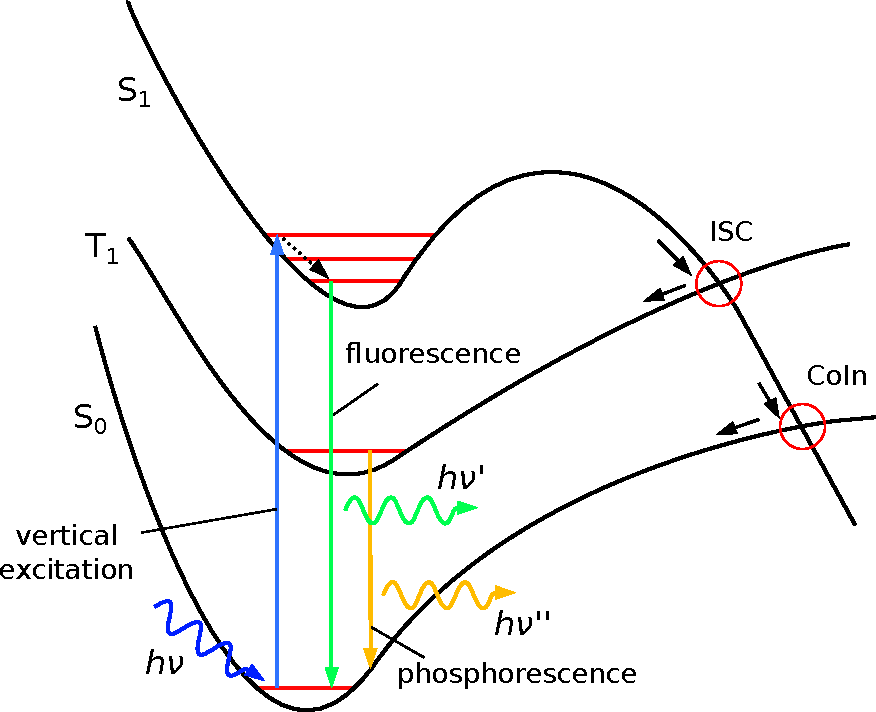
\includegraphics[scale=0.8]{Pics/PESEX}
\caption{Potential energy surface of a chemical system depicting the major pathways encountered in spectroscopy and photochemistry.}
\label{fig:PESEX}
\end{figure}

\section{Explicit Optimization of the Excited State Wave Function}

One of the conceptually simplest approaches for obtaining information on excited states is explicit optimization of the excited wave function. The excitation energy is then directly computed by taking the difference between the ground state energy and the energy of excited state $i$
\begin{equation}
E_{0\rightarrow i} = E_i - E_0 
\end{equation} 
\noindent Any ground state model discussed in the previous chapter can be used. This approach to excited states is known by different names, depending on which approximation is used. Generally, the Greek letter $\Delta$ is just prepended to the method name, giving $\Delta$SCF or $\Delta$HF for Hartree-Fock \cite{Bag1965,Deu1976,Amb2019}, $\Delta$KS (Kohn-Sham) or $\Delta$DFT for DFT \cite{Tri1999,Tak2003,Bes2009}, and so on. At the moment of writing, excitation energies are also routinely computed using $\Delta$MP$n$ \cite{Hol2011}, $\Delta$CI, $\Delta$MCSCF \cite{Sch2015} and $\Delta$CC \cite{Hol2011,Zhe2019}. From here on out, $\Delta$X will be used as an umbrella term to group all aforementioned terms. 

Despite the simplicity of the $\Delta$X methods, obtaining a solution to the KS or HF equations for higher energy states is non-trivial. By the variational principle, the SCF method finds the lowest energy solution. A HF type excited wave function may therefore collapse to that lowest energy solution during the SCF procedure (variational collapse). For small symmetric molecules, it is possible to converge excited states if they have a different spin multiplicity or spatial point group to the ground state. If the ground and excited state have the same symmetry however, this approach will not work. This technical difficulty was one of reasons why $\Delta$X methods never gained much ground compared to more sophisticated methods.

In 2008, Gilbert et al. \cite{Gil2008} proposed a modification the SCF procedure that prevents variational collapse, known as the \emph{maximum overlap method} (MOM). On each iteration, the new guess orbitals are obtained by diagonalization of the Fock matrix which is constructed using the old coefficients
\begin{equation}
\mbf{F}(\mbf{C}^{old})\mbf{C}^{new} = \mbf{S}\mbf{C}^{new}\epsilon
\end{equation}
\noindent At this step, it is possible to decide which of those new orbitals are actually occupied. Normally, the $n_{occ}$ eigenvectors with the lowest eigenvalues are chosen as the new occupied MOs. Alternatively, the MOM protocol chooses the set of new MOs that overlap most with the span of the old coefficients, by evaluating the overlap matrix
\begin{equation}
\mbf{O} = (\mbf{C}^{old})\pdg \mbf{C}
\end{equation}
\noindent The maximum overlap method has led to a renewed interest in the $\Delta$X methods in recent years, especially in the context of core excitations and ionizations. 

Adding to the above-mentioned technical difficulties, there are several other known criticisms. First, each excited state requires a separately optimized wave function, which may become a limiting factor. Second, the $\Delta$X methods assume that a transition can be represented by an excitation involving two orbitals. The separate optimization generally leads to the excited states being non-orthogonal, and there is considerable overlap between high and low energy states \cite{Dav1964,Dav1965,Gil2008}. $\Delta$X is therefore assumed to be only applicable to low-lying excited states. Third, the transition moments cannot be computed directly, but need to be evaluated using Fermi's Golden Rule \cite{Gro2008}. Furthermore, to allow a comparison with experimental XAS spectra, the calculated transition energies must be convoluted, for example by Gaussian functions, to 
account for the finite experimental resolution and  lifetime of the electron hole. Finally, using an unrestricted HF or KS formalism leads to spin contamination. A single excited state is not a pure singlet but a mixture of singlet and triplet state. Spin contamination can be alleviated by applying Ziegler's spin purification formula \cite{Zie1977}:

\begin{equation}
E_S = 2 E_{mixed} - E_T
\end{equation}

Despite these disadvantages, $\Delta$X is still an attractive and low-cost alternative to response and propagator methods.


\section{The Algebraic Diagrammatic Construction Method}

The algebraic diagrammatic construction (ADC) scheme is an excited state method originating from Green's functions \cite{Sch1982,Sch2018}. By diagrammatic perturbation expansion of electron propagators, ADC gives a hierarchy of methods which systematically converge to the exact solution (Full CI).  

\subsection{Many-Body Green's Function}

Many-Body Green's Functions (MBGFs) are powerful tools to treat electron correlation in quantum mechanics. They are more commonly encountered in (condensed matter) physics, for the modeling of strongly correlated systems such as metals or semi-conductors. MBGFs get their name from their building blocks: Green's functions (GFs). GFs, or \emph{correlation functions}, are special solutions to differential equations (DEQs).

Consider the inhomogeneous DEQ in one dimension:
\begin{equation}
\hat{D}_x y(x) = f(x)
\end{equation}
\noindent where $\hat{D}$ is a linear differential operator. The general solution can be divided into a \emph{homogeneous} and a \emph{special} part
\begin{equation}
y(x) = y_{hom}(x) + y_{spec}(x)
\end{equation}
\noindent where $y_{hom}$ is the solution to the homogeneous equation $\hat{D}y_{hom}(x)$ = 0. The special solution can be expressed in terms of GFs which are defined as the solution to the DEQ where the inhomogeneity is a Dirac function:
\begin{equation}
\hat{D}_x G(x,x') = \delta(x-x')
\end{equation}
\noindent A special solution can then be constructed by
\begin{equation}
y_{spec} = \int G(x,x')f(x') dx
\end{equation}
\noindent for any inhomogeneity $f(x)$. 

The Schrödinger equation is also a differential equation where the inhomogeneity takes the role of the external perturbation $V$
\begin{equation}
\left[ i\frac{\partial}{\partial t} + \frac{1}{2} \nabla^2 \right] \Psi(\mbf{r},t) = V(\mbf{r},t) \Psi(\mbf{r},t)
\end{equation}
\noindent The wave function may then be expressed by
\begin{equation}
\Psi(\mbf{r},t) = \int G(\mbf{r},t;\mbf{r}',t') \Psi
\end{equation}
\noindent The GF has the effect of \emph{propagating} the wave function from a given time and position to another time and space coordinate. GFs are therefore also known as \emph{propagators}.

The MBGFs form a hierarchy, in which the one-particle GFs are the lowest rank (Figure \ref{fig:PROP}). One-particle GFs can be used to extract information on 1-electron processes such as ionization and electron attachment. Two-particle GFs form the next step in the hierarchy, and allow to gain information on two-particle processes such as electron excitation (electron-hole) and two-electron ionization (electron-electron). 
\begin{figure}
\centering
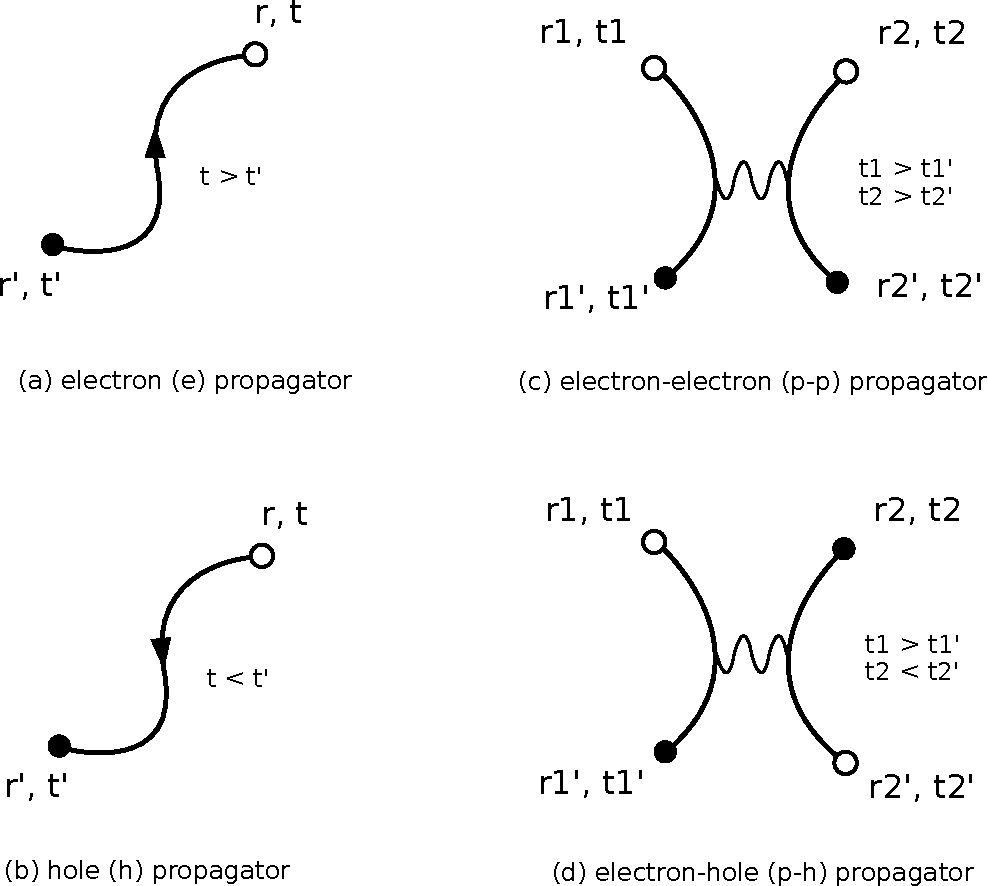
\includegraphics[scale=0.6]{Pics/PROP}
\caption{Hierarchy of Green's functions}
\label{fig:PROP}
\end{figure}

\subsubsection{One-electron Propagator}

To see how GFs can be used for excited state analysis, consider the 1-electron propagator in the time domain
\begin{equation}
G_{pq}(t,t') = - i\Theta(t-t') \sbra{\Psi_0} \hat{T}(a_p[t]a
_q\pdg[t']) \sket{\Psi_0}
\end{equation}
\noindent with $\Theta$ as the Heaviside step function, and the time-ordering operator 
\begin{equation}
\hat{T} = \left\lbrace \begin{matrix}
a_p[t] a_q\pdg[t'] \quad \textrm{for } t > t' \\
-a_q\pdg[t'] a_p[t] \quad \textrm{for } t < t'
\end{matrix}
\right.
\end{equation}
\noindent which plays the role of conserving symmetry with respect to time. It is useful to switch to the energy representation of the GF by Fourier transformation
\begin{equation}
G_{pq} (\omega) = \underbrace{ \sum_n \frac{
	\sbra{\Psi_0} c_p \sket{\Psi_n^{N+1}}			    \sbra{\Psi_n^{N+1}} c_q \pdg \sket{\Psi_0} 
}{
	\omega + E_0 - E_n^{N+1} + i \eta
}
}_{\text{$G^{+}(t,t')$}} + 
\underbrace{
\sum_n \frac{
	\sbra{\Psi_0} c_q \pdg \sket{\Psi_n^{N-1}}			    \sbra{\Psi_n^{N-1}} c_p \sket{\Psi_0}
}{
	\omega + E_n^{N-1} - E_0 - i \eta
}
}_{\text{$G^{-}(t,t')$}}
\end{equation}
\noindent also known as the spectral, energy or Lehmann representation. The superscripts $N+1$ and $N-1$ indicate the addition or removal of an electron form the $N$-electron wave function. The left-hand sum $G^{+}$ describes electron attachment and the right-hand term $G^{-}$ describes electron detachment (ionization). The singularities or \emph{poles} of the spectral representation give the $n$th electron affinity and ionization energy 
\begin{align}
A_n &= E_0 - E_n^{N+1} \\
I_n &= E_n^{N-1} - E_0
\end{align}
\noindent Moreover, the transition strengths (or pole strengths) are given by the spectroscopic factors 
\begin{equation}
x_p^{(n)} = \bra{\Psi_0 } c_p \ket{\Psi_n ^{N+1} }, \quad n \in \left\lbrace N + 1 \right\rbrace
\end{equation}
\begin{equation}
x_p^{(n)} = \bra{\Psi_n^{N-1} } c_p \ket{\Psi_0 }, \quad n \in \left\lbrace N - 1 \right\rbrace
\end{equation}
\noindent By analyzing the 1e-GF, it is therefore possible compute the 1-particle excitation spectrum. 

\subsubsection{Polarization Propagator}

A solution to the single-particle SEQ can be given directly by integrating the GFs. For many-electron systems however, one- and two-particle GFs are only building blocks for many-body propagators. The 1p and 2p GFs allow to introduce the particle-hole response function 
\begin{equation}
R_{pq,uv}(t_1,t_2;t_1',t_2') = G_{pq,uv}(t_1,t_2;t_1',t_2') - G_{pu}(t_1,t_1')G_{qv}(t_2,t_2')
\end{equation}
\noindent also known as the two-particle correlation function. It is the variational derivative of the 1p-GF with respect to an external perturbation $V(t_1,t_2)$, for example in the form of an incoming light quantum \cite{Bay1962}. Similarly to the 1p-GF, analyzing the ph response function gives information on the excited state. It can be evaluated directly via the Bethe-Salpeter equations \cite{Nam1950,Sal1951}, but their dependency on four time variables make them difficult to solve. Fortunately, the same information is already contained in the \emph{polarization propagator} defined by
\begin{equation}
\Pi(t,t') = \lim_{\substack{t_1 \rightarrow t_1'=t \\
t_2 \rightarrow t_2' = t'}} iR(t_1,t_2;t_1',t_2')
\end{equation}  
\noindent The spectral representation of $\Pi$ takes the form
\begin{equation}
\Pi _{p,q;r,s} = \underbrace{ \sum_{n \neq 0} \frac{ 
	\bra{\Psi_0} \hat{c}_q \pdg \hat{c}_p 		\ket{\Psi_n} \bra{\Psi_n} \hat{c}_r \pdg \hat{c}_s \ket{\Psi_0}
}{
	\omega - (E_n - E_0) + i \eta
} }_\text{$\Pi _+(\omega)$} + \underbrace{ \sum_{n \neq 0} \frac{ 
	\bra{\Psi_0} \hat{c}_r \pdg \hat{c}_s \ket{\Psi_n} \bra{\Psi_n} \hat{c}_q \pdg \hat{c}_p \ket{\Psi_0}
}{
	- \omega - (E_n - E_0) + i \eta
} }_\text{$\Pi _-(\omega)$}
\label{eq:POLPROP}
\end{equation}
\noindent Here, the poles correspond to the excitation energies $\omega_n = E_n - E_0$ and the spectroscopic factors give the transition strengths. The polarization propagator is therefore all one needs to evaluate absorption or emission spectra of molecules. The left and right hand terms are related by
\begin{equation}
\Pi(-\omega)_{+}\pdg = \Pi_{-}(\omega)
\end{equation}

Up to this point, the exact wave function was used in the expression for the propagators. To actually be able to compute the propagators, approximations need to be applied. There are a couple of choices. Coupled cluster linear response theory inserts the CC ansatz for the wave function and explicitly evaluates expressions for the polarization propagator truncated to a given level of excitations (LR-CCSD, LR-CCSDT etc.).

Alternatively, the polarization propagator may be approached using perturbation theory.

\subsubsection{Diagrammatic Perturbation}

Similarly to the wave function in RSPT, the polarization propagator can be expanded as
\begin{equation}
\Pi = \Pi^{(0)} + \Pi^({1}) + \Pi^{(2)} + \ldots
\label{eq:PERTPOLPROP}
\end{equation}
\noindent The same partitioning of the Hamiltonian is used as in RSPT
\begin{equation}
\hat{H} = \hat{H}_0 + \hat{U}
\end{equation}
\noindent with the expressions for the wave functions and their energies given in Equations ... and ... 

One may then evaluate the series \ref{eq:PERTPOLPROP} using either Rayleigh-Schrödinger perturbation theory or the Gell-Mann Low theorem \cite{Sch2018} to obtain master equations for $\Pi^{(n)}$. However, these equations are very tedious to solve, even more so than for M{\o}ller Plesset, due to the rapidly increasing number of nested terms for higher $n$. For this reason, diagrams were introduced to better keep track of the contributions at a given level. 

Diagrams were originally conceived by Feynman, and are a pictorial representation of mathematical expressions for particle interactions. Over the years, many different types of diagrams were proposed, such as Goldstone, Abrikosov or Hugenholtz diagrams. Each type has its own set of rules on how to construct them and translate them into formulas for a given problem. There is no formal proof: Feynman first worked out the rules by trial and error \cite{Fey1966}, and later refined the model.

% Bay1962 https://journals.aps.org/pr/abstract/10.1103/PhysRev.127.1391
% Sal1951 E. E. Salpeter and H. A. Bethe, Phys. Rev. 84, 1232 (1951)
% Fey1966 https://science.sciencemag.org/content/153/3737/699

Figure ... shows the Feynman diagrams (in Abrikosov notation) for the polarization propagator up to second order. Each line represents a free particle (electron or hole). Lines with the arrow pointing up are also known as particle lines, while those with the arrow pointing down are known as hole lines. Here, the particle lines represent the time evolution of the electron between $t$ and $t'$. The perturbation $\hat{V}$ is represented by dots in the diagrams, with the total number of dots indicating the perturbation order of the diagram. Each dot contributes a factor of $V_{rs[r's']}=\sbra{rs}\hat{V}\sket{r's'} - \sbra{rs}\hat{V}\sket{s'r'}$ to the mathematical expression of the diagram, where $r,s$ and $r',s'$ are incoming and outgoing fermion lines. Each vertex contributes a free one-particle Green's function $G^0_x(t,t')$. Further rules need to be applied to get the correct sign factors from the direction of the lines. As an example, consider the first order expression of the polarization propagator
\begin{equation}
\Pi^{(1)}_{rs,r's'}(t,t') = \sum_{-\infty}^{\infty} \hat{V}_{rs[r's']}  G^{0}_r(t,t_1) G^0_s(t_1,t) G^0_{r'}(t_1,t') G_{s'}^0(t',t_1) dt_1
\label{eq:SPECTRALORDER1}
\end{equation}
\noindent Equation \ref{eq:SPECTRALORDER1} can then be transformed to the energy representation. Alternatively, Goldstone diagrams can be used where the set of rules directly gives the spectral instead of the time representation. 

\begin{figure}
\centering
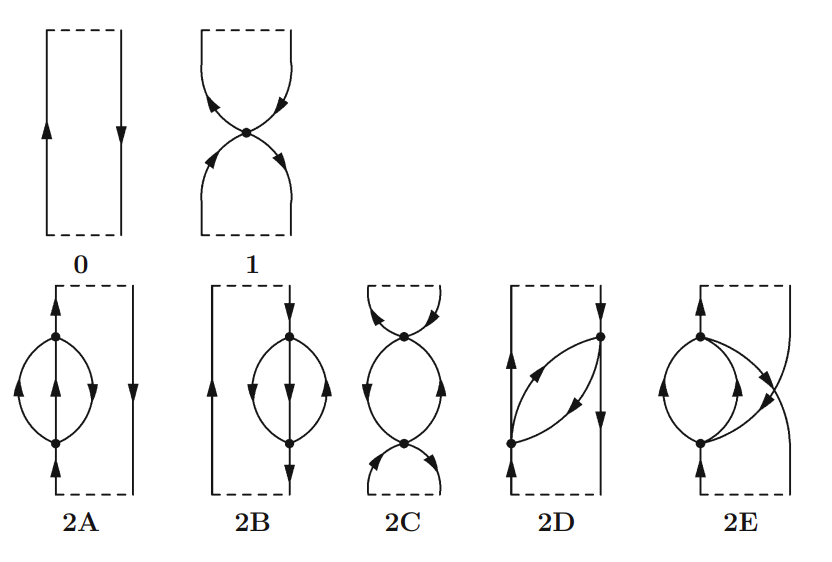
\includegraphics[scale=0.4]{Pics/POLPROP.png}
\label{fig:POLPROP}
\caption{Feynman diagrams in Abrikosov notation for the polarization propagator through second order. Taken from \cite{Sch2018}.}
\end{figure}

\subsection{The ADC scheme}

The polarization propagator cannot be directly "measured". To establish a bridge between theory and experiments, the \emph{transition function} is introduced as
\begin{equation}
T(\omega) = D\pdg \boldsymbol{\Pi}_{+} D 
\end{equation}
\noindent where $\hat{D}$ is an arbitrary operator. The quantity measured during experiments is the \emph{spectral function}, given by
\begin{equation}
f(\omega) = \frac{1}{\pi}Im\{T(\omega)\}
\end{equation}
In the algebraic diagrammatic construction method, the transition function is reformulated as
\begin{equation}
T(\omega) = \mbf{F}\pdg \mbf{\Gamma}(\omega) \mbf{F}
\end{equation}
\noindent where $\mbf{F}$ are the modified transition moments and the non-diagonal matrix $\mbf{\Gamma}$ is given by
\begin{equation}
\mbf{\Gamma}(\omega) = \left[ \omega \mbf{1} - (\mbf{K} + \mbf{C}) \right] = \left[ \omega \mbf{1} - \mbf{M} \right]
\end{equation}
\noindent with the ADC matrix $\mbf{M}$. Writing the transition function, the modified transition moments and $\mbf{M}$ as a perturbation expansion
\begin{align}
T(\omega) &= \sum_{n=0}^{\infty} T^{(n)}(\omega) = \sum_{n=0}^{\infty} D\pdg \boldsymbol{\Pi}_{+}^{(n)} D
\mbf{F} &= \sum_{n=0}^{\infty} \mbf{F}^{(n)} \\
\mbf{M} &= \mbf{K} + \sum_{n=1}^{\infty} \mbf{C}^{(n)}
\end{align} 
\noindent the $n$th order approximations to the transition function read
\begin{align}
T^{(0)}(\omega) &= \mathbf{F}^{(0)\dagger} \left[ \omega \mathbf{1} - \mathbf{K} \right]^{-1} \mathbf{F}^{(0)} \\
\begin{split}
T^{(1)}(\omega) &= \mathbf{F}^{(0)\dagger} \left[ \omega \mathbf{1} - \mathbf{K} \right]^{-1} \mathbf{C}^{(1)} \left[ \omega \mathbf{1} - \mathbf{K} \right]^{-1} \mathbf{F}^{(0)} + \mathbf{F}^{(1)\dagger} \left[ \omega \mathbf{1} - \mathbf{K} \right]^{-1} \mathbf{F}^{(0)} \\
&+ \mathbf{F}^{(0)\dagger} \left[ \omega \mathbf{1} - \mathbf{K} \right]^{-1} \mathbf{F}^{(1)} 
\end{split} 
\\
\begin{split}
T^{(2)}(\omega) &= \mathbf{F}^{(1)\dagger} \left[ \omega \mathbf{1} - \mathbf{K} \right]^{-1} \mathbf{F}^{(1)} + \mathbf{F}^{(0)\dagger} \left[ \omega \mathbf{1} - \mathbf{K} \right]^{-1} \mathbf{C}^{(2)} \left[ \omega \mathbf{1} - \mathbf{K} \right]^{-1} \mathbf{F}^{(0)} \\
&+ \mathbf{F}^{(0)\dagger} \left[ \omega \mathbf{1} - \mathbf{K} \right]^{-1} \mathbf{C}^{(1)} \left[ \omega \mathbf{1} - \mathbf{K} \right]^{-1} \mathbf{C}^{(1)} \left[ \omega \mathbf{1} - \mathbf{K} \right]^{-1} \mathbf{F}^{(0)} \\
&+ \mathbf{F}^{(1)\dagger} \left[ \omega \mathbf{1} - \mathbf{K} \right]^{-1} \mathbf{C}^{(1)} \left[ \omega \mathbf{1} - \mathbf{K} \right]^{-1} \mathbf{F}^{(0)} \\
&+ \mathbf{F}^{(0)\dagger} \left[ \omega \mathbf{1} - \mathbf{K} \right]^{-1} \mathbf{C}^{(1)} \left[ \omega \mathbf{1} - \mathbf{K} \right]^{-1} \mathbf{F}^{(1)}
\end{split}
\end{align}
\noindent By comparing the above $n$th order expression of the transition operator $T(\omega)^{(n)}$ with the mathematical expression of $\mbf{D}\pdg \mbf{\Pi}(\omega) \mbf{D}$ derived using the diagrammatic perturbation of the polarization propagator, algebraic expressions can be \emph{constructed} for the transition moments $\mbf{F}$, and the matrices $\mbf{K}$ and $\mbf{C}$, hence the name algebraic diagrammatic construction.

\subsection{Structure of the ADC matrix}

At its core, ADC reduces to the eigenvalue problem
\begin{equation}
\mbf{M}\mbf{X} = \mbf{X}\boldsymbol{\Omega}
\label{eq:ADCEVAL}
\end{equation}
\noindent The solution gives the vertical excitation energies $\boldsymbol{\Omega}$ and the eigenvectors $\mbf{X}$. Figure \ref{fig:ADCMAT} shows the structure of the ADC matrix $\mbf{M}$ up to third order. Each second level $n$ adds an additional higher excitation manifold to the matrix. ADC(0) and ADC(1) include only singles, while ADC(2) and ADC(3) also include doubles.

The ADC(0) matrix contains only the Hartree-Fock orbital energy differences:
\begin{equation}
M^{(0)}_{ia,jb} = K_{ia,jb} = \delta_{ij}\delta_{ab} (\eps_i - \eps_a) 
\end{equation}
\noindent The ADC(1) matrix adds the first order expression for $\mbf{C}$, and is identical to the CIS matrix:
\begin{equation}
M^{(1)}_{ia,jb} = K_{ia,jb} + C_{ia,jb}^{(1)} = \delta_{ij}\delta_{ab} (\eps_i - \eps_a) - \sbra{ij}\sket{ab}
\end{equation} 
\noindent The ADC(2) matrix has additional second order contributions to the p-h block, and approximates the 2h-1p, 1h-2p to first order and the 2p-2h to zeroth order. 
\begin{align}
C_{ijab}^{(2)} &= C_{ijab}^{(2)A} + C_{ijab}^{(2)B} + C_{ijab}^{(2)C} 
\\
C_{ia,jkcl}^{(1)} &= \sbra{kl} \sket{id} \delta_{ac} - \sbra{kl} \sket{ic} \delta_{ad} - \sbra{al} \sket{cd} \delta_{ik} + \sbra{ak} \sket{cd} \delta_{il} 
\\
C_{iajb,kc}^{(1)} &= \sbra{kb} \sket{ij} \delta_{ac} - \sbra{ka} \sket{ij} \delta_{bc} - \bra{ab} \sket{cj} \delta_{ik} + \sbra{ab} \sket{ci} \delta_{jk} 
\\
K_{iajb,kcld} &= (\epsilon_a - \epsilon_i + \epsilon_b - \epsilon_j) \delta_{ac} \delta_{bd} \delta_{ik} \delta_{jl} 
\end{align}

\noindent with

\begin{align}
C_{ijab}^{(2)A} &= \frac{1}{4} \delta_{ij} \sum_{ckl} \left[  \hat{t}_{ackl} \bra{kl} \sket{bc}  +  \bra{ac} \ket{kl} \hat{t}_{klbc}\right] \\
C_{ijab}^{(2)B} &= \frac{1}{4} \delta_{ab} \sum_{cdk} \left[ \hat{t}_{cdik} \bra{jk} \ket{cd} + \bra{cd} \ket{ik} \hat{t}_{jkcd} \right] \\
C_{ijab}^{(2)C} &= - \frac{1}{2} \sum_{ck} \left[ \hat{t}_{acik}  \bra{jk} \ket{bc} + \bra{ac} \ket{ik} \hat{t}_{jkbc} \right] 
\end{align}

and the anti-symmetrized MP2 amplitudes

\begin{equation}
\hat{t}_{ijab} = \frac{\sbra{ij}\sket{ab}}{\eps_a + \eps_b - \eps_i - \eps_j}
\end{equation}

\begin{figure}
\centering
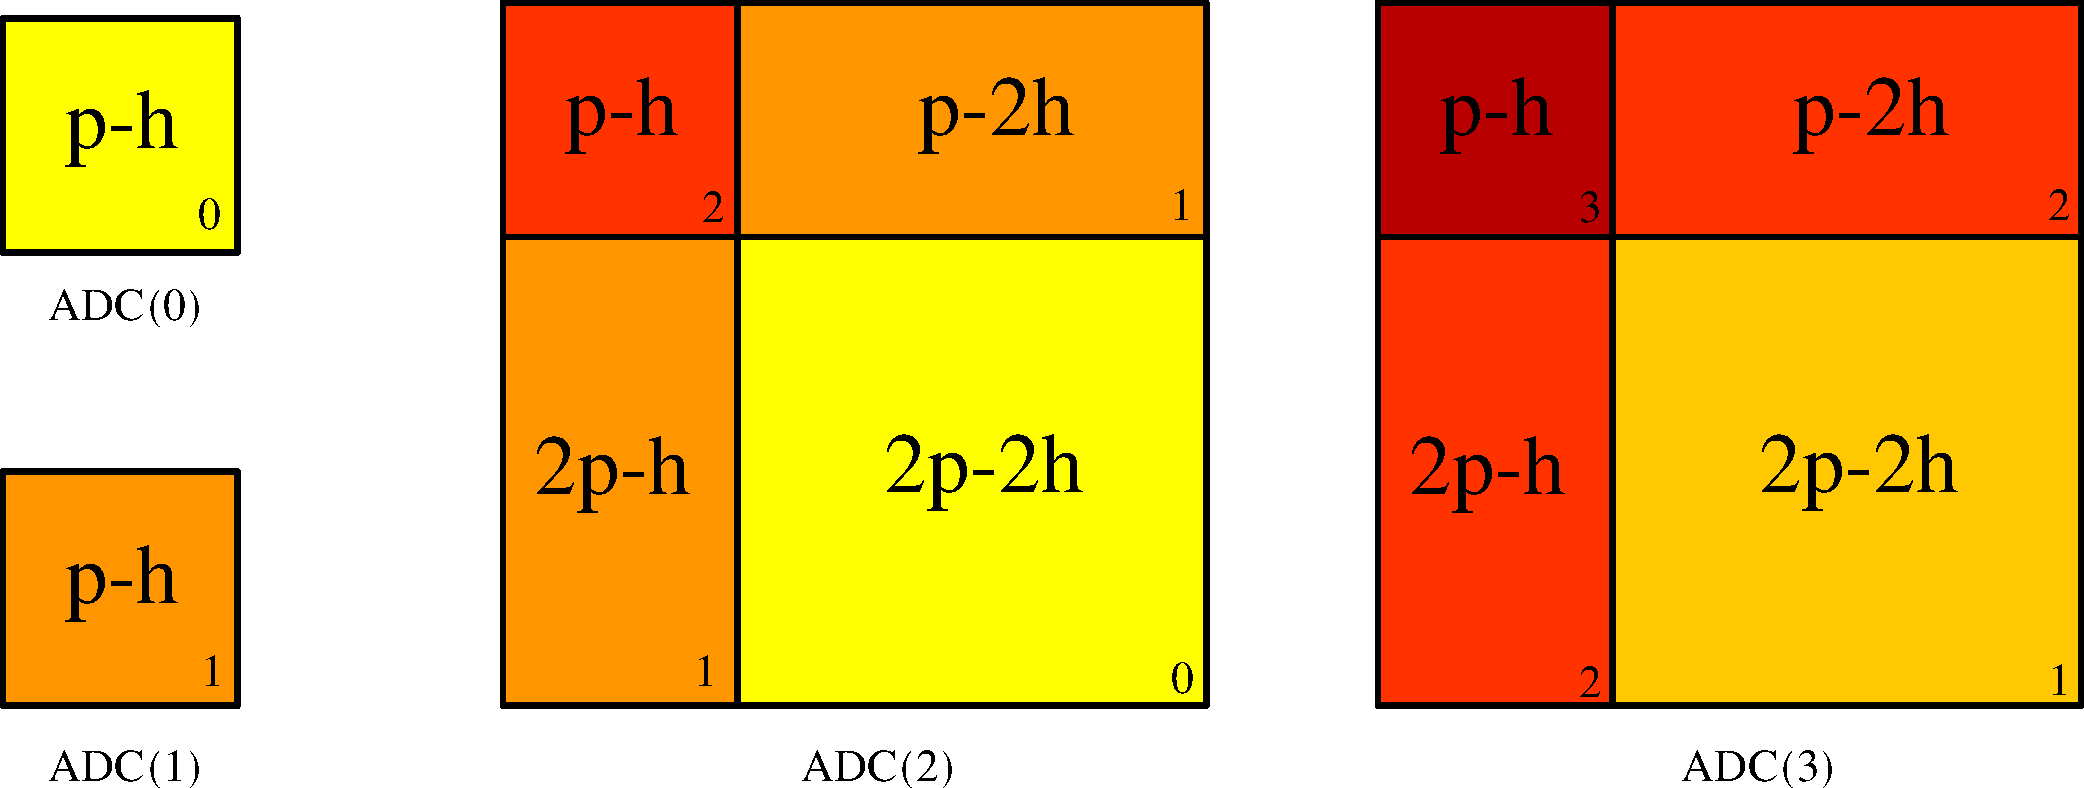
\includegraphics[scale=0.4]{Pics/ADCMAT2}
\caption{Structure of the ADC matrix from zeroth through third order. The number in each block indicates the perturbation order.}
\label{fig:ADCMAT}
\end{figure}

Approximating the 2p-2h block to first order in the ADC(2) matrix, i.e. swapping the 2p-2h block with the one from the ADC(3) matrix, gives the so-called extended ADC(2) scheme (ADC(2)-x). It is an \emph{ad-hoc} extension without rigorous theoretical justification \cite{Tro1995}.  

\subsection{Solving the Eigenvalue Problem \label{sec:ADC_DAV}}

The eigenvalue problem \ref{eq:ADCEVAL} is typically solved using the Davidson procedure to extract the first few eigenvalues, analogous to configuration interaction. Rather than constructing the whole ADC matrix, closed expressions are derived for the matrix-vector products of the different blocks with a general trial vector $\mbf{u}$. For computational considerations, the matrix-vector product is split into its individual components which are then multiplied by the sub-blocks of the ADC matrix. In the case of ADC(2) and ADC(3), the components are limited to singles and doubles contributions:
\begin{align}
r_{ia} &= A_{ia,jb} u_{jb} + A_{ia,jbkc} u_{jbkc} \\
r_{iajb} &= A_{iajb,kc} u_{kc} + A_{iajb,kcld} u_{kcld} 
\end{align}

While the Davidson procedure allows to circumvent storing the whole ADC matrix, the storage of the trial vectors can still be a major memory bottle-neck for ADC(2) and beyond. At second and third order, the doubles part of the vectors scale with $n_{occ}^2n_{vir}^2$, and take up as much space as the MP2 amplitudes. As the Davidson subspace grows, so does the number of trial vectors. Techniques such as \emph{subspace collapse} (Section \ref{sec:DAV}) impose a maximum to the number of trial vectors held in memory, which helps to better estimate the total storage size needed by an ADC calculation, although it increases the total number of iterations to convergence.

An alternative technique to reduce the memory footprint of the Davidson diagonalization is \emph{doubles-folding}. Consider the doubles part of the MVP which is computed as
\begin{align}
r_{iajb} &= A_{iajb,kc} u_{kc} + A_{iajb,kcld} u_{kcld} = \omega u_{iajb}
\end{align}
\noindent By refactoring the above expression, the doubles component of $\mbf{u}$ can be reformulated in terms of its singles component as
\begin{equation}
u_{iajb} = \frac{A_{iajb,kc} u_{kc}}{\omega - A_{iajb,iajb}} 
\label{eq:DS}
\end{equation}
\noindent This technique is limited to ADC(2) only, where the doubles-doubles block is diagonal. Substituting \ref{eq:DS} into the singles expression of the MVP, and using the explicit formulas for the doubles-doubles block gives
\begin{equation}
r_{ia} = A_{ia,jb} u_{jb} + A_{ia,jbkc} \frac{A_{jbkc,ld} u_{ld}}{\omega - \eps_j - \eps_k + \eps_b + \eps_c} 
\end{equation}
\noindent The doubles part of the MVP is computed on-the-fly and does not need to be explicitly stored, reducing the overall memory requirements of the Davidson diagonalization to $n_{occ}n_{vir}$. Doubles-folding corresponds to a multiplication of the singles vectors with an \emph{effective} ADC matrix which depends on the eigenvalue $\omega$
\begin{equation}
\mbf{r}_{\mu_1} = \mbf{A}(\omega)_{\mu_1\nu_1} \mbf{u}_{\nu_1} 
\end{equation}
\noindent One drawback of doubles-folding is that a modified Davidson procedure is necessary to solve this \emph{pseudo} eigenvalue problem (see \ref{seq:DAV}) due to the dependence on the excitation energy $\omega$.

\subsection{Intermediate states}

An alternative route to deriving the ADC working equations is via the intermediate state representation 
\cite{Sch1991,Sch2004,Kni2012}.
%(refs 55, 63, 77, 78 Andreas). 

The previous derivation showed that the eigenvalues of the ADC matrix $\mbf{M}$ correspond to the excitation energies, and that it can be expanded in a perturbation series. These features suggest that $\mbf{M}$ is a representation of the energy-shifted Hamiltonian
\begin{equation}
\mbf{M} = \mbf{H} - E_0
\end{equation}
\noindent with the matrix elements 
\begin{equation}
M_{IJ} = -\sbra{\tPsi_I} \hat{H} - E_0 \sket{\tPsi_J}
\label{eq:ISMATELE}
\end{equation}
\noindent Here, the space of the shifted Hamiltonian is spanned by a set of \emph{intermediate states}. Starting from the set of \emph{correlated excited} (CE) states
\begin{equation}
\sket{\Psi^{\#}_I} = \hat{C}_I \sket{\Psi_0} 
\end{equation}
\noindent with the excitation operators
\begin{equation}
\{\hat{C}_I\} = \{ a_a\pdg a_i; a_b\pdg a_j c_a\pdg c_i; \ldots \}
\end{equation}
\noindent the intermediate states are obtained by a step-wise Gram-Schmidt orthogonalization of the CE states. The ground state $\sket{\Psi_0}$ is approximated by MPPT. Constructing the intermediate states from the MP$n$ ground state wave function and evaluating the matrix elements according to \ref{eq:ISMATELE} gives the $n$th order ADC matrix. For this reason, ADC is also known as "excited state method for M{\o}ller-Plesset". 

\subsection{Spin-Opposite Scaled ADC \label{sec:SOSADC}}

The spin-opposite scaling method previously applied to MP2 and CC2 can be expanded to ADC(2) as well.    There are two version of SOS-ADC(2): the version which will be referred to as "standard" SOS-ADC(2) derived from the SOS-CC2 linear response equations \cite{Win2011}, and ISR-SOS-ADC(2) derived from SOS-MP2 using the intermediate state representation \cite{Kra2013}. Standard SOS-ADC(2) introduces the following modifications to the ADC(2) matrix:
\begin{enumerate}
\item The same-spin contributions of antisymmetrized MP2 amplitudes are ignored, and the opposite-spin components are scaled up:
\begin{equation}
\hat{t}_{IAJB}^{SOS} = c_{os} \hat{t}_{IAJB} \left( 1 - \delta _{\sigma (I) \sigma (J)} \right)
\label{eq:SOSAMPLITUDES}
\end{equation}
where $\sigma (x)$ gives the spin of $x$, and with the amplitudes given by
\begin{equation}
\hat{t}_{IAJB} = \frac{\bra{IJ}{}\ket{AB}}{\epsilon_A + \epsilon_B - \epsilon_I - \epsilon_J}
\end{equation}
\item All same-spin entries of the 2p-1h and 1p-2h blocks of the ADC(2) matrix are deleted ($\alpha\alpha\alpha\alpha$ and $\beta\beta\beta\beta$), and the  remaining blocks are scaled up:
\begin{equation}
M_{ia,kcld} = c_{osc} \left( \bra{kl}{}\ket{id} \gd_{ac} - \bra{kl}{}\ket{ic} \delta_{ac} - \bra{al}{}\ket{cd} \delta_{ik} + \bra{ak}{}\ket{cd} \delta_{il} \right) \left( 1 - \delta_{\sigma (k) \sigma (l)} \right)
\end{equation}
\begin{equation}
M_{iajb,kc} = c_{osc} \left( \bk{kb}{ij} \gd_{ac} - \bk{ka}{ij} \gd_{bc} - \bk{ab}{cj} \gd_{ik} + \bk{ab}{ci} \gd_{jk} \right) \left( 1 - \gd_{\gs (i) \gs (j)} \right)
\end{equation}
\noindent where $c_{osc}$ is the opposite-spin coupling constant, typically set to 1.15 \cite{Kra2013} or 1.17 (diss).
\end{enumerate}

\noindent For open-shell molecules, this drastically reduces the size of the matrix, reducing the prefactor of the method. By applying density fitting, the total scaling can be further reduced by an order of magnitude \cite{Win2011}.

ISR-SOS-ADC(2) does not modify the off-diagonal blocks of the ADC(2) and only replaces the amplitudes as in Equation \ref{eq:SOSAMPLITUDES}, and therefore offers no substantial improvement. 

% 85 https://www.sciencedirect.com/science/article/abs/pii/S030101041100423X
% 86 https://aip.scitation.org/doi/abs/10.1063/1.4776675

\FloatBarrier

\subsection{Performance and Accuracy}

Table \ref{tab:ADCSTATS} lists the formal scaling, mean errors and standard deviation of excitation energies for the ADC($n$) methods. ADC(2), similarly to MP2, offers an economical way of computing excited state properties compared to other excited state methods with similar accuracy. ADC(2)-x and ADC(3) have the same scaling factor, but ADC(2)-x has a lower prefactor.  

The ADC methods offer high accuracy and high precision on the order of a few tenths of eV . The SOS method can significantly reduce the errors, but it should be kept in mind that the spin coefficients were fitted to the benchmark set, and similar accuracy is not guaranteed for other systems.

\begin{table}[h]
\centering
\begin{tabular}{llll}
\hline
Method & Scaling & Singlets & Triplets \\ \hline
ADC(2) & $\ccpx{5}$ & 0.22 $\pm$ 0.38 (62) & 0.12 $\pm$ 0.16 (62) \\
SOS-ADC(2) & $\ccpx{5}$ & 0.00 $\pm$ 0.15 (87) & 0.06 $\pm$ 0.10 (87) \\
ADC(2)-x & $\ccpx{6}$ & -0.70 $\pm$ 0.37 (62) & -0.55 $\pm$ 0.20 (62) \\
SOS-ADC(2)-x & $\ccpx{6}$ & -0.11 $\pm$ 0.18 (87) & -0.04 $\pm$ 0.12 (87) \\
ADC(3) & $\ccpx{6}$ & 0.12 $\pm$ 0.28 (64) & -0.18 $\pm$ 0.16 (64) \\ \hline  
\end{tabular}
\caption{Mean absolute errors (MAE) and deviations (in eV) for closed-shell molecules at various levels of theory. $^a$ \cite{Har2014}, $^b$ \cite{Kra2013}, $^c$ \cite{Tro2006}}
\label{tab:ADCSTATS}
\end{table}

\section{Response Theory}

Response theory is a popular tool similar to propagators that provides methods for computing the response of a molecule to an external, time-dependent perturbation, such as an electromagnetic field. It can be applied to different levels of theory, such as Hartree-Fock, DFT or Coupled Cluster, to gain information on various excited state properties.

\subsection{Exact Response Theory}

Consider a molecular system described by the time-independent Hamiltonian $\hat{H}_0$ with eigenfunctions $\ket{\Psi_0}$ exposed to
an external perturbation $\hat{V}$ given by \cite{Koc1990}
\begin{equation}
\hat{V}(t) = \int_{-\infty}^{\infty} \hat{V}^{\omega} e^{i\omega t  } d\omega
\end{equation}
\noindent where $\hat{V}^{\omega}$ is the representation of the external perturbation in the frequency domain, and $\epsilon$ is a real positive infinitesimal. It has the role of slowly "switching on" the perturbation as time progresses. For $t\rightarrow -\infty$, the perturbation is zero, and at $t \rightarrow \infty$, the perturbation is fully applied. This slow gradual switching makes sure that the process is \emph{adiabatic}.

The time-dependent wave function may be expanded in orders of the perturbation $\hat{V}(t)$ as
\begin{equation}
\sket{\Psi (t)} = \sket{\Psi_0} + \sket{\Psi^{(1)}(t)} + \sket{\Psi^{(2)}(t)} + \ldots
\end{equation}
\noindent which can be determined using Ehrenfest's theorem. Using this wave function expansion, the expectation value of a time-independent operator $\hat{A}$ reads
\begin{equation}
\begin{split}
\sbra{\Psi (t)} \hat{A} \sket{\Psi (t)} = & \sbra{\Psi_0} \hat{A} \sket{\Psi_0} + \int_{-\infty}^{\infty} 
\underbrace{ \langle\langle \hat{A}; \hat{V}^{\omega_1}
\rangle\rangle}_{\text{linear response}} 
e^{(-i\omega_1 + \eps)t} d\omega_1 \\
&+ \frac{1}{2} \int_{-\infty}^{\infty} \int_{-\infty}^{\infty}
\underbrace{ \langle\langle \hat{A}; \hat{V}^{\omega_1},\hat{V}^{\omega_2} \rangle\rangle 
}_{\text{quadratic reponse}}
e^{-i(\omega_1+\omega_2) + 2\eps)t} d\omega_1 d\omega_2  + \ldots
\end{split}
\label{eq:TIMEEXP}
\end{equation}

\noindent The expansion coefficients $\langle\langle \hat{A}; \cdot \rangle\rangle$ are known as \emph{response functions}. Different orders (linear, quadratic...) describe different processes. The linear response function may be used to describe single-photon absorption and polarizability, while the quadratic response function is needed to describe two-photon absorption and hyperpolarizability. 

The spectral representation of the linear response function takes the form
\begin{equation}
\langle\langle \hat{A}; \hat{B}
\rangle\rangle = \sum_k \frac{
	\sbra{\Psi_0}\hat{A}\sket{\Psi_k} \sbra{\Psi_k} \hat{B} \sket{\Psi_0}
}{
	\omega - E_n + E_0
} - \frac{ 
	\sbra{\Psi_0}\hat{B}\sket{\Psi_k} \sbra{\Psi_k} \hat{A} \sket{\Psi_0}
}{
	\omega + E_n - E_0
}
\end{equation}

\noindent and can be analyzed similarly to the polarization propagator: the poles of the function give the excitation energy
\begin{equation}
\omega_i = E_i - E_0
\end{equation}
and the residues give information about the transition moments 
\begin{equation}
\lim_{\omega \rightarrow  \omega_i} (\omega - \omega_i) \langle\langle \hat{A}; \hat{B} \rangle \rangle = \sbra{\Psi_0}\hat{A}\sket{\Psi_i} \sbra{\Psi_i} \hat{B} \sket{\Psi_0}
\end{equation}
for the $i$th excited state. The linear response function and the polarization propagator are related by \cite{Sch2018}
\begin{equation}
\langle\langle \hat{A}; \hat{B}
\rangle\rangle = \sum_{rsr's'} A_{rs} \mbf{\Pi} B_{r's'}
\end{equation}

The expressions for response functions are exact, and need to be evaluated by introducing approximations. Similar to the ADC scheme, finding the poles and residues of the response function ultimately reduces to an eigenvalue problem of the form
\begin{equation}
\mbf{A}\mbf{v} = \mbf{v}\mbf{\Omega}
\end{equation}
\noindent where $\mbf{A}$ can be symmetric (HF,DFT) or non-symmetric (CC).

\subsection{Time-Dependent Hartree-Fock}

There are many different routes for deriving the expressions for the matrix elements of $\mbf{A}$ for linear response time-dependent Hartree-Fock (TDHF) (cf. \ref{Dre2005}), which all lead to the same eigenvalue problem given by 
\begin{equation}
\begin{bmatrix}
\mbf{A} & \mbf{B} \\
\mbf{B}^* & \mbf{A}^* 
\end{bmatrix} 
\begin{bmatrix}
\mbf{X} \\
\mbf{Y} 
\end{bmatrix}
%= 
%\begin{bmatrix}
%\sbra{HF} \left[ \hat{q},\left[ \hat{H}_0, \hat{q}\pdg \right]\right] \sket{HF} & \sbra{HF} \left[ \hat{q},\left[ \hat{H}_0, \hat{q} \right] \right] \sket{HF}\\
%\sbra{HF} \left[ \hat{q}\pdg,\left[ \hat{H}_0, \hat{q}\pdg \right]\right] \sket{HF} & \sbra{HF} \left[ \hat{q}\pdg,\left[ \hat{H}_0, \hat{q} \right]\right] \sket{HF}
%\end{bmatrix}
= 
\omega 
\begin{bmatrix}
1 & 0 \\
0 & -1
\end{bmatrix}
\begin{bmatrix}
\mbf{X} \\
\mbf{Y} 
\end{bmatrix}
\label{eq:TDSCF}
\end{equation}
\noindent where $\mbf{A}$ is the matrix of single excitations, and $\mbf{B}$ couples the excitations with the de-excitations. The matrix elements are given by
\begin{align}
A_{IA,JB} &= \delta_{IA,JB} (\eps_A - \eps_I) + \sket{IJ}{AB} \\
B_{IA,JB} &= \sket{IJ}{AB}
\end{align}
\noindent Setting the coupling block $\mbf{B}$ to zero, the TDHF equations reduce to the CIS equations. Even if TDHF can therefore be seen as an extension to CIS, it does not give a considerable improvement. Over the years, it has fallen into disuse.

Linear response TDHF is equivalent to the \emph{random phase approximation}. 

% 2 McWeeny, R.; Sutcliffe, B. T. Methods of Molecular Quantum Mechanics; Academic Press: London, 1969
% Fetter, A. L.; Walecka, J. D. Quantum Theory of Many-Particle Systems; McGraw-Hill: New York, 1971
% Thouless, D. J. The Quantum Mechanics of Many Body Systems; Academic Press: New York, 1972.
% Dreuw, Andreas; Head-Gordon, Martin (2005). Single-Reference ab Initio Methods for the Calculation of Excited States of Large Molecules. , 105(11), 4009–4037.         doi:10.1021/cr0505627     

\subsection{Time-Dependent DFT}

The foundations of time-dependent DFT  will not be discussed here. The reader is referred to \cite{Dre2005} and references therein for more details. 

The TDDFT linear response equations are similar in structure to TDHF, reducing to the same eigenvalue problem \ref{eq:TDSCF}, with two different blocks $\mbf{A}$ and $\mbf{B}$ given by
\begin{align}
A_{IA,JB} &= \delta_{IA,JB} (\eps_A - \eps_I) + \sbraket{IJ}{AB} +  \sbra{IJ}\hat{f}_{xc} \sket{AB}  \\
B_{IA,JB} &= \sbraket{IJ}{AB} + \sbra{IJ}\hat{f}_{xc} \sket{AB}
\end{align}
\noindent Here, the exchange contributions are replaced by the so-called \emph{xc kernel}. In the adiabatic local density approximation (ALDA), the time dependent xc kernel is substituted by a time-independent kernel 
\begin{equation}
\sbra{IJ}\hat{f}_{xc} \sket{AB} = \int \phi^*_i(\mbf{r}) \phi_j(\mbf{r}') \frac{\partial^2 E_{xc}}{\partial\rho(\mbf{r})\rho(\mbf{r}')} \phi_a (\mbf{r}) \phi_b^*(\mbf{r}')
\end{equation}
\noindent which allows the use of standard xc functionals for the ground state. 

Since its introduction, TDDFT has evolved to become the most prominent method for computing excited state energies and transition moments. It has a computational cost on the same order as CIS, with an error of $\approx$ 0.3 eV \cite{Lau2013} for low-lying valence states. However TDDFT is not a panacea: excitation energies for Rydberg states, valence states of molecules with extended $\pi$-systems, doubly excited states and charge-transfer states exhibit errors on the order of several eV.

% Dreuw, Andreas; Head-Gordon, Martin (2005). Single-Reference ab Initio Methods for the Calculation of Excited States of Large Molecules. , 105(11), 4009–4037.         doi:10.1021/cr0505627     

% A. D. Laurent and D. Jacquemin, Int. J. Quantum Chem. , 2019 (2013)

\subsection{Coupled Cluster}

The derivation of the coupled cluster response equations is again a very lengthy and complex process \cite{Koc1990,Chr1998}. The most important steps will be summarized in this section.

For a molecular system in the presence of a static external perturbation, such as a constant electric or magnetic field with strength parameter $\lambda$, the Hellmann-Feynman theorem relates the expectation value of $\hat{X}_{\lambda}$ to the energy derivative by
\begin{equation}
\frac{\partial E}{\partial \lambda_x} = \sbra{\Psi}\frac{\partial \hat{H}}{\partial \lambda_x} \sket{\Psi} = \sbra{\Psi}\hat{X} \sket{\Psi}
\label{eq:HELLFEYN}
\end{equation}
\noindent By perturbation expansion of $\hat{X}$, the $n$th order property can then be related to the $n$th order derivative of the wave function energy, which is in most cases is more readily derived than the expectation value. For time-dependent perturbations, the theorem can be reformulated as 
\begin{equation}
\frac{\partial \{Q\}_T}{\partial \lambda_x} = \sbra{\Psi(t)} \hat{X}(t) \sket{\Psi(t)} 
\end{equation}
\noindent where $\{Q\}_T$ is the time-averaged \emph{quasi-energy} given by
\begin{equation}
\{Q\}_T = \frac{1}{T} \int_0^T \sbra{\Psi(t)} (\hat{H} - i\frac{\partial}{\partial t})\sket{\Psi(t)}
\label{eq:HELLFEYN2}
\end{equation}
\noindent The time-averaged quasi-energy is the analog of the ground state energy for static perturbations in Equation \ref{eq:HELLFEYN}. Using the perturbation expansion \ref{eq:TIMEEXP} for the operator, the first, second, ... derivative of the quasi-energy can be related to the linear, quadratic ... response function. Similarly to the energy derivative, expressions for quasi-energy derivatives are more easily evaluated. The CC response equations are then obtained by constructing a Lagrangian of the CC quasi-energy. 

Analysis of the CC response equations leads to the non-symmetric eigenvalue problem
\begin{align}
\mbf{A}\mbf{R} &= \mbf{\Omega}\mbf{R} \\
\mbf{L}\mbf{A} &= \mbf{R}\mbf{\Omega} 
\end{align} 
\noindent where $\mbf{R}$ and $\mbf{L}$ are the right and left eigenvectors respectively.

Analogous to ground state calculations, a hierarchy of CC response methods is obtained by truncating the excitation operator $\hat{T}$ to singles, doubles, triples, ... to yield CCS-LR, CCSD-LR, CCSDT-LR. Approximate CC methods may also be used, such as CC2, CC3 or CCSD(T). The formal scaling of the different methods is equal to their respective scaling for ground states, although with a higher prefactor. CC2 excitation energies are similar in accuracy to ADC(2). CCSD is better than ADC(2), and CC3 is slightly better than ADC(3) \cite{Loo2020}. 

% https://pubs.acs.org/doi/pdf/10.1021/acs.jpclett.9b03652

\subsection{Connection between ADC(2) and CC2-LR} 

An interesting relationship can be established between ADC(2) and CC2-LR \cite{Hf2005}. Consider the expression for the CC2 Jacobian:
\begin{equation}
\mbf{A}^{CC2-LR} = \left( \begin{matrix}
\sbra{\mu_1} \left[ (\hat{\bar{H}} + \left[ \smash{ \hat{\bar{H}},\hat{T}_2} \right]), \tau_{\nu_1} \right] \sket{HF} &  \sbra{\mu_1} \left[ \hat{\bar{H}}, \tau_{\nu_2} \right] \sket{HF} \\
\sbra{\mu_2} \left[ \hat{\bar{H}}, \tau_{\nu_1} \right] \sket{HF} & \sbra{\mu_2} \left[ (\hat{\bar{H}} + \left[ \smash{ \hat{F},\hat{T}_2} \right]), \tau_{\nu_2} \right] \sket{HF}
\end{matrix}
\right)
\end{equation}

\noindent where $\mu_1$, $\mu_2$ are the single and double excitation manifolds. By replacing the similarity-transformed Hamiltonian $\hat{\bar{H}}$ by the Hamiltonian itself, the CIS(D) matrix reads
\begin{equation}
\mbf{A}^{CIS(D)} = \left( \begin{matrix}
\sbra{\mu_1} \left[ (\hat{\bar{H}} + \left[ \smash{ \hat{H},\hat{T}_2} \right]), \tau_{\nu_1} \right] \sket{HF} &  \sbra{\mu_1} \left[ \hat{H}, \tau_{\nu_2} \right] \sket{HF} \\
\sbra{\mu_2} \left[ \hat{H}, \tau_{\nu_1} \right] \sket{HF} & \sbra{\mu_2} \left[ (\hat{H} + \left[ \smash{ \hat{F},\hat{T}_2} \right]), \tau_{\nu_2} \right] \sket{HF}
\end{matrix}
\right)
\end{equation}

\noindent CIS(D) is a second-order perturbative correction of CIS which includes doubles contributions \cite{Hea1994} scaling with $\ccpx{5}$. The ADC(2) matrix is then obtained by symmetrization
\begin{equation}
\mbf{A}^{ADC(2)} = \frac{1}{2} \left(\mbf{A}^{CIS(D)} + (\mbf{A}^{CIS(D)})\pdg \right)
\end{equation}
\noindent This relationship is especially useful for easily deriving approximate methods for ADC(2) from CC2, such as SOS-ADC(2), or local ADC(2).

% Koc1990 https://aip.scitation.org/doi/pdf/10.1063/1.458814
% Chr1997 https://onlinelibrary.wiley.com/doi/epdf/10.1002/%28SICI%291097-461X%281998%2968%3A1%3C1%3A%3AAID-QUA1%3E3.0.CO%3B2-Z
% Hat2005 https://www.sciencedirect.com/science/article/abs/pii/S0065327605500030?via%3Dihub
% Hea1994 https://www.sciencedirect.com/science/article/abs/pii/0009261494000700?via%3Dihub

\section{Equation-of-Motion Coupled Cluster}

An alternative way for describing the molecular response to an external field using coupled cluster is via the equation-of-motion (EOM) ansatz \cite{Gee1989,EMr1981,Sta1993,Sta1994,Kry2008}. In the EOM approach, the target excited (R) and de-excited (L) wave functions are parameterized as 
\begin{align}
\sket{\Psi_R} &= e^{\hat{T}} \hat{R} \sket{\Psi_0} \\
\sbra{\Psi_L} &= \sbra{\Phi_0} \hat{L} e^{-\hat{T}} 
\end{align}
\noindent with the excitation and de-excitation operators $\hat{R}$ and $\hat{L}$ 
\begin{align}
\hat{R} &= \sum r_{\mu} \hat{\tau}_{\mu} \\
\hat{L} &= \sum l_{\mu} \hat{\tau}_{\mu}
\end{align}
\noindent where $r$ and $l$ are the excitation and de-excitation cluster amplitudes. The exact form of $\hat{R}$ and $\hat{L}$ depend on the nature of the reference and final states. The most common uses of EOM are for the calculation of excitation energies and ionization potentials. In the case of EOM-EE, with $\Psi_0$ taken as the Hartree-Fock wave function, $\hat{R}$ and $\hat{L}$ conserve the number of electrons and are given as
\begin{align}
\hat{R}_{EE} &= r_0 + \sum_{IA} r_I^A a_A\pdg a_I + \frac{1}{4} \sum_{IAJB} r_{IJ}^{AB} a_A\pdg a_I a_B\pdg a_J + \ldots \\
\hat{L}_{EE} &= l_0 + \sum_{IA} l_I^A a_I\pdg a_A + \frac{1}{4} \sum_{IAJB} l_{IJ}^{AB} a_I\pdg a_A a_J\pdg a_B + \ldots
\end{align}
The (de-)excitation operators can be truncated similar to $\hat{T}$ to yield different approximations (EOM-CCS, EOM-CCSD...). The cluster amplitudes and the excitation energies are obtained 
by solving the non-Hermitian eigenvalue problem 
\begin{align}
\sbra{\mu} \hat{\bar{H}} \hat{R} \sket{HF} &= 0 \\
\sbra{HF \hat{L}} \hat{\bar{H}} - E \sket{HF} &= 0
\end{align}
The excitation energies obtained by solving the LR-CC and EOM-CC eigenvalue problems are identical for pure CC models (CCSD, CCSDT...), but they give different results for transition moments and excited-state properties.

The EOM-CC methods, alongside ADC and CC-LR, are among the most accurate methods available for excited states. 






\chapter{Local Correlation Methods (I): Tools and Concepts \label{cha:LOCAL0}}

While computational chemistry has emerged as a reliable experimental tool, the inherent steep scaling of its most accurate methods like coupled cluster or perturbation theory often imposes strict limits on the maximum molecular system size that can be treated. Even the Hartree-Fock method formerly scales as O(N$^4$), and becomes prohibitively expensive for larger molecules if no further approximations are introduced. For post-Hartree-Fock methods, the major bottle necks are the transformation of the 2-electron repulsion integrals from the atomic orbital into the molecular orbital basis, and evaluation of the working equations using these integrals. The $OVOV$-type MO integrals, as they appear in M{\o}ller-Plesset perturbation theory and coupled cluster, are given by
\begin{equation}
\cn{ia}{jb} = \sum^{vir}_b C_{\sigma b} \sum^{vir}_a C_{\nu a} \sum^{occ}_j C_{\lambda j} \sum^{occ}_i C_{\mu i} \cn{\mu\nu}{\lambda\sigma}
\end{equation}
The AO-MO transformation step scales quartically with system size. Over the years, several different strategies have been proposed to speed up this step. Rank-reduction approaches like density fitting or the Cholesky decomposition split the 4-index integral tensor into a product of two 3-index tensors, which reduces the memory footprint and the \emph{prefactor} of the transformation. Methods that exploit the nearsightedness of the electrons use a different molecular orbital representations, such as local molecular orbitals or natural orbitals, to obtain a more compact representation of the virtual MO space, and consequently reduce the \emph{scaling}. The AO-MO transformation may be completely skipped by reformulating the working equations in an atomic orbital basis and using sparsity to speed up the calculations.

This chapter introduces the most important tools used in local correlation methods.

\section{Sparsity in Electronic Structure Theory}

Sparsity is a core concept in electronic structure theory. Many of the most commonly encountered matrices and tensors exhibit some form of sparsity, for example, the 2-electron repulsion integrals in the AO basis. This section analyses the different possible types of sparsity in detail.

\FloatBarrier

\subsection{Element-Wise Sparsity of Electron Integrals}

Consider a model system consisting of $n$ hydrogen atoms arranged in a line, with a distance of 1 $a_0$ between one another, and a primitive 1s Gaussian function attached to each atom. Figure \ref{fig:HCHAIN_ERINZE} shows the scaling behavior of the overlap and electron repulsion integrals for this toy system. A blue line is used to show the number of total elements, while the green line represents the number of significant integrals with an absolute value below 1e-10. From observing both graphs, it becomes apparent that for an increasing number of atoms, many of the electron integrals can be ignored. Therefore, one only needs to store integrals above a certain threshold. This is known as \emph{element-wise sparsity}.

\begin{figure}[h]
\centering
\begin{subfigure}{0.45\linewidth}
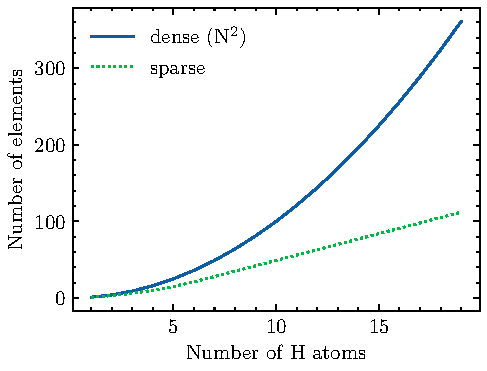
\includegraphics[scale=0.8]{Pics/overlap_nze}
\caption{}
\end{subfigure}
\begin{subfigure}{0.45\linewidth}
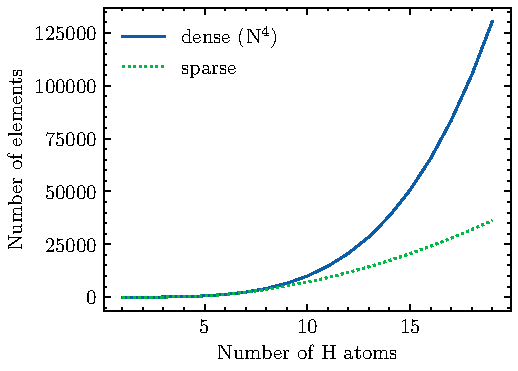
\includegraphics[scale=0.8]{Pics/eri_nze}
\caption{}
\end{subfigure}%
\caption[Sparsity of overlap and electron repulsion integrals]{(a) Number of significant entries (green line) in the overlap matrix for a hydrogen atom chain, with a threshold of 1e-10. The blue line shows the total number of elements for the dense matrix, which scale as $N^2$. (b) Number of significant entries (green line) in the electron repulsion integral tensor for a hydrogen atom chain, with a threshold of 1e-10. The blue line shows the total number of elements for the dense tensor, which scale as $N^4$.}
\label{fig:HCHAIN_ERINZE}
\end{figure}

\begin{figure}
\centering
\begin{subfigure}{0.45\linewidth}
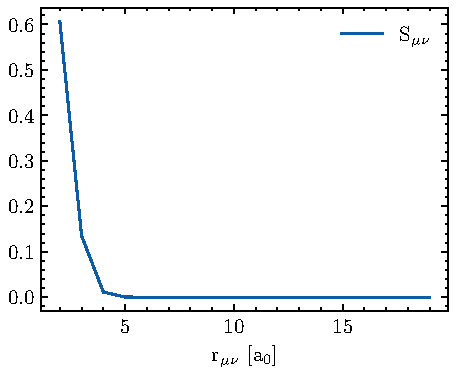
\includegraphics[scale=0.8]{Pics/overlap_decay}
\caption{}
\end{subfigure}
\begin{subfigure}{0.45\linewidth}
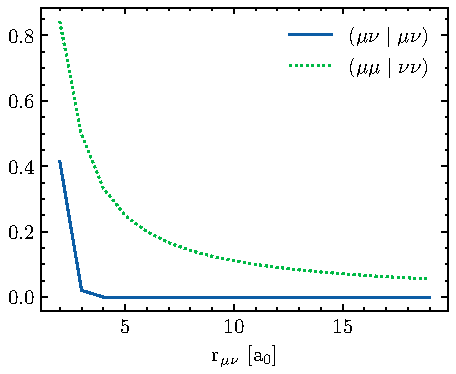
\includegraphics[scale=0.8]{Pics/eri_decay}
\caption{}
\end{subfigure}%
\caption[Decay of the overlap and electron repulsion integrals]{(a) Magnitude of the overlap integral between two Gaussian 1s orbitals as a function of distance $r$ (exponential decay). (b) Magnitude of the electron repulsion integral between two Gaussian 1s orbitals as a function of $r$. The short range interaction $\cn{\mu\nu}{\mu\nu}$ decays at a  much faster rate with $e^{-r^2}$, compared to the long range interaction $\cn{\mu\mu}{\nu\nu}$ with $1/R$.}
\label{fig:HCHAIN_DECAY}
\end{figure}

\subsubsection{Linear Scaling Overlap Integrals}

While the overlap integrals formerly scale with $\ccpx{2}$, the number of significant elements scales \emph{linearly}. First, consider the product of two 1s GTOs $\chi_{A}$ and $\chi_{B}$, centered at $\mathbf{A}$ and $\mathbf{B}$, with exponents $\alpha$ and $\beta$. The Gaussian product theorem (GPT) states that the result is itself a (scaled) Gaussian function
\begin{equation}
\chi(A,\alpha) \chi(B,\beta) = e^{-\alpha \left\lvert \mathbf{r} - \mathbf{A} \right\rvert^2} e^{-\beta \left\lvert \mathbf{r} - \mathbf{B} \right\rvert^2} = \kappa \chi(P,\alpha+\beta)  
\end{equation}
\noindent with the scaling factor $\kappa$ 
\begin{equation}
\kappa = e^{-\frac{\alpha\beta}{\alpha+\beta}\left\lvert \mathbf{A} - \mathbf{B} \right\rvert^2}
\end{equation}
\noindent and the center-of-charge coordinate $P$
\begin{equation}
\mathbf{P} = \frac{\alpha \mathbf{A} + \beta \mathbf{B}}{\alpha + \beta}
\end{equation}
\noindent Spatial integration yields the expression for the overlap between $\chi_A$ and $\chi_B$
\begin{equation}
S_{AB} = \int \kappa \chi_{P} dr = \kappa \left(\frac{\pi}{\alpha + \beta}\right)^{3/2}
\end{equation} 
\noindent The magnitude of the overlap integral is proportional to the scaling factor $\kappa$ which decays exponentially with the distance between GTO centers. In the case of the model system given above, where $\alpha = \beta$, the distance at which the integral falls below a certain threshold $\eps$ is given by 
\begin{equation}
d_s = \sqrt{\alpha^{-1} ln \left[ \left( \frac{\pi}{2\alpha}\right)^3 \eps^{-1/2} \right]}
\end{equation} 
\noindent Which in our case is equal to 6.9 $a_0$. Each hydrogen atom therefore only has significant overlap with a finite number $n_{max}$ of other centers. For atom chains with $n > n_{max}$, the number of non-zero elements in the overlap matrix will no longer scale as $n^2$, but \emph{linearly} with $n_{max}$. For more realistic, three-dimensional molecular systems, the crossover is less clearly defined due to the non-uniform distribution of atoms and different GTO exponents. Nonetheless, if a system grows sufficiently large, the overlap integrals still scale linearly. Similar arguments can be brought forth for the kinetic-energy integrals as well. 

\subsubsection{Quadratic Scaling Electron Repulsion Integrals} 

Using the Gaussian product theorem established above, we can express the two-electron repulsion integrals of four primitive 1s Gaussian functions $s(A,\alpha)$, $s(B,\beta)$, $s(C,\gamma)$ and $s(D,\delta)$ as
\begin{equation}
\begin{split}
g_{ABCD} &= \int s(A,\alpha) s(B,\beta) \frac{1}{\left\lvert \mathbf{r_1} - \mathbf{r_2} \right\rvert} s(C,\gamma) s(D,\delta) dr \\
&= \int \kappa s(P, \alpha+\beta) \frac{1}{\left\lvert \mathbf{r_1} - \mathbf{r_2} \right\rvert} \lambda s(Q, \gamma+\delta)
\end{split}
\end{equation}
\noindent where $s(P,p)$ and $s(Q,q)$ are Gaussian distributions with
\begin{equation}
\mathbf{P} = \frac{\alpha \mathbf{A} + \beta \mathbf{B}}{\alpha + \beta} ; \quad \mathbf{Q} = \frac{\gamma \mathbf{C} + \delta \mathbf{D}}{\gamma + \delta}
\end{equation}
\begin{equation}
\kappa = e^{-p\left\lvert \mathbf{A} - \mathbf{B} \right\rvert^2} ; \quad \lambda = e^{-q\left\lvert \mathbf{C} - \mathbf{D} \right\rvert^2}
\end{equation}
\begin{equation}
p = \frac{\alpha\beta}{\alpha+\beta}; \quad q = \frac{\gamma\delta}{\gamma+\delta}
\end{equation}

\noindent The Coulomb integrals can then be evaluated as 
\begin{equation}
g_{ABCD} = \sqrt{\frac{4 \eta}{\pi}} S_{AB} S_{CD} F_0\left(\eta \left\lvert \mathbf{P} - \mathbf{Q} \right\rvert^2 \right)
\end{equation}
\noindent with the Boys function $F_0$ and the reduced exponent $\eta$ given by
\begin{equation}
\eta = \frac{pq}{p+q}
\end{equation}

\noindent The Boys function is an important function appearing in many expressions for molecular integral evaluation. There are two expressions that bound the Boys function
\begin{equation}
\begin{split}
F_n(x) \leq \frac{1}{2n+1} \quad \textrm{for small } x \\
F_n(x) \leq \frac{(2n-1)!!}{2^{n+1}}\sqrt{\frac{\pi}{x^{2n+1}}} \quad \textrm{for large } x 
\end{split}
\end{equation}
\noindent Using the Boys function's upper bounds, we can derive an upper bound for the electron repulsion integrals of our model system
\begin{equation}
g_{ABCD} \leq min \left\lbrace \sqrt{\frac{4\eta}{\pi}} S_{AB} S_{CD}, \frac{S_{AB} S_{CD}}{\left\lvert \mathbf{P} - \mathbf{Q} \right\rvert} \right\rbrace
\end{equation}
\noindent The left-hand upper bound represents the short-range limit of the Boys function, and the right-hand one the long-range limit. In the short-range limit, i.e. for increasing distance $R_{AB}$ or $R_{CD}$, the magnitude of $g$ decreases \emph{exponentially}. As shown in the previous section, the non-zero elements of the overlap integrals $S_{AB}$ and $S_{CD}$ scale linearly with system size, and therefore the number of significant electron repulsion integrals scales with $N^2$ in total. 
It should be noted, that in the long-range limit with increasing distance $R_{PQ}$ between product densities, the number of elements in $g$ will eventually scale linearly. However, the \emph{algebraic} $1/R$ decay of the long-range interactions is so slow that it practically useless for the size of molecules that can be tackled with current technologies. In the case of the hydrogen atom chain, the integrals $\cn{\mu\mu}{\nu\nu}$ only fall below 1e-10 for $R_{PQ}$ greater than 10e+10 $a_0$. While the long-range decay is impractical for use in the case of the electron repulsion integrals, there are instances such as in atomic orbital MP2 (see Chapter $\ref{cha:LOCAL1}$) where \emph{bra} and \emph{ket} decay as $1/R^4$.
Knowing that the electron repulsion integrals are sparse is only the first step. One also has to develop a \emph{screening} method to avoid computing small integrals, by finding a general upper bound. It has been shown \cite{Roo1951} that $g$ is positive-definite, and fulfills the relationship
\begin{equation}
\sum_{abcd} c_{ab} g_{abcd} c_{cd} > 0
\end{equation}
\noindent where $c$ are one-electron orbital distributions. One can then apply the Schwarz inequality \cite{Hf1989} to obtain an upper bound expression for $g$
\begin{equation}
\cn{\mu\nu}{\sigma\lambda} \leq \cn{\mu\nu}{\mu\nu} \cn{\sigma\lambda}{\sigma\lambda} = Q_{\mu\nu} Q_{\sigma\lambda}
\end{equation}
\noindent The matrix $\mathbf{Q}$ contains the square root of the short-range diagonal entries of $g$, and is also known as the Schwarz matrix. $\mathbf{Q}$ can be evaluated quickly with $\ccpx{2}$ effort and individual integrals can be efficiently screened. It should be noted that Schwarz screening does not take into account the $1/R$ decay between product densities, which makes the method less useful in methods like AO-MP2.

\subsection{Element-Wise Sparsity of the Density Matrix}

The decaying behavior of the density matrix has been extensively studied in solids for atom-centered Bloch and Wannier functions \cite{Koh1959,Ism1999,Goe1994,Goe1998,Tar2002}. It was shown that for insulators, i.e. systems with large band-gaps, the contributions $P_{\mu\nu}$ decay exponentially with increasing distance $R_{\mu\nu}$, while for systems with small or no band gaps, such as metals, the elements decay algebraically. This is also known as Kohn's conjecture \cite{Koh1959}.  
The same observations have been made for non-periodic systems using atomic orbitals as basis. For molecules with a large HOMO-LUMO gap, e.g. alkanes, the number of non-zero elements in the atomic orbital density matrix scales linearly with increasing system size. On the other hand, molecules with strong electron delocalization, such as conjugated polyenes, have a small HOMO-LUMO gap, and the density matrix elements decay much slower. 
Consider again a chain of hydrogen atoms, equally spaced by $a_0$, each with one 1s Gaussian function, this time with $N_{atom}$ atoms. Figure \ref{fig:HCHAIN_DECAY}a shows the MO diagram for an increasing chain length. In the limit where $N_{atom} \rightarrow \infty$, the system takes on a band structure, similar to how they are encountered in a metal, with a smooth transition between occupied (valence) and virtual (conductance) band. In other words, the HOMO-LUMO gap becomes increasingly small. For a hydrogen chain, where each individual atom contributes one electron, the band is half filled, and the system is a conductor. If the Hydrogen atoms are replaced by Helium atoms, with two electrons per site, the band is fully filled and the system becomes an insulator.
The magnitude of the density matrix elements $P_{\mu\nu}$ is plotted in Figure \ref{fig:HCHAIN_DENSITY}b as a function of increasing distance between 1s functions. The elements decay much slower for the conducting hydrogen chain (algebraic decay), while a rapid exponential decay can be observed in the case of the insulating helium chain. An interesting thing to note is the oscillating values of the density matrix for the hydrogen chain. This phenomenon arises due to the hydrogen atoms pairing up into loosely bound $H_2$ molecules. 

\begin{figure}
\centering
\begin{subfigure}{0.45\linewidth}
\centering
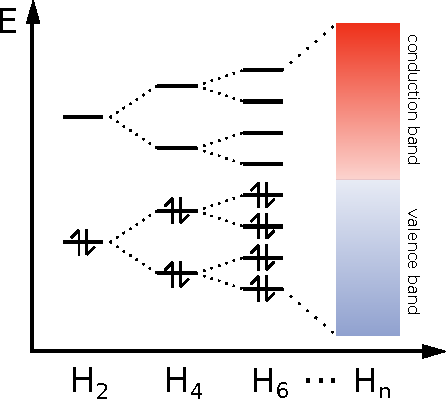
\includegraphics[scale=0.8]{Pics/MOchain}
\caption{}
\end{subfigure}
\begin{subfigure}{0.45\linewidth}
\centering
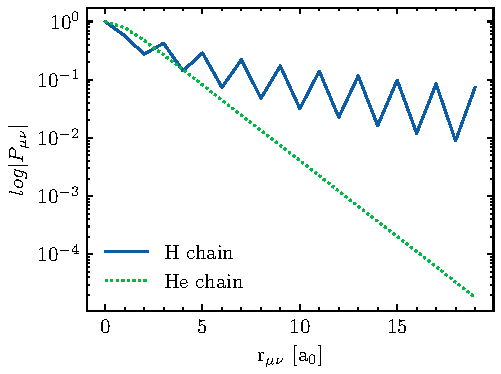
\includegraphics[scale=0.8]{Pics/density_decay}
\caption{}
\end{subfigure}
\caption[MO diagram and decay of density matrix elements in the infinite hydrogen chain]{(a) Molecular orbital diagram for a hydrogen with increasing chain length. (b) Logarithm of the absolute value of the density matrix element $P_{\mu\nu}$ as a function of increasing distance $R_{\mu\nu}$ for a Hydrogen and a Helium atom chain.}
\label{fig:HCHAIN_DENSITY}
\end{figure}


%This sparsity relationship between two AOs is also known as Kohn's conjecture (ref DLMP2).
% exponential decay:
% Koh1959 https://journals.aps.org/pr/abstract/10.1103/PhysRev.115.809
% Ism1999 https://journals.aps.org/prl/abstract/10.1103/PhysRevLett.82.2127
% Goe1994 https://journals.aps.org/prl/pdf/10.1103/PhysRevLett.73.122
% Goe1998 https://journals.aps.org/prb/pdf/10.1103/PhysRevB.58.3501

% algebraic decay
% Tar2002 https://journals.aps.org/prb/abstract/10.1103/PhysRevB.66.233101

\subsection{Diagrammatic Notation}

Hollmann et al. \cite{Hol2017} introduced a simple graphical representation to show contributing factors to the sparsity of a given matrix, tensor or tensor contraction. Each tensor index is represented as a vertex. Non-connected vertices each contribute $\mathcal{O}(N)$ elements to the overall expression. A sparsity relationship between two indices is represented as an \emph{edge} connecting two vertices. In that case, the number of \emph{pairs} scales as $\mathcal{O}(N)$. Consider the two electron integral tensor $\cn{\mu\nu}{\sigma\lambda}$. From the previous section, we know that the index pairs $\mu,\nu$ and $\lambda,\sigma$ are related by overlap. The diagrammatic representation takes the form:
\begin{center}
\begin{tikzpicture}

\snode{MU}{0,0}{\mu};
\snode{NU}{1,0}{\nu};
\snode{SIG}{2,0}{\sigma};
\snode{LAM}{3,0}{\lambda};

\draw[<->] (MU) -- (NU) node [midway, above] () {S};
\draw[<->] (SIG) -- (LAM) node [midway, above] () {S};

\end{tikzpicture}
\end{center}
\noindent There are two pairs of connected vertices, which indicates that the integrals can be evaluated with $\ccpx{2}$ effort, which is in agreement with the findings above. The $S$ denotes the overlap relationship between vertices.
For another example, consider the Hartree-Fock expression for the exchange matrix
\begin{equation}
K_{\mu\nu} = \cn{\mu\sigma}{\nu\lambda} P_{\lambda\sigma}
\end{equation}
\noindent Diagrammatically, the expression for $\mathbf{K}$ can be represented as
\begin{center}
\begin{tikzpicture}

\snode{MU}{0,0}{\mu};
\snode{NU}{3,0}{\nu};
\snode{SIG}{1,0}{\sigma};
\snode{LAM}{2,0}{\lambda};

\draw[<->] (MU) -- (SIG) node [midway, above] () {S};
\draw[<->] (SIG) -- (LAM) node [midway, above] () {P};
\draw[<->] (LAM) -- (NU) node [midway, above] () {S};

\end{tikzpicture}
\end{center}
\noindent The connection between $\sigma$ and $\lambda$ is also known as a "P-junction" \cite{Nee2009}, which represents the sparsity relationship arising due to the exponential decay of density matrix elements. The sparsity graph is fully connected, which suggests that $\mathbf{K}$ can be evaluated with $\mathcal{O}(N)$ effort. This is indeed the case, as shown by the ONX or LinK method. For linear scaling to emerge, indices of an expression therefore need to be fully linked. This simple but important fact is also known the linked index rule (LIR). Diagrams also show which factors can influence the performance of the scaling, such as diffuseness of the atomic orbitals (slower S decay) or size of of the HOMO-LUMO gap (slower P decay). One can therefore conclude that the expression for $\mathbf{K}$ as given above, is less suitable for large basis sets and conducting systems.

\subsection{Rank Sparsity}

A positive semi-definite matrix $\mathbf{A}$ has the property that it can be decomposed as a product 
\begin{equation}
\mathbf{A} = \mathbf{B} \mathbf{B}^T
\end{equation}
\noindent where $\mathbf{A}$ has dimensions $N$ by $N$, and $\mathbf{B}$ has dimensions $N$ by $rank(A)$. The rank represents the number of linearly independent column vectors in a matrix, and for $rank(A) < N$, the matrix is said to  be rank-deficient. The decomposition matrix $\mathbf{B}$ therefore is more compact and needs less storage space than $\mathbf{A}$. There are different ways to compute $\mathbf{B}$, such as Cholesky decomposition or QR decomposition.
The tensor $\cn{\mu\nu}{\sigma\lambda}$ can be represented as a $N_{AO}^2$
by $N_{AO}^2$ matrix with combined row indices $I = \mu + N_{AO}*\nu$ and column indices $J = \sigma + N_{AO}*\lambda$. Because the tensor has been shown to be positive semi-definite, there exists a decomposition, such that
\begin{equation}
\cn{\mu\nu}{\sigma\lambda} = A_{(\mu\nu)(\sigma\lambda)} = B_{(\mu\nu)X} B_{(\sigma\lambda)X}
\end{equation}
\noindent The rank of $\mathbf{A}$ is in general much smaller than the combined index range $N_{AO}^2$, and scales linearly rather than quadratically with the number of basis functions. The decomposition tensor $\mathbf{B}$ is therefore 3-dimensional, rather than 4-dimensional, which reduces the storage needed by an order of magnitude from $\ccpx{4}$ to $\ccpx{3}$, ignoring sparsity. In the limit of large molecules, the NZEs of $\mathbf{B}$ also scale with $\ccpx{2}$. Rather than for the molecular integrals in the AO basis, decomposition techniques are more useful for reducing the storage size of molecular integrals in the canonical MO basis
\begin{equation}
\cn{ia}{jb} = C_{\mu i} C_{\sigma a} B_{\mu \sigma X} B_{X \nu \lambda} C_{\nu j} C_{\lambda b} = B_{iaX} B_{Xjb}
\end{equation} 
\noindent The AO-MO transformation step is drastically sped up, but remains a $\ccpx{4}$ effort. Rank sparsity has therefore little impact on the overall scaling, but rather reduces the scaling \emph{prefactor}. Over the years, different methods have been proposed to compute $\mathbf{C}$, such as density fitting, Cholesky decomposition, pseudo-spectral methods, or tensor hypercontraction.
Density matrices at different levels of theory (Hartree Fock, MP2, CC ...) also exhibit rank sparsity. Decomposition of such matrices play an important role in local molecular orbital schemes and low scaling electronic structure methods, as will be shown in later sections.

% pos def Roo1951 C. C. J. Roothaan, Rev. Mod. Phys., 23, 69 (1951).

% Schwarz inequality Has1989 https://onlinelibrary.wiley.com/doi/abs/10.1002/jcc.540100111

% Good explanation for "linked indices rule" https://aip.scitation.org/doi/pdf/10.1063/1.4926879

% Nee2009 https://reader.elsevier.com/reader/sd/pii/S0301010408005089?token=A38BA6311BBE21191E796ADD75EF1602618F281416BBB8E8C22D61B0C75DF4C02EF402A33375738162D7AA02AFAB8685&originRegion=eu-west-1&originCreation=20210707062425

\FloatBarrier

\section{Density Fitting}

The method of choice in this thesis for the decomposition of two-electron molecular integrals is \emph{density fitting} (DF), also known as \emph{resolution of the identity} (RI). Techniques such as Cholesky decomposition \cite{Koc2003,Roe2008} or tensor hypercontraction (THC) \cite{Hoh2012,Par2012,Hoh2012a} are not discussed here. 

\subsection{Basics of Density Fitting}

The two-electron integrals can be expressed in terms of the charge product densities $\rho_{\mu\nu} = \chi_{\mu} \chi_{\nu}$ as
\begin{equation}
\cn{\mu\nu}{\sigma\lambda} = \int \int \frac{\rho_{\mu\nu}(\mathbf{r_1}) \rho_{\sigma\lambda}(\mathbf{r_2}) }{\left\lvert \mathbf{r_1} - \mathbf{r_2} \right\rvert} d\mathbf{r_1} d\mathbf{r_2}
\end{equation}
The charge densities $\rho$ can be approximated by fitting them to a set of atom-centered auxiliary functions $\chi_P$
\begin{equation}
\rho_{\mu\nu}(\mathbf{r}) = C_{P\mu\nu} \chi_{P}(\mathbf{r}) + \Delta \rho_{\mu\nu}
\end{equation}
\noindent Or in the chemist's notation:
\begin{equation}
\cket{\mu\nu} = C_{P\mu\nu} \cket{P} + \cket{\eps_{\mu\nu}} = \cket{\swtilde{\mu\nu}} + \cket{\eps_{\mu\nu}}
\label{eq:DFAPPROX}
\end{equation}
\noindent where $C_{P\mu\nu}$ are the fitting coefficients, and $\Delta \rho_{\mu\nu}$ or $\cket{\eps_{\mu\nu}}$ is the error introduced by the fitting procedure. Equation \ref{eq:DFAPPROX} is known as the density fitting approximation \cite{Whi1973,Bae1973,Vah1993,Sky2000}. The two-electron integrals then take the form
\begin{equation}
\begin{split}
\cn{\mu\nu}{\sigma\lambda} &= (\swtilde{\mu\nu}|\swtilde{\sigma\lambda}) +  \underbrace{(\swtilde{\mu\nu}|\eps_{\sigma\lambda}) + (\eps_{\mu\nu}|\swtilde{\sigma\lambda})}_\textrm{first order} + \underbrace{\cn{\eps_{\mu\nu}}{\eps_{\sigma\lambda}}}_\textrm{second order} \\
&= (\swtilde{\mu\nu}|\swtilde{\sigma\lambda}) + \eps_J^{(1)} + \eps_J^{(2)} 
\end{split}
\label{eq:DFERROR}
\end{equation}
\noindent Here, $\eps_J^{(1)}$ and $\eps_J^{(2)}$ represent the first order (linear) and second order (quadratic) error. The fitting coefficients are then generally found by minimizing $\eps_J^{(2)}$. Substituting $\scbra{\eps_{\mu\nu}} = \scbra{\mu\nu - \swtilde{\mu\nu}}$ gives
\begin{equation}
\frac{\partial}{\partial C^P_{\mu\nu}} \scn{\mu\nu - \swtilde{\mu\nu}}{\sigma\lambda - \swtilde{\sigma\lambda}} = 0
\end{equation}
\noindent which then yields a set of linear equations
\begin{equation}
\scn{\mu\nu}{P} - \sum_Q C^Q_{\mu\nu} \scn{Q}{P} = 0 
\label{eq:DFLLS}
\end{equation}
\noindent Finding the fitting coefficients by minimizing $\eps_J^{(2)}$ has the important feature that $\eps_J^{(1)} = 0$, which can be shown by substituting Equation \ref{eq:DFLLS} back into Equation \ref{eq:DFERROR}. The total electron integral error is therefore \emph{quadratic} in the fitting error. Fitting procedures where the coefficients $C^P_{\mu\nu}$ satisfy Equation \ref{eq:DFLLS} are termed $\emph{robust}$ \cite{Dun2000}. Any restrictions posed on $C^P_{\mu\nu}$ makes $\eps_{1}$ different from zero and the error scales linearly. 
Equation \ref{eq:DFLLS} requires the evaluation of the three-center-two-electron (3c2e) and two-center-two-electron (2c2e) integrals in the auxiliary basis set $\{P\}$
\begin{equation}
\cn{\mu\nu}{P} = \int \int \chi_{\mu}(\mathbf{r_1}) \chi_{\mu}(\mathbf{r_1}) \frac{1}{\left\vert \mathbf{r_1} - \mathbf{r_2} \right\rvert} \chi_{P}(\mathbf{r_2}) d\mathbf{r_1} d\mathbf{r_2} 
\end{equation}
\begin{equation}
\cn{P}{Q} = \int \int \chi_{P}(\mathbf{r_1}) \frac{1}{\left\lvert \mathbf{r_1} - \mathbf{r_2} \right\rvert} \chi_{Q}(\mathbf{r_2}) d\mathbf{r_1} d\mathbf{r_2} 
\end{equation}
\noindent The fitting coefficients are generally computed by inverting $\cn{P}{Q}$, which leads to the following approximation for the four-center-two-electron integrals (4c2e)
\begin{equation}
\cn{\mu\nu}{\sigma\lambda} \approx \cn{\mu\nu}{P} \cn{P}{Q}^{-1} \cn{Q}{\sigma\lambda}
\end{equation}
\noindent Matrix inversion is a $\ccpx{3}$ computational effort. 
%For more details on precision and best practices involving matrix inversion, see Annex \ref{app:MATINV}.
% Introduced independently by
% (Coulomb) Whi73 https://aip.scitation.org/doi/10.1063/1.1679012
% (Overlap) Bae1973 https://doi.org/10.1016/S0301-0104(99)00271-2 2, 41 (1973).
% Dunlap improved Baerends by using coulomb instead of overlap
% Dun1979 https://aip.scitation.org/doi/pdf/10.1063/1.438728
% Dun1979a https://doi.org/10.1063/1.438313 71, 4993 (1979).
% Begriff "Robust" erstmals hier
% Dun2000 https://www.sciencedirect.com/science/article/pii/S0166128099004339?via%3Dihub

\subsection{Scaling of the 3c2e Integrals}

Using the diagrammatic representation introduced earlier, the 3c2e integral tensor reduces to
\begin{center}
\begin{tikzpicture}
\snode{MU}{0,0}{\mu};
\snode{NU}{1,0}{\nu};
\snode{X}{2,0}{P};
\draw[<->] (MU) -- (NU) node [midway, above] () {S};
\end{tikzpicture}
\end{center}
The number of non-zero elements therefore scales as $\ccpx{2}$, just like for the 4c2e integrals. Similarly, the Schwarz inequality can be used to screen out small integrals
\begin{equation}
\left\lvert \cn{\mu\nu}{P} \right\rvert \leq \left\lvert \cn{\mu\nu}{\mu\nu} \right\rvert^{1/2} \left\lvert \cn{P}{P} \right\rvert^{1/2}
\end{equation}
\noindent As mentioned above, Schwarz screening does not take into account increasing bra-ket distance. The long-range decay is too slow to be of any advantage in the case of the 4c2e integrals. However, it was found \cite{Hol2015} that for an auxiliary density $\chi_P(\mathbf{r}$ with angular momentum $l_P$, the 3c2e integrals actually decay as $1/R^{-1 - l_P}$ with increasing bra-ket distance, establishing a weak but not insignificant sparsity relationship between $\cbra{\mu\nu}$ and $\cket{P}$ 
\begin{center}
\begin{tikzpicture}
\snode{MU}{0,0}{\mu};
\snode{NU}{1,0}{\nu};
\snode{MUNU}{0.5,0}{};
\snode{X}{2,0}{P};
\draw[<->] (MU) -- (NU) node [midway, above] () {S};
\draw[dotted] (MUNU.south) |- (1.25, -0.5) node [below]{$1/R^{-1-l_P}$} -| (X.south);
\end{tikzpicture}
\end{center}
\noindent In principle, the 3c2e integrals can be evaluated with linear effort. Hollmann et al. \cite{Hol2015} have introduced a tight upper bound, known as the SVQl estimator, to exploit this faster decay. Due to the dependence on $l_P$, the screening is most effective with larger basis sets with high angular momentum functions.

The fitting coefficients evaluated as $C^P_{\mu\nu} = \cn{\mu\nu}{Q} \cn{Q}{P}^{-1}$ formerly scale with $\ccpx{3}$
\begin{center}
\begin{tikzpicture}
\snode{MU}{0,0}{\mu};
\snode{NU}{1,0}{\nu};
\snode{Q}{2,0}{Q};
\snode{P}{3,0}{P};
\draw[<->] (MU) -- (NU) node [midway, above] () {S};
\end{tikzpicture}
\end{center}
\noindent due to the inverse of $\cn{P}{Q}$ not being sparse. 

\subsection{Local Density Fitting: Principles} 
The long-range behavior introduced by Equation \ref{eq:DFLLS} is often deemed "unphysical" \cite{Tew2018}. \emph{Local density fitting} (LDF) methods circumvent this problem by forcing a more rapid decay of long-range contributions, either (a) by using a different metric in the fitting procedure or (b) by constructing domains $[\mu\nu]$ that exclude distant fitting functions $P$ a priori. In both cases, Equation \ref{eq:DFLLS} no longer holds and the error in the electron integrals increases linearly with the fitting error. Therefore, the density fitting procedure is no longer robust. Fortunately, LDF methods can use a different expression for the electron integrals which includes the first order terms to remove the linear error
\begin{equation}
\cn{\mu\nu}{\sigma\lambda} \approx (\widetilde{\mu\nu}|\sigma\lambda) + (\mu\nu|\widetilde{\sigma\lambda}) - (\widetilde{\mu\nu}|\widetilde{\sigma\lambda})
\label{eq:DUNLAP}
\end{equation}
\noindent which is known as Dunlap's robust density fitting formula \cite{Dun2000}. It greatly increases accuracy for LDF. 
 
\subsection{LDF (I): Short-Range Metrics}
The first type of LDF methods replaces the fitting procedure in the Coulomb metric in Equation \ref{eq:DFLLS} by a more general expression
\begin{equation}
B_{\mu\nu}^{P} - C_{\mu\nu}^{Q} M_{QP} = 0
\end{equation}  
\noindent where $B_{\mu\nu}^{P}$ and $M_{PQ}$ are the 3c2e and 2c2e integrals given by
\begin{equation}
B_{\mu\nu}^P = \int\int \bfun{\mu}{1}\bfun{\nu}{1} g(\mbf{r_1},\mbf{r_2}) \bfun{P}{2} d\mbf{r_1} d\mbf{r_2}
\end{equation}
\begin{equation}
M_{PQ} = \int\int \bfun{P}{1} g(\mbf{r_1},\mbf{r_2}) \bfun{Q}{2} d\mbf{r_1} d\mbf{r_2}
\end{equation}
\noindent with $g$ being the operator for the local metric. A list of known local metrics is given in Table \ref{tab:DFMETRICS}. Earliest forms of density fitting actually first used an overlap metric to directly minimize the norm of the residual $R_{\mu\nu} = \cbra{\mu\nu} - \cbra{\widetilde{\mu\nu}}$ by the linear least squares methods \cite{Bae1973}, and the fitting coefficients are computed as
\begin{equation}
C^P_{\mu\nu} = S_{PQ}^{-1} (\mu\nu Q)
\label{eq:OVLPMET}
\end{equation}
\noindent where $S_{PQ}$ is the overlap matrix of the auxiliary basis, and $(\mu\nu Q)$ are the 3-center-\textbf{1-electron} overlap integrals. While the overlap metric has the most rapid decay and the quantities in Equation \ref{eq:OVLPMET} can be evaluated in $\mathcal{O}(N)$ time, it has the worst accuracy of all metrics. One solution to this problem is to introduce a metric which is intermediate between overlap and coulomb fitting. Examples include the Yukawa, Coulomb- and Gaussian-attenuated metrics. These intermediate metrics introduce a damping factor $\omega$ to control the sparsity and accuracy of the density fit. In the limit where $\omega \rightarrow 0$, and $\omega \rightarrow \infty$, one recovers the coulomb and overlap metric, respectively. Figure \ref{fig:DFMETRICS} shows the decay behavior of the Coulomb-attenuated metric, for $\omega$ = 0.01, 0.1 and 1.0, compared to the overlap and the Coulomb metric. 

\begin{table}
\centering
\begin{tabular}{cc}
\hline
Metric & $g(r_{12})$ \\ \hline
\multirow{2}{*}{Overlap \cite{Bae1973}} & \multirow{2}{*}{1} \\ & \\
\multirow{3}{*}{Coulomb-Attenuated \cite{Jun2005}} & \multirow{3}{*}{$\dfrac{\mathrm{erfc}(\omega r_{12})}{r_{12}}$} \\ & \\ & \\
\multirow{3}{*}{Yukawa \cite{Gil2005}} & \multirow{3}{*}{$\dfrac{e^{-\omega r_{12}}}{r_{12}}$} \\ & \\ & \\
\multirow{3}{*}{Gaussian-Damped \cite{Rei2008}} & \multirow{3}{*}{$\dfrac{e^{-\omega r_{12}^2}}{r_{12}}$} \\ & \\ & \\ \hline
\end{tabular}
\caption{Expressions for the operator $g$ in different local metrics.}
\label{tab:DFMETRICS}
\end{table}

\begin{figure}
\centering
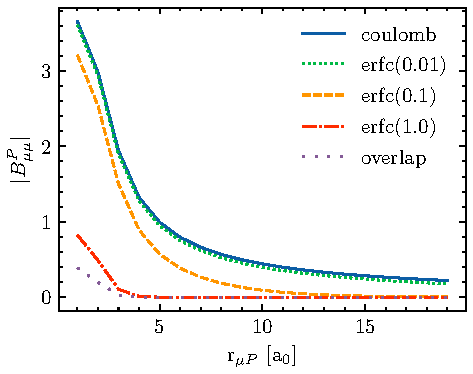
\includegraphics[scale=1.0]{Pics/ldf.pdf}
\caption{Absolute value of the 3c2e integral $B_{\mu\mu P}$ between two 1s GTOs $\mu$ and $P$ with $\alpha$ = 1.0 using different metrics.}
\label{fig:DFMETRICS}
\end{figure}

% A:
% Bae1973 https://www.sciencedirect.com/science/article/pii/030101047380059X?via%3Dihub
% Vah1993 https://www.sciencedirect.com/science/article/pii/0009261493891517?via%3Dihub
% Sky2000 https://www.sciencedirect.com/science/article/pii/S0166128099004340?via%3Dihub
% B: Jun2005 https://www.pnas.org/content/102/19/6692 
% C: Gil2005 https://aip.scitation.org/doi/10.1063/1.2000867 
% D: Rei2008 https://aip.scitation.org/doi/10.1063/1.2956507

% Hol2015 D.S. Hollman, H.F. Schaefer, and E.F. Valeev, J. Chem.Phys.142(2015)

\subsection{LDF (II): Local Domains}

The second method to force locality in density fitting consists in constructing local domains for each atom, pair of atoms or local molecular orbital, and excluding any auxiliary functions that lie outside, which can drastically reduce the dimension of the fitting procedure. 

\subsubsection{Atomic Resolution of the Identity}

The simplest example of a domain is one that includes a single atom. The atomic resolution of the identity (ARI) \cite{Sod2008} uses a fitting procedure where the sum over auxiliary function $Q$ only includes those which are centered on the same atom $A$ as the atomic orbital $\mu$
\begin{equation}
\cket{\widetilde{\mu\nu}} = \sum_{Q \cup A_{\mu}} \cn{P}{Q}_{A_{\mu}}^{-1} \cn{\mu\nu}{Q}
\end{equation}
\noindent Each atom $X$ has its own metric matrix inverse $\cn{P}{Q}_X^{-1}$ which takes the form 
\begin{equation}
\cn{P}{Q}_X^{-1} = B_X \left( \cn{P}{Q}_D + B_X \cn{P}{Q}_{OD}B_X\right)^{-1}B_X
\end{equation}
\noindent where $\cn{P}{Q}_D$ and $\cn{P}{Q}_{OD}$ are the diagonal and off-diagonal part of $\cn{P}{Q}$ respectively. $B_X$ is a so-called \emph{bump matrix} which imposes a fast, but smooth decay between functions $P$ and $Q$ in order to avoid using all functions $P$ for the fitting. For further details, the reader is referred to the original publication. The bump matrix uses multiple distance-dependent criteria which make the ARI less of a black-box method.

% Sod2008 https://aip.scitation.org/doi/pdf/10.1063/1.2828533

\subsubsection{Pair-Atomic Resolution of the Identity}

A more popular and simple variant of atomic density fitting is the pair-atomic resolution of the identity (PARI) method \cite{Mer2013}. As the name implies, the domains include atom \emph{pairs} rather than a single atom. Again expressing it in terms of the fitting procedure
\begin{equation}
\cn{P}{\mu\nu} = \sum_{Q \in A \cup B} \cn{P}{Q} C^Q_{\mu\nu} \quad \forall P \in A \cup B
\end{equation}
\noindent The number of linear equations is equal to the number of non-zero pairs $\mu\nu$, which scales linearly. However, the PARI approach enforces heavy constraints on the fitting coefficients, which leads to large integral errors. Merlot et al. proposed to increase the atomic pair domain with any atoms which lie between A and B. Alternatively, larger and more diffuse basis sets can be used. In both cases, performance is sacrificed for increased accuracy. The absence of any distance dependent parameters or thresholds still make it an attractive method both for Hartree Fock and Post-Hartree Fock methods \cite{Man2015,For2020}.

% Mer2013 https://onlinelibrary.wiley.com/doi/full/10.1002/jcc.23284

\subsubsection{LDF using Local Molecular Orbitals}

Finally, domains can also be formed using local molecular orbitals instead of AOs. LMOs are larger than AOs, but are still generally centered on only a few atoms. The exact atomic sites can be determined for example by using a Mulliken population analysis. Consider the density fitting procedure as proposed by Polly et al. for their LDF-Hartree Fock method \cite{Pol2004}
\begin{equation}
\cn{\mu i}{P} = \sum_{Q \in [i]_{fit}} \cn{P}{Q} C^Q_{\mu i}
\end{equation}
The fitting coefficients are determined individually for each AO-LMO pair $\cket{\mu i}$, and include only those auxiliary functions centered on atoms in the fitting domain $[i]_{fit}$ for which the Mulliken charges are above a given threshold. Although the fitting coefficients need to be recomputed for each update of the MO coefficients, the number of $\cket{\mu i}$ pairs scales linearly with system size. This type of local density fitting and variations thereof are predominantly used in pair-orbital specific local correlation methods, and will be explained in more detail further below. 

% Pol2004 Fast Hartree–Fock theory using local densityfitting approximations

\subsection{LDF (III): Quasi-Robust Density Fitting}

Local density fitting imposes constraints on the fitting procedure, and the integral error consequently scales linearly with the fitting error. Using Dunlap's robust formula is deemed necessary in most cases to achieve acceptable accuracy, but reintroduces the slowly decaying 3c2e integrals. Furthermore, replacing the 4c2e integrals by Equation \ref{eq:DUNLAP} greatly increases the complexity of expressions in electronic structure theory, which is still manageable for ground state methods, but quickly becomes cumbersome for excited states.

Quasi-robust density fitting (QRDF) \cite{Tew2018} aims to combine the exponential decay behavior of LDF with an accuracy comparable to standard density fitting, without the use of Dunlap's formula. Again, consider the fitting procedure 
\begin{equation}
\sum_Q \cn{P}{Q} C^Q_{\mu\nu} = \cn{P}{\mu\nu}
\end{equation}
\noindent The sets of auxiliary functions $\{P\}$ and $\{Q\}$ have different roles. The functions $Q$ fit the charge density $\cket{\mu\nu}$, while the $P$ functions act as \emph{test functions} where the electron integrals should be accurate, i.e. where $\cn{X}{\widetilde{\mu\nu}} \approx \cn{X}{\mu\nu}$. For two functions $\mu$ and $\nu$ not located on the same atom, their charge density $\cket{\mu\nu}$ lies in the vacuum between them, and the atom-centered auxiliary functions may be ill-suited to fit $\cket{\mu\nu}$. For this reason, the fitting procedure draws from all fitting functions $\{P\}$ spanning the whole molecule to cancel out the linear error, which in consequence introduces long-range contributions in $C_{\mu\nu}^P$ in the coulomb metric, even if $\cket{P}$ is not close to $\cket{\mu\nu}$. 
The basic idea of QRDF is to only chose fitting functions $\{P\}$ close to $\cket{\mu\nu}$ via overlap criteria, but still perform the fitting procedure in the coulomb metric.

\subsubsection{The QRDF Fitting Procedure}

For a set of given $\mu,\nu$, select a set of \emph{fitting function} $\{P_{\mu\nu}\} \in \{P\}$ close to $\cket{\mu\nu}$ according to the criteria
\begin{equation}
\left\lvert \sum_R S_{PR}^{-1} (R\mu\nu) \right\rvert > T 
\label{eq:QRDF_FIT}
\end{equation} 
\noindent where $S$ is the auxiliary overlap matrix, and $(R\mu\nu)$ are the 3-center-1-electron overlap integrals. Next, choose a set of test functions $\{Q_{\mu\nu}\} \in \{P\}$ using
\begin{equation}
f(Q_{\mu\nu},P_{\mu\nu}) < R
\label{eq:QRDF_TEST}
\end{equation}
\noindent with
\begin{equation}
f(A,B) = \frac{\alpha \beta}{\alpha + \beta} \left\lvert \mathbf{A} - \mathbf{B} \right\rvert^2
\end{equation}
\noindent where for two auxiliary functions $A$ and $B$, the values $\alpha$, $\beta$ are their smallest primitive exponents and $\mathbf{A}$, $\mathbf{B}$ are their respective positions. The fitting coefficients are then determined via
\begin{equation}
\sum_P \cn{Q_{\mu\nu}}{P_{\mu\nu}} C^P_{\mu\nu} = \cn{Q_{\mu\nu}}{\mu\nu}
\label{eq:QRDFLLS}
\end{equation}
\noindent where the fitting coefficients are accurate within the set of test functions $\{Q_{\mu\nu}\}$. The linear equations in Equation \ref{eq:QRDFLLS} can be solved via QR decomposition or singular value decomposition (SVD) of the rectangular matrix $\cn{Q_{\mu\nu}}{P_{\mu\nu}}$.
The QRDF scheme depends on two parameters, $T$ and $R$. In the limit where $T \rightarrow 0$ and $R \rightarrow \infty$, the standard fitting procedure in the Coulomb metric is recovered. 

The fitting functions $\{P_{\mu\nu}\}$ are selected via overlap criteria and therefore scale linearly with the number of pairs $\cket{\mu\nu}$, and consequently the same holds true for the number of test functions $\{Q_{\mu\nu}\}$ close to $\{P_{\mu\nu}\}$ chosen by Equation \ref{eq:QRDF_FIT}. In the limit of large molecules, the size of the rectangular matrix in Equation \ref{eq:QRDF_TEST} becomes constant and the fitting procedure can be evaluated with $\mathcal{O}(N)$ effort. However, a QR decomposition needs to be computed for each set of $\cket{\mu\nu}$, leading to relatively high prefactor which makes the method not competitive for dense 3D structures like water clusters, as will be discussed in the results section.
The QRDF method has been shown to deliver accuracies comparable to standard density fitting, without the use of Dunlap's formula, making it a very attractive alternative to other LDF schemes, especially if one wishes to reduce the complexity of expressions involving LDF.

\subsection{Auxiliary Basis Sets}

The density fitting approximation does not make any assumptions about the size or shape of the auxiliary basis set used. In principle, the fit is exact for the basis set containing all $N_{AO}^2$ Gaussian products $\chi_P = \chi_{\mu} \chi_{\nu}$. In practice, the product space is over-complete and can be represented by much smaller basis sets. Accurate results can be obtained for auxiliary basis sets which are about four times larger than the principal basis set they are used with. 

Auxiliary basis sets generally need more higher angular momentum functions than standard basis sets. Consider an isolated, unperturbed atom, with electrons occupying atomic orbitals with highest angular momentum $l_{occ}$. A minimal basis set for this atom contains functions of angular momenta 0 to $l_{occ}$. However, a minimal auxiliary basis set for fitting the product space $\chi_{\mu}^{(0...l_{occ})} \chi_{\nu}^{(0...l_{occ})}$ needs functions with maximum angular momentum $2l_{occ}$. For example, 2nd row elements ($l_{occ}$ = 1) need an auxiliary basis set containing d-functions, and first row transition metals ($l_{occ}$ = 2) even need g-functions. Similarly to standard basis sets, to describe atoms in molecules where the orbitals are subject to polarization effects, even higher angular momentum functions are needed to fit polarization functions. In practice, a principal basis set with maximum angular momentum $l_{bas}$ is paired with an auxiliary basis set with highest angular momentum $l_{bas} + l_{occ}$. 

Auxiliary basis sets have the drawback of being method-specific. There are two categories: auxiliary basis sets for density fitted Hartree-Fock (DF-HF) and for density fitted correlated methods (e.g. DF-MP2, DF-CCSD, DF-ADC(2)). Auxiliary basis sets for DF-HF not only need to reproduce Hartree Fock energies, but also need to minimize negative impact on post-Hartree methods. An ill-suited auxiliary basis set leads to a deterioration of the virtual orbital space, and hence an increased error for correlated methods. 

Optimization procedures often try to minimize the energy differences between the standard method and its density fitting approximation in a series of atomic calculations. For example, the jkfit family of basis sets (cc-pVXZ-JKFIT \cite{Wei2002}, def-XVP-JKFIT \cite{Wei2008}) minimize the error
\begin{equation}
\Delta E_{HF} = E_{HF} - E_{DF-HF}
\end{equation}
The RI basis set family (cc-pVXZ-RIFIT \cite{Wei1998}, def2-XVP-RIFIT \cite{Ber1998}) minimizes the same energy difference but for MP2 or Coupled Cluster. 

Another disadvantage of auxiliary basis sets is that the accuracy of the fitting procedure cannot be easily controlled as a function of its composition (number of functions, angular momenta...), but rather extensive benchmarks are needed for each basis set that is introduced. An alternative approach was proposed by Aquilante et al. \cite{Aqu2007} where the fitting basis sets are generated automatically by Cholesky decomposition of the atomic 2-electron integrals
\begin{equation}
\cn{\mu\nu}{\sigma\lambda} = L^X_{\mu\nu} L^X_{\sigma\lambda}
\end{equation}
\noindent The Cholesky vectors $\mathbf{L}_{\mu\nu}$ indicate which product densities should be taken to construct the auxiliary basis. This type of atomic Cholesky decomposition (aCD) basis sets has the advantage that the accuracy can be rigorously controlled by the decomposition threshold $\theta$. To remove linear dependencies in the aCD basis set, another Cholesky decomposition can be performed to yield the atomic compact Cholesky decomposition (acCD) auxiliary basis set \cite{Aqu2009}.

% Dunning JKFIT (1): Wei2002 https://pubs.rsc.org/en/content/articlepdf/2002/cp/b204199p
% Karlsruhe JKFIT (2): Wei2007 https://onlinelibrary.wiley.com/doi/full/10.1002/jcc.20702
% MP2 Karlsruhe Wei1998 https://www.sciencedirect.com/science/article/pii/S0009261498008628
% Dunning (MP2) Ber1998 https://aip.scitation.org/doi/pdf/10.1063/1.476732
% Aqu2007 https://aip.scitation.org/doi/10.1063/1.2777146
% Aqu2009 https://aip.scitation.org/doi/10.1063/1.3116784

\section{Multipole Expansion of the Electron Integrals}

The slow $1/R$ decay between the product densities $\Omega_{\mu\nu}$ and $\Omega_{\lambda\sigma}$ in the coulomb integrals is a major obstacle for achieving linear scaling in cases where no other sparsity relationship can be established between indices belonging to separate charge densities, e.g. in the evaluation of the coulomb matrix $\mathbf{J}$ versus the exchange matrix $\mathbf{K}$. Luckily, there are approximate methods for integral evaluation that can be computed with $\mathcal{O}(N)$ effort, known as \emph{multipole methods}.

\subsection{Classical and Non-Classical Electron Integrals}

First, consider the concept of classical and non-classical interactions. Two-electron integrals are said to be \emph{non-classical} if the two charge densities $\Omega_{\mu\nu}$ and $\Omega_{\sigma\lambda}$ overlap, and \emph{classical} if the charge densities are well separated. In the latter case, the electron integrals represent classical interactions between disjoint point charges, and can be approximated using multipole methods, whereas the non-classical contributions must be evaluated using the more expensive standard integral codes such as McMurchie-Davidson or Obara-Saika. 

Two Gaussian distributions $\Omega_P$ and $\Omega_Q$ are considered \emph{well-separated} up to a target accuracy 10$^{-k}$, if their center-to-center distance $R_{PQ}$ is larger than the sum of their extents $ext_P$ and $ext_Q$:
\begin{equation}
R_{PQ} > ext_P + ext_Q
\end{equation} 
\noindent with the extent of a Gaussian product $P$ defined as 
\begin{equation}
r_P = \frac{1}{\sqrt{p}} \mathrm{erfc}^{-1}(10^{-k})
\end{equation}
\noindent where $p$ is the reduced exponent. Another important thing to note is that the number of significant non-classical and classical integrals scale as $\mathcal{O}(N)$ and $\ccpx{2}$ respectively \cite{Hel2000}, which has important consequences as will be shown further below. 

\subsection{Multipole Expansion}

For two well-separated charge distributions $P$ and $Q$, the inverse inter-electronic distance can be expanded in terms of Legendre polynomials $\mathcal{P}$ as
\begin{equation}
\frac{1}{r_{12}} = \sum_{l=0}^{\infty} \frac{\Delta r_{12}^l}{R_{PQ}^l} \mathcal{P}_{l} cos \theta
\label{eq:PARTIALWAVE}
\end{equation}
\noindent with 
\begin{equation}
cos \theta = \frac{\Delta \mathbf{r}_{12}^l \mathcal{R}_{QP}}{\Delta r_{12} R_{QP}} 
\end{equation}
\begin{equation}
\Delta \mathbf{r}_{12} = \mathbf{r}_{1P} \mathbf{r}_{2Q}
\end{equation}
\noindent where $\mathbf{r}_{1P}$ and $\mathbf{r}_{2Q}$ are the distance between electron 1,2 and the centers $P$,$Q$. Equation \ref{eq:PARTIALWAVE} is also known as the partial-wave expansion of the coulomb operator \cite{Arf2012}. Plugging Equation \ref{eq:PARTIALWAVE} into the expression for the two-electron repulsion integrals gives the bipolar multipole expansion of the two-electron integrals
\begin{equation}
g_{abcd} = \sum_{l=0}^{\infty} \sum_{m=-l}^l \sum_{j=0}^{\infty} \sum_{k=-j}^{j} M_{ab}^{lm}(P) T_{lm,jk} M_{cd}^{jk}
\end{equation}
\noindent where $\mathbf{M}_{ab}^{lm}(P)$ is the multipole moment of the charge distribution $P$ with total moment $l+k$, and $\mathbf{T}$ is the so-called interaction matrix. As such, the complicated 6-dimensional evaluation of $g$ can be simply substituted by two 3-dimensional integrations of the multipole moments $\mathbf{M}$ at a much lower cost. For the lowest order expansion, where $l$ = $m$ = 0, and $j$ = $k$ = 0, the multipole moments and the interaction matrix become 
\begin{equation}
M_{ab}^{00} = S_{ab}
\end{equation}
\begin{equation}
M_{cd}^{00} = S_{cd}
\end{equation}
\begin{equation}
T_{00,00} = 1/R_{PQ}
\end{equation}
\noindent The zero order term of the multipole expansion therefore takes the form
\begin{equation}
g_{abcd} \approx \frac{S_{ab}S_{cd}}{R_{PQ}}
\end{equation}

\subsection{Fast Multipole Method}

While the number of individual non-zero integrals still scales with $\ccpx{2}$, the total contribution of all pair-wise interactions to the total energy (Hartree Fock, MP2 ...), can actually be evaluated in $\mathcal{O}(N)$.

For the sake of simplicity, consider a system with point-charge particles with charge $Z$, in a 2-dimensional plane. The total interaction energy is given by
\begin{equation}
U = \sum_{i>j} \frac{Z_i Z_j}{r_{ij}}
\label{eq:INTERENERGY}
\end{equation}
\noindent Evaluating Equation \ref{eq:INTERENERGY} as is takes a quadratic effort. In a first approximation, one can divide the plane into a grid of blocks of equal size, where each block contains a certain number of particles (Figure \ref{fig:FMM1}). Consider the interaction of a single particle $i$ in its source block $C$ with the other particles in the system. The interaction has two contributions: near-field (NF) contributions $U_{NF}$ from the other particles in the source block, and the blocks immediately surrounding it, and far-field (FF) contributions $U_{FF}$ from boxes that are well-separated from $C$. The NF interactions are evaluated directly by summing over all particles $j$ in the near-field
\begin{equation}
U^{NF}_i = \sum_{j \in NF} \frac{Z_i Z_j}{R_{ij}}
\end{equation}
\noindent while FF interactions are computed using multipole expansions $\mathbf{q}_{iC}$ and $\mathbf{q}_A$ of the FF boxes and the particle $i$
\begin{equation}
U^{FF}_i = \sum_{A \in FF} \mathbf{q}_{iC} \mathbf{T}_{CA} \mathbf{q}_A
\end{equation}
\noindent While evaluating the interaction energy at block-level rather than particle-level can considerably reduce the prefactor, the cost of this \emph{single-level multipole method} is still quadratic, since for each particle $i$, there is a system-dependent number of FF boxes. The granularity of the blocks is the same, independent of how far away the blocks are. To achieve linear scaling, the crucial point to realize is that, the further one gets from the source block $C$, the smaller the single-particle interaction $U_i$ becomes, and the less accurately it actually needs to be evaluated. This means that the farther one moves away from C, the larger the FF boxes can be. For this reason, \emph{multi-level multipole methods} introduce a hierarchy of boxes (Figure \ref{fig:FMM2}), where at level 0, the whole system is in a single box, and for each subsequent level, the field is divided into fourths. FF boxes that are closest to C are evaluated at the highest level/granularity $S$. The region of FF boxes surrounding the closest FF boxes are then treated at a lower level $S-1$, and so on, until all interactions have been computed. Because the multipole expansion is evaluated for increasing box size, it can be shown that the total number of boxes is constant for a single particle $i$. This is the basic idea on which the \emph{Fast Multipole Method} (FMM) operates \cite{Gre1987,Gre1994,Din1992}, and it has quickly become one of the most important algorithms in scientific computing, as the problem of particle-particle interaction is not limited to the field of quantum chemistry. FMM can evaluate the total interaction energy $U$ with linear computational complexity.

\begin{figure}
\centering
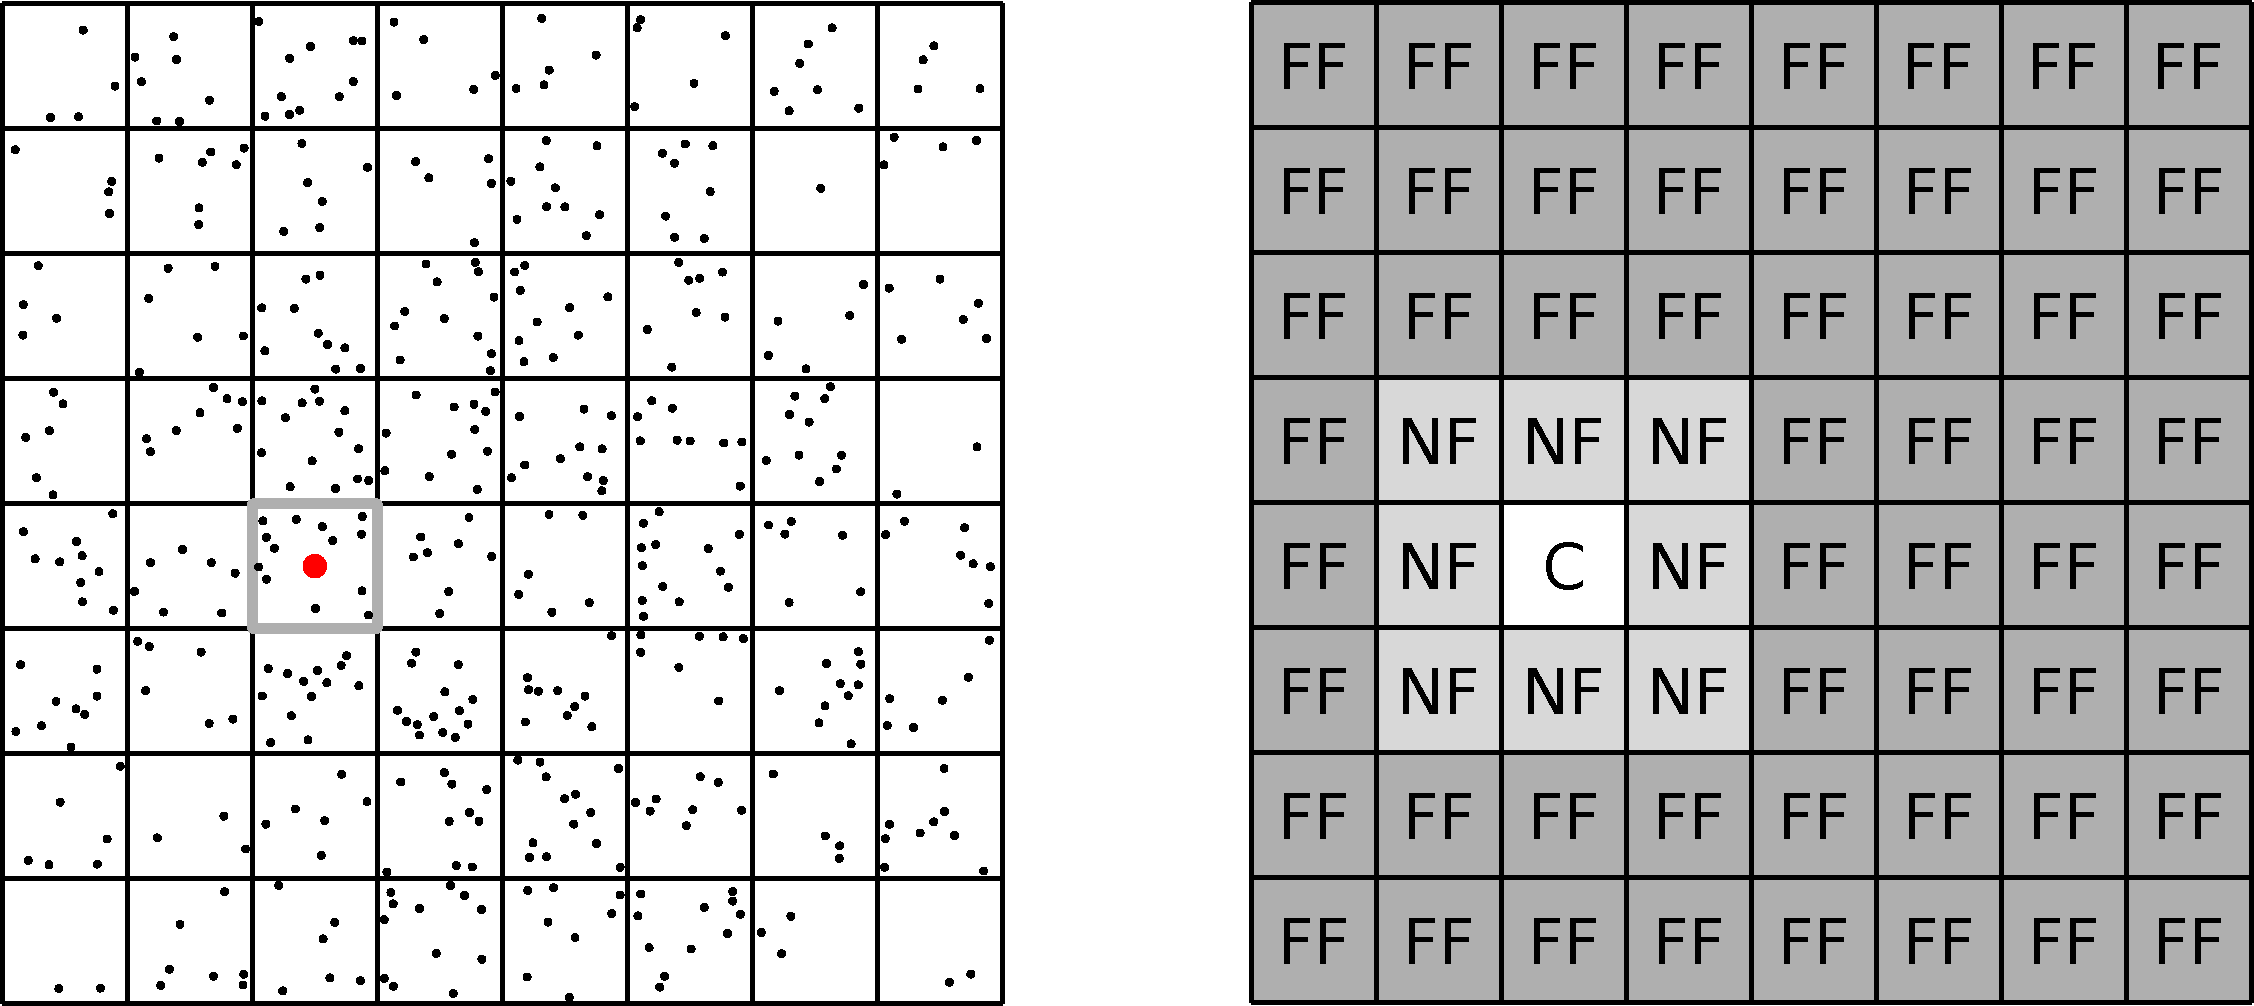
\includegraphics[scale=0.35]{Pics/FMM1}
\caption[Single-level multipole method]{In multipole methods, the system is subdivided into blocks of equal size containing one or more particles. For a reference block $C$, its surrounding blocks are categorized into near-field and far-field contributions which are treated using separate methods.}
\label{fig:FMM1}
\end{figure}

\begin{figure}
\centering
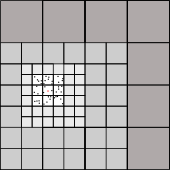
\includegraphics[scale=0.35]{Pics/FMM2}
\caption[Fast multipole method]{In the fast multiple method, the granularity of the boxes becomes coarser the further away they are from the source blocks.}
\label{fig:FMM2}
\end{figure}

% Ark1970 https://www.sciencedirect.com/book/9780123846549/mathematical-methods-for-physicists
% Gre1987 L. Greengard and V. I. Rokhlin, J. Comput. Phys. 73, 325 (1987)
% Gre1994 L. Greengard, Science 265, 909, (1994)
% Din1992 H. Q. Ding, etc.... look at 28, 29 p. 426 big book

\subsection{Continuous Fast Multipole Method}

The fast multipole method does not work for continuous charge distributions like Gaussian functions, as their extents can be quite different from one another, making the separation into NF and FF contributions more difficult. Nonetheless, FMM has been generalized to the continuous case, known as the continuous fast multipole method (CFMM) \cite{Whi1996}. The principle is the same as in multi-level multipole methods, only special care needs to be taken to only include classical contributions into the FMM treatment. For further details, the reader is referred to the original publication. 

\section{The ABCs of LMOs and NOs: Orbital Representations \label{sec:ABCLMO}}

To efficiently solve the Hartree-Fock equations, it is favorable to choose the set of molecular orbitals such that they diagonalize the Fock matrix $\mbf{F}$. In other words, they are eigenfunctions of the Fock operator
\begin{equation}
\hat{f}\sket{\phi_i} = \eps_i \sket{\phi_i}
\end{equation} 
\noindent Here, $\{\phi_i\}$ are also known as the \emph{canonical molecular orbitals}. CMOs are not unique in the sense that there are infinitely many alternative molecular representations which yield the same electron density $\mathbf{P}$. Quantities like the total wave function energy or the electronic density are said to be \emph{orbitally invariant}. Non-observables like the MO energies are not preserved under orbital rotation. Let $\mbf{C}$ be the CMO coefficient matrix. A new solution to the HF equations can then be generated by applying a unitary transformation such that
\begin{equation}
C^{new}_{\mu \olj} = U_{ji} C_{\mu i} \qquad \mbf{UU}\pdg = \mbf{1}
\end{equation} 
\noindent There are different reasons why one would want to use another MO basis: they can (a) offer a more intuitive picture for the interpretation of chemical phenomena and (b) help to achieve are more localized and compact representation of the wave function which is helpful for local correlation methods.

There are two significant types of molecular representations besides CMOs: local molecular orbitals (LMOs) and natural orbitals (NOs). The following sections will introduce both  types in more detail.

\subsection{Local Molecular Orbitals}

In contrast to canonical molecular orbitals, which are generally delocalized over the whole molecule, local molecular orbitals are confined to a relatively small volume and span only a few atoms (except in large conjugated systems). LMOs are well suited for a qualitative description of chemical reaction in terms of molecular bonds, lone pairs and $\pi$ systems \cite{Ste2019}. Moreover, they are often used in local correlation methods due to their reduced orbital span. There are several different ways for generating LMOs.

\subsubsection{LMOs by Reducing a Functional}
% (0) https://aip.scitation.org/doi/full/10.1063/1.2360264
% (1) https://journals.aps.org/rmp/abstract/10.1103/RevModPhys.32.296
% (2) https://journals.aps.org/rmp/abstract/10.1103/RevModPhys.35.457
% (3) https://aip.scitation.org/doi/10.1063/1.456588
% (4) J. E. Subotnik, Y. Shao, W. Z. Liang, and M. Head-Gordon, J. Chem. Phys. https://doi.org/10.1063/1.1790971 121, 9220 (2004).
% (5) https://aip.scitation.org/doi/10.1063/1.2033687

One of the most popular methods for finding LMOs consists in maximizing a localization function $\eta(\phi)$ by successive rotation of the orbital space. The most prominent examples are Foster-Boys (FB) \cite{Boy1960}, Edmiston-Ruedenberg (ER) \emph{Edm1963} and Pipek-Mezey (PM) \cite{Pip1989}. Their functionals can be written as

\begin{eqnarray}
\zeta_{FB}(\chi) = \sum_i \bra{\chi_i} \mathbf{r} \ket{\chi i}^2 \\
\zeta_{ER}(\chi) = \sum_i \cn{\chi_i \chi_i}{\chi_i \chi_i} \\
\zeta_{FB}(\chi) = \sum_i \sum_A \bra{\chi_i} \mathbf{P}_A \ket{\chi i}^2 
\end{eqnarray}

The problem is generally solved using an iterative procedure consisting in consecutive pair-wise rotations, known as Jacobi sweeps. These sweeps are repeated until convergence is reached, which may be slow. The methods differ within the procedure by how the rotational angle is computed, and scale differently with system size, with $\ccpx{3}$ for FB, $\ccpx{5}$ for ER and $\ccpx{4}$ for PM. A faster alternative to Jacobi sweeps does also exist \cite{Sub2004}. 

Over the years, PM has been the more popular choice of the three: like ER and unlike FB, it conserves $\sigma$-$\pi$ separation \cite{Aqu2006}, but scales more favorably than ER.

Functional localization methods are most often used for rotating occupied MOs. Virtual MOs are often plagued by convergence issues and have a steep computational cost simply due to being much more numerous than occupied MOs \cite{Sub2005}. It is crucial that molecular localization should not take longer than the methods they are used for, and hence VMOs are often localized using separate methods (e.g. PAO).

% EXAMPLES!! Ethylene (?)

\subsubsection{Projected Atomic Orbitals \label{sec:PAO}}
% (0) https://www.annualreviews.org/doi/10.1146/annurev.pc.44.100193.001241
% (1) https://aip.scitation.org/doi/full/10.1063/1.2173249

A set of highly localized molecular orbitals can be obtained by projecting the CMOs onto the atomic orbital basis, known as projected atomic orbitals (PAO) \cite{Sae1993}. For a set of orthonormal occupied and virtual molecular orbitals $\{\Psi_i\}$ and $\{\Psi_a\}$, the projection operators $\hat{P}$ and $\hat{Q}$ are defined as \cite{Chr2006}

\begin{eqnarray}
\hat{P} &= \sket{\Psi_i} \sbra{\Psi_i} &= \sket{\chi_{\mu}} C_{\mu i} C_{\nu i} \bra{\chi_{\nu}} \\
\hat{Q} &= \sket{\Psi_a} \sbra{\Psi_a} &= \sket{\chi_{\mu}} C_{\mu a} C_{\nu a} \sbra{\chi_{\nu}}
\end{eqnarray}

\noindent which are then applied to the atomic orbitals $\chi$ 

\begin{eqnarray}
\hat{P} \sket{\chi_{\mu'}} &= \sum_{\mu} P_{\mu\nu} S_{\nu\mu'} \sket{\chi_{\mu'}} &= \sum_{\mu} \ovl{P}_{\mu \mu'} \sket{\chi_{\mu'}} = \sket{\chi_{\ulgm}} \\
\hat{Q} \sket{\chi_{\mu'}} &= \sum_{\mu} Q_{\mu\nu} S_{\nu\mu'} \sket{\chi_{\mu'}}  &= \ovl{Q}_{\mu \mu'} \sket{\chi_{\mu'}} = \sket{\chi_{\olgm}}
\end{eqnarray} 

The projection operators $\hat{P}$, $\hat{Q}$ and the non-symmetric PAO coefficient matrices $\mathbf{\ovl{P}}$, $\mathbf{\ovl{Q}}$ are \emph{idempotent}
\begin{equation}
\mbf{\ovl{P}}\mbf{\ovl{P}} = \mbf{\ovl{P}} \qquad
\mbf{\ovl{Q}}\mbf{\ovl{Q}} = \mbf{\ovl{Q}}
\end{equation}

\noindent and \emph{mutually orthogonal} 
\begin{equation}
\mbf{\ovl{P}}\mbf{\ovl{Q}} = \mbf{0} \qquad \mbf{\ovl{P}} + \mbf{\ovl{Q}} = \mbf{1} 
\end{equation} 

\noindent but not orthogonal within themselves
\begin{equation}
\sbraket{\chi_{\ulgm}}{\chi_{\ulgn}} = S^{PAO}_{\ulgm\ulgn} \qquad \sbraket{\chi_{\olgm}}{\chi_{\olgn}} = S^{PAO}_{\olgm\olgn}
\end{equation}
\noindent Here, the indices $\ulgm,\ulgn,...$ and $\olgm,\olgn,...$ are used for occupied and virtual projected atomic orbitals, respectively. The number of PAOs (occupied or virtual) is equal to the number of AOs, and are therefore linearly dependent (redundant). CMOs are transformed to PAOs by using
\begin{eqnarray}
\sket{\chi_{\ulgm}} &= (\mathbf{SC})_{\mu i}  \sket{\Psi_i} &= \ovl{C}_{\mu i} \ket{\Psi_i} \\
\sket{\chi_{\olgm}} &= (\mathbf{SC})_{\mu a} \sket{\Psi_a} &=  \ovl{C}_{\mu a} \ket{\Psi_a}
\label{CMO2PAO}
\end{eqnarray}
\noindent The back-transformation is defined as
\begin{eqnarray}
\sket{\Psi_{i}} &= C_{\mu i} \sket{\ulgm} \\
\sket{\Psi_{a}} &= C_{\mu a} \sket{\olgn} 
\label{PAO2CMO}
\end{eqnarray}
PAOs are centered on the atom on which their corresponding AO is localized, but can still be delocalized over multiple atoms, depending on the sparsity of the density matrix. Methods which are entirely formulated in PAOs are rare but possible \cite{Chr2006}. The projection method is most often used on the virtual orbital space, where standard localization procedures fail. In literature, the following alternative formula is often used for expression the virtual PAO coefficient matrix in terms of the occupied LMOs:
\begin{equation}
\mbf{\ovl{Q}} = \left( \mbf{1} - \mbf{LL}^{\dagger} \mbf{S} \right) \mbf{C} 
\end{equation}
\noindent where $\mbf{L}$ is the coefficient matrix of the occupied LMOs.

\subsubsection{Cholesky Molecular Orbitals}

Sparsity of the atomic density matrix is crucial for achieving low-scaling electronic structure methods. Aquilante et al. proposed \cite{Aqu2006} to define a set of occupied molecular orbitals by Cholesky decomposition of the density matrix. Analysis of the resulting Cholesky molecular orbitals (CholMOs) showed their localized character inherited from the sparsity of the density matrix.
\begin{equation}
\mathbf{P} = \mathbf{LL^T}
\end{equation}
Figure \ref{fig:LOCORB_CHOL} shows the sparsity of the occupied density matrix and the occupied Cholesky molecular coefficient matrix of the linear alkane H$_{322}$C$_{160}$. The number of CholMOs is equal to the rank of the density matrix, which is equal to the number of occupied orbitals. The CholMOs are computed by an incomplete Cholesky decomposition with full row and column pivoting (Section \ref{sec:CHOLDEC}). The unitary transformation matrix is given by

\begin{equation}
U_{i\uli} = C_{\mu i} S_{\mu \nu} L_{\nu \uli}
\end{equation}

The decomposition algorithm scales with $\ccpx{3}$ but can be made linearly scaling by using sparse matrix algebra. CholMOs have several advantages: the Cholesky decomposition is fast and non-iterative, and an initial guess for molecular orbitals is not needed. 

The scheme can be extended to virtual orbitals as well, by CD of the virtual atomic density matrix $\mathbf{Q}$. The rank of $\mathbf{Q}$ is equal to the number of virtual orbitals $n_{vir}$, therefore the prefactor of the incomplete CD increases with basis set size. Especially in the presence of diffuse functions, the rank reduction might not offer much of an advantage compared to simpler localization methods such as PAOs.  

Moreover, orbitals obtained by CD are less localized than FB or ER LMOs, especially for small molecules. Low scaling is still possible using CholMOs in the context of LMO correlation methods, albeit with a larger prefactor.

CD is also used in the context of AO-MP2 to reduce the prefactor of integral transformation by using the rank sparsity of the pseudo-density matrices, as will be shown further below. CholMOs can also used as an initial guess for iterative localization schemes to achieve faster convergence.

\begin{figure}[ht]
\centering
\begin{subfigure}{0.5\linewidth}
\centering
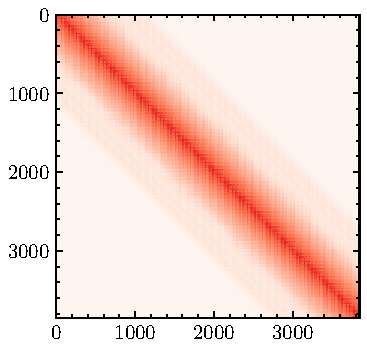
\includegraphics[scale=1.0]{Pics/densityO}
\end{subfigure}
$\Longrightarrow$
\begin{subfigure}{0.4\linewidth}
\centering
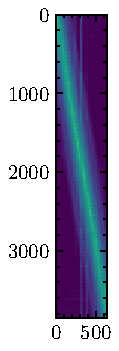
\includegraphics[scale=1.0]{Pics/choleskyO}
\end{subfigure}%
\hfill
\centering
\begin{subfigure}{0.5\linewidth}
\centering
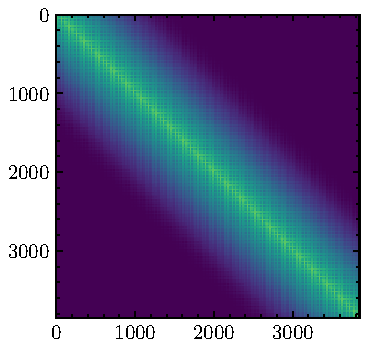
\includegraphics[scale=1.0]{Pics/densityV}
\end{subfigure}
$\Longrightarrow$
\begin{subfigure}{0.4\linewidth}
\centering
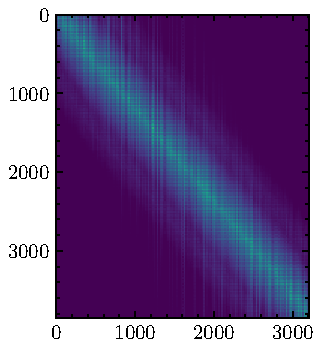
\includegraphics[scale=1.0]{Pics/choleskyV}
\end{subfigure}%
\caption[Cholesky decomposition of density matrices]{Cholesky decomposition of the occupied and virtual density matrices (left) yields a set of coefficients that describe a localized MO basis in the orbital and virtual space, respectively (right). The matrices are represented in terms of a heat map which indicates the magnitude of $\mathrm{log}_{10}(\mathrm{abs}(a_{ij}))$.}
\label{fig:LOCORB_CHOL}
\end{figure} 

\subsection{Natural Orbitals}

While the schemes described above try to generate a set of occupied and/or virtual molecular orbitals localized in space, natural orbital (NOs) methods try to generate a set of "compact" orbitals, i.e. a minimal set of orbitals that can describe the problem at hand. The concept of natural orbitals was first introduced by Löwdin \cite{Low1956}. The natural orbitals $\Theta_i$ of a wave function $\Psi$ are defined as the eigenfunctions of the one-particle density operator $\hat{n}$

\begin{equation}
\hat{n}\ket{\Theta_i} = n_i \ket{\Theta_i} 
\end{equation}

\noindent where $n_i$ are the occupation numbers of the associated orbital $\Theta_i$. One can then choose a reduced orbital space $\{\tilde{\Psi}_i\}$ by only taking into account those orbitals with an occupation number above a certain threshold $\tau$. The orbitals are "natural" in the sense that they are determined purely using $\Psi$, and are intrinsic to the system. NOs are computed by diagonalizing the one-particle density matrix at the desired level of theory (Hartree-Fock, MP, CIS, CC). 

%NOs are state-specific (Pok2019), meaning that NOs computed from the ground state densities may not be well suited to describe excited states, and NOs of different excited states might also greatly differ. As such, as will be later shown for local flavours of ADC, NOs need to be recomputed for each state.

% CIS(D) density matrices https://aip.scitation.org/doi/pdf/10.1063/1.4983277

\subsubsection{Natural Orbitals in Hartree Fock Theory}

In Hartree-Fock theory, natural orbitals are mostly reserved for qualitative population and bond order analysis. 

Natural atomic orbitals (NAOs) are computed by diagonalizing the blocks $P_{\mu_A\nu_A}$ of the atomic density matrix, where ${\mu_A}$, ${\nu_A}$ are basis functions centered on atom $A$. NAOs are optimal for describing the electron density around individual atom centers. NAOs are also useful for obtaining a set of guess orbitals from density matrices formed from the superposition of atomic densities (SAD) guess (Appendix \ref{sec:SCFGUESS}). 

Furthermore, NAOs serve as the starting point for obtaining natural hybrid orbitals (NHOs), which in turn are used for constructing natural bond orbitals (NBOs). NBOs are a useful orbital representation for  analyzing molecular bonds (e.g. bond order, bond polarity). They are conceptually close to the traditional Lewis structure of a molecule \cite{Ree1983,Wei2001,Gle2012}.

% (ref: https://pubs.acs.org/doi/pdf/10.1021/ja00544a007)
% NBOs https://aip.scitation.org/doi/pdf/10.1063/1.445134
% NAOs, NBOs https://pubs.rsc.org/en/content/articlepdf/2001/rp/b1rp90011k
% (Recent) NBOs https://onlinelibrary.wiley.com/doi/epdf/10.1002/wcms.51
% https://goldbook.iupac.org/terms/view/NT07076

\subsubsection{Frozen Natural Orbitals}

For large basis sets, the number of occupied canonical MOs is several times lower than the number of virtual canonical orbitals. Furthermore, NOs do not considerably reduce the number of occupied orbitals. It is therefore sufficient to only compute the eigenfunctions of the virtual-virtual block of the one-particle density matrix, in what is known as the frozen natural orbitals (FNOs) approach \cite{Bar1970}. FNOs need information of the correlated wave function, and are therefore typically computed at a lower level of theory. For example, the easiest way to obtain a set of FNOs for CCSD or CCSD(T) computation is to diagonalize the virtual-virtual block  of the MP2 density matrix \cite{Sos1989, Tau2005, Tau2008}
\begin{equation}
D_{ab} = \frac{1}{2} \sum_{cij} \frac{K_{ij}^{cb} K_{ij}^{ca}}{\eps_{ij}^{ab} \eps_{ij}^{ca}}
\end{equation}
\noindent with
\begin{equation}
K_{ij}^{ab} = 2 \cn{ia}{jb} - \cn{ib}{ja}
\end{equation}
\begin{equation}
\eps_{ij}^{ab} = \eps_i + \eps_j - \eps_a - \eps_b 
\end{equation}
The FNOs are then canonicalized. The combined set of occupied CMOs and virtual FNOs forms a very compact representation suitable for CC ground state and excited state calculations.

% MP2 NOs:
% Jor1988 J. Chem. Phys. 88, 3834 (1988); https://doi.org/10.1063/1.453884
% D. M. Silver and R. J. Bartlett,Phys. Rev. A13,1 1976.
% D. M. Silver, S. Wilson, and R. J. Bartlett,Phys. Rev. A16,477 1977.

% FNOs: 
% Bar1970 Phys. Rev. A 1, 644 – Published 1 March 1970

% FNO CC: 
% Sos1989 https://doi.org/10.1016/0009-2614(89)87399-3
% Tau2005 Taube, Andrew G.; Bartlett, Rodney J. (2005). Frozen Natural Orbitals: Systematic Basis Set Truncation for Coupled-Cluster Theory. Collection of Czechoslovak Chemical Communications, 70(6), 837–850. doi:10.1135/cccc20050837  
% A. G. Taube and R. J. Bartlett,  Frozen natural orbital coupled-cluster theory:  Forces andapplication to decomposition of nitroethane,  J. Chem. Phys.128, 164101 (2008)
% CCLR NO  A. Kumar and T. D. Crawford,   Frozen virtual natural orbitals for coupled-cluster linear-response theory,  J. Phys. Chem. A121, 708 (2017).

% Have a look at Pok2019 https://chemrxiv.org/articles/preprint/Extension_of_Frozen_Natural_Orbital_Approximation_to_Open-Shell_References_Theory_Implementation_and_Application_to_Single-Molecule_Magnets/10308053/1

\subsubsection{Natural Transition Orbitals}

Consider the CIS eigenvalue problem for finding the excitation energies $\omega_n$ and their associated transition density matrices $\mbf{R}_n$

\begin{equation}
\mathbf{A_{CIS}} \mbf{R}_n = \omega_n \mbf{R}_n 
\end{equation}

\noindent The matrices $\mathbf{R}_n$ contain $n_{occ}n_{vir}$ expansion coefficients $c_{ia}$ which show how much an orbital-virtual MO pair $ia$ contributes to the excitation $n$. The number of non-negligible coefficients can be far from zero, making interpretations of the computed results difficult for some systems.

Natural transition orbitals (NTOs) were introduced to facilitate the qualitative description of an excited state and finding connections to experimental spectra \cite{Luz1976, Mar2003}. NTOs are typically obtained by computing the singular value decomposition (SVD) of the state densities $\mathbf{R}_n$

\begin{equation}
\mathbf{R} = \mathbf{U} \mathbf{\Sigma} \mathbf{V}^{\dagger}  
\end{equation} 

\noindent where $\mathbf{U}$ and $\mathbf{V}$ are unitary matrices with dimension $n_{occ} n_{NTO}$ and $n_{vir}n_{NTO}$, and $\Sigma$ is a $n_{NTO}$ by $n_{NTO}$ matrix containing the singular values $s$ on its diagonal. The CMOs $\{\Psi^{occ}_i,\Psi^{vir}_a\}$ are transformed to the NTO basis $\{\overline{\Psi}^{occ}_k,\overline{\Psi}^{vir}_k\}$ using

\begin{equation}
\ket{\overline{\Psi}^{occ}_k} = U_{ki} \ket{\Psi^{occ}_i}
\end{equation}
\begin{equation}
\ket{\overline{\Psi}^{vir}_k} = V_{ka} \ket{\Psi^{vir}_a}
\end{equation}

\noindent The singular value $s_k$ show the contribution of an NTO pair $k$ to the excited state. In most cases, the number of significant NTO pairs is significantly lower than $n_{occ}n_{vir}$ and at most equal to $n_{occ}$. NTOs are not limited to CIS, but can also be obtained by SVD decomposition of the singles-singles block of excited state densities from higher order methods such as ADC or CCLR. 

Natural transition orbitals have also found use in local excited  state correlation methods \cite{Bau2017,Hof2017}, where CIS NTOs are combined with MP2 NOs to obtain a compact orbital representation for ground and excited state coupled cluster calculations.

%EXAMPLE!!! phenylalanine

% Luz1976 https://link.springer.com/article/10.1007%2FBF00526670

% Mar2003 https://aip.scitation.org/doi/pdf/10.1063/1.1558471

% https://www.sciencedirect.com/science/article/pii/S0009261407002072?via%3Dihub

% CornFlex: Bau2017 https://aip.scitation.org/doi/pdf/10.1063/1.4984820

% Hof2017 Natural transition orbitals for the calculation of correlation andexcitation energies

\subsection{Specific Virtual Orbitals}

In most cases, using LMOs instead of CMOs does not offer any a priori advantage in terms of the computational complexity associated with correlated methods, and additional approximations are necessary. In local correlation methods, this is often done by truncating the VMO space. Truncation of the VMOs has been an active field of research for several decades. A naive approach to truncate the virtual space would be to eliminate VMOs with orbital energies above a certain threshold; however, this proved to be unusable in most contexts \cite{Sen2011}. More successful methods for VMO truncation use the concept of what will referred to as \emph{specific virtual orbitals} (SVOs). SVOs are specific in the sense that each individual occupied MO $i$ or each pair of MOs $ij$ has their own set of SVOs $a_i$ (orbital specific virtual orbitals) or a$_{ij}$ (pair specific virtual orbitals) associated to it.
The concept of SVOs naturally arises in the context of correlated methods such as the coupled electron pair approximation (CEPA) where the total energy is computed is computed as the sum of electron pair energies $e$
\begin{equation}
E_{CEPA} = \sum_{ij} e_{ij}
\end{equation}
The electron pair energy decays rapidly as a function of the distance $r$ between MO centers in an LMO basis. Distant virtual orbitals contribute less to the electron pair energy as virtual orbitals close to ${ij}$. It has been shown early on that instead of using the whole virtual orbital span, one can correlate only a subset or reduced set of virtual orbitals with each electron pair \cite{Sae1985,Edm1965,Mey1971,Mey1973}
%(0,1,2,3) 
and still recover most of the correlation energy. In the limit of large molecules, the number of significant virtual orbitals for an electron pair becomes independent of system size \cite{Kra2012} (see also Chapter 4). There are different ways to choose how to define the VMO subsets, either by using local molecular orbitals or natural orbitals.

% 0 BASIS FOR LMO-PAO S. Saebø and P. Pulay , Chem. Phys. Lett., 1985, 113 , 13
% 1 BASIS FOR PNOs Edmiston, C.; Krauss, M. Configuration-interaction calculation of H3 and H2. J. Chem. Phys. 1965, 42, 1119– 1120,  DOI: 10.1063/1.1696050 
% 2 OTHER Meyer, W. Ionization energies of water from PNO-CI calculations. Int. J. Quantum Chem. 1971, 5, 341– 348,  DOI: 10.1002/qua.560050839 
% 3 ALSO Meyer, W. PNO-CI Studies of electron correlation effects. I. Configuration expansion by means of nonorthogonal orbitals, and application to the ground state and ionized states of methane. J. Chem. Phys. 1973, 58, 1017– 1035,  DOI: 10.1063/1.1679283
% 4 https://pubs.rsc.org/am/content/articlehtml/2012/cp/c2cp40231a#cit51

\subsubsection*{Domain Specific Virtual Orbitals}

The term \emph{domain specific virtual orbitals} (DSVOs) will be used to denote any type of virtual orbitals where the subsets are formed \emph{a priori} by distance or partial charge criteria. Examples include the local MP2 and local CCSD implementations by Schütz et al. \cite{Sch1999,Sch2001,Sch2000}.%(AA,AB,AC)

First, occupied CMOs are localized by one of the methods described above, e.g. FB or ER. Virtual CMOs are transformed into the PAO basis. Each individual occupied LMO $\ket{\Psi_i}$ is then assigned a subset $[i]$ of PAOs, chosen by a Boughton-Pulay (BP) criterion \cite{Bou1993} or by population analysis \cite{Mat2008}. For a given electron pair $ij$, the pair domain is then formed by taking the union $[ij]$ = $[i] \cup [j]$. The set of all virtual pair domains $[ij]$ forms the DSVOs.

Alongside AOs, DSVOs were among the first orbital representations in which linear scaling correlated methods were formulated. Their dependency on distance criteria for selecting the pair domains makes them less rigorous than other methods, and pure LMO+PAO methods have fallen somewhat out of favor over the years. Nonetheless, the concepts of local domains remain crucial for low-scaling algorithms using natural orbitals \cite{Rip2013}.

% Local LMO-PAO
% AA M. Schütz , G. Hetzer and H.-J. Werner , J. Chem. Phys., 1999, 111 , 5691
% AB M. Schütz and H.-J. Werner , J. Chem. Phys., 2001, 114 , 661
% AC M. Schütz and H.-J. Werner , Chem. Phys. Lett., 2000, 318 , 370 
% AD https://onlinelibrary.wiley.com/doi/abs/10.1002/jcc.540140615
% AE R. A. Mata, H.-J. Werner, S. Thiel and W. Thiel, J. Chem. Phys., 2008, 128, 025104

\subsubsection*{Pair Natural Orbitals}
% Review: https://pubs.rsc.org/am/content/articlehtml/2012/cp/c2cp40231a
First introduced under the guise of "pseudo-natural orbitals" \cite{Edm1965}, then rediscovered by Neese \cite{Nee2009a,Nee2009b,Han2011}, pair natural orbitals (PNOs) have risen in popularity in the recent years. Similarly to DSVMOs, each electron pair has a set of PNOs associated to it. PNOs are formed by diagonalizing the MP2 pair density matrix for each MO pair $ij$ (hence "pair-natural")

\begin{equation}
\mathbf{D}^{ij} = \frac{1}{1+\delta_{ij}} \left(\tilde{\mathbf{t}}^{ij} \mathbf{t}^{ij} + \tilde{\mathbf{t}}^{ij} \mathbf{t}^{ij\dagger} \right)
\end{equation}

\noindent with 

\begin{equation}
\mathbf{\tilde{t}}^{ij}_{ab} = 2 \mathbf{t}^{ij}_{ab} - \mathbf{t}^{ji}_{ab} 
\end{equation}

\noindent The eigenvalue decomposition of $\mathbf{D}$ then gives

\begin{equation}
\mathbf{D}^{ij} \mathbf{Q}^{ij} = n^{ij} \mathbf{Q}^{ij} 
\end{equation}

\noindent where $\mathbf{Q^{ij}}$ are the pair specific transformation matrices, and $n^{ij}$ their occupation numbers. The Fock matrix in the LMO representation is not diagonal, and the MP2 amplitudes are approximated by

\begin{equation}
t_{ij}^{ab} = \frac{\cn{ia}{jb}}{\eps_a + \eps_b - f_{ii} - f_{jj}}
\end{equation}

\noindent where $f_{ii}$ are the diagonal entries of the Fock matrix in the LMO basis. The pair domains $[ij]$ are chosen by keeping the PNOs with an occupation number larger than a threshold $\tau_{PAO}$. Therefore, accuracy is controlled by a single, distance-independent parameter, which is an advantage over other methods like DSVOs. 

However, computing the PNOs requires a full MP2 calculation, and with density fitting scales with $\ccpx{5}$. Moreover, even if the PNO basis is compact, the fact that each LMO pair has its own virtual orbital basis may lead to a prohibitively large number of PNOs for large molecules. The concept of PNOs can be combined with the domain-based approach of LMO+PAO, in what is known as local pair-natural orbitals (LPNOs) \cite{Rip2013}. 

% CA F. Neese, F. Wennmohs and A. Hansen, J. Chem. Phys., 2009, 130, 114108 CrossRef .
% CB F. Neese, A. Hansen and D. G. Liakos, J. Chem. Phys., 2009, 131, 064103 CrossRef .
% CC A. Hansen, D. G. Liakos and F. Neese, 2011, 135, 214102.

%Local PNOs:
% https://aip.scitation.org/doi/10.1063/1.4773581

\subsubsection*{Orbital Specific Virtuals}

Closely related to PNOs are the orbital specific virtual orbitals (OSVs) \cite{Yan2011}. The OSVs for an LMO $\ket{\Psi_i}$ are obtained by taking the diagonal PNOs for the domain $[ii]$. The MP2 density matrix reduces to

\begin{equation}
\mathbf{D}^{ii} = 4 \mathbf{t}^{ii} \mathbf{t}^{ii}
\end{equation}

\noindent Instead of reducing the density matrix, one can just diagonalize $\mathbf{t}^{ij}$ instead. 

\begin{equation}
\mathbf{t}^{ii} \mathbf{Q}^{ii} = t^{ii} \mathbf{Q}^{ii}
\end{equation}

\noindent where $t^{ii}$ are the eigenvalues, which are used to compute the compute the occupation numbers $n^{ii} = \left( t^{ii} \right)^2$. OSVs for which $n^{ii} > \tau_{OSV}$ are included into the orbital specific domain $[i]$. Pair domains $[ij]$ are then formed as the union of $[i]$ and $[j]$ similar to DSVOs. 

OSVs have the advantage that they can be constructed with $\ccpx{3}$ scaling provided that density fitting is used. However, OSVs are less compact than PNOs, but they can be used to lower the computational complexity to construct PNOs. Several hybrid OSV-PNO schemes have been proposed with a computational complexity of $\ccpx{4}$ \cite{Kra2012}, $\ccpx{3}$ \cite{Sch2013} and finally $\mathcal{O}(N)$ \cite{Rip2013}.

%\subsubsection{Local Pair Natural Orbitals}

% Rip2013 https://aip.scitation.org/doi/pdf/10.1063/1.4773581

%NAFs: \url{https://aip.scitation.org/doi/full/10.1063/1.4905005}
% DLPNO: relationship between i and X https://aip.scitation.org/doi/pdf/10.1063/1.4926879



\chapter{Local Correlation Methods (II): Ground State \label{cha:LOCAL1}}

Since the seminal work of S{\ae}b{\o} and Pulay \cite{Pul1983,Sae1985,Sae1993}, demonstrating how the computational effort of electronic structure methods may be reduced via a local treatment of electron correlation using LMOs and PAOs, the concept of locality has been applied to Hartree-Fock, M{\o}ller-Plesset and Coupled-Cluster methods. Over the years, pure LMO methods have somewhat fallen out of use, in favor for an atomic orbital or (local) natural orbital treatment. This chapter summarizes how the tools and concepts of sparsity and local electron correlation presented in the previous chapter can be used to reduce the scaling of electronic structure methods. The focus will mainly be on Hartree-Fock and M{\o}ller-Plesset, with some words on Coupled-Cluster as well.

\section{Low-Scaling Self-Consistent Field Methods}

Hartree-Fock and density field theory, grouped under the umbrella term of self-consistent field (SCF) methods, are the working horses in quantum chemistry, and the underlying equations, the Roothan and Kohn-Sham equations, are well known and studied. Conventional formulations of HF and DFT, without inclusion of sparsity, scale with $\ccpx{3}$ to $\ccpx{4}$ which hampers extension to very large systems. There are three major bottle-necks: (1) computation of the coulomb matrix, (2) computation of the exchange matrix and (3) diagonalization of the Fock matrix. Over the last couple of decades, multiple different approaches have been proposed on how to lower the scaling of constructing the Fock matrix and circumvent matrix diagonalization. To this day, the field of low scaling SCF methods remains an active area of research in theoretical chemistry. The next sections will address the time-determining steps in detail.

\subsection{The Coulomb Matrix}

Consider again the expression for the coulomb matrix $\mathbf{J}$ 
\begin{equation}
J_{\mu\nu} = \cn{\mu\nu}{\lambda\sigma} P_{\sigma\lambda}
\end{equation}
\noindent which gives the following sparsity diagram:

\begin{center}
\begin{tikzpicture}

\snode{MU}{0,0}{\mu};
\snode{NU}{1,0}{\nu};
\snode{SIG}{2,0}{\sigma};
\snode{LAM}{3,0}{\lambda};

\draw[<->] (MU) -- (NU) node [midway, above] () {S};
\draw[<->] (SIG) -- (LAM) node [midway, above] () {P/S};

\end{tikzpicture}
\end{center}

\noindent The construction of $\mathbf{J}$ has an inherent computational complexity of $\ccpx{2}$, even though the number of non-zero elements scales linearly due to the overlap relationship between $\mu$ and $\nu$. Quadratic scaling algorithms are straight-forward to implement. The first method to construct $\mathbf{J}$ with $\mathcal{O}(N)$ effort was the continuous fast multipole method (CFMM) \cite{Whi1996}. For each element $\mu\nu$ the contributions $\sigma\lambda$ are split into near-field and far-field contributions. NF interactions are computed using standard integration techniques, while FF interactions are computed using multi-level multipole expansion. The linear scaling remains even if the density matrix is not sparse. Other tree-like algorithms were also proposed \cite{Str1996,Cha1996}. In all cases, computing the NF interactions are by far the most time-consuming step.

One way to speed up the evaluation of the non-classical contributions is by moving the contraction step with the density matrix into the underlying integral evaluation. By modifying the formulas for the Gaussian integrals, the explicit storage of the 2-electron repulsion integrals can be skipped which greatly increases computational efficiency \cite{Whi1996,Sha2000,Sha2001}. To this day, the \emph{J engine method}, in combination with CFMM, remains the most efficient way to evaluate the exact Coulomb matrix.

Alternatively, one may introduce the density fitting approximation. The Coulomb matrix is then evaluated in several steps via the intermediates $\mathbf{D}$ and $\mbf{C}$ as 
\begin{align}
J_{\mu\nu} &= C_{X\mu\nu} D_X \\
D_X &= \cn{Y}{\mu\nu} P_{\nu\mu} \\
C_{X\mu\nu} &= \cn{X}{Y}^{-1} \cn{Y}{\mu\nu}
\end{align}
\noindent The computational effort remains unchanged, with $\ccpx{2}$, but with a much lower prefactor, especially for larger, more diffuse basis sets \cite{Wei2002}. Furthermore, the integrals can be recomputed on the fly, and do not need to be explicitly stored. The inversion of the metric matrix $\cn{X}{Y}$ scales cubically, and dominates the cost of the DF approximation for large molecules. 

For large molecules, one could also consider using local density fitting, such as the atomic resolution of the identity or pair-atomic resolution of the identity. Unfortunately, LDF also only reduces the prefactor, rather than scaling. Furthermore, it is necessary to use the robust density fitting of the electron integrals (Equation \ref{eq:DUNLAP}) to recover quadratic scaling in the fitting error, due to the constraints imposed on the density fitting procedure. The Coulomb matrix is then expressed as
\begin{align}
J_{\mu\nu} &= \cn{\mu\nu}{X} b_X + c^Y_{\mu\nu} \left[ g_Y - \tilde{g}_Y \right] \\
g_X &= C^X_{\mu\nu} P_{\mu\nu} \\
\tilde{g}_X &= \cn{X}{Y} b_{Y} \\ 
\quad b_{X} &= C_{\mu\nu}^{X} P_{\mu\nu} 
\end{align}
\noindent The robust LDF-J approximation is evaluated at an effort similar to standard DF-J. The only advantages to LDF in this case pertain to the fitting procedure itself. It is no longer necessary to invert the 2c2e integral matrix $\cn{X}{Y}$, and the fitting coefficients $C_{\mu\nu}^{X}$ can be evaluated in linear scaling fashion. However, it has been demonstrated that using Dunlap's robust formula in combination with local metrics leads to "attractive electron" states where the SCF energy may converge to very high positive values \cite{Mer2013,Hol2014}. The reason is that the the two-electron integral tensor in the robust LDF approximation is no longer positive semidefinite, but \emph{indefinite}, which can lead to severe convergence problems. One way to circumvent this problem is to loosen the constraints on the density fitting procedure, or use a larger auxiliary basis set. In both cases, performance is compromised.  

As shall be shown in chapter \ref{cha:RESULTS}, quasi-robust density offers a better alternative to robust LDF-J methods, with similar sparsity and higher accuracy without the use of Dunlap's formula.

%MEMORY : ON-THE FLY

%POISSON? 
% MANBY, F. R., and KNOWLES, P. J., 2001,Phys.  Rev.Lett.,87,163001.
% MANBY, F. R., KNOWLES, P. J., and LLOYD, A. W., 2001,J. Chem. Phys.,115,9144.

% Str1996 Strain MC, Scuseria GE, Frisch MJ. Achieving linear scaling for the electronic quantum coulomb problem. Science 1996, 271:51–53.
% Cha1996 Challacombe M, Schwegler E, Alml ̈of J. Fast assem-bly of the Coulomb matrix: a quantum chemical treecode.J Chem Phys1996, 104:4685
% Mer2013 Merlot, P.; Kjæ rgaard, T.; Helgaker, T.; Lindh, R.; Aquilante,F.; Reine, S.; Pedersen, T. B.J. Comput. Chem.2013,34, 1486−96.
% Hollman, D. S.; Schaefer, H. F.; Valeev, E. F.J. Chem. Phys.2014,140, 064109.

\subsection{The Exchange Matrix}

\subsubsection{Exact Exchange}

The expression for the exchange matrix is given by 
\begin{equation}
K_{\mu\nu} = \cn{\mu\sigma}{\nu\lambda} P_{\lambda\sigma}
\end{equation}
\noindent In the section where sparsity diagrams were introduced, it was demonstrated that the indices of the exchange expression can be fully linked:
\begin{center}
\begin{tikzpicture}

\snode{MU}{0,0}{\mu};
\snode{NU}{3,0}{\nu};
\snode{SIG}{1,0}{\sigma};
\snode{LAM}{2,0}{\lambda};

\draw[<->] (MU) -- (SIG) node [midway, above] () {S};
\draw[<->] (SIG) -- (LAM) node [midway, above] () {P};
\draw[<->] (LAM) -- (NU) node [midway, above] () {S};

\end{tikzpicture}
\end{center}
\noindent The non-zero elements in $\mathbf{K}$ scale linearly and can be evaluated with $\mathcal{O}(N)$. This property was realized quite early on \cite{Sch1997}. However, a straight-forward implementation where the 4c2e integrals are directly contracted with the density matrix $\mathbf{P}$ using sparse matrix algebra does not give the desired results, when applying the standard $\ccpx{2}$ Schwarz-screening to $\cn{\mu\sigma}{\nu\lambda}$. To lower the scaling of electron integral evaluation, it is important to design a screening algorithm which imposes the P junction between $\sigma$ and $\lambda$ which in turn leads to only a linear increase in the number of bra-ket pairs. 

The ONX method by Schwegler \cite{Sch1997} was the first $\mathcal{O}(N)$ scheme for constructing the exchange matrix, but did not exploit permutational symmetry, which lead to a four fold increase in the prefactor. More competitive methods were proposed later, such as Linear Exchange (LinK) \cite{Och1998}, or symmetrized ONX (SONX) \cite{Sch2000} that could also be applied to small systems without major overhead.

For all approaches, an important step is the screening of the bra-ket pairs using a density-weighted integral estimate
\begin{equation}
|P_{\lambda\sigma}||\cn{\mu\sigma}{\mu\sigma}|^{1/2} |\cn{\nu\lambda}{\nu\lambda}|^{1/2} \leq \tau
\end{equation}
\noindent which scales linearly in the limit of large systems with large HOMO-LUMO gaps. Furthermore, shell ordering is very important to avoid the $\ccpx{2}$ complexity of screening and enable early exit out of the shell loops during construction of the exchange matrix. Similarly to the J kernel, the electron integrals need not to be held in memory, but can be recomputed on the fly.

% https://aip.scitation.org/doi/10.1063/1.472135
% Sch1997 https://aip.scitation.org/doi/10.1063/1.473833
% Och1998 https://aip.scitation.org/doi/10.1063/1.476741
% Sch2000 https://link.springer.com/article/10.1007%2Fs002140000127

\subsubsection{Density Fitting}

The downside of exact linear exchange algorithms is the steep $\ccpx{4}$ scaling with increasing basis set size which delays the onset of the low-scaling regime. For this reason, considerable effort has been invested in recent years to also exploit rank sparsity by density fitting. The DF expression for the exchange matrix in the AO basis reads
\begin{align}
C^X_{\mu\nu} &= \cn{X}{Y}^{-1} \cn{Y}{\mu\nu} \label{eq:DFAOK_STEP1}\\
K_{\mu\nu} &= C^X_{\nu\lambda} \cn{X}{\mu \sigma} P_{\sigma\lambda} \label{eq:DFAOK_STEP2}
\end{align}
\noindent In a straight-forward implementation using sparse matrix algebra, Equation \ref{eq:DFAOK_STEP1} and Equation \ref{eq:DFAOK_STEP2} are evaluated with $\ccpx{3}$  and $\ccpx{2}$ effort respectively. The non-zero elements of both the fitting coefficients $C$ and the 3c2e integrals increase quadratically. Their storage can quickly become problematic for large basis sets if both are held in-core. In principle, both tensors can be recomputed batchwise on-the-fly to reduce memory-footprint, but in contrast to the DF-J kernel where only the 3c2e integrals need to be generated at each iteration, recomputing the fitting coefficients each time introduces a prefactor that is too large for an out-of-core DF-K kernel to be of any practical use (see Chapter \ref{cha:RESULTS}).

For an efficient, direct evaluation of the exchange matrix using density fitting, an MO based approach is much more favorable \cite{Wei2002}. The MO-DF-K kernel is evaluated as
\begin{align}
B^{X}_{\mu i} &= C_{\nu i} \cn{X}{\mu\nu} \\
D^{X}_{\mu i} &= \cn{X}{Y}^{-1/2} B^{X}_{\mu i} \\
K_{\mu\nu} &= B^{X}_{\mu i} B^{X}_{\nu i}
\end{align}
\noindent with cubic computational complexity. The matrix elements of the exchange matrix are evaluated batch-wise over occupied blocks $I$. By contracting the 3c2e integrals with the coefficient matrix $C_{\mu i}$ to form the half-transformed integrals $B^X_{\mu i}$, storage can be reduced from $N_{aux} N_{AO}^2$ to $N_{aux} N_{AO} N_{occ} / N_I$. The 3c2e integrals need to be recomputed for each block $I$, but in practice the number of blocks can be held quite small. The DF-MO-K method is especially well suited for small to medium sized molecules with large diffuse basis sets for post-HF calculations.      

% Wei2002 https://pubs.rsc.org/en/content/articlehtml/2002/cp/b204199p

\subsubsection{Local Density Fitting}

Standard density fitting introduces long-range interactions which inhibit the linear scaling construction of the exchange matrix. This problem can be solved by using LDF. Again, Dunlap's robust density fitting needs to applied to get accurate results. The robust DF-K kernel can take the form
\begin{align}
E_{\mu\nu}^{X} &= C^{X}_{\mu\sigma} P_{\lambda\nu} \\
L_{\mu\nu} &= E_{\mu\sigma}^X \cn{X}{\nu\sigma} - \frac{1}{2} E_{\mu\sigma}^X \cn{X}{Y} C^{Y}_{\nu\sigma} \\
K_{\mu\nu} &= L_{\mu\nu} + L_{\nu\mu}
\end{align}
\noindent All steps can be evaluated in $\mathcal{O}(N)$ time, under the assumption that the fitting coefficients scale linearly:
\begin{center}
\begin{tikzpicture}
\snode{E}{0,0}{E:};
\snode{X}{1,0}{X};
\snode{MU}{2,0}{\mu};
\snode{SIGMA}{3,0}{\sigma};
\snode{NU}{4,0}{\nu};
\draw[<->] (X) -- (MU) node [midway, above] () {LDF};
\draw[<->] (MU) -- (SIGMA) node [midway, above] () {S};
\draw[<->] (SIGMA) -- (NU) node [midway, above] () {P};
\end{tikzpicture}
\end{center}
\begin{center}
\begin{tikzpicture}
\snode{L}{0,0}{L:};
\snode{X}{1,0}{X};
\snode{MU}{2,0}{\mu};
\snode{SIGMA}{3,0}{\sigma};
\snode{NU}{4,0}{\nu};
\snode{PLUS}{5,0}{+};
\snode{X1}{6,0}{X};
\snode{MU1}{7,0}{\mu};
\snode{SIGMA1}{8,0}{\sigma};
\snode{NU1}{9,0}{\nu};
\snode{Y}{10,0}{Y};
\draw[<->] (X) -- (MU) node [midway, above] () {LDF};
\draw[<->] (MU) -- (SIGMA) node [midway, above] () {P};
\draw[<->] (SIGMA) -- (NU) node [midway, above] () {S};
\draw[<->] (X1) -- (MU1) node [midway, above] () {LDF};
\draw[<->] (MU1) -- (SIGMA1) node [midway, above] () {P};
\draw[<->] (SIGMA1) -- (NU1) node [midway, above] () {S};
\draw[<->] (NU1) -- (Y) node [midway, above] () {LDF};
\end{tikzpicture}
\end{center}
\begin{center}
\begin{tikzpicture}

\snode{K}{0,0}{K:};

\snode{MU}{1,0}{\mu};
\snode{NU}{2,0}{\nu};
\snode{PLUS}{3,0}{+};
\snode{MU1}{5,0}{\nu};
\snode{NU1}{4,0}{\mu};

\draw[<->] (MU) -- (NU) node [midway, above] () {};
\draw[<->] (NU1) -- (MU1) node [midway, above] () {};
\end{tikzpicture}
\end{center}

\noindent Alternatively, an LDF-K scheme based on LMOs is also possible \cite{Pol2004,Mej2014}. Over the years, many different LDF-K kernels have been proposed that approximate $C_{\mu\nu}^X$ based on LMO domains \cite{Pol2004,Mej2014}, the atomic resolution of the identity (ARI) \cite{Sod2008}, the pair-atomic resolution of the identity (PARI) \cite{Mer2013} or the concentric atomic density fitting (CADF) \cite{Hol2017}. Although the electron integrals are no longer positive semidefinite, LDF-K is not plagued by the same convergence problems as LDF-J, and it has been shown that LDF-K can be combined with standard DF-J to circumvent convergence problems \cite{Man2015}. 

% Pol2004 https://www.tandfonline.com/doi/abs/10.1080/0026897042000274801
% Sod2007 Hartree-Fock exchange computed using the atomic resolutionof the identity approximation
% Mer2013 https://onlinelibrary.wiley.com/doi/10.1002/jcc.23284
% Mej2014 https://aip.scitation.org/doi/full/10.1063/1.4896199
% Man2015 https://pubs.acs.org/doi/abs/10.1021/ct5008586
% Hol2017 Fast construction of the exchange operator in an atom-centred basis with concentric atomic densityfitting

%\subsubsection{Other Methods}
%
%Other methods for linear-scaling evaluation of Hartree-Fock exchange (also often abbreviated as HFX in literature) are the semi-numerical chain-of-spheres methods (COS) \cite{Nee2009c,Izs2011} and the auxiliary density matrix methods (ADMM) \cite{Gui2010}. For further details, the reader is referred to the original publications. (Maybe elaborate?)

% COS Nee2009 https://www.sciencedirect.com/science/article/pii/S0301010408005089
% COS2 Isz2011 https://aip.scitation.org/doi/full/10.1063/1.3646921
% ADFMM Gui2010 https://pubs.acs.org/doi/10.1021/ct1002225

\subsection{The SCF Procedure}

In the standard SCF procedure, the construction of the Fock matrix is followed by a cubic scaling diagonalization to obtain the MO coefficient matrix and the MO energies. As was discussed in detail in the previous chapter, the eigenvectors of the Fock matrix, i.e. the canonical MOs, are delocalized, and therefore using a sparse eigenvalue solver is unfortunately not an option. The solution is to entirely avoid any MO quantities and replace the Fock diagonalization step. For a functional, fully AO-based method, the same constraints on the density matrix need to be fulfilled as in the standard SCF procedure:
\begin{alignat}{2}
\mathbf{P} &= \mathbf{P}^{\dagger} \qquad &\textrm{Hermiticity}
\\
Tr(\mathbf{PS}) &= N_{ele} \qquad &\textrm{$N$-representability}
\\
\mathbf{PSP} &= \mathbf{P} \qquad &\textrm{Idempotency}
\\
\mathbf{FPS} &- \mathbf{SPF} = \mathbf{0} \qquad &\textrm{Commutator}
\end{alignat}
\noindent There are two main approaches for replacing Fock matrix diagonalization: Purification (or spectral projection) and density matrix minimization \cite{Kim2016}. % (Jor2005).

In spectral projection methods, an initial guess for the density matrix $\mathbf{P}$ of its Fock matrix $\mathbf{F}$ is obtained as
\begin{equation}
\mathbf{P} = \Theta \left( \mu \mathbf{I} - \mathbf{F} \right)
\end{equation}
\noindent where $\mu$ is the chemical potential, and $\Theta$ is the Heaviside step-function. The guess density then has orbital occupation numbers spread between 0 and 1, and has the same eigenvectors as the Fock matrix. The idempotent density is then determined by \emph{density purification}. Density purification is an iterative procedure where a purification transformation is repeatedly applied to the density matrix which converges the orbital occupation numbers either towards 0 or 1. One of the earliest purification transformation by McWeeny \cite{McW1959} takes the form
\begin{equation}
\mathbf{P}_{n+1} = 3\mathbf{P}_n\mathbf{SP}_n - 2\mathbf{P}_n\mathbf{SP}_n\mathbf{SP}_n
\label{eq:MCWEENY}
\end{equation}
\noindent Equation \ref{eq:MCWEENY} is also known as the grand-canonical purification scheme. Other transformations have been proposed over the years, such as canonical purification \cite{Pal1998} or trace-resetting purification \cite{Nik2003}, which do not need the chemical potential $\mu$. The only operations in purification schemes are matrix multiplications, which can be made linearly scaling using sparse matrix algebra. Compared to Fock diagonalization, density purification has a larger overhead, but can be easily integrated without needing large modifications of existing SCF code.

The second method, density matrix minimization, starts from an existing idempotent density matrix guess from a previous SCF cycle and minimizes the energy functional \cite{Li1993,Daw1993,Nun1994}
\begin{equation}
E = Tr\left[ \left(3\mathbf{PSP} - 2\mathbf{PSPSP}\right)\left(\mathbf{K} - \mu \mathbf{I}\right) \right]
\end{equation}
\noindent where $\mathbf{K}$ is the effective one-electron Hamiltonian matrix. The energy minimum is found either by gradient descent or the curvy-step approach \cite{Hel2000,Sha2003}.

Routine application of density matrix purification or minimization has been mainly limited by uncontrolled error accumulation and convergence problems \cite{Rub2008}.

% Jor2005
% McWeeny R. Hartree–Fock theory with nonorthogo-nal basis functions.Phys Rev1959, 114:1528–1529
% Pal1998 A. H. R. Palser and D. E. Manolopoulos, Phys. Rev. B58, 12704~1998!.
% Nik2003 https://aip.scitation.org/doi/pdf/10.1063/1.1559913
% Li1993 https://journals.aps.org/prb/abstract/10.1103/PhysRevB.47.10891
% Daw1993 https://journals.aps.org/prb/abstract/10.1103/PhysRevB.47.10895
% Nun1994 https://journals.aps.org/prb/abstract/10.1103/PhysRevB.50.17611
% Hel2000 https://journals.aps.org/prb/abstract/10.1103/PhysRevB.50.17611
% Sha2003 https://aip.scitation.org/doi/10.1063/1.1558476

\section{M{\o}ller-Plesset}

Second-Order M{\o}ller Plesset is one of the simplest post-Hartree Fock methods available, but still scales as $\ccpx{5}$. Attempts to reduce computational complexity can generally be grouped into two categories: AO-MP2 and LMO-MP2. Independent on which method is used, they share two problems. 

First, the energy denominator in the MP2-amplitudes $t$ make it difficult to transform the MP2 energy expressions into a different basis. AO-MP2 and LMO-MP2 take different approaches to an \emph{orbital-invariant} formulation of the MP2 energy expressions: AO-MP2 solves the problem using the Laplace quadrature, while LMO-MP2 methods generally use the Hylleraas functional. %NO methods can alternatively use canonicalization (Annex \ref{app:CANON}) to use the canonical MP2 expressions. 

Second, steps involving the transformation of the AO two-electron integrals to the Pseudo-AO or LMO basis still remain a major bottle-neck, even with sparsity involved. Both AO- and LMO-MP2 use screening criteria, additional domain restrictions, density fitting or similar methods to lower the cost of integral transformation. These additional procedures are crucial if one wishes to achieve a truly linear scaling MP2 method with a reduced overhead. 

\subsection{Atomic Orbital MP2}

MP2 was first formulated in the AO basis in 1993 by Häser \cite{Has1993}, and a linear scaling algorithm was presented by Scuseria and Ayala in 1999 \cite{Scu1999}. 

\subsubsection{The Laplace Transform}

In 1991, Almlöf showed \cite{Alm1991} that the energy denominator in the MP2 amplitudes can be removed using an integral transform called the \emph{Laplace Transform}

\begin{equation}
\frac{1}{\eps_a + \eps_b - \eps_i - \eps_j} = \int_0^{\infty} e^{-\left(\eps_a + \eps_b - \eps i - \eps_j\right)t} dt
\end{equation}

The t-integration can be replaced \cite{Has1993} by a finite summation using a functional approximation:

\begin{equation}
\frac{1}{\eps_a + \eps_b - \eps_i - \eps_j} \approx \sum_{\alpha}^{n} w\pa e^{-\left(\eps_a + \eps_b - \eps i - \eps_j\right)t\pa}
\end{equation} 

\noindent where $w\pa$ and $t\pa$ are the Laplace weights and exponents at the Laplace points $\alpha$. Accuracy can be controlled by the number of Laplace points $n$. An efficient AO-MP2 implementation heavily relies on an accurate quadrature scheme to achieve the desired accuracy using as few Laplace points as possible to reduce overhead caused by the repeated AO transformation at each step. In general, 5-8 Laplace points are needed to achieve milli-Hartree accuracy, and 10 to 15 points for micro-Hartree accuracy. For more details, the reader is referred to section \ref{sec:LAPLACE}.

\subsubsection{AO-MP2 Equations}

Using the Laplace transform, the energy expression for restricted canonical MP2 can be expressed as
\begin{equation}
\begin{split}
E_{MP2} &= - \sum_{iajb} \frac{\cn{ia}{jb} \left[2 \cn{ia}{jb} - \cn{ib}{ja} \right]}{\eps_a + \eps_b - \eps_i - \eps_j} \\
&\approx - \sum_{\alpha}^n \sum_{iajb} \cn{ia}{jb} \left[2 \cn{ia}{jb} - \cn{ib}{ja} \right] w\pa e^{-\left(\eps_a + \eps_b - \eps i - \eps_j\right)t\pa}
\end{split}
\end{equation}

\noindent The coefficient matrices can then be factored out as
\begin{equation}
\begin{split}
&- \sum_{\alpha}^n \sum_{iajb} \cn{ia}{jb} \left[2 \cn{ia}{jb} - \cn{ib}{ja} \right] w\pa e^{-\left(\eps_a + \eps_b - \eps i - \eps_j\right)t\pa} \\
= &- \sum_{\alpha}^n \sum_{iajb} \sum_{\substack{\mu\nu\lambda\sigma \\ \mu'\nu'\lambda'\sigma'} } w\pa e^{-\left(\eps_a + \eps_b - \eps i - \eps_j\right)t\pa} C_{\mu' i} C_{\sigma' a} \cn{\mu'\sigma'}{\nu'\lambda'} C_{\nu' j} C_{\lambda' b} \\ 
 & \qquad \cross \left\lbrace C_{\mu i} C_{\sigma a} \left [ 2\cn{\mu\sigma}{\nu\lambda} -  \cn{\mu\lambda}{\nu\sigma} \right] C_{\nu j} C_{\lambda b} \right\rbrace  \\
= & - \sum_{\alpha}^n \sum_{\substack{\mu\nu\lambda\sigma \\ \mu'\nu'\lambda'\sigma'}} P\pa_{\mu\mu'} Q\pa_{\sigma\sigma'} \cn{\mu'\sigma'}{\nu'\lambda'} P\pa_{\nu\nu'} Q\pa_{\lambda\lambda'} \left [ 2\cn{\mu\sigma}{\nu\lambda} -  \cn{\mu\lambda}{\nu\sigma} \right] 
\end{split}
\end{equation}

\noindent with the occupied and virtual \emph{pseudo} or \emph{Laplace} density matrices 
\begin{equation}
\begin{split}
P\pa_{\mu\mu'} = \sum_i C_{\mu i} e^{0.25 \ln w\pa + \eps_i t\pa} C_{\mu' i} \\
Q\pa_{\mu\mu'} = \sum_i C_{\sigma a} e^{0.25 \ln w\pa - \eps_a t\pa} C_{\sigma' i}
\end{split}
\end{equation}

\noindent Introducing the \emph{pseudo-AO} transformed electron integrals
\begin{equation}
\cn{\ulgm\olgs}{\ulgn\olgl}\pa = P\pa_{\mu\mu'} Q\pa_{\sigma\sigma'} \cn{\mu'\sigma'}{\nu'\lambda'} P\pa_{\nu\nu'} Q\pa_{\lambda\lambda'}
\label{eq:PSEUDOAOINTS}
\end{equation}

\noindent the energy expression for AO-MP2 then reads
\begin{equation}
E_{AO-MP2} = - \sum_{\alpha}^n \sum_{\mu\nu\lambda\sigma} \cn{\ulgm\olgs}{\ulgn\olgl}\pa \left [ 2\cn{\mu\sigma}{\nu\lambda} -  \cn{\mu\lambda}{\nu\sigma} \right]
\label{eq:AOMP2ENERGY}
\end{equation}

\noindent For $t$ = 0, $\mathbf{P}\pa$ and $\mathbf{Q}\pa$ are equal to the Hartree Fock density matrices. The Laplace matrices also fulfill similar relationships:
\begin{equation}
\mathbf{P}\pa \mathbf{S} \mathbf{P}\pa = \mathbf{0}
\label{eq:PSP0}
\end{equation}
\begin{equation}
\mathbf{P}\pa \mathbf{S} + \mathbf{Q}\pa \mathbf{S} = \mathbf{I}_{exp}
\end{equation}
\noindent where $\mathbf{I}_{exp}$ is a diagonal matrix with trace
\begin{equation}
Tr[\mathbf{I}_{exp}] = \sum_i e^{0.25 \ln w\pa + \eps_i t\pa} + \sum_a e^{0.25 \ln w\pa - \eps_a t\pa}
\end{equation}

\noindent The entries of the pseudo-density also decay exponentially as function of the distance between pseudo-AO centers. Strictly speaking, AO-MP2 is not only formulated in a pure AO-basis ($\mu\nu...$), but also a PAO-like basis ($\ulgm,\olgn,...$). 

\subsubsection{Quadratic Scaling AO-MP2}

Using the linked index rule, the complexity of the AO-MP2 method can easily be determined. The energy expression in Equation \ref{eq:AOMP2ENERGY} involves the dot product between two different tensors, the AO-ERIs $\cn{\mu\sigma}{\nu\lambda}$ and the pseudo-AO-ERIs $\cn{\ulgm\olgs}{\ulgn\olgl}\pa$. The scaling is thus determined by the sparsity of those two tensors. From the discussion in Chapter 3, it followed that the ERIs can be computed with $\ccpx{2}$ effort. The pseudo-AO ERIs are computed by transforming the ERIs with the pseudo-density matrices, whose indices $\mu,\nu$ are connected by a P junction. The diagrammatic expression for the pseudo-AO ERIs \ref{eq:PSEUDOAOINTS} is given by
\begin{equation}
\begin{split}
\mu \xlr{P} \mu' \xlr{S} \sigma' \xlr{P} \sigma \\
\nu \xlr{P} \nu' \xlr{S} \lambda' \xlr{P} \lambda
\end{split}
\end{equation}

\noindent Two vertices indicate an $\ccpx{2}$ effort for evaluating Equation \ref{eq:PSEUDOAOINTS}. Therefore, the inherent asymptotic scaling of AO-MP2, without any other further approximations, is $\ccpx{2}$ as well. Similarly to the AO ERIs, a quadratic scaling evaluation of the pseudo-AO ERIs can be achieved using a Schwarz-like screening, as first advocated by Almlöf. Defining the screening matrices

\begin{equation}
\begin{split}
Q_{\mu\nu} &=  \abs{\cn{\mu\nu}{\mu\nu}}^{1/2} \\
X_{\mu\nu} &= \abs{\cn{\ulgm\nu}{\ulgm\nu}}^{1/2} \\
Y_{\mu\nu} &= \abs{\cn{\mu\olgn}{\mu\olgn}}^{1/2} \\
Z_{\mu\nu} &= min\left( \sum_{\sigma} A_{\mu\sigma} \abs{P_{\sigma\nu}}; \sum_{\sigma} B_{\mu \sigma} \abs{Q_{\sigma\nu}} \right)
\end{split}
\end{equation} 

\noindent gives an upper bound for each transformation step in Equation \ref{eq:PSEUDOAOINTS}, for example 

\begin{equation}
\cn{\mu'\sigma'}{\nu'\lambda'} \leq Q_{\mu'\sigma'}Q_{\nu'\lambda'}
\end{equation}
\begin{equation}
\cn{\ulgm\sigma'}{\nu'\lambda'} \leq X_{\mu'\sigma'}Q_{\nu'\lambda'}
\end{equation}
\begin{equation}
\cn{\ulgm \olgs}{\ulgn\olgl} \leq Z_{\mu\sigma} Z_{\nu\lambda}
\end{equation}

\noindent An efficient screening protocol can be devised \cite{Has1993} to get quadratic scaling AO-MP2.

\subsubsection{Linear Scaling AO-MP2}

For the two-electron repulsion integrals, the $1/R$ decay between the charge densities $\cbra{\mu\sigma}$ and $\cket{\nu\lambda}$ is too slow to be of any use even for large systems. However, it was shown \cite{Aya1999} that $bra$ and $ket$ in the Laplace integral tensor $e\pa$ decay much faster with $1/R^3$. Here, we follow the discussion from Reference \cite{Lam2005a}. 

For two non-overlapping charge densities $\cbra{\mu\sigma}$ and $\cket{\nu\lambda}$ the following inequality holds
\begin{equation}
\cn{\mu\sigma}{\nu\lambda} = \cbra{\mu\sigma}\frac{1}{\mathbf{r}_{12}}\cket{\nu\lambda} \leq \frac{1}{R} \left\lvert \sum_{n=0}^{\infty} \frac{\cbra{\mu\sigma} \left( \mathbf{r}_1 - \mathbf{r}_2 \right)^n \cket{\nu\lambda}}{R^n} \right\rvert
\label{eq:MBIESCREEN}
\end{equation}

\noindent Introducing the following abbreviation for the $n$th order 1-center multipole integrals
\begin{equation}
M^{(n)}_{\mu\sigma} = \int \chi_{\mu}(r_1) \mathbf{r}_1^n \chi_{\sigma}(r_1) dr
\end{equation}

\noindent where $M^{0}$ are the overlap integrals, $M^{1}$ are the dipole integrals etc. Rewriting equation \ref{eq:MBIESCREEN} as a multipole expansion gives
\newcommand{\mpole}[2]{M_{#1}^{(#2)}}
\begin{equation}
\begin{split}
\cn{\mu\sigma}{\nu\lambda} &\leq R^{-1} \left\lvert \mpole{\mu\sigma}{0} \mpole{\nu\lambda}{0} \right\rvert + R^{-2} \left\lvert \mpole{\mu\sigma}{1} \mpole{\nu\lambda}{0} - \mpole{\mu\sigma}{0} \mpole{\nu\lambda}{1} \right\rvert \\
&+ R^{-3} \left\lvert \mpole{\mu\sigma}{2} \mpole{\nu\lambda}{0} - 2 \mpole{\mu\sigma}{1} \mpole{\nu\lambda}{1} + \mpole{\mu\sigma}{0} \mpole{\nu\lambda}{2}\right\rvert \\
&+ R^{-4} \left\lvert \mpole{\mu\sigma}{3} \mpole{\nu\lambda}{0} - 3\mpole{\mu\sigma}{2} \mpole{\nu\lambda}{1} + 3\mpole{\mu\sigma}{1} \mpole{\nu\lambda}{2} - \mpole{\mu\sigma}{0} \mpole{\nu\lambda}{3}\right\rvert \\
&+ \mathcal{O}(R^{-5})
\end{split}
\end{equation}

\noindent From equation \ref{eq:PSP0}, it follows that $M_{\ulgm\olgs}^{(0)} = S_{\ulgm\olgs} = 0$. The multipole expansion for the pseudo-AO ERIs $e\pa$ therefore reduces to
\begin{equation}
\begin{split}
\cn{\ulgm\olgs}{\ulgn\olgl} &\leq R^{-3} \left\lvert - 2 \mpole{\ulgm\olgs}{1} \mpole{\ulgn\olgl}{1} \right\rvert \\
&+ R^{-4} \left\lvert - 3\mpole{\ulgm\olgs}{2} \mpole{\ulgn\olgl}{1} + 3\mpole{\ulgm\olgs}{1} \mpole{\ulgn\olgl}{2} \right\rvert \\
&+ \mathcal{O}(R^{-5})
\end{split}
\end{equation}

\noindent which shows the $1/R^3$ dependence of the tensor $\cn{\ulgm\olgs}{\ulgn\olgl}$. Combined with the $1/R$ decay of the AO ERIs, this leads to an overall $1/R^4$ behavior for the AO-MP2 energy. This long-range decay can be exploited to introduce a sparsity relationship between the bra and ket quantities, and reduce the scaling of AO-MP2 from $\ccpx{2}$ to $\ccpx{1}$. In the original paper by Ayala and Scuseria \cite{Aya1999}, this decay was accounted for by introducing an interaction domain centered on each atomic orbital $\mu$ in the form of a sphere. For the integrals $\cn{\ulgm\olgm}{\ulgn\olgn}$, the domain $\mathcal{D}(\mu)$, comprises all charge distributions $\sigma\lambda$ for which 
\begin{equation}
\left( P\pa_{\mu\sigma} S_{\sigma\lambda} Q\pa_{\lambda\mu} \right) \geq \epsilon 
\end{equation}
\noindent The radius $R_{\mu}$ of the interaction sphere is defined by the maximum distance between $\mu$ and the charge density $\sigma\lambda$ in its domain. One can then screen long-range behavior for the interaction sphere $\mu$ and $\nu$ by the distance criterion
\begin{equation}
r_{\mu\nu} - R_{\mu} - R_{\nu} \geq r_0
\end{equation}
\noindent The biggest drawback of the scheme above is that the threshold parameters $r_0$ and $\epsilon$ are system-dependent. 
A more rigorous screening method has been proposed by Lambrecht et al. known as multipole based integral estimates (MBIE) \cite{Lam2005,Lam2005a,Dos2008}. MBIEs offer a tight upper bound for the AO and pseudo-AO electron integrals by using the multipole expansion and replacing the higher order terms $\mathcal{O}(R^{-5})$ by lower-order ones. 

% Pul1983 P. Pulay,Chem. Phys. Lett., 1983,100, 151.27 S. 
% Sae1985 Saebø and P. Pulay,Chem. Phys. Lett., 1985,113, 13
% Alm1991 J. Almlo ̈f, Chem. Phys. Lett.181, 319~1991!
% Has1992 https://aip.scitation.org/doi/abs/10.1063/1.462485
% Has1993 https://link.springer.com/article/10.1007%2FBF01113535
% Aya1999 https://aip.scitation.org/doi/pdf/10.1063/1.478256
% First MBIE Paper: Lam2005 https://aip.scitation.org/doi/pdf/10.1063/1.2079967
% Second MBIE Paper: Lam2005a https://aip.scitation.org/doi/pdf/10.1063/1.2079987
% Improved MBIE Paper: Lam2008 https://pubs.rsc.org/en/content/articlepdf/2008/cp/b804110e

\subsubsection{Cholesky Decomposition of Pseudo-Densities}

As with any method formulated entirely in an AO basis, AO-MP2 suffers from $\ccpx{4}$ scaling with increasing basis set size $N$. The cost associated with larger basis sets can be mitigated by Cholesky decomposition of the pseudo-density matrices (CDD) \cite{Zie2009}. Similar to the orbital localization technique described in Chapter 3, where the (incomplete) CD of the occupied and virtual Hartree-Fock density matrices yields a set of occupied and virtual Cholesky molecular orbitals, the CD of the pseudo-density matrices $\mbf{P}\pa$ and $\mbf{Q}\pa$ yields a set of Cholesky pseudo-molecular orbitals: 
\begin{equation}
\mathbf{P}\pa = \mathbf{\unl{L}}\pa \mathbf{\unl{L}}^{(\alpha)T}
\end{equation}
\begin{equation}
\mathbf{Q}\pa = \mathbf{\ovl{L}}\pa \mathbf{\ovl{L}}^{(\alpha)T}
\end{equation} 
\noindent The pseudo-molecular orbitals show a local behavior inherited from the sparsity of the pseudo-density matrices. It has been observed however \cite{Lue2017}, that the pseudo-MOs $L$ are not always very well localized. A more localized set of MOs can be obtained by using the orthogonalized pseudo-density matrices, for example in the case of $\mathbf{\unl{P}}\pa$:
\begin{equation}
\mathbf{P}\pa_{orth} = \mathbf{S}^{1/2} \mathbf{P}\pa \mathbf{S}^{1/2}
\end{equation}
\noindent The pseudo-MO coefficients are then computed as
\begin{equation}
\mbf{\unl{L}}\pa = \mathbf{S}^{-1/2} \mathbf{\unl{L}}\pa_{orth}
\end{equation}
\noindent The square root and inverse square root of the overlap matrix $\mathbf{S}$ are most reliably found by (full) Cholesky decomposition. The number of occupied and virtual pseudo-MOs is given by the rank of the occupied/virtual pseudo-density matrices, which is equal or a little less than the number of occupied/virtual CMOs. 

One can then formulate the CDD-MP2 energy expression as
\begin{equation}
E_{CDD-MP2} = - \sum_{\alpha}^n \sum_{\uli\ola\ulj\olb} \cn{\uli\ola}{\ulj\olb}\pa \left [ 2\cn{\uli\ola}{\ulj\olb}\pa -  \cn{\uli\olb}{\ulj\ola}\pa \right]
\end{equation}
\noindent with the pseudo-MO integrals
\begin{equation}
\cn{\uli\ola}{\ulj\olb}\pa = \unl{L}\pa_{\mu\uli} \ovl{L}\pa_{\sigma\ola} \cn{\mu\sigma}{\nu\lambda} \unl{L}\pa_{\nu\ulj} \ovl{L}\pa_{\lambda\olb}
\end{equation}
\noindent CDD-MP2 therefore reduces the sizes of the tensors from $N^{4}_{AO}$ to $N_{occ}^2N_{vir}^2$, while still being sparse. Similar to AO-MP2, Schwarz screening and interaction domains can be introduced to obtain quadratic and linear scaling CDD-MP2.

% first appearence of CDD-MP2 Zie2009 https://aip.scitation.org/doi/pdf/10.1063/1.3142592
% AO-RPA Lue2017 https://pubs.acs.org/doi/abs/10.1021/acs.jctc.6b01235

\subsubsection{Density Fitting in AO-MP2}

To reduce the prefactor associated with integral transformation, either from AOs to pseudo-AOs, or from AOs to pseudo-MOs, on can furthermore introduce density fitting \cite{Zie2009,Mau2014}. The transformed 3c2e integrals are given at each Laplace point $\alpha$ by
\begin{equation}
\cn{X}{\ulgm\olgn}\pa = \cn{X}{\mu'\nu'} \unl{P}\pa_{\mu\mu'} \ovl{P}\pa_{\nu\nu'}  
\end{equation}
\noindent which are evaluated with $\ccpx{2}$ cost. Using local density fitting approximations, this step can be reduced to approximately $\mathcal{O}(N)$ \cite{Gla2020}.

\subsubsection{Spin-Opposite Scaling}

SOS-MP2 is a cost-efficient variant of MP2 with improved  accuracy (Section \ref{sec:SCSMP2}). One of the advantages of SOS-MP2 is that by omitting the same-spin contributions, the energy expressions can be efficiently factored when using the density fitting approximation \cite{Mau2014,Gla2020}: 
\begin{equation}
\begin{split}
E_{AO-DF-SOS-MP2} &= - c_{os} \sum^{nlap}_{\alpha=1} \sum_{\mu\nu\sigma\lambda} \cn{\ulgn\olgs}{X}\pa \cn{X}{Y}^{-1} \cn{Y}{\ulgn\olgl}\pa \\
& \cn{\mu\sigma}{X'} \cn{X'}{Y'} \cn{Y'}{\nu\lambda}
\end{split}
\end{equation}
\noindent Introducing the intermediates
\begin{equation}
Z\pa_{XY} = \cn{X}{\ulgm\olgs}\pa \cn{\mu\sigma}{Y}
\end{equation}
\begin{equation}
\tilde{Z}\pa_{XY} = \cn{X}{R}^{-1} Z\pa_{RX}
\end{equation}
\noindent a compact energy expression can be obtained which reads
\begin{equation}
E_{AO-DF-SOS-MP2} = - c_{os} \sum^{nlap}_{\alpha=1} \sum_{XY} \tilde{Z}\pa_{XY} \tilde{Z}\pa_{YX} 
\end{equation}
\noindent The computation of $\mathbf{Z}\pa$ is the time-determining step. The sparse map of the intermediate is given by 
%\begin{equation}
%\tikzmark{X}X \quad \mu \xlr{P} \tikzmark{MUP}\mu' \xlr{S} \nu' \xlr{P} \nu; \quad Y 
%\end{equation}
%\begin{tikzpicture}[overlay,remember picture]
%\node (b) at ($(X)!0.5!(MUP)$) {};
%\draw let \p{1}=(b) in node (c) at (\x1,-0.5) {c}; 
%\draw[->,black] (X.south) |- (c.south) -| (MUP.south) ;
%\end{tikzpicture}
\begin{center}
\begin{tikzpicture}

\snode{X}{-1,0}{X};

\snode{MUP}{0,0}{\mu'};
\snode{MU}{0,-1}{\mu};

\snode{NUP}{1,0}{\nu'};
\snode{NU}{1,-1}{\nu};

\snode{Y}{2,-1}{Y};

\draw[<->] (MUP) -- (MU) node [midway, left] () {P};
\draw[<->] (NUP) -- (NU) node [midway, right] () {P};
\draw[<->] (MU) -- (NU) node [midway, below] () {S};
\draw[<->] (MUP) -- (NUP) node [midway, above] () {S};

\end{tikzpicture}
\end{center}
\noindent which suggests that AO-DF-SOS-MP2 has an overall asymptotic scaling of $\ccpx{3}$. With local density fitting, the graph can become fully connected
\begin{center}
\begin{tikzpicture}

\snode{X}{-1,0}{X};

\snode{MUP}{0,0}{\mu'};
\snode{MU}{0,-1}{\mu};

\snode{NUP}{1,0}{\nu'};
\snode{NU}{1,-1}{\nu};

\snode{Y}{2,-1}{Y};

\draw[<->] (MUP) -- (MU) node [midway, left] () {P};
\draw[<->] (NUP) -- (NU) node [midway, right] () {P};
\draw[<->] (MU) -- (NU) node [midway, below] () {S};
\draw[<->] (MUP) -- (NUP) node [midway, above] () {S};

\draw[<->] (X.north) |- (-0.5,0.5) node[above] {LDF} -| (MUP.north);
\draw[<->] (X.north) |- (-0.5,0.5) node[above] {} -| (NUP.north);

\draw[<->] (Y.south) |- (1.5,-1.5) node[below] {LDF} -| (MU.south);
\draw[<->] (Y.south) |- (1.5,-1.5) node[below] {} -| (NU.south);

\end{tikzpicture}
\end{center}

\noindent where "LDF" is the sparsity relationship introduced between the auxiliary density $X$ and the product density $\cbra{\mu\nu}$, which is metric-specific. In the case of quasi-robust density fitting, LDF = S, and the intermediates $\mathbf{Z}\pa$ can be constructed with linear effort. For weaker decay behavior, such as the error function coulomb-attenuated metric, the scaling is intermediate between linear and quadratic \cite{Gla2020}. 

%CAN BE APPLIED TO CC2
% Mau2014 https://aip.scitation.org/doi/full/10.1063/1.4881144
% Gla2020 https://pubs.acs.org/doi/abs/10.1021/acs.jctc.0c00600
% QQR screeening:
% S. A. Maurer, D. S. Lambrecht, D. Flaig, and C. Ochsenfeld, J. Chem. Phys. 136, 144107 (2012). https://doi.org/10.1063/1.3693908
%  S. A. Maurer, D. S. Lambrecht, J. Kussmann, and C. Ochsenfeld, J. Chem. Phys. 138, 014101 (2013). https://doi.org/10.1063/1.4770502

\subsection{Local Molecular Orbital MP2}

While linear scaling MP2 was first achieved using an atomic orbital formulation, the first low-scaling MP2 implementations were actually formulated in a local molecular orbital basis with domain-specific virtual orbitals \cite{Pul1983,Sae1985,Pul1986,Sae1987,Sae1988}. While pure LMO methods are not used very often nowadays, the concepts and tools they introduced are still found in the context of (pair) natural orbitals \cite{Pin2018}.
% Pul1983 https://www.sciencedirect.com/science/article/pii/0009261483807039?via%3Dihub
% Sae1985 https://www.sciencedirect.com/science/article/pii/000926148585003X
% Pul1986 https://link.springer.com/article/10.1007/BF00526697 (ORBITAL INVARIANT)
% Sae1987 https://aip.scitation.org/doi/abs/10.1063/1.452293
% Sae1988 https://aip.scitation.org/doi/abs/10.1063/1.454111
\subsubsection{Laplace Transform MP2}

In the local molecular orbital basis, the Fock matrix is no longer diagonal, and the amplitudes $t_{iajb}$ cannot be easily expressed in a local basis, due to the energy denominator. AO-MP2 tackles this problem by virtue of the Laplace transform. Similarly, one can obtain an energy expression in the LMO basis. The Laplace decomposed MP2 energy is given by
\begin{equation}
E_{MP2} = \sum_{\alpha}^{n} \sum_{iajb} |w\pa| e^{(\eps_i + \eps_j - \eps_a - \eps_j)t\pa} \left[2\cn{ia}{jb} - \cn{ib}{ja}\right] \cn{ia}{jb}  
\label{eq:MP2LAP}
\end{equation}
\noindent Introducing the unitary occupied and virtual LMO-MO transformation matrix $\mathbf{U}$ 
\begin{align}
\ket{i} &= U_{i\uli} \ket{\uli}
\\
\ket{a} &= U_{a\ola} \ket{\ola}
\end{align}
\noindent which is factorized out, Equation \ref{eq:MP2LAP} becomes
\begin{equation}
\begin{split}
E_{MP2} &= \sum_{\alpha}^{n} \sum_{iajb} \sum_{\uli\ola\olb} \sum_{\ulk\olc\ull\old} |w\pa| e^{(\eps_i + \eps_j - \eps_a - \eps_j)t\pa} U_{i\uli} U_{a\ola} \left[2\cn{\uli\ola}{\ulj\olb} - \cn{\uli\olb}{\ulj\ola}\right] U_{j\ulj} U_{b\olb} \\
& \qquad \qquad U_{i\ulk} U_{a\olc} \cn{\ulk\olc}{\ull\old} U_{j\ull} U_{b\old} \\  
&= \sum_{\alpha}^{n} \sum_{\uli\ola\olb} \left[2\cn{\uli\ola}{\ulj\olb} - \cn{\uli\olb}{\ulj\ola}\right] \sum_{\ulk\olc\ull\old} X_{\uli\ulk}\pa Y_{\ola\olc}\pa \cn{\ulk\olc}{\ull\old} X_{\ulj\ull}\pa Y_{\olb\old}\pa \\
&= \sum_{\uli\ola\olb} \left[2\cn{\uli\ola}{\ulj\olb} - \cn{\uli\olb}{\ulj\ola}\right] \mathcal{T}_{\uli\ola\ulj\olb}
\end{split}
\label{MP2LOCEN}
\end{equation}
\noindent with the Laplace amplitudes $\mathcal{T}$ and the Laplace matrices
\begin{equation}
X_{\uli\ulk}\pa = \sum_i U_{i\uli} |w\pa|^{1/4} e^{\eps_i t\pa} U_{k\ulk}
\end{equation}
\begin{equation}
Y_{\ola\olc}\pa = \sum_a U_{a\ola} |w\pa|^{1/4} e^{-\eps_a t\pa} U_{c\olc}
\end{equation}
\noindent Equation \ref{MP2LOCEN} is the general expression for the MP2 energy in a local molecular orbital basis, where both the occupied and virtual orbitals are \emph{orthogonal}. The situation changes slightly when using non-orthogonal, domain-specific PAOs $\olgm$, which are related to CMOs via
\begin{align}
\ket{\olgm} &= \bar{C}_{\mu i} \ket{i} \\
\ket{i} &= \bar{C}_{\nu i} S_{\olgn\olgm}^{-1} \ket{\olgm} 
\end{align}
\noindent with $\mathbf{S}$ being the overlap matrix in the PAO basis, and $\mbf{\bar{C}} = \mbf{SC}$ are the orthogonalized MO coefficients. The inverse of $\mbf{S}$ is computed by canonical orthogonalization (Appendix \ref{app:LINDEP}). This approximate inverse will be given by the matrix $\mbf{V}$, which is also specific to a given pair $[ij]$. In general, only the virtual CMOs are transformed to the PAO base. The virtual Laplace matrix then takes the following form \cite{Kat2008}:
\begin{equation}
\mathbf{Y}\pa = \mathbf{V} \mathbf{B}\pa \mathbf{V} \pdg 
\end{equation}
\begin{equation}
B_{\olgm\olgn}\pa = \sum_a \bar{C}_{\mu a} |w\pa|^{1/4} e^{-\eps_a t\pa} \bar{C}_{\nu a}
\end{equation}
\noindent with the other expressions of the LMO-MP2 energy remaining the same as before.

% Kat2008 https://pubs.rsc.org/en/content/articlepdf/2008/cp/b802993h

\subsubsection{Hylleraas Functional}

Alternatively, the local MP2 amplitudes can be determined iteratively via an orbital-invariant formulation of the MP2 energy expression based on the \emph{Hylleraas functional} \cite{Hyl1929,Pul1986}. The  Hylleraas functional form of the energy is given by minimizing 
\begin{equation}
E^{(2)} = min \left[ 2\bra{\Psi^{(1)}} \mathbf{H} - E_0  \ket{\Psi^{(0}} - \bra{\Psi^{(1)}} \mathbf{H}_0 - E_0 \ket{\Psi^{(1)}} \right]
\label{eq:HYLMIN}
\end{equation}
\noindent In the case of MP2, the quantities in Equation \ref{eq:HYLMIN} take the form
\begin{equation}
\bra{\Psi^{(1)}} \mathbf{H} - E_0  \ket{\Psi^{(0}} = \frac{1}{4} \sum_{ijab} t_{ijab} \bra{ij}\ket{ab}
\end{equation}
\begin{equation}
\bra{\Psi^{(1)}} \mathbf{H}_0 - E_0 \ket{\Psi^{(1)}} = \frac{1}{8} \sum_{ijabc} t_{iajb} f_{cb} t_{iajc} - \frac{1}{8} \sum_{ijkab} t_{iajb} f_{jk} t_{iakb}
\end{equation}
\noindent Minimization of the MP2 Hylleraas functional, with respect to the amplitudes $\mathbf{t}$ yields a set of linear equations given by
\begin{equation}
\begin{split}
R_{iajb} = \bra{ij} {} \ket{ab} + \sum_c \left(t_{ijab} f_{cb} + f_{ac} t_{iacb} \right) - \sum_k \left( t_{iakb} f_{kj} + f_{ik} t_{kajb} \right) = 0
\end{split}
\label{eq:MP2RES}
\end{equation}
\noindent where $\mathbf{R}$ is the residual. The amplitudes $\mathbf{t}$ are then no longer computed directly by a closed expression, but iteratively by solving the system of equations, in a similar vein to coupled cluster. %This method is said to be orbital invariant, because any molecular orbital representation can be used. 
For a set of orthogonal MOs $\uli$ and $\ola$, the quantities in Equation \ref{eq:MP2RES} are simply replaced by their local equivalent. Analogous to LT-LMP2, if PAOs are to be used for the virtual orbital space, the non-orthogonality needs to be taken into consideration. For a mixed LMO-PAO basis, the MP2 residual reads
\begin{equation}
\begin{split}
R_{\uli \olgm \ulj \olgn} = & \bra{\uli\ulj}{}\ket{\olgm\olgn} + \sum_{\olgs\olgl} \left( f_{\olgm\olgs} t_{\uli \olgs \ulj \olgl} S_{\olgl\olgn} + S_{\olgm\olgs} t_{\uli \olgs \ulj \olgl} f_{\olgl\olgn} \right) \\
&-  \sum_{\ulk} \left( f_{\uli \ulk} S_{\olgm\olgs} t_{\ulk \olgs \ulj \olgl} S_{\olgl \olgn} + f_{\ulk \ulj} S_{\ulgm\olgs} t_{\uli \olgs \ulj \olgl} S_{\olgl\olgn} \right) = 0
\end{split} 
\end{equation}
\noindent For specific virtual orbitals, the equations are solved individually for each electron pair $ij$ to obtain their amplitude $\mathbf{t}_{ij}$ and to compute the pair correlation energy. 

\subsubsection{Quadratic Scaling LMP2}

Similar to CEPA, the MP2 energy can be computed as a sum of electron pair energies
\begin{equation}
E_{MP2} = \sum_{ij} e_{ij}
\end{equation}
\begin{equation}
e_{ij} = \left( 2t_{ij}^{ab} - t_{ij}^{ba} \right) \cn{ia}{jb} 
\end{equation} 
 \noindent For well localized orbitals, the electron pair correlation $e_{ij}$ decays with $1/r_{ij}^6$ with the distance between orbital centers. Electron pairs are generally divided into four groups: strong pairs ($r_{ij} < 1a_0$), weak pairs ($1a_0 < r_{ij} \leq 8 a_0$), distant pairs ($8 < r_{ij} \leq 15 a_0$), and very distant pairs ($15 < r_{ij}$) \cite{Sch1999}. Other than by distance criteria, electron pairs can be grouped by their pair energy \cite{Nee2009}. Figure \ref{fig:EPAIRS} shows the number of significant electron pairs in each category for glycine chains. The number of strong, weak and distant pairs scale as $\mathcal{O}(N)$, while the number of very distant pairs scales quadratically. 

The occupied molecular orbitals $ij$ are localized using e.g. Foster-Boys, Pipek-Mezey or a Cholesky decomposition of the density matrix. Virtual orbitals are generally localized by projection onto the atomic orbital space (PAOs) and subsequently assigning them to pair domains $[ij]$ (domain specific virtuals), or by diagonalizing the MP2 density matrix for each electron pair (pair natural orbitals).  In all cases, the number of virtual orbitals within a domain scales as $\mathcal{O}(1)$ for each electron pair $ij$, in the limit of large molecules, such that the scaling of LMP2 is determined by the scaling of significant electron pairs only.

The major bottle-neck in LMP2 is, as usual, the transformation of the 2 electron integrals from the AO basis into the local basis
\begin{equation}
\cn{\uli\ola}{\ulj\olb} = L_{\mu \uli} L_{\sigma \ola} \cn{\mu\sigma}{\nu\lambda} L_{\nu \ulj} L_{\lambda \olb}
\end{equation}
\noindent The expression above translates into the sparsity diagram
\begin{center}
\begin{tikzpicture}

\snode{MU}{0,0}{\mu};
\snode{SIG}{1,0}{\sigma};
\snode{NU}{2,0}{\nu};
\snode{LAM}{3,0}{\lambda};

\snode{I}{0,-1}{\uli};
\snode{A}{1,-1}{\ola};
\snode{J}{2,-1}{\ulj};
\snode{B}{3,-1}{\olb};

\draw[<->] (MU) -- (SIG) node [midway, above] () {S};
\draw[<->] (NU) -- (LAM) node [midway, above] () {S};
\draw[<->] (I) -- (MU) node [midway, below] () {};
\draw[<->] (A) -- (SIG) node [midway, below] () {};
\draw[<->] (J) -- (NU) node [midway, below] () {};
\draw[<->] (B) -- (LAM) node [midway, below] () {};
\draw[<->] (I) -- (A) node [midway, below] () {};
\draw[<->] (J) -- (B) node [midway, below] () {};

\end{tikzpicture}
\end{center}
\noindent which indicates that the MO integrals can be evaluated with $\ccpx{2}$ effort without further approximations. One thing to note is that the quadratic scaling is also obtained, even if the sparsity relationships $i \leftrightarrow a$ and $j \leftrightarrow b$ did not exist, i.e. where virtual orbitals are localized, but not grouped into (pair) domains. The major disadvantage of such non-pair specific methods is that the virtual orbital space is less compact, which leads to a high overhead for integral transformation involving virtual orbitals, which could be the reason that there are no examples in literature using such a scheme. Establishing an a priori sparsity relationship between occupied and virtual space allows to more easily reach the low-scaling regime. 

\begin{figure}
\centering
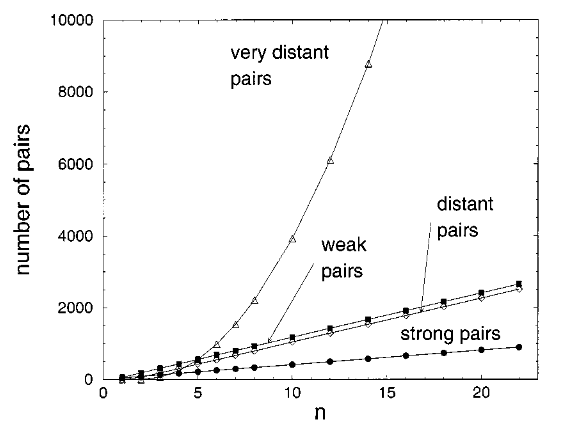
\includegraphics[scale=0.5]{Pics/electron_pairs.png}
\caption[Number of significant electron pairs in glycine chains.]{Number of significant electron pairs in glycine chains. Taken from \cite{Sch1999}}
\label{fig:EPAIRS}
\end{figure}

\subsubsection{Linear Scaling LMP2}

It has been found \cite{Sae1987} early on that the quadratic scaling very distant electron pairs can safely ignored without major impact on the total correlation energy. Distant pairs may also be approximated either by a multipole expansion \cite{Het1998} or empirically \cite{Rau1995}. As a consequence, this establishes a sparsity relationship between $i$ and $j$, and the sparsity diagram for the MO integrals becomes fully connected
\begin{center}
\begin{tikzpicture}

\snode{MU}{0,0}{\mu};
\snode{SIG}{1,0}{\sigma};
\snode{NU}{2,0}{\nu};
\snode{LAM}{3,0}{\lambda};

\snode{I}{0,-1}{\uli};
\snode{A}{1,-1}{\ola};
\snode{J}{2,-1}{\ulj};
\snode{B}{3,-1}{\olb};

\draw[<->] (MU) -- (SIG) node [midway, above] () {S};
\draw[<->] (NU) -- (LAM) node [midway, above] () {S};
\draw[<->] (I) -- (MU) node [midway, below] () {};
\draw[<->] (A) -- (SIG) node [midway, below] () {};
\draw[<->] (J) -- (NU) node [midway, below] () {};
\draw[<->] (B) -- (LAM) node [midway, below] () {};
\draw[<->] (I) -- (A) node [midway, below] () {};
\draw[<->] (J) -- (B) node [midway, below] () {};
\draw[<->] (I) |- (1,-1.5) node [below] {$1/R^6$} -| (J);

\end{tikzpicture}
\end{center}
\noindent Linear scaling MP2 can therefore be achieved with an LMO formulation \cite{Sch1999}.

% Sch1999 https://aip.scitation.org/doi/pdf/10.1063/1.479957
% distant pairs multipole approximate very distant pairs by multipole expansion Het1998 https://www.sciencedirect.com/science/article/pii/S0009261498004916
% distant pairs Empirically Rau1995 G. Rauhut, J. W. Boughton, and P. Pulay, J. Chem. Phys., 103, 5662 1995 .
%Instead of using distance criteria, can use screening: 
%https://aip.scitation.org/doi/10.1063/1.4773581
\subsubsection{Density Fitting for LMP2}

While specific virtual orbitals form a very compact representation of the virtual space, the fact that each electron pair has their own orthogonal virtual orbital basis means that the total number of virtuals can become exceedingly large, and consequently increases the cost associated with the AO-MO transformation step. The most expensive step then becomes
\begin{equation}
\cn{\uli\ola}{P} = L_{\mu\uli} \cn{\mu\nu}{P} L_{\nu\ola}
\end{equation}
\noindent Transformation of the 3c2e integrals scales with $\ccpx{2}$. Linear scaling can be achieved by introducing an orbital-specific fitting domain $[i]_{fit}$, e.g. by assigning all auxiliary functions $P$ on atoms with a Mulliken charge above a given threshold for the local orbital $i$ \cite{Pin2015}, or by using a Boughton-Pulay like scheme \cite{Wer2015}. This yields the sparsity diagram
\begin{center}
\begin{tikzpicture}

\snode{P}{-1,0}{P};
\snode{MU}{0,0}{\mu};
\snode{SIG}{1,0}{\sigma};

\snode{I}{0,-1}{\uli};
\snode{A}{1,-1}{\ola};

\draw[<->] (MU) -- (SIG) node [midway, above] () {S};
\draw[<->] (I) -- (MU) node [midway, below] () {};
\draw[<->] (A) -- (SIG) node [midway, below] () {};
\draw[<->] (I) -- (A) node [midway, below] () {};
\draw[<->] (I) -- (-1,-1) node [below] {LDF} -- (P);

\end{tikzpicture}
\end{center}
\noindent As opposed to SOS-AO-MP2, where density fitting can give a more favorable factorization of the energy expression, the MO integrals need to be fully assembled for LMP2 in order to solve the linear equations \ref{eq:MP2RES}. The assembly is done in two steps
\begin{align}
B^{X}_{\uli\ola} &= \sum_{Y \in [i]_{fit} \cup [j]_{fit}} \cn{X}{Y}^{-1/2} \cn{Y}{\uli\ola}
\\
\cn{\uli\ola}{\ulj\olb} &= \sum_{X \in [i]_{fit} \cup [j]_{fit}} B^{X}_{\uli\ola} B^{X}_{\ulj\olb} 
\end{align}
\noindent The two steps are repeated for each electron pair $ij$, and the sum runs over all auxiliary functions $P$ in the unified fitting domain $[i]_{fit} \cup [j]_{fit}$, which enforces linear scaling for these steps as well. 

% Pin2015 https://aip.scitation.org/doi/pdf/10.1063/1.4926879
% Wer2015 https://pubs.acs.org/doi/pdf/10.1021/ct500725e

\subsection{Natural Orbitals}

Pure natural orbital techniques are generally not used in the context of MP2, given that MP2 is also used as a guess density to obtain the natural orbitals. Rather, NOs are more popular in the context of coupled cluster methods like CCSD and CCSD(T), though there have been some application in the context of PNOs \cite{Fra2017,Sch2013} and domain-based local PNOs (DLPNO) \cite{Wer2015,Pin2018}. The latter combines the compact virtual representation of PNOs with the local electron-pair treatment of LMOs   described in the previous sections. 

As was previously explained, the main idea of NOs is to truncate the virtual space by omitting all orbitals with an occupation number below a certain threshold. The MO integrals in the truncated NO basis can then be plugged into one of the orbital-invariant formulations of the MP2 energy expressions, or they can be canonicalized to be used in the standard MP2 expressions.

\section{Coupled Cluster}

Virtually all of the concepts introduced in the previous section can also be applied in the context of coupled cluster. Local MP2 and local CC evaluate the MO integrals in the same exact manner, either using LMOs \cite{Sch2001, Sch2002, Sch2000a, Sch2000b,Sch2001}, natural orbitals \cite{Tau2008,Nag2018,Rol2013} or pair-natural orbitals \cite{Nee2009a,Guo2018,Sch2017,Rip2013}. The orbital-invariant CC amplitude equations can then be directly solved at a reduced cost by plugging in the truncated MO integrals.

An atomic orbital formulation of the coupled cluster equations is possible \cite{Scu1999}, but has never been pursued further. Again, the AO-CCSD method as presented by Scuseria et al. is not really a pure AO-method, but rather a PAO-like approach similar to PAO-CCSD later proposed by Christiansen and Koch \cite{Chr2006}. The reason why AO/PAO coupled cluster methods have not been popular is likely due to the very high prefactor for larger basis sets, which are often crucial for obtaining accurate correlation energies. Moreover, in contrast to MP$n$ amplitudes, the coupled cluster amplitudes do not have closed expressions, which in turn inhibits any further factorizations of coefficient matrices to reduce the overhead like in Cholesky decomposed MP2, with the exception of hybrid methods like CC2 \cite{Sac2021}.

%AO: Scu1999
%LNO: Nag2018 (CCSD(T)) Rol2013 (CCSD(T), 
%PNO: Nee2009, Guo2018 (CCSD(T) DPLNO), LPNO CCSD(T) Sch2017, Rip2013 CCSD, 
%LMO: Sch2001 (CCSD), Sch2002 (CCSDT) Sch2000, Sch2000a (CCSD(T)) , 
%FNO Bar2005

%\subsection{Atomic Orbital CC2}
%
%The atomic orbital approach for low scaling MP2 can be extended to CC2 ... currently under work
%
%\subsection{Atomic Orbital CCSD: PAO or AO?}
%
%!!!!!!!!!!!!! REWRITE !!!!!!!!!!!!!!!!
%As opposed to MP2 and CC2, where the energy denominator in the closed form expression for the doubles amplitudes $t_{iajb}$ makes it difficult to find an orbital-invariant representation of the energy expressions, it is much easier to do so for CCSD. The restricted CCSD correlation energy expression reads
%\begin{equation}
%E_{corr} = \sum_{ijab} v_{iajb} t^{CCSD}_{iajb} \qquad v_{iajb} = 2\cn{ia}{jb} - \cn{ib}{ja} 
%\end{equation}   
%\noindent In their 1999 paper [ref], Scuseria and Ayala have shown that there are two possible "AO" representations of the CCSD correlation energy. The first and most straight-forward approach is to factor out the MO coefficient matrices from the MO electron repulsion integrals $v$, similar to AO-MP2
%\begin{equation}
%\begin{split}
%E_{corr} &= \sum_{ijab} \sum_{\mu\nu\sigma\lambda} C_{\mu i} C_{\sigma  a} v_{\mu\sigma\nu\lambda} C_{\nu j} C_{\lambda b} t_{iajb} \\
%&= \sum_{\mu\nu\sigma\lambda} v_{\mu\sigma\nu\lambda} t_{\ulgm\olgs\ulgn\olgl}
%\end{split} 
%\end{equation}
%\noindent whith the amplitudes $\mathbf{t}$ recast in a PAO-like basis:
%\begin{equation}
%t_{\ulgm\olgs\ulgn\olgl} = C_{\mu i} C_{\sigma a} t_{iajb} C_{\nu j} C_{\lambda b}
%\end{equation}
%\noindent The MO amplitudes can be recovered with
%\begin{equation}
%t_{iajb} = \ovl{C}_{\mu i} \ovl{C}_{\sigma a} t_{\ulgm\olgs\ulgn\olgl} \ovl{C}_{\nu j} \ovl{C}_{\lambda b}
%\end{equation}
%\noindent It should be noted that $\ulgm$, $\olgs$, $\ulgn$ and $\olgl$ do not correspond to the definition of PAOs given in Section .... As opposed to standard PAOs, they lack the overlap matrix $\mathbf{S}$ in the MO-PAO transformation and vice-versa (compare Equation ... with Eqaution ...). Here, the occupied and virtual PAO-like spaces are not mutually orthogonal, but related through the overlap matrix, similar to the pseudo-PAOs used in AO-MP2
%\begin{equation}
%\mathbf{PSQ} = \mathbf{0} \qquad \mbf{P} + \mbf{Q} = \mbf{S}^{-1}
%\end{equation}
%\noindent This alternative PAO-like formulation will be referred to as \emph{mutually non-orthogonal projected atomic orbitals} (or mnoPAOs) from here on out.    
%
%\noindent Instead of using this mnoPAO approach, Scuseria and Ayala proposed an alternative formulation where the coefficient matrices are factored out from the t-amplitudes instead, using the PAO backtransformation \ref{CMO2PAO}:
%\begin{equation}
%\begin{split}
%E_{corr} &= \sum_{ijab} \sum_{\mu\nu\sigma\lambda} v_{iajb} C_{\mu i} C_{\sigma  a} \theta_{\ulgm\olgs\ulgn\olgl} C_{\nu j} C_{\lambda b} \\
%&= \sum_{\mu\nu\sigma\lambda} \Pi_{\ulgm\olgs\ulgn\olgl} \theta_{\ulgm\olgs\ulgn\olgl}
%\end{split} 
%\end{equation}
%\noindent The PAO-amplitudes $\theta$ are related to the MO quantities by
%\begin{equation}
%\theta_{\ulgm\olgs\ulgn\olgl} = \ovl{C}_{\mu i} \ovl{C}_{\sigma a} t_{iajb} \ovl{C}_{\nu j} \ovl{C}_{\lambda b}
%\end{equation}
%\begin{equation}
%t_{iajb} = C_{\mu i} C_{\sigma a} \theta_{\ulgm\olgs\ulgn\olgl} C_{\nu j} C_{\lambda b}
%\end{equation}
%\noindent The mnoPAO and PAO t-amplitudes are related by
%\begin{equation}
%\theta_{\ulgm\olgs\ulgn\olgl} = S_{\mu\mu'} S_{\olgs\olgs'} t_{\ulgm'\olgs'\ulgn'\olgl'} S_{\ulgn\ulgn'} S_{\olgl\olgl'}  
%\end{equation}
%\begin{equation}
%\theta_{\ulgm\olgs\ulgn\olgl} = P_{\mu\mu'} P_{\olgs\olgs'} \theta_{\ulgm\olgs\ulgn\olgl} P_{\ulgn\ulgn'} P_{\olgl\olgl'} 
%\end{equation}
%!!!!! REWRITE !!!!!!!!!!!
%
%\subsection{Local Coupled Cluster}
%
%\subsection{FNO Coupled Cluster ??}
%
%\section{Critical Stance on AO vs LMO} 
%
%Distance criteria, or Mulliken/Löwdin pouplation
%AO only for closed expressions (not for CCSD++) 
%LOcal: ij cirteria, ij->ab criteria % https://www.sciencedirect.com/science/article/pii/S1574140006020044?via%3Dihub
%
%% Hylleraas functional: 
%% Hyl1930 https://link.springer.com/article/10.1007/BF01397032
%
%% First use of LMO+PNOs with Hylleraas 
%% Pul1986 https://link.springer.com/article/10.1007%2FBF00526697
%
%% LInear scaling of the functional
%% Linear scaling of electron inetgrals
%% linear scaling of MO-AO transformation -> or density fitting

%\section{Summary}
%
%LMO vs PNO vs NO ?

\chapter{Local Correlation Methods (III): Excited States}

While local correlation methods for the ground state have been around since the 1980s, the extension of the local treatment of electron correlation to excited states is relatively new. With the earliest attempts dating back to the 2000s, many new approaches and approximations have emerged over the last decade, building on the concepts of LMOs, NOs and PNOs. One of the major obstacles that makes a straight-forward extension to excited states difficult is the long-range character of certain excitations, such as charge transfer states. In contrast to the description of electron correlation in the ground state, the occupied and virtual orbitals involved in electron transitions can be very far apart. This means that the optimal molecular orbital space for the excited state can be very different from that of the ground state. 

This chapter presents the state of the art for local correlated excited state methods (ADC, CCLR, EOM-CC) for LMOs, NOs, PNOs, and combinations thereof. Atomic orbital approaches are discussed as well. 

% Bau2017 CornFlex https://aip.scitation.org/doi/pdf/10.1063/1.4984820

% Linear‐scaling self‐consistent field methods for large molecules
% https://aip.scitation.org/doi/pdf/10.1063/1.2961039

\section{Low-Scaling Correlated Excited State Methods}

All of the existing low-scaling implementations of ADC, CCLR and EOM use some form of local or compact molecular orbital representation, to varying degrees of success. As mentioned above, the major problem that these methods face is the non-locality of certain excited states such as charge transfer states, which can involve occupied and virtual orbitals which are localized on entirely different parts in the system. Clearly, truncating virtual orbitals spatially is no longer a valid option, and makes a straight-forward extension of LMO-methods difficult, because they cut out far-away contributions. Similar problems are encountered in NO formulations, as the excited state is often not properly described by the electronic ground state (pair-)densities and their associated (pair) natural representation. Over the years, various strategies have been proposed to adapt existing LMO and NO schemes to excited states as well. 

\subsection{Orbital Invariance of the Matrix Expressions}

Correlated excited state methods involve some form of symmetric or non-symmetric eigenvalue problem, which is generally solved using the Davidson procedure. The time-determining step is given by the computation of the matrix-vector product of the ADC, CC response, or EOM-CC matrix $\mbf{A}$ with the Davidson trial vectors $\mbf{u}$
\begin{equation}
\mbf{r} = \mbf{A} \mbf{u}
\end{equation}
\noindent Closed expressions can be derived for the MVPs, with the matrix elements computed on the fly. The MVPs and trial vectors are divided into blocks of singles, doubles, triples, ... ($u_i^a$, $u_{ij}^{ab}$, $u_{ijk}^{abc}$) depending on the level of approximation of the underlying methods. In the case of ADC(2), the MVP is split according to
\begin{align}
r_{ia} &= A_{ia,jb} u_{jb} + A_{ia,jbkc} u_{jbkc} \\
r_{iajb} &= A_{iajb,kc} u_{kc} + A_{iajb,kcld} u_{kcld} 
\end{align}
\noindent The eigenvalue problem is generally solved in the canonical molecular orbital basis, but other orbital representations can also be used, by swapping all the CMO quantities $\cn{ia}{jb}$, $t_{iajb}$, ... by their local counterparts $\cn{\uli\ola}{\ulj\olb}$, $t_{\uli\ola\ulj\olb}, ...$. The eigenvalue problem can then be solved e.g. in an LMO basis, or the MVPs can be computed in the LMO basis and transformed to the CMO basis using the transformation matrix $\mbf{U}$:
\begin{equation}
r_{ia} = U_{i\uli} r_{\uli\ola} U_{\ola a} 
\end{equation}
\noindent The eigenvalues of the LMO matrix appear to not differ from the ones obtained via a CMO formalism \cite{Kat2009}.

For local EOM-CC and CCLR, the singles and doubles amplitudes $t_{\mu_1}$ and $t_{\mu_2}$ are determined iteratively from a local ground state calculations using the techniques in the previous chapter for reduced scaling. For the approximate EOM-CC2 and CC2-LR methods, as well as ADC(2), the MP2 amplitudes may also be computed iteratively in the local basis using the Hylleraas functional, or using a closed form expression via the Laplace transform techniques.   

EOM-CC2, CC2-LR and ADC(2) allow for an on-the-fly computation of the doubles part (see section \ref{sec:ADC_DAV}). Here, the orbital invariant formulation becomes less straight-forward because the doubles-doubles block of the non-canonical ADC and CC2 Jacobian matrix is not diagonal. Fortunately, the Laplace transform can be applied to circumvent this problem. Using the ADC(2) eigenvalue problem as an example, the doubles-folded MVP expression is given by
\begin{equation}
\begin{split}
r_{ia}(\omega) &= A_{ia,jb} u_{jb} + A_{ia,jbkc} \frac{A_{iajb,kc} u_{kc}}{\omega - \eps_a - \eps_b + \eps_i + \eps_j} \\
&= A_{ia,jb} u_{jb} - \sum_{\alpha}^{n} |w\pa| e^{\left(\omega - \eps_a - \eps_b + \eps_i + \eps_j\right) t\pa} A_{ia,jbkc} A_{,kc} u_{kc} 
\end{split}
\end{equation}
After transforming to the LMO basis, the local ADC(2) equations read
\begin{equation}
r_{\uli \ola}(\omega) = A_{\uli \ola, \ulj \olb} u_{\ulj \olb} - A_{\uli \ola, \ulj \olb \ulk \olc} \sum_{\alpha}^{n} e^{\omega t\pa} X_{\ulj \ulj'}\pa Y_{\olb \olb'}\pa A_{\ulj' \olb' \ulk' \olc', \ull \old} u_{\ull \old} X_{\ulk \ulk'}\pa Y_{\olc \olc'}\pa  \\
\end{equation}
\noindent with the Laplace matrices $\mathbf{X}$ and $\mathbf{Y}$ 
\begin{equation}
X_{\uli\ulk}\pa = \sum_i U_{i\uli} |w^{'(\alpha)}|^{1/4} e^{\eps_i t^{'(\alpha)}} U_{k\ulk}
\end{equation}
\begin{equation}
Y_{\ola\olc}\pa = \sum_a U_{a\ola} |w^{'(\alpha)}|^{1/4} e^{-\eps_a t^{'(\alpha)}} U_{c\olc}
\end{equation}
\noindent Note that the optimal Laplace parameters $w^{'(\alpha)}$ and $t^{'(\alpha)}$ are different from the ones used in the MP2 amplitudes, due to the presence of the eigenvalue $\omega$ in the denominator. Each time the eigenvalue changes, the Laplace parameters need to be recomputed to obtain an accurate approximation. 

An orbital invariant reformulation is not needed by every method. NOs, PNOs and NTOs can be \emph{canonicalized} by diagonalizing the occupied-occupied and virtual-virtual block of the Fock matrix in the truncated NO/PNO/NTO basis to get a smaller set of canonical molecular orbitals and orbital energies. Because these types of representations generally do not depend on distance criteria, they are unaffected by the delocalized nature of the canonical basis, as they seek compactness rather than locality. 

\subsection{Local Molecular Orbitals and Domains}

The most challenging part in extending domain-specific virtual orbital methods to excited states lies in determining a suitable excitation domain in which to expand the virtual space. The first implementations of local excited state EOM-CCSD \cite{Cra2002,Kor2003} and CC2-LR \cite{Kat2006} constructed the domains using a Mulliken-charge like analysis of the CIS coefficients $r_{ia}$. The CIS coefficients are first transformed to the LMO-PAO basis
\begin{equation}
r_{\uli \olgm} = U_{\uli i } r_{ia} \bar{C}_{\mu a} 
\end{equation}
\noindent To determine the importance $w$ of each LMO/PAO, the squares of the norms of the coefficients are summed up row- and column-wise
\begin{equation}
\begin{split}
w_{\uli} &= \sum_{\mu} |r_{\uli \olgm}|^2 \\
w_{\olgm} &= \sum_{\uli} |r_{\uli \olgm}|^2
\end{split}
\end{equation}
\noindent The LMOs/PAOs are then ordered by decreasing weight. Their weights are then summed up until a certain threshold $T_{LMO}$/$T_{PAO}$ is reached (typically around 0.995 to 0.9999). The excited state orbital domains $[\uli]_{ES}$ containing the relevant virtual orbitals are then constructed by applying the Boughton-Pulay algorithm to a set of "excited natural orbitals" \cite{Kor2003}
\begin{equation}
\phi_{\uli}^* = \sum_{\ola} r_{\uli \olgm} \phi_{\olgm}  
\end{equation} 
\noindent The full orbital domain of $i$ is then given as the union of its ground-state and excited state domain $[\uli]$ = $[i]_{GS} \cup [i]_{ES}$. The virtual orbital weights $w_{\olgm}$ can be used to impose further restrictions on the virtual orbital space. Finally, the pair domains $ij$ are formed as the union $[\uli] \cup [\ulj]$. In general, only the computation of the doubles part, which is time-determining, is subject to domain-restrictions, while the singles part is computed without domain lists.

The method however has the major flaw that the orbital domains are highly sensitive to the CIS transition density, which does not describe the excited state very accurately. Some orbitals can be dropped in the domain construction which might become important for doubles contributions. LMO methods face an interesting chicken-or-egg problem where they need information from the excited state wave function, to accurately compute properties of said function. There are several ways to address this problem. In their local CC2-LR implementation, Kats and Schütz \cite{Kat2009} use Laplace transformed doubles folding to recompute the doubles amplitudes on the fly, which allows to adapt the excited state domains dynamically during the optimization procedure. Starting from the CIS transition density, the domains are recomputed at each step by analyzing the state vector $r_{\uli \olgm}(\omega)$ as described above. This greatly increased accuracy compared to canonical calculations with energy differences well below 0.1 eV.

Mester et al. \cite{Mes2017} proposed a more pragmatic approach, where they first analyze the CIS state vector to extract the important LMOs and PAOs. They then augment the domains $[i]_{EX}$ by adding all remaining molecular orbitals that have a significant Mulliken charge on an atom that is also significant for $i$. This is based on the assumption that, although CIS might not be a good approximation, the important orbitals should still be close by. 

Nonetheless, the LMO method is again plagued by spurious distance dependent thresholds and Mulliken charge thresholds. Nowadays, low scaling excited state methods are mostly dominated by PNOs, NOs, or NTOs.

% Kor2003 First EOM-CCSD Korona, T.; Werner, H.-J. Local treatment of electronexcitations in the EOM-CCSD method.J. Chem. Phys.2003,118,3006.
% Also first EOM-CCSD Cra2002 Crawford, T. D.; King, R. A. Locally correlated equation-of-motion coupled cluster theory for the excited states of largemolecules.Chem. Phys. Lett.2002,366, 611.
% https://aip.scitation.org/doi/10.1063/1.3237134

\subsection{Natural Orbitals}

NO methods achieve performance by dropping virtual natural orbitals with low occupation numbers. The first implementations of EOM-CC and CCLR in the NO representation used natural orbitals obtained from the diagonalization of the ground state MP2 density matrix \cite{Lan2010}. A reasonable speed-up could be observed, although the excited state character was not taken into account. However, it was shown \cite{Kum2017} that properties like the polarizability are much more sensitive to the truncation of the virtual orbitals than the ground state correlation energy, with the error increasing linearly as a function of the number of dropped virtual natural orbitals. While VNOs with low occupation numbers, i.e. diffuse character, can be safely  ignored for the ground state correlation energy, diffuse VNOs play a much more important role for response properties, and hence fewer VNOs can be omitted. Better results could be obtained by simply truncating the virtual CMOs instead, which invalidates the use of VNOs. 

In their NO-CC2 and NO-ADC(2) implementations, Mester et al. \cite{Mes2017, Mes2018, Mes2019} proposed to compute a set of occupied and virtual NOs by diagonalizing the occupied and virtual state-averaged densities
\begin{equation}
\mathbf{D}_{ij} = \frac{1}{2} \left( \mathbf{D}_{ij}^{MP2} + \mathbf{D}_{ij}^{CIS(D)} \right)
\end{equation}
\begin{equation}
\mathbf{D}_{ab} = \frac{1}{2} \left( \mathbf{D}_{ab}^{MP2} + \mathbf{D}_{ab}^{CIS(D)} \right)
\end{equation}
\noindent where $\mathbf{D}^{MP2}$ is the MP2 ground state density and $\mathbf{D}^{CIS(D)}$ is the state-specific CIS(D) excited state density. Their restricted expressions read
\begin{equation}
D_{ij}^{MP2} = \sum_{kab} \left( 2 t_{ik}^{ab} t_{jk}^{ab} - t_{ik}^{ab} t_{jk}^{ab} \right) 
\end{equation}
\begin{equation}
D_{ab}^{MP2} = \sum_{ijc} \left( 2t_{ij}^{ca} t_{ij}^{cb} - t_{ij}^{ca}t_{ij}^{bc} \right)
\end{equation}
\begin{equation}
D_{ij}^{CIS(D)} = \sum_{a} c_i^a c_j^a  + \sum_{kab} \left( 2 t_{ik}^{ab} t_{jk}^{ab} - t_{ik}^{ab} t_{jk}^{ab} \right) 
\end{equation}
\begin{equation}
D_{ab}^{CIS(D)} = \sum_{i} c_i^a c_i^b + \sum_{ijc} \left( 2c_{ij}^{ca} c_{ij}^{cb} - c_{ij}^{ca}c_{ij}^{bc} \right)
\end{equation}
\noindent where $c_i^a$ are the CIS coefficients and the $c_{ij}^{ab}$ are the CIS(D) doubles coefficients
\begin{equation}
c_{ij}^{ab} = \frac{\sum_c \left[ \cn{ac}{bj} c_i^c + \cn{ac}{bi} c_j^c \right] - \sum_k \left[ \cn{kj}{ai} c_k^b + \cn{kj}{bj} c_k^a \right]}{D_{ij}^{ab} + \omega_{CIS}}
\end{equation}
\noindent The state-averaged density needs to be recomputed and diagonalized for each state because $\mathbf{D}^{CIS(D)}$ depends on the excitation energy $\omega$. While the CIS(D) density is much easier to compute than the ADC(2) or CC2-LR state density, it still scales with $\ccpx{5}$. To reduce the computational complexity, the density is constructed in a truncated orbital space: first, a set of occupied and virtual LMOs are chosen according to the CIS weighting criteria $w$ described in the previous section. The basis is augmented by spatially close orbitals, and then canonicalized to yield a highly compact orbital molecular space which lowers the cost of constructing the CIS(D) densities. 

In combination with natural auxiliary functions, this hybrid NO-LMO scheme can reduce the timings for CC2 and ADC(2) to such a drastic extent that the CIS pre-iterations become the time-determining step (Figure \ref{fig:MESTER}), with an additional error of only 2-4 meV. The reduced scaling however comes at a high prefactor when computing multiple different excitation energies. 

\begin{figure}
\centering
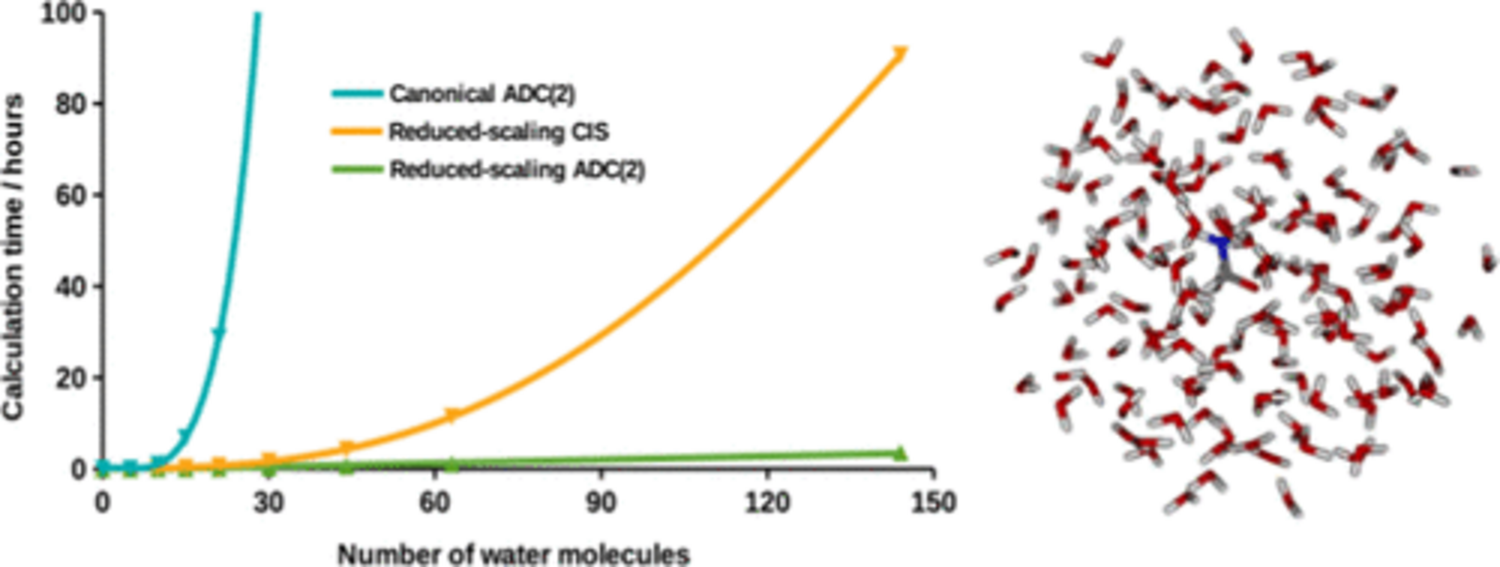
\includegraphics[scale=1.0]{Pics/mester_adc.png}
\caption[Wall times of CIS compared to NO-ADC(2) as a function of system size of hydrated formamide.]{Wall times of CIS compared to NO-ADC(2) as a function of system size of hydrated formamide. Taken from \cite{Mes2019}.}
\label{fig:MESTER}
\end{figure}

% Reduced NO CC2 Mes2017 https://aip.scitation.org/doi/10.1063/1.4983277
% EOM NO Lan2010 https://aip.scitation.org/doi/10.1063/1.3276630
% CCLR NO Kum2017 https://pubs.acs.org/doi/10.1021/acs.jpca.6b11410
% Reduced ADC(2) Mes2018 https://aip.scitation.org/doi/10.1063/1.5021832
% Reduced ADC(2) Mes2019  https://pubs.acs.org/doi/pdf/10.1021/acs.jctc.9b00735
% CIS(D) Hea1994 https://www.sciencedirect.com/science/article/pii/0009261494000700?via%3Dihub

\subsection{Pair Natural Orbitals}

Pair natural orbital methods face the same problems as NOs, where PNOs with low occupation numbers are considerably more important for response properties than for ground state properties \cite{McA2016}. In a similar vein, excited state PNOs can be generated by considering lower level excited state electron pair densities \cite{Hel2011}. PNO methods have been successfully extended to ADC(2), CC2-LR \cite{Hel2013}, ADC(2)-x \cite{Hel2014} and CCSD-LR \cite{Fra2018} by using CIS(D) or CIS(D)-like densities
\begin{equation}
D_{ij}^{ab} = \sum_c \left( 2b_{ij}^{ab} - b_{ij}^{ba} \right) b_{ij}^{ab} + \left( 2b_{ij}^{ab} - b_{ij}^{ba} \right) b_{ij}^{ba}
\end{equation}
\noindent where $\mathbf{b}_{ij}$ are state-specific modified pair amplitudes which are not uniquely defined. Again, these methods come at the cost of a higher prefactor due to the relatively high cost of constructing PNOs. %Nonetheless, it was shown that the computational complexity can be lowered to $\ccpx{3}$ for PNO-CCSD-LR. 

Efforts have also been made to develop PNO response methods which are more economical for computing larger excitation manifolds by removing the state-specificity. Instead of taking individual excited state densities, Peng et al. \cite{Pen2018} proposed to generate a set of \emph{state-averaged} PNOs obtained by diagonalization of the average excited state density over an $N$-state manifold 
\begin{equation}
\mathbf{D}_{ij} = \frac{1}{N} \sum_k^N \mathbf{D}_{ij}^{(k)}
\end{equation}
\noindent A production-quality implementation has not yet been shown which uses this approach.

In their perturbed pair-natural orbital (PNO++) approach for CCLR, Cunha and Crawford \cite{DCu2021} incorporate the external perturbation into the electron pair density
\begin{equation}
D_{ij}^{ab} = \sum_c \left( 2x_{ij}^{ab} - x_{ij}^{ba} \right) x_{ij}^{ab} + \left( 2x_{ij}^{ab} - x_{ij}^{ba} \right) x_{ij}^{ba}
\end{equation}
\noindent where $\mathbf{x}$ are perturbed amplitudes given by
\begin{equation}
x_{ij}^{ab} = \frac{\overline{B}}{\ovl{H}_{aa} + \ovl{H}_{bb} - \ovl{H}_{ii} - \ovl{H}_{jj} + \omega}
\end{equation}
\noindent with an external perturbation $\ovl{B}$ and the similarity transformed Hamiltonian $\ovl{H}$. This gives a set of "perturbation-aware" PNOs customized for a given external perturbation \cite{Cra2019}. 

Finally, there are also the \emph{back-transformed} PNOs, or bt-PNOs, where the ground state PNO-quantities like the amplitudes are transformed back to the canonical basis and used in the canonical working equations \cite{Dut2016}.

In the end, most local excited state methods using natural orbitals differ by how they redefine the amplitudes $\mathbf{b}$ for the individual excited states or the whole perturbed molecular system. It is still an active field of research.

% PNO-CIS(D) Hel2011 https://aip.scitation.org/doi/10.1063/1.3664902 [Uses CIS(D) pair density]
% PNO-CC2 Hel2013 https://aip.scitation.org/doi/10.1063/1.4819071 [Uses Excited state OSVs to construct PNOs] 
% PNO-ADC(2)-x: Hel2014 https://www.sciencedirect.com/science/article/pii/S2210271X14001194?via%3Dihub [Also use excited state specific desnity to get OSVs using modified CIS(D) like desnities CC2/ADC(2)-x densities Dii_ab
% PNO-CCSD https://aip.scitation.org/doi/full/10.1063/1.5018514 [Also CIS(D) like density] 

% PNOs have similar Problem than NOs: Har2016  https://pubs.acs.org/doi/10.1021/acs.jctc.5b00898
% Because diffuseness. Solution: Cra2019 PNO++ https://onlinelibrary.wiley.com/doi/10.1002/wcms.1406
% PNO++-CCSD-LR Cun2021 https://pubs.acs.org/doi/pdf/10.1021/acs.jctc.0c01086

% State-averaged Pen2018 https://arxiv.org/pdf/1802.06738.pdf
% bt-PNOs Dut2016 https://aip.scitation.org/doi/pdf/10.1063/1.4958734
 
\subsection{Natural Transition Orbitals}

The last method to obtain a compact representation of excited states is via natural transition orbitals. NTOs are the equivalent of NOs for excited states, and represent a compact representations of their dominant contribution (Figure \ref{fig:NTO}). Baudin and Kristensen have developed two different CC2-LR schemes based on NTOs called LoFEX (local framework for calculating excitation energies) \cite{Bau2016} and CornFLEX (correlated natural transition orbital framework for calculating excitation energies) \cite{Bau2017} 

Again, one needs information about the excited state to efficiently compute its properties. The LoFEX method starts with a time-dependent Hartree Fock calculation and generates a set of NTOs by decomposition of the TDHF transition vectors $\mathbf{r}$ by diagonalization
\begin{align}
\mathbf{r} \mathbf{r}^{\dagger} \mathbf{U} &= \lambda_o \mathbf{U} \\
\mathbf{r}^{\dagger} \mathbf{r} \mathbf{V} &= \lambda_v \mathbf{V}
\end{align}
\noindent which is just an alternative way to compute the occupied and virtual NTO transformation matrices $\mathbf{U}$ and $\mathbf{V}$, rather than by singular value decomposition. A set of dominant NTO pairs is then chosen for which their occupation numbers are above a given threshold $\tau_{LoFEX}$. The non-dominant NTOs are not discarded, but rather localized. The idea is to construct a surrounding excitation orbital space (XOS) containing LMOs that are important for correlation effects of the NTOs. A first guess to the XOS is chosen based on distance criteria and Löwdin charges. The CC2-LR eigenvalue problem is then solved in that basis, and new NTOs are computed from the CC2 transition vector and added to the XOS. This procedure is repeated until the excitation energy $\omega$ for that state has converged. While the guess XOS is first formed using distance criteria, the subsequent optimization procedure makes the method much more robust and black-box. Even for relatively small molecules, LoFEX can obtain considerable speed-ups. The main disadvantage is that LoFEX does not give any leverage for very delocalized excitations. 

The improved CornFLEX method constructs a set of CIS(D)-like NTOs (CIS(D')-NTOs) which is obtained from diagonalizing a CIS(D)-like density matrix in the CIS-NTO basis. As opposed to CIS-NTOs, the CIS(D') NTOs also include correlation effects and are a more robust representation that the simple ad-hoc extension of CIS-NTOs using LMOs. Speed-ups can be observed in CornFLEX even for delocalized excitations.

% Bau2016 https://aip.scitation.org/doi/pdf/10.1063/1.4953360
% Bau2017 https://aip.scitation.org/doi/pdf/10.1063/1.4984820

\begin{figure}
\centering
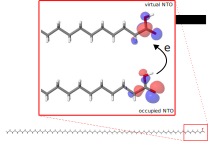
\includegraphics[scale=0.6]{Pics/NTOACID}
\caption[Dominant natural transition orbital pair for the lowest excitation of the carboxylic acid C$_{79}$H$_{159}$COOH.]{Dominant natural transition orbital pair for the lowest excitation of the carboxylic acid C$_{79}$H$_{159}$COOH ($\pi \rightarrow \pi^*$ transition). The span of the NTOs is very small compared to the rest of the molecule, and the compactness can be used to drastically speed up excited state calculations.}
\label{fig:NTO}
\end{figure}

\section{Atomic Orbital Configuration Interaction Singles}

%-> AO TDSCF (Kussmann)
%-> TDHF and RPA are equivalent in linear response regime. % see https://www.frontiersin.org/articles/10.3389/fphy.2019.00020/full

The methods presented in the previous section all work similarly. They first start by approximating the targeted excited states with a lower level of theory using CIS or CIS(D). They then solve higher order equations in the basis obtained from that approximation and may also dynamically augment the correlation domain while optimizing the excitation energies. The methods work on the principle of orbital \emph{compactness} rather than sparsity

At the moment of writing, CIS is the only excited state method which is routinely evaluated using an AO approach. While CIS does not give qualitatively good results, it is still a very important stepping stone for higher order methods, as was demonstrated in the previous section. Omitting the zero-order contributions, the CIS working equations are given by
\begin{equation}
r_{ia} = \left[ 2 \cn{ia}{jb} - \cn{ib}{ja} \right] u_{jb}
\end{equation}
\noindent Factoring out the MO coefficient matrices:
\begin{equation}
\begin{split}
r_{ia} &= C_{\mu i} C_{\sigma a} \left[ 2 \cn{\mu\sigma}{\nu\lambda} - \cn{\mu\lambda}{\nu\sigma} \right] C_{\nu j} C_{\lambda b} u_{jb} \\ 
&= C_{\mu i} C_{\sigma a} \left[ 2 \cn{\mu\sigma}{\nu\lambda} - \cn{\mu\lambda}{\nu\sigma} \right] P_{\nu\lambda} 
\end{split}
\end{equation} 
\noindent where $\mathbf{P}$ is the non-symmetric transition density in the AO basis. The CIS working equations can be reduced to the construction of a "pseudo"-Fock matrix which has a Coulomb and an exchange part. The Fock matrix is then transformed to the MO basis:
\begin{align}
F_{\mu\nu} &= J_{\mu\nu} + K_{\mu\nu}  \\ 
r_{ia} &= C_{\mu i} F_{\mu\nu} C_{\mu a}  
\end{align}
\noindent For localized excitations, the AO transition density is sparse (Figure \ref{fig:CISDENSE}), and similar approximation can be used as in Hartree Fock, e.g. LinK, CFMM, or LDF. CIS can therefore be evaluated with $\mathcal{O}(N)$ computational effort. Strictly speaking, it is not a "pure" AO formulation, because the AO intermediates still need to be transformed to the MO basis.

\begin{figure}
\centering
\begin{subfigure}{0.3\linewidth}
\centering
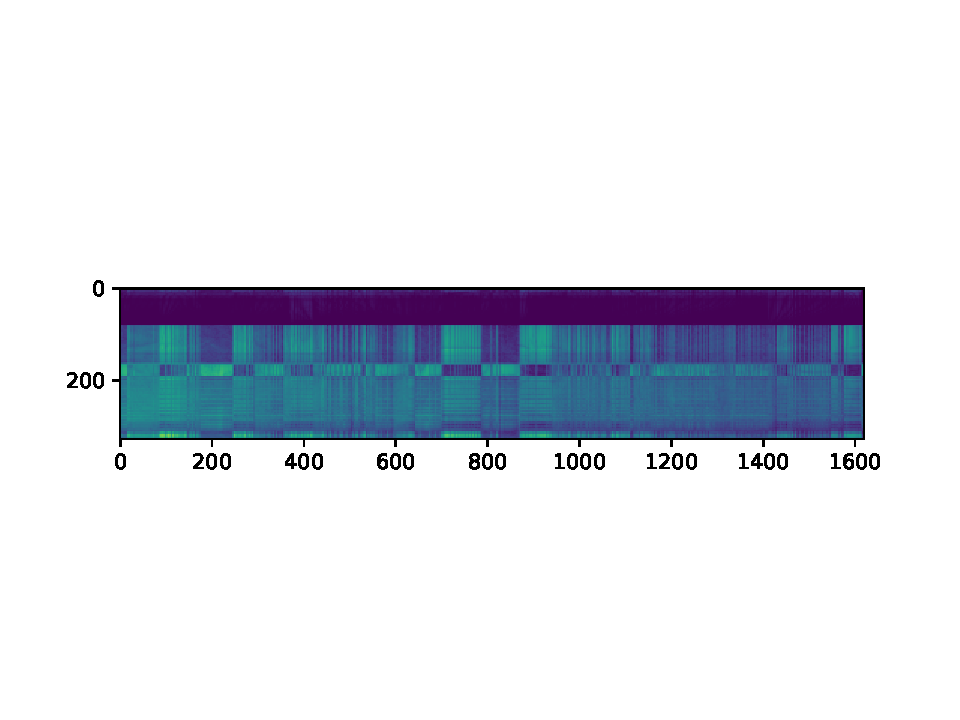
\includegraphics[scale=0.6]{Pics/CISDENSE}
\caption{}
\end{subfigure}
$\Longrightarrow$
\begin{subfigure}{0.6\linewidth}
\centering
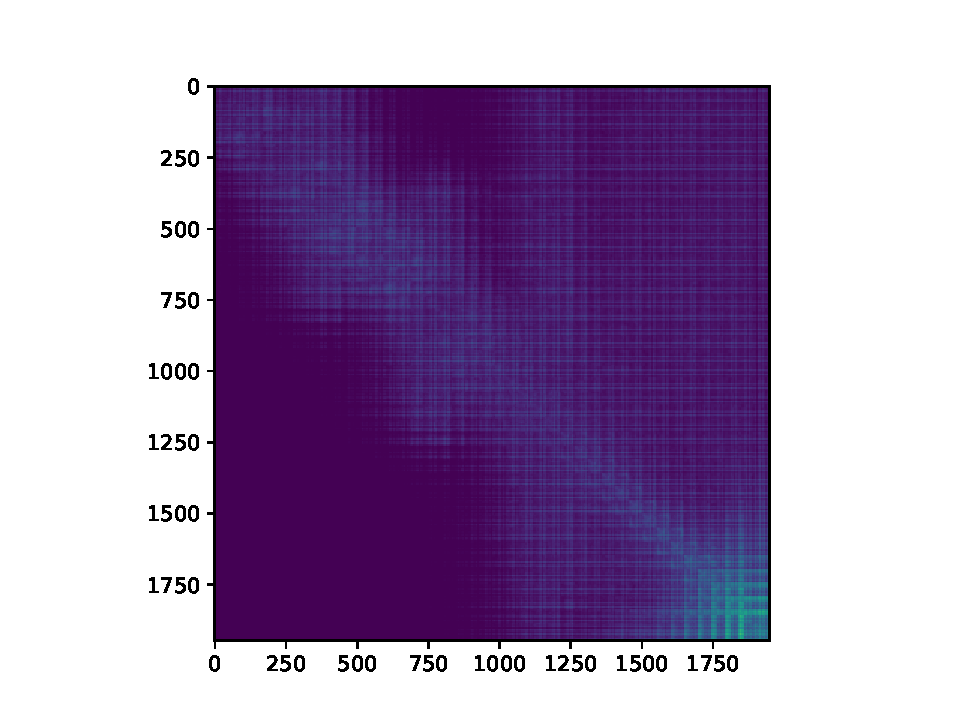
\includegraphics[scale=0.6]{Pics/CIS}
\caption{}
\end{subfigure}
\caption[Logarithm of the absolute values of the matrix elements in the transition densities in the MO and AO basis for the lowest excited state for the carboxylic acid C$_{79}$H$_{159}$COOH.]{Logarithm of the absolute values of the matrix elements in the transition densities in the MO (left) and AO basis (right) for the lowest excited state for the carboxylic acid C$_{79}$H$_{159}$COOH. The excitation domain is entirely localized on the carboxylic group. Using sparse matrix algebra, significant speed-ups can be obtained for CIS in the AO basis.}
\label{fig:CISDENSE}
\end{figure}

% PAO CCLR not good! Look at Gunnar review article perhaps

% First appearance of local EOM-CCSD 
% Cra2002 https://aip.scitation.org/doi/pdf/10.1063/1.1537718

% First appearance of local CCLR CC2 (no doubles wrapping) Kat2006 https://aip.scitation.org/doi/pdf/10.1063/1.2339021
% Flaw: Domains dtermined from CCS, bad if not correponding to good approximat. ALso fixed during davidson

% Kat2009 https://aip.scitation.org/doi/pdf/10.1063/1.3237134
% FIxes Problem by refreshing domains

% state-specific PNOs from CIS(D) Hel2011 https://aip.scitation.org/doi/10.1063/1.3664902

% Hel2013 PNO-CC2 https://aip.scitation.org/doi/10.1063/1.4819071

% Hel2014 PNO-ADC2 https://www.sciencedirect.com/science/article/pii/S2210271X14001194?via%3Dihub

%PURE AO FORMULATION THOULESS INTEGRAL
%PROBLEM: MO ENERGIES ARE NEEDED. if a pure ao algorithm, most likely a whole other approach that tries to get "density metrix perturbation"

\section{Molecular Orbital-free Approaches}

Maybe if I have time
%https://aip.scitation.org/doi/full/10.1063/1.2961039?casa_token=XyapU_j1S9YAAAAA%3A6MKC3CuVoVEGS1bR-G3uHzyMo_UMcvArZKA2EkxO8Pwzc1gJWI0qwUWF6GB1PL7XEjDQH2lwrDniBQ
% https://aip.scitation.org/doi/10.1063/1.2965535

\chapter{The Spin-Opposite Scaled Algebraic Diagrammatic Construction Method in the Atomic Orbital Basis \label{cha:AOADC}}

The Algebraic Diagrammatic Construction method can be considered as M{\o}ller Plesset for excited states. It is therefore not surprising that local correlation methods for MP can also be applied to ADC. In chapter 4, it has been shown that local approximations for the ground state can be grouped into 3 categories: atomic orbitals, local orbitals and natural orbitals. Only the latter two have been used in the context of ADC as discussed in chapter 5. An atomic orbital representation of ADC has not yet been considered in literature, and will be the subject of this chapter. First, the restricted doubles-folded ADC working equations are derived. Then the SOS approximation is applied. Finally, the restricted SOS-ADC working equations are derived in the AO basis, with and without density fitting. 

\section{Restricted ADC with Doubles-Folding}

The eigenvalue problem in the algebraic diagrammatic construction method truncated at doubles excitations takes the form
\begin{equation}
\begin{bmatrix}
\mathbf{A}_{\mu_1\nu_1} & \mathbf{A}_{\mu_1\nu_2} \\
\mathbf{A}_{\mu_2\nu_1} & \mathbf{A}_{\mu_2\mu_2}
\end{bmatrix} 
\begin{bmatrix}
\mathbf{v}_{\mu_1} \\
\mathbf{v}_{\mu_2}
\end{bmatrix}
=  
\begin{bmatrix}
\mathbf{v}_{\mu_1} \\
\mathbf{v}_{\mu_2}
\end{bmatrix}
\mathbf{\Omega}
\end{equation}
\noindent where $\mathbf{A}$ is the symmetric ADC matrix with the singles-singles ($\mu_1\nu_1$), doubles-singles ($\mu_2\nu_1$), singles-doubles ($\mu_1\nu_2$) and doubles-doubles ($\mu_2\nu_2$) sub-blocks, with the eigenvectors $\mathbf{v}$ and the diagonal eigenvalue matrix $\boldsymbol{\Omega}$. The eigenvalue problem is generally solved using the Davidson diagonalization procedure to extract the first few lowest eigenvalues. Rather than constructing the entire Jacobian matrix which scales as $\ccpx{8}$, the Davidson method computes the matrix-vector products $\mathbf{r} = \mathbf{A} \mathbf{u}$ with the current trial vectors $\mathbf{u}$ using a closed-form expression, which reduces the computational complexity to $\ccpx{5}$. The MVPs can be expressed in block-form as
\begin{equation}
\begin{split}
\mathbf{r}_{\mu_1} = \mathbf{A}_{\mu_1\nu_1} \mathbf{u}_{\nu_1} + \mathbf{A}_{\mu_1\nu_2} \mathbf{u}_{\nu_2} \\
\mathbf{r}_{\mu_2} = \mathbf{A}_{\mu_2\nu_1} \mathbf{u}_{\nu_1} + \mathbf{A}_{\mu_2\nu_2} \mathbf{u}_{\nu_2}
\end{split} 
\end{equation}
\noindent The trial vector space in the Davidson diagonalization scales as $o^2v^2$, and can quickly become a memory bottle-neck for large molecules. As shown in chapter 2, one can recompute the doubles-part of the MVP on-the-fly using \emph{doubles-folding}
\begin{equation}
\mathbf{r}_{\mu_1}(\omega) = \mathbf{A}_{\mu_1\nu_1} \mathbf{u}_{\nu_1} + \frac{\mathbf{A}_{\mu_1\zeta_2} \mbf{A}_{\zeta_2\nu_1}}{\omega - \mathbf{A}_{\zeta_2\zeta_2}} \mathbf{u}_{\nu_1} 
\end{equation} 
\noindent This trick is only possible for ADC(2)-s where the doubles-doubles block of the ADC matrix is diagonal. While the memory footprint for the diagonalization is reduced from $o^2v^2$ to $ov$, the MVP becomes dependent on the eigenvalue $\omega$ and a modified Davidson procedure needs to be used to solve this \emph{pseudo}-eigenvalue problem. The working equations for the folded ADC(2) matrix-vector product is given by \cite{Wor2009}
\begin{align}
\begin{split}
r_{IA} &= \sum_B u_{IB} f_{AB} - \sum_J f_{IJ} u_{JB} + \sum_{JB} \sbra{JA}\sket{IB} u_{JB} + \left[ \sum_B I^{(1)}_{AB} u_{IB} + \sum_J I^{(2)}_{IJ} u_{JA}\right] \\
&- \frac{1}{2} \left[ \sum_{JB} t_{IJAB} I^{(3)}_{JB} - \sum_{JB} \sbra{IJ}\sket{AB} I^{(4)}_{JB} \right] \\
&+ \left[\sum_{JKB} \sbra{JK}\sket{IB} u_{JKAB}(\omega) + \sum_{JBC} u_{IJBC}(\omega) \sbra{JA}\sket{BC}\right]
\end{split}
\end{align}
\noindent where the doubles part is computed as
\begin{equation}
\begin{split}
u_{IAJB}(\omega) = \frac{1}{2} \left( \omega + \eps_I + \eps_J - \eps_A - \eps_B \right)^{-1} & \left\lbrace \sum_K \left[ \sbra{IJ}\sket{KB} u_{KA} - \sbra{IJ}\sket{KA} u_{KB} \right] \right. \\ 
& + \left. \sum_C \left[ u_{IC} \sbra{JC}\sket{AB} - u_{JC} \sbra{IC}\sket{AB} \right] \right\rbrace 
\end{split}
\end{equation}
\noindent and with the intermediates $I^{(1)}$, $I^{(2)}$, $I^{(3)}$ and $I^{(4)}$ as given in \cite{Wor2009}. Until now, only spin molecular orbitals were assumed. Implementations such as adcman in Q-Chem \cite{Sha2006} can use these formulae directly by delegating any considerations of spin-symmetry to a special tensor library called libtensor \cite{Epi2013}, which programmatically keeps track of the non-vanishing spin block components and reduces the expressions to the restricted ADC(2) equations for closed-shell molecules.

If no special block tensor library is used, it is numerically advantageous to split the ADC(2) matrix-vector products into their spin-components, and compute each block individually. Using a double-bar notation to indicate MOs with opposite spin $\sigma(i) \neq \sigma(\ool{i})$, the matrix-vector product can be written as
\begin{equation}
\begin{split}
r_{ia}( \omega) = &(\eps_a - \eps_i) u_{ia} - \sum_{jb} \left[ \cn{ij}{ab} - \cn{ia}{jb} \right] u_{jb} + \sum_{\ool{jb}} \cn{ia}{\ool{jb}} u_{\ool{jb}} \\
&+ \sum_b I_{ab} u_{ib} + \sum_{j} I_{ij} u_{ja} - \frac{1}{2} \left[ t_{ia\ool{jb}} I^{(1)}_{\ool{jb}} + \cn{ia}{\ool{jb}} I_{\ool{jb}}^{(2)} \right] \\
&- \frac{1}{2} \left[ \left( t_{iajb} - t_{jaib} \right) I^{(1)}_{jb} + \left(\cn{ia}{jb} - \cn{ja}{ib} \right) I_{jb}^{(2)} \right] \\
&+ \sum_{kcl} u_{kalc}(\omega) \cn{ik}{cl} + \sum_{k\ool{cl}} u_{ka\ool{lc}}(\omega) \cn{ik}{\ool{cl}} \\
&- \sum_{ckd} \cn{ac}{kd} u_{ikcd}(\omega) - \sum_{c\ool{kd}} \cn{ac}{\ool{kd}} u_{ic\ool{kd}}(\omega)
\end{split}
\end{equation}  
\noindent with the preiteration intermediates (computed only once)
\begin{equation}
\begin{split}
I_{ab} &= \frac{1}{2} \sum_{kcl} \left[ t_{kalc} \cn{kb}{lc} - t_{kalc} \cn{kc}{lb} + \cn{ak}{cl} t_{kblc} - \cn{al}{ck} t_{kblc} \right] \\
&+ \frac{1}{2} \sum_{k\ool{cl}} \left[ t_{ka\ool{lc}} \cn{kb}{\ool{lc}} + \cn{ak}{\ool{cl}} t_{kb\ool{lc}} \right] 
\end{split}
\end{equation}
\begin{equation}
\begin{split}
I_{ij} &= \frac{1}{2} \sum_{ckd} \left[ t_{ickd} \cn{jc}{kd} - t_{ickd} \cn{jd}{kc} + \cn{ci}{dk} t_{jckd} - \cn{ck}{di} t_{jckd} \right] \\
&+ \frac{1}{2} \sum_{c\ool{kd}} \left[ t_{ic\ool{kd}} \cn{jc}{\ool{kd}} + \cn{ci}{\ool{dk}} t_{jc\ool{kd}} \right]  
\end{split}
\end{equation}
\noindent and the iteration intermediates which depend on the trial vectors $\mathbf{u}$ (computed at each Davidson iteration)
\begin{equation}
I_{ia}^{(1)} = \sum_{jb} \left[ \cn{jb}{ia} - \cn{ja}{ib} \right] u_{jb} + \sum_{\ool{jb}} \cn{\ool{jb}}{ia} u_{jb}
\end{equation}
\begin{equation}
I_{ia}^{(2)} = \sum_{jb} \left[ t_{iajb} - t_{jaib} \right] u_{jb} + \sum_{\ool{jb}} t_{ia\ool{jb}} u_{\ool{jb}}
\end{equation}
\noindent The doubles spin components are computed on-the-fly and read
\begin{equation}
\begin{split}
u_{iajb}(\omega) &= \frac{1}{\omega - \eps_a - \eps_b + \eps_i + \eps_j} \left\lbrace \sum_k \left[ u_{ka} \cn{ki}{bj} - u_{ka} \cn{kj}{bi} - u_{kb} \cn{ki}{aj} \right. \right. \\
&+ \left. \left. u_{kb} \cn{kj}{ai} \right] - \sum_c \left[ u_{ic} \cn{ac}{bj} - u_{ic} \cn{aj}{bc} - u_{jc} \cn{ac}{bi} + u_{jc} \cn{bc}{ai} \right] \right\rbrace
\end{split}
\end{equation}
\begin{equation}
\begin{split}
u_{ia\ool{jb}}(\omega) = \frac{1}{\omega - \eps_a - \eps_{\olb} + \eps_i + \eps_{\olj}} \left\lbrace \sum_k u_{ka} \cn{ki}{\ool{bj}} + \sum_{\ool{k}} u_{\ool{kb}} \cn{\ool{kj}}{ai} \right. \\ - \sum_c u_ic \cn{ac}{\ool{bj}} - \left. \sum_{\ool{c}} u_{\ool{jc}} \cn{\ool{bc}}{ai} \right\rbrace
\end{split}
\end{equation}
\noindent The expression for the MVP for beta electrons ($r_{\ool{ia}})$ is obtained by replacing alpha orbitals ($i$) by beta orbitals ($\ool{i}$) and vice-versa in the expressions above. The off-diagonal blocks $r_{i\oola}$/$r_{\oli a}$ i.e. the spin-flipped states will not be considered here and are set to zero. For closed-shell molecules, the complexity of the formulas can be drastically reduced by introducing the following spin-symmetry relationships:
\begin{align}
t_{iajb} &= t_{ia\ool{jb}} = t_{\ool{ia}jb} = t_{\ool{iajb}}   \label{eq:SPIN1}\\
\cn{ia}{jb} &= \cn{ia}{\ool{jb}} = \cn{\ool{ia}}{jb} = \cn{\ool{ia}}{\ool{jb}} \label{eq:SPIN2} \\
u_{ia} &= u_{\ool{ia}} \qquad \textrm{if singlet} \label{eq:SPIN3} \\
u_{ia} &= - u_{\ool{ia}} \qquad \textrm{if triplet} \label{eq:SPIN4}
\end{align}
\noindent One then obtains two separate expressions for restricted ADC(2), depending on whether singlet or triplet states are addressed
\begin{align}
\begin{split}
r_{ia}^S(\omega) &= (\eps_a - \eps_i) u^S_{ia} - \sum_{jb} \left[ 2\cn{ia}{jb} - \cn{ij}{ab} \right] u_{jb}^S + \sum_b I_{ab} u^S_{ib} + \sum_j u_{ja}^S I_{ij} \\
&- \frac{1}{2} \sum_{jb} \left[2t_{iajb} - t_{ibja}\right] I^{(1)S}_{jb} - \frac{1}{2} \sum_{jb} \left[ 2 \cn{ia}{jb} - \cn{ib}{ja} \right] I^{(2)S}_{jb} \\
&+ \sum_{kcl} \cn{ik}{lc} \left( 2 u_{kalc}^S(\omega) - u_{lakc}^S(\omega) \right) + \sum_{ckd} \left( 2 u^S_{ickd}(\omega) - u^S_{kcid}(\omega) \right) \cn{kd}{ac}  
\end{split}
\label{eq:SPINADCS}
\\
\begin{split}
r_{ia}^T(\omega) &= (\eps_a - \eps_i) u_{ia}^T - \sum_{jb} \cn{ij}{ab} u_{jb}^T + \sum_b I_{ab} u_{ib}^T + \sum_j I_{ij} u_{ja}^T \\
&+ \frac{1}{2} \sum_{jb} t_{ibja} I^{(1)T}_{jb} + \frac{1}{2} \sum_{jb} \cn{ib}{ja} I^{(2)T}_{jb} \\
+& \sum_{kcl} \cn{ik}{lc} u^T_{kalc}(\omega) + \sum_{ckd} \left[ 2 u^T_{ickd}(\omega) - u^T_{idkc}(\omega) - u^T_{kcid}(\omega) \right] 
\end{split}
\label{eq:SPINADCT}
\end{align}
\noindent with the singlet and triplet doubles intermediates
\begin{align}
\begin{split}
u^{S,SOS}_{iajb}(\omega) &= \frac{c_{osc}}{\omega - \eps_a + \eps_i - \eps_b + \eps_j} \left\lbrace \sum_k \left[ u^S_{ka} \cn{ki}{jb} + u^S_{kb} \cn{kj}{ai} \right] \right. \\
&\left. - \sum_c \left[ u^S_{ic} \cn{jb}{ac} - u^S_{jc} \cn{ib}{ac} \right] \right\rbrace
\end{split} 
\\
u^T_{iajb}(\omega) &= \frac{1}{\omega - \eps_a + \eps_i - \eps_b + \eps_j} \left\lbrace \sum_k u^T_{ka} \cn{ki}{bj} - \sum_c u^T_{ic} \cn{ac}{jb} \right\rbrace
\end{align}
\noindent The pre-iteration intermediates are given by
\begin{align}
\begin{split}
I_{ab} &= \frac{1}{2} \sum_{kcl} \left[ \left( 2t_{kalc} - t_{kcla}\right) \cn{kb}{lc} + \left( 2t_{kblc} - t_{kclb} \right) \cn{ka}{lc} \right] \\
&= \frac{1}{2} \left[ \sum_{kcl} \left( 2t_{kalc} - t_{kcla}\right) \cn{kb}{lc} \right]\sym{a}{b}
\end{split}
\\
\begin{split}
I_{ij} &= \frac{1}{2} \sum_{ckd} \left[ \left( 2t_{ickd} - t_{idkc}\right) \cn{jc}{kd} + \left( 2t_{jckd} - t_{jdkc} \right) \cn{ic}{kd} \right] \\
&= \frac{1}{2} \left[ \sum_{ckd} \left( 2t_{ickd} - t_{idkc}\right) \cn{jc}{kd} \right]\sym{i}{j}
\end{split}
\end{align}
\noindent and are the same for both singlet and triplet expressions. The iterative intermediates however are split:
\begin{align}
I^{(1)S}_{ia} &= \sum_{jb} \left( 2\cn{ia}{jb} - \cn{ib}{ja} \right) u_{jb}^S
\\
I^{(2)S}_{ia} &= \sum_{jb} \left( 2t_{iajb} - t_{ibja}\right) u_{jb}^S
\\
I^{(1)T}_{ia} &= - \sum_{jb} \cn{ib}{ja} u_{jb}^T
\\
I^{(2)T}_{ia} &= - \sum_{jb} t_{ibja} u_{jb}^T
\end{align}
%\noindent For the restricted equations ... to ..., the indices $ijkl...$ and $abcd...$  represent the occupied and virtual spin-integrated \emph{spatial} molecular orbitals. 

\section{Restricted SOS-ADC(2) with Doubles-Folding}

In the restricted ADC expressions for the matrix-vector product, the 4-index intermediates $u_{iajb}(\omega)$ need to be evaluated and temporarily stored, even if the density fitting approximation is used. This memory-intensive step can be avoided by using spin-opposite scaling (Section \ref{sec:SOSADC}). Consider again the approximations introduced by the SOS method for the unrestricted ADC(2) matrix equations
\begin{itemize}
\item In the spin-amplitudes $\hat{t}_{iajb}$ the same-spin contributions are nulled and the opposite-spin contributions are scales by $c_{os}$
\begin{equation}
\hat{t}_{SOS} = c_{os} \hat{t}_{iajb} \left( 1 - \delta_{\sigma (i) \sigma (j)} \right)
\end{equation}
\item In the doubles-singles and singles-doubles block of the ADC matrix, some same-spin contributions are also removed, and the whole block is scaled by a different constant $c_{osc}$ 
\begin{align}
\begin{split}
C_{ia,kcld} &= c_{osc} \left[ \sbk{kl}{id} \delta_{ac} - \sbk{kl}{ic} \delta_{ac} - \sbk{al}{cd} \delta_{ik} + \sbk{ak}{cd}\delta_{il} \right] \\
& \qquad \times \left( 1 - \delta_{\sigma (k) \sigma (l)} \right)
\end{split}
\\
\begin{split}
C_{iajb,kc} &= c_{osc} \left[ \sbk{kb}{ij} \delta_{ac} - \sbk{ka}{ij} \delta_{bc} - \sbk{ab}{cj} \delta_{ik} + \sbk{ab}{ci}\delta_{jk} \right] \\
& \qquad \times \left( 1 - \delta_{\sigma (i) \sigma (j)} \right)
\end{split}
\end{align}
\noindent Here, the function $\sigma(x)$ returns the spin of orbital $x$.
\end{itemize}
Applying the above constraints to the MVP expression \ref{eq:SPINADCS} (shown for singles only) gives the spin components of the SOS-ADC(2) matrix-vector product:
\begin{equation}
\begin{split}
r_{ia}^{SOS}( \omega) = &(\eps_a - \eps_i) u_{ia} - \sum_{jb} \left[ \cn{ij}{ab} - \cn{ia}{jb} \right] u_{jb} + \sum_{\ool{jb}} \cn{ia}{\ool{jb}} u_{\ool{jb}} \\
&+ \sum_b I^{SOS}_{ab} u_{ib} + \sum_{j} I^{SOS}_{ij} u_{ja} - \frac{1}{2} \left[ t_{ia\ool{jb}} I^{(1)SOS}_{\ool{jb}} + \cn{ia}{\ool{jb}} I_{\ool{jb}}^{(2)SOS} \right] \\
&- \frac{1}{2} \left[\cn{ia}{jb} - \cn{ja}{ib} \right] I_{jb}^{(2)SOS} \\
&+ c_{osc} \left\lbrace \sum_{k\ool{cl}} u_{ka\ool{lc}}(\omega) \cn{ik}{\ool{cl}} - \sum_{c\ool{kd}} \cn{ac}{\ool{kd}} u_{ic\ool{kd}}(\omega) \right\rbrace
\end{split}
\label{SPINSOSADC2S}
\end{equation}  
\noindent with the SOS pre-iteration intermediates 
\begin{align}
\begin{split}
I_{ab}^{SOS} &= \frac{1}{2} \sum_{k\ool{cl}} \left[ t_{ka\ool{lc}} \cn{kb}{\ool{lc}} + \cn{ak}{\ool{cl}} t_{kb\ool{lc}} \right]
\end{split}
\\
\begin{split}
I_{ij}^{SOS} &= \frac{1}{2} \sum_{c\ool{kd}} \left[ t_{ic\ool{kd}} \cn{jc}{\ool{kd}} + \cn{ci}{\ool{dk}} t_{jc\ool{kd}} \right]  
\end{split}
\end{align}
\noindent and the singlet SOS iteration intermediates
\begin{align}
I_{ia}^{(1)SOS} &= \sum_{jb} \left[ \cn{jb}{ia} - \cn{ja}{ib} \right] u_{jb} + \sum_{\ool{jb}} \cn{\ool{jb}}{ia} u_{\ool{jb}}
\\
I_{ia}^{(2)SOS} &= \sum_{\ool{jb}} t_{ia\ool{jb}} u_{\ool{jb}}
\end{align}
\noindent Only the opposite-spin components of the doubles components are needed:
\begin{equation}
\begin{split}
u_{ia\ool{jb}}^{SOS}(\omega) = \frac{c_{osc}}{\omega - \eps_a - \eps_b + \eps_i + \eps_j} \left\lbrace \sum_k u_{ka} \cn{ki}{\ool{bj}} + \sum_{\ool{k}} u_{\ool{kb}} \cn{\ool{kj}}{ai} \right. \\ - \sum_c u_ic \cn{ac}{\ool{bj}} - \left. \sum_{\ool{c}} u_{\ool{jc}} \cn{\ool{bc}}{ai} \right\rbrace
\end{split}
\end{equation}
\noindent Finally, for closed-shell molecules, the matrix vector product for singlet excitations for restricted SOS-ADC(2) can be obtained by inserting the spin-symmetry relationships \ref{eq:SPIN1} to \ref{eq:SPIN4} into Equation \ref{SPINSOSADC2S}, and performing a similar manipulation for the triplet expression:
%\begin{myframe}{EQUATION}
\begin{align}
\begin{split}
r_{ia}^{S,SOS}(\omega) &= (\eps_a - \eps_i) u_{ia}^S - \sum_{jb} \left[ 2\cn{ia}{jb} - \cn{ij}{ab} \right] u_{jb}^S + \sum_b I^{SOS}_{ab} u_{ib} + \sum_j u_{ja}^S I^{SOS}_{ij} \\
&- \frac{1}{2} \sum_{jb} t^{SOS}_{iajb}I^{(1)S,SOS}_{jb} - \frac{1}{2} \sum_{jb} \left[ 2\cn{ia}{jb} - \cn{ib}{ja} \right] I^{(2)S,SOS}_{jb} \\
&+ c_{osc} \left\lbrace \sum_{kcl} \cn{ik}{lc} u^{S,SOS}_{kalc}(\omega) - \sum_{ckd} u^{S,SOS}_{ickd}(\omega) \cn{kd}{ac} \right\rbrace
\end{split}
\label{eq:SOSRADC2S}
\\
\begin{split}
r_{ia}^{T,SOS}(\omega) &= (\eps_a - \eps_i) u_{ia}^S - \sum_{jb} \cn{ij}{ab} u_{jb}^T + \sum_b I^{SOS}_{ab} u_{ib} + \sum_j u_{ja}^S I^{SOS}_{ij} \\
&- \frac{1}{2} \sum_{jb} t^{SOS}_{iajb}I^{(1)T,SOS}_{jb} + \frac{1}{2} \sum_{jb} \cn{ib}{ja} I^{(2)T,SOS}_{jb} \\
&+ c_{osc} \left\lbrace \sum_{kcl} \cn{ik}{lc} u^{T,SOS}_{kalc}(\omega) - \sum_{ckd} u^{T,SOS}_{ickd}(\omega) \cn{kd}{ac} \right\rbrace
\end{split}
\label{eq:SOSRADC2T}
\end{align}
\noindent with the on-the-fly doubles
\begin{align}
\begin{split}
u_{iajb}^{S,SOS}(\omega) &= \frac{c_{osc}}{\omega - \eps_a - \eps_b + \eps_i + \eps_j} \left\lbrace \sum_k u_{ka} \cn{ki}{bj} + \sum_{k} u_{kb} \cn{kj}{ai} \right. \\ 
&- \sum_c u_ic \cn{ac}{bj} - \left. \sum_{c} u_{jc} \cn{bc}{ai} \right\rbrace
\end{split} \label{eq:SOSU2S}
\\
\begin{split}
u_{iajb}^{T,SOS}(\omega) &= \frac{c_{osc}}{\omega - \eps_a - \eps_b + \eps_i + \eps_j} \left\lbrace \sum_k u_{ka} \cn{ki}{bj} - \sum_{k} u_{kb} \cn{kj}{ai} \right. \\ 
&- \sum_c u_ic \cn{ac}{bj} + \left. \sum_{c} u_{jc} \cn{bc}{ai} \right\rbrace
\end{split} \label{eq:SOSU2T}
\end{align}
\noindent and the intermediates
\begin{align}
I_{ab}^{SOS} &= \frac{c_{os}}{2} \left[ \sum_{kcl} t_{kalc} \cn{kb}{lc} \right]\sym{a}{b}
\\
I_{ij}^{SOS} &= \frac{c_{os}}{2} \left[ \sum_{ckd} t_{ickd} \cn{jc}{kd} \right]\sym{i}{j}
\\
I^{(1)S,SOS}_{ia} &= \sum_{jb} \left( 2\cn{ia}{jb} - \cn{ib}{ja} \right) u_{jb}^S
\\
I^{(2)S,SOS}_{ia} &= c_{os} \sum_{jb} t_{iajb} u_{jb}^S
\\
I^{(1)T,SOS}_{ia} &= - \sum_{jb} \cn{ib}{ja} u_{jb}^T
\\
I^{(2)T,SOS}_{ia} &= - c_{os} \sum_{jb} t_{iajb} u_{jb}^T
\end{align}

\section[Working Equations For Restricted AO-SOS-ADC(2)]{Restricted SOS-ADC(2) with Doubles-Folding in an Atomic Orbital Basis}

The goal of an atomic orbital based formulation of ADC(2) is to compute the matrix-vector product in an intermediate AO basis and transform it back to the MO basis (or alternatively an LMO basis) for the Davidson procedure, similarly to how it is done for CIS:
\begin{equation}
r_{ia} = C_{\mu i} r_{\ulgm \olgn} C_{\nu a}
\end{equation}
\noindent Furthermore, it is convenient to split the MVP into six components which are evaluated individually
\begin{equation}
r_{ia}(\omega) = r_{ia}^{CIS} + r_{ia}^{2A} + r_{ia}^{2B} + r_{ia}^{2C} + r_{ia}^{2D} + r_{ia}^{2E}(\omega)
\end{equation}
\noindent In the next sections, using Equations \ref{eq:SOSRADC2S} and \ref{eq:SOSRADC2T} as starting points, the working equations for restricted AO-SOS-ADC(2) will be derived and discussed in detail. 

\subsection{First Order}

The first order part of the MVP is identical in both ADC(2) and SOS-ADC(2)
\begin{align}
r_{ia}^{S,CIS} &= (\eps_a - \eps_i) u^S_{ia} + \sum_{jb} \left[ 2\cn{ia}{jb} - \cn{ij}{ab}\right] u^S_{jb} \\
r_{ia}^{T,CIS} &= (\eps_a - \eps_i) u^T_{ia} - \sum_{jb} \cn{ij}{ab} u^T_{jb} 
\end{align}
\noindent An AO formulation is obtained in an identical manner to AO-CIS by factoring out the coefficient matrices to obtain Hartree-Fock-like expressions:
\begin{align}
\begin{split}
r_{ia}^{S,CIS,AO} &= (\eps_a - \eps_i) u^S_{ia} + \sum_{ia} C_{\mu i} C_{\sigma a} \left[ \left( 2\cn{\mu\sigma}{\nu\lambda} - \cn{\mu\nu}{\sigma\lambda} \right) u^S_{\ulgn \olgl} \right] \\
&= (\eps_a - \eps_i) u^S_{ia} + \sum_{ia} C_{\mu i} C_{\sigma a} \left[ 2\tilde{J}^S_{\mu\sigma} - \tilde{K}^S_{\mu\sigma} \right]
\end{split}
\\
\begin{split}
r_{ia}^{T,CIS,AO} &= (\eps_a - \eps_i) u^T_{ia} - \sum_{ia} C_{\mu i} C_{\sigma a} \left[ \cn{\mu\nu}{\sigma\lambda} u^T_{\ulgn \olgl} \right] \\
&= (\eps_a - \eps_i) u^T_{ia} - \sum_{ia} C_{\mu i} C_{\sigma a} \tilde{K}^T_{\mu\sigma} 
\end{split}
\end{align}
\noindent where $\mathbf{\tilde{J}}$ and $\mathbf{\tilde{K}}$ are the Coulomb and exchange kernels, and $u_{\ulgm\olgs}$ is the transition density in the AO basis
\begin{equation}
u_{\ulgm\olgs} = C_{\mu i} u_{ia} C_{\olgs a}
\end{equation}
\noindent The zero order terms (i.e. the molecular orbital energy differences) do not need to be formulated in an AO basis, because the computation time is negligible. Similarly, transforming $\mathbf{\tilde{J}}$ and $\mathbf{\tilde{K}}$ to the MO basis formerly scales as $\ccpx{3}$ but has very low overhead and does not influence the overall scaling of AO-SOS-ADC(2). The time-determining steps are the computation of the J-kernel, which scales as $\ccpx{2}$ and the K-kernel, which scales as $\mathcal{O}(N)$ in the limit of large systems. For triplet excitations, the scaling is reduced to linear due to the absence of coulomb contributions.

\subsection{Second Order: Part 2A and 2B}

The expressions for component 2A and 2B read
\begin{align}
r_{ia}^{S,SOS,2A} = \sum_b I^{SOS}_{ab} u^S_{ib} + \sum_j I^{SOS}_{ij} u^S_{ja} \\
r_{ia}^{T,SOS,2A} = \sum_b I^{SOS}_{ab} u^T_{ia} + \sum_j I^{SOS}_{ij} u^T_{ja} 
\end{align}
\noindent with the intermediates as defined in the previous section. Rather than casting the whole expression into the AO basis, it is more convenient to evaluate only the non-symmetrized intermediates $I^{SOS,ns}_{ab}$ and $I^{SOS,ns}_{ij}$ in the AO basis.
The expressions for the intermediates involve the t-amplitudes, and to obtain an orbital-invariant formulation, it is necessary to use the Laplace transform
\begin{equation}
\frac{1}{\eps_a - \eps_i + \eps_b - \eps_j} = \sum^{nlap}_{\alpha} |w\pa| e^{-\eps_a t\pa} e^{\eps_i t\pa} e^{-\eps_b t\pa} e^{\eps_j t\pa} 
\end{equation}
\noindent Using a similar strategy to AO-MP2 to factor out the coefficient matrices, the intermediates can be formulated as
\begin{align}
I_{ab}^{AO-SOS,ns} &= \frac{c_{os}}{2} \sum_{kcl} \sum_{\alpha} |w\pa| e^{\Delta_{kalc}t\pa} \cn{ka}{lc} \cn{kb}{lc} \\
&= \frac{c_{os}}{2} \sum_b C_{\lambda b} \sum_{\alpha} \mid w\pa\mid^{1/4} e^{-\eps_a t\pa} C_{\sigma a} \sum_{\kappa \gamma \tau} \cn{\ulgk \sigma}{\ulgt \olgg}\pa \cn{\kappa \lambda}{\tau \gamma} \\
&= \frac{c_{os}}{2} \sum_b C_{\lambda b} \sum_{\alpha} \mid w\pa\mid^{1/4} e^{-\eps_a t\pa} C_{\sigma a} A\pa_{\sigma\lambda}
\end{align}
\noindent with the pseudo-AO electron integrals and the occupied/virtual pseudo density matrices
\begin{align}
\cn{\ulgk \sigma}{\ulgt \olgg}\pa &= P_{\kappa\kappa'}\pa \cn{\kappa' \sigma}{\tau' \gamma'} P_{\tau\tau'}\pa Q_{\gamma\gamma'}\pa \\
P_{\mu\mu'}\pa &= \sum_i C_{\mu i} e^{0.25 ln\wpa + \eps_i t\pa} C_{\mu' i} \\
Q_{\nu\nu'}\pa &= \sum_a C_{\nu a} e^{0.25 ln\wpa - \eps_a t\pa} C_{\nu' a}
\end{align}
Similarly
\begin{align}
I_{ij}^{AO-SOS,ns} &= \frac{c_{os}}{2} \sum_{\alpha} \sum_{ckd} \wpa e^{\Delta_{ickd}t\pa} \cn{ic}{kd} \cn{jc}{kd} \\
&= \frac{c_{os}}{2} \sum_j C_{\nu j} \sum_i \wpa^{1/4} C_{\mu i} e^{\eps_i t\pa} \sum_{\gamma\kappa\delta} \cn{\mu\olgg}{\ulgk\olgd} \cn{\nu\gamma}{\kappa\delta} \\
&= \frac{c_{os}}{2} \sum_j C_{\nu j} \sum_i \wpa^{1/4} C_{\mu i} e^{\eps_i t\pa} B_{\mu\nu}\pa
\end{align}
\noindent Finally, the intermediates are symmetrized
\begin{align}
I^{AO-SOS}_{ab} &= I^{AO-SOS,ns}_{ab} + I^{AO-SOS,ns}_{ba} \\
I^{AO-SOS}_{ij} &= I^{AO-SOS,ns}_{ij} + I^{AO-SOS,ns}_{ji}
\end{align}
The time-determining step for both intermediates is the computation of the Laplace intermediates $\mathbf{A}\pa$ and $\mathbf{B}\pa$. The subsequent multiplication with the coefficient matrices is again negligible. Consider now the sparsity diagram for the Laplace intermediate $\mathbf{A}\pa$:
\begin{center}
\begin{tikzpicture}

\snode{LAM}{1,0}{\lambda};
\snode{KAP}{2,0}{\kappa};
\snode{KAP2}{3,0}{\kappa'};
\snode{SIG}{4,0}{\sigma};
\snode{TAU}{5,0}{\tau};
\snode{TAU2}{6,0}{\tau'};
\snode{GAM2}{7,0}{\gamma'};
\snode{GAM}{8,0}{\gamma};

\draw[<->] (LAM) -- (KAP) node [midway, above] () {S};
\draw[<->] (KAP) -- (KAP2) node [midway, above] () {P};
\draw[<->] (KAP2) -- (SIG) node [midway, above] () {S};

\draw[<->] (TAU) -- (TAU2) node [midway, above] () {P};
\draw[<->] (TAU2) -- (GAM2) node [midway, above] () {S};
\draw[<->] (GAM2) -- (GAM) node [midway, above] () {P};

\end{tikzpicture}
\end{center}

\noindent The diagram has two edges, and hence $\mathbf{A}$ is evaluated with $\ccpx{2}$ computational complexity. The same can be shown for $\mathbf{B}$. The total memory footprint is also quadratic in $N$. 

\subsection{Second Order: Part 2C}

Component 2C is computed as
\begin{align}
r_{ia}^{S,SOS,2C} &= -\frac{c_{os}}{2} \sum_{jb} t_{iajb} I^{(1)S,SOS}_{jb} \\
r_{ia}^{T,SOS,2C} &= -\frac{c_{os}}{2} \sum_{jb} t_{iajb} I^{(1)T,SOS}_{jb}
\end{align}
\noindent Applying the Laplace transform, this then gives
\begin{align}
\begin{split}
r_{ia}^{S,AO-SOS,2C} &= -\frac{c_{os}}{2} \sum_{jb} \sum_{\alpha} \wpa e^{\Delta_{iajb}t\pa} \cn{ia}{jb} \left[\sum_{kc} \left(2\cn{jb}{kc} - \cn{jc}{kb} \right) u_{kc}^S \right] \\
&=  -\frac{c_{os}}{2} \sum_{\alpha} \sum_{ia} \wpa^{1/2} C_{\mu i} e^{\eps_i t\pa} C_{\sigma a} e^{-\eps_a t\pa} \\
& \times \left\lbrace \sum_{\nu\lambda} \cn{\mu\alpha}{\ulgn\olgl}\pa \left[ \sum_{\kappa\gamma}  \left( 2\cn{\nu\lambda}{\kappa\gamma} - \cn{\nu\gamma}{\kappa\lambda}\right) u^S_{\ulgk\olgg} \right] \right\rbrace \\
&=   -\frac{c_{os}}{2} \sum_{\alpha} \sum_{ia} \wpa^{1/2} C_{\mu i} e^{\eps_i t\pa} C_{\sigma a} e^{-\eps_a t\pa} \\
& \times \left\lbrace \sum_{\nu\lambda} \cn{\mu\alpha}{\ulgn\olgl}\pa \left[ 2\tilde{J}_{\lambda\nu} - \tilde{K}_{\lambda\nu} \right] \right\rbrace \\
&= -\frac{c_{os}}{2} \sum_{\alpha} \sum_{ia} \wpa^{1/2} C_{\mu i} e^{\eps_i t\pa} C_{\sigma a} e^{-\eps_a t\pa} I^{(1)(\alpha)S,AO-SOS}_{\mu \sigma}
\end{split} 
\end{align}
\noindent Similarly, triplet contributions are given by
\begin{align}
\begin{split}
r_{ia}^{T,AO-SOS,2C} &= \frac{c_{os}}{2} \sum_{alpha} \sum_{ia} \wpa^{1/2} C_{\mu i} e^{\eps_i t\pa} C_{\sigma a} e^{-\eps_a t\pa} \left\lbrace \sum_{\nu\lambda} \cn{\mu\alpha}{\ulgn\olgl}\pa \tilde{K}_{\lambda\nu} \right\rbrace \\
&= \frac{c_{os}}{2} \sum_{alpha} \sum_{ia} \wpa^{1/2} C_{\mu i} e^{\eps_i t\pa} C_{\sigma a} e^{-\eps_a t\pa} I^{(1)(\alpha)T,AO-SOS}_{\mu \sigma}
\end{split}
\end{align}
\noindent where $\mathbf{\tilde{J}}$ and $\mathbf{\tilde{K}}$ are the same matrices needed for the CIS contributions. Note that the matrices are \emph{transposed}, i.e. the index order is $\lambda\nu$, and not $\nu\lambda$. The time-determining step is the formation of the Laplace AO intermediates $I_{\mu\nu}^{\alpha(1)}$. Their sparsity diagrams read
\begin{center}
\begin{tikzpicture}

\snode{MU}{0,0}{\mu};
\snode{SIG}{1,0}{\sigma};
\snode{NU}{2,0}{\nu};
\snode{NU2}{3,0}{\nu'};
\snode{LAM2}{4,0}{\lambda'};
\snode{LAM}{5,0}{\lambda};
%\snode{INTER}{3.5,0}{};

\draw[<->] (MU) -- (SIG) node [midway, above] () {S};
\draw[<->] (NU) -- (NU2) node [midway, above] () {P};
\draw[<->] (NU2) -- (LAM2) node [midway, above] () {S};
\draw[<->] (LAM2) -- (LAM) node [midway, above] () {P};
\draw[<->] (NU) |- +(1.5,-0.5) node[below] {J/K} -| (LAM);

\end{tikzpicture}
\end{center}
\noindent The singlet and triplet AO intermediates are therefore evaluated in $\ccpx{2}$ time. 

\subsection{Second Order: Part 2D}

Now consider part 2D
\begin{align}
\begin{split}
r_{ia}^{S,SOS,2D} &= -\frac{1}{2}\sum_{jb} \left[ 2\cn{ia}{jb} - \cn{ib}{ja} \right] I_{jb}^{(2)S,SOS} \\
&= -\frac{1}{2}\sum_{jb} K_{iajb} I_{jb}^{(2)S,SOS}
\end{split}
\\
r_{ia}^{T,SOS,2D} &= \frac{1}{2}\sum_{jb} \cn{ib}{ja} I_{jb}^{(2)T,SOS}
\end{align}

\noindent Applying the Laplace transform gives the singlet expression
\begin{align}
\begin{split}
r_{ia}^{S,AO-SOS,2D} &= -\frac{c_{os}}{2} \sum_{jb} K_{iajb} \sum_{kc} \sum_{\alpha} \wpa e^{\Delta_{iajb}t\pa} \cn{jb}{kc} u_{kc}^S \\
&= -\frac{c_{os}}{2} \sum_{ia} C_{\mu i} C_{\sigma a} \left[  K_{\mu\sigma\nu\lambda} \left( \sum_{\alpha} \cn{\ulgn\olgl}{\kappa\gamma}\pa u^{(\alpha)S}_{\ulgk\olgg} \right)  \right] \\
&= -\frac{c_{os}}{2} \sum_{ia} C_{\mu i} C_{\sigma a} I^{(2)S,AO-SOS}_{\mu\sigma} 
\end{split} 
\end{align}
Similarly, the triplet expressions
\begin{align}
\begin{split}
r_{ia}^{T,AO-SOS,2D} &= \frac{c_{os}}{2} \sum_{jb} \cn{ia}{jb} \sum_{kc} \sum_{\alpha} \wpa e^{\Delta_{iajb}t\pa} \cn{jb}{kc} u_{kc}^T \\
&= \frac{c_{os}}{2} \sum_{ia} C_{\mu i} C_{\sigma a} \left[  \cn{\mu\sigma}{\nu\lambda} \left( \sum_{\alpha} \cn{\ulgn\olgl}{\kappa\gamma}\pa u^{(\alpha)T}_{\ulgk\olgg} \right) \right] \\
&= \frac{c_{os}}{2} \sum_{ia} C_{\mu i} C_{\sigma a} I^{(2)T,AO-SOS}_{\mu\sigma} 
\end{split}
\end{align}
\noindent With the transition density in the pseudo atomic orbital basis
\begin{equation}
u\pa_{\ulgm\olgs} = \wpa^{1/2} C_{\mu i} e^{\eps_i t\pa}  u_{ia} C_{\sigma a} e^{-\eps_a t\pa} 
\end{equation}
\noindent The computation of the AO intermediates $I^{(2)SOS-AO}$ is the time-determining step, and is best evaluated as
\begin{align}
\tilde{J}\pa_{\mu\sigma} &= \cn{\mu\sigma}{\nu\lambda} u\pa_{\ulgn\olgl} \\
\tilde{J}_{\ulgm\olgs}\pa &= P_{\mu\mu'}\pa \tilde{J}\pa_{\mu\nu} Q_{\nu\nu'}\pa \\
I^{(2)SOS-AO}_{\mu\sigma} &= \sum_{\alpha} \left[2 \cn{\mu\sigma}{\nu\lambda} - \cn{\mu\lambda}{\nu\sigma} \right] \tilde{J}_{\ulgn\olgl}\pa
\end{align}
\noindent Every individual step can be computed with $\ccpx{2}$ complexity, meaning the intermediate is also evaluated with overall quadratic effort.

\subsection{Second Order: Part 2E}

The final part is given by
\begin{align}
r_{ia}^{S,SOS,2E}(\omega) &= c_{osc} \left\lbrace \sum_{kcl} \cn{ik}{lc} u^{S,SOS}_{kalc}(\omega) - \sum_{ckd} u^{S,SOS}_{ickd}(\omega) \cn{kd}{ac} \right\rbrace  \label{eq:SIGMA2ES}\\
r_{ia}^{T,SOS,2E}(\omega) &= c_{osc} \left\lbrace \sum_{kcl} \cn{ik}{lc} u^{T,SOS}_{kalc}(\omega) - \sum_{ckd} u^{T,SOS}_{ickd}(\omega) \cn{kd}{ac} \right\rbrace
\label{eq:SIGMA2ET}
\end{align}
\noindent With the doubles intermediates as given in Equation \ref{eq:SOSU2S} and \ref{eq:SOSU2T}. The Laplace transform needs to be applied to the energy denominator present in these intermediates. The optimal Laplace parameters are however different from the ones used for the t-amplitudes, due to the additional factor of the excitation energy $\omega$. For each different excitation energy $\omega$, a new Laplace quadrature needs to be computed, alongside a new set of pseudo-density matrices $\mathbf{P}$ and $\mathbf{Q}$. The additional time is however negligible for the standard number of quadrature points ($n_{lap}$ $<$ 10). The symbol $\theta$ is used to designate the Laplace quadrature for the doubles denominator to differentiate them from the ones for the t-amplitudes. 

First, an AO formulation of the doubles amplitudes will be derived such that
\begin{equation}
u_{iajb}(\omega) = C_{\mu i} C_{\sigma a} u_{\mu\sigma\nu\lambda} C_{\nu j} C_{\lambda b}
\end{equation}
\noindent For quantities like the MO integrals $\cn{ia}{jb}$, this is straight forwardly done by factoring out the coefficient matrices. However, the situation is more complex in the doubles intermediates, due to the presence of terms like $u_{ka}\cn{ki}{bj}$. For the MO transition densities, the non-orthogonality of the AO basis needs to be taken into consideration. The MO coefficient matrices are factored out by a PAO backtransform:
\begin{equation}
u_{ia} = C_{\mu i} S_{\mu\mu'} u_{\ulgm'\olgs'} S_{\sigma'\sigma} C_{\sigma a}
\end{equation}
The doubles intermediates can then be expressed as
\begin{equation}
\begin{split}
u_{iajb}^{S/T}(\omega) &= - c_{osc} \sum_{\theta} \sum_{\mu\sigma\nu\lambda} |w\pt| e^{\left(\omega - \eps_a - \eps_b + \eps_i + \eps_j\right)t\pt} C_{\mu i} C_{\sigma a} C_{\nu j} C_{\lambda b} \left\lbrace \vphantom{\sum_i} \right. \\
&\left. \sum_{\kappa} \left[ u^{S/T}_{\ulgk\olgs'} S_{\sigma'\sigma} \cn{\kappa \mu}{\nu\lambda} \pm u^{S/T}_{\ulgk\olgl'} S_{\lambda'\lambda} \cn{\nu\kappa}{\mu\sigma} \right] \right. \\
&\left. - \sum_{\gamma} \left[ S_{\mu\mu'} u^{S/T}_{\ulgm'\olgs} \cn{\nu\lambda}{\sigma\gamma} \pm S_{\nu\nu'} u^{S/T}_{\ulgn'\olgg} \cn{\mu\sigma}{\gamma\lambda} \right]   \right\rbrace \\
&= - \sum_{\theta} \sum_{\mu\sigma\nu\lambda} |w\pt| e^{\left(\omega - \eps_a - \eps_b + \eps_i + \eps_j\right)t\pt} C_{\mu i} C_{\sigma a} u_{\mu\sigma\nu\lambda}^{S/T} C_{\nu j} C_{\lambda b}
\end{split}
\label{eq:AODOUBLES}
\end{equation}
\noindent Note the additional minus sign in front of the Laplace summation. After the Laplace transform, the sign of the denominator is swapped, i.e. $\frac{1}{\pm x} \rightarrow exp(\mp x t\pt)$. For large negative occupied molecular orbital energies $\eps_i$ or large positive virtual molecular orbital energies $\eps_a$, this would lead to very large values and numerical instabilities. For this reason, the minus sign is factored out to reverse the sign in the exponent. 

Inserting \ref{eq:AODOUBLES} into Equations \ref{eq:SIGMA2ES} and \ref{eq:SIGMA2ET} gives the expression for part 2E constructed via AO intermediates:
\begin{equation}
\begin{split}
r_{ia}^{S/T,AO-SOS,2E}(\omega) &= - c_{osc}^2 \sum_{\theta} e^{\omega t\pt} \left\lbrace C_{\mu i} |w\pt|^{1/4} C_{\sigma a} e^{-\eps_a t\pt} \left[ \sum_{\kappa\gamma\tau} \cn{\mu\ulgk}{\ulgt\olgg}\pt u_{\kappa\sigma\tau\gamma}^{S/T} \right] \right. \\
& \left. - |w\pt|^{1/4} C_{\mu i} e^{\eps_i t\pt} C_{\sigma a} \left[\sum_{\gamma\kappa\delta} u_{\mu\gamma\kappa\delta}^{S/T} \cn{\ulgk\olgd}{\sigma\olgg}\pt \right] \right\rbrace \\
&= - c_{osc}^2 \sum_{\theta} e^{\omega t\pt} \left\lbrace C_{\mu i} |w\pt|^{1/4} C_{\sigma a} e^{-\eps_a t\pt} R^{(\theta)(1)S/T}_{\mu\olgs} \right. \\
& \left. - |w\pt|^{1/4} C_{\mu i} e^{\eps_i t\pt} C_{\sigma a} R^{(\theta)(2)S/T}_{\ulgm\sigma} \right\rbrace
\end{split}
\label{eq:SIG2EAO1}
\end{equation}
\noindent Similarly to previous expressions, the AO electron repulsion integrals are not completely transformed into the pseudo-AO basis, but only three-quarter transformed integrals are obtained. To obtain fully-transformed integrals, it is beneficial to perform the following transformation:
\begin{equation}
r_{ia} =  \bar{C}_{\mu i'} r_{\mu \sigma} \bar{C}_{\sigma a'} = \bar{C}_{\mu i'} C_{\mu i} r_{ia} C_{\sigma a} \bar{C}_{\sigma a'}
\end{equation} 
\noindent Inserting this expression into Equation \ref{eq:SIG2EAO1} yields
\begin{equation}
\begin{split}
r_{ia}^{S/T,AO-SOS,2E}(\omega) &= - c_{osc}^2 \sum_{\theta} e^{\omega t\pt} \left\lbrace \bar{C}_{\mu i} P_{\mu \nu} \bar{C}_{\sigma a} \left[ \sum_{\kappa\gamma\tau} \cn{\ulgn\ulgk}{\ulgt\olgg}\pt u_{\kappa\sigma\tau\gamma}^{S/T} \right] \right. \\
& \left. - \bar{C}_{\mu i} \bar{C}_{\sigma a} Q_{\sigma\nu} \left[\sum_{\gamma\kappa\delta} u_{\mu\gamma\kappa\delta}^{S/T} \cn{\ulgk\olgd}{\olgn\olgg}\pt \right] \right\rbrace \\
&= - c_{osc}^2 \sum_{\theta} e^{\omega t\pt} \left\lbrace \bar{C}_{\mu i} \bar{C}_{\sigma a} R^{(\theta)(1)S/T}_{\ulgm\olgs} - \bar{C}_{\mu i} \bar{C}_{\sigma a} R^{(\theta)(2)S/T}_{\ulgm\olgs} \right\rbrace 
\end{split}
\end{equation} 
\noindent which gives fully transformed integrals. This step is necessary to obtain a better factorization for part 2E in the density fitting approximation. Note that there are other cases of non-fully transformed integrals in the previous parts - however a full transformation does not give any significant advantage over a DF formulation, so they are left unchanged.  

The time-determining step is the formation of the $\mathbf{R}$ intermediates, which in turn depend on the AO doubles intermediates. Consider the sparsity diagram for the following term encountered in Equation \ref{eq:AODOUBLES}:

\begin{equation}
u_{\ulgk\olgs'} S_{\sigma'\sigma} \cn{\kappa \mu}{\nu\lambda}
\end{equation}

\begin{center}
\begin{tikzpicture}
\snode{NU}{-3,0}{\nu};
\snode{LAM}{-2,0}{\lambda};
\snode{MU}{-1,0}{\mu};
\snode{KAP}{0,0}{\kappa};
\snode{SIG1}{1,0}{\sigma'};
\snode{SIG}{2,0}{\sigma};

\draw[<->] (KAP) -- (SIG1) node [midway, above] () {P};
\draw[<->] (SIG1) -- (SIG) node [midway, above] () {S};
\draw[<->] (MU) -- (KAP) node [midway, above] () {S};

\draw[<->] (NU) -- (LAM) node [midway, above] () {S};

\end{tikzpicture}
\end{center}
\noindent Similar diagrams can be derived for the other three contractions in Equation \ref{eq:AODOUBLES}. This shows an overall quadratic scaling in computational effort and number of non-zero elements for the AO doubles intermediates $u_{\mu\sigma\nu\lambda}$. The indices $\mu$/$\sigma$ and $\nu$/$\lambda$ are connected by either an S/P junction, but no sparsity relationship can be established between those pairs, similar to the AO electron integrals.  

This information can be used to find the scaling of the $\mathbf{R}$ intermediates. For example, the sparsity diagram for $\mathbf{R}_{\ulgm\olgs}^{(1)} = \cn{\ulgm\ulgk}{\ulgt\olgg}\pt u_{\kappa\sigma\tau\gamma}$ reads
\begin{center}
\begin{tikzpicture}
\snode{MU}{-4,0}{\mu};
\snode{MU'}{-3,0}{\mu'};
\snode{KAP'}{-2,0}{\kappa'};
\snode{KAP}{-1,0}{\kappa};
\snode{SIG}{0,0}{\sigma};
\snode{TAU}{1,0}{\tau};
\snode{TAU1}{2,0}{\tau'};
\snode{GAM1}{3,0}{\gamma'};
\snode{GAM}{4,0}{\gamma};

\draw[<->] (MU) -- (MU') node [midway, above] () {P};
\draw[<->] (MU') -- (KAP') node [midway, above] () {S};
\draw[<->] (KAP') -- (KAP) node [midway, above] () {P};
\draw[<->] (KAP) -- (SIG) node [midway, above] () {S/P};
\draw[<->] (TAU) -- (TAU1) node [midway, above] () {P};
\draw[<->] (TAU1) -- (GAM1) node [midway, above] () {S};
\draw[<->] (GAM1) -- (GAM) node [midway, above] () {P};


\end{tikzpicture}
\end{center}
\noindent and a similar diagram can be drawn for $\mathbf{R}^{(2)}$, which again shows quadratic scaling. 

\subsection{Summary}

The AO-SOS-ADC(2) matrix-vector product is finally computed as
\begin{align}
\begin{split}
r_{ia}^{S,AO-DF-SOS}(\omega) &= (\eps_a - \eps_i) u_{ia}^S + \sum_{\mu\nu} C_{\mu i} C_{\nu a} \left( 2\tilde{J}^S_{\mu\nu} - \tilde{K}^S_{\mu\nu} \right) \\
&+ \sum_b I_{ab}^{AO-DF-SOS} u_{ib}^S + \sum_j I_{ij}^{AO-DF-SOS} u_{ja}^S \\
&- \frac{c_{os}}{2} \sum_{\alpha} \sum_{ia} \wpa^{1/2} C_{\mu i}\pa C_{\sigma a}\pa I_{\mu\sigma}^{(1)(\alpha)S,AO-DF-SOS} \\
&- \frac{c_{os}}{2} \sum_{ia} C_{\mu i} C_{\sigma a} I_{\mu\sigma}^{(2)S,AO-DF-SOS} \\
&- c_{osc}^2 \sum_{\theta} e^{\omega t\pt} \left\lbrace \bar{C}_{\mu i} \bar{C}_{\sigma a} R^{(\theta)(1)S}_{\ulgm\olgs} - \bar{C}_{\mu i} \bar{C}_{\sigma a} R^{(\theta)(2)S}_{\ulgm\olgs} \right\rbrace
\end{split}
\\
\begin{split}
r_{ia}^{T,AO-DF-SOS}(\omega) &= (\eps_a - \eps_i) u_{ia}^T + \sum_{\mu\nu} C_{\mu i} C_{\nu a} \tilde{K}^T_{\mu\nu} \\
&+ \sum_b I_{ab}^{AO-DF-SOS} u_{ib}^T + \sum_j I_{ij}^{AO-DF-SOS} u_{ja}^T \\
&- \frac{c_{os}}{2} \sum_{\alpha} \sum_{ia} \wpa^{1/2} C_{\mu i}\pa C_{\sigma a}\pa I_{\mu\sigma}^{(1)(\alpha)T,AO-DF-SOS} \\
&- \frac{c_{os}}{2} \sum_{ia} C_{\mu i} C_{\sigma a} I_{\mu\sigma}^{(2)T,AO-DF-SOS} \\
& - c_{osc}^2 \sum_{\theta} e^{\omega t\pt} \left\lbrace \bar{C}_{\mu i} \bar{C}_{\sigma a} R^{(\theta)(1)T}_{\ulgm\olgs} - \bar{C}_{\mu i} \bar{C}_{\sigma a} R^{(\theta)(2)T}_{\ulgm\olgs} \right\rbrace
\end{split}
\end{align}
\noindent where the intermediates are evaluated as presented in the previous sections. The 2-index intermediates still need to be transformed back to the canonical MO basis for the Davidson procedure, but the computational effort required is negligible. The overall cost of the AO-SOS-ADC(2) scales quadratically both in time and memory requirements.

It is expected that AO-SOS-ADC(2) has the same drawback as LinK or AO-MP2, namely a late onset of the low-scaling regime for larger basis sets. This additional overhead is even worse for AO-ADC due to the complexity of the formulas which involve many more tensor contractions than the ground state, and more S and P junctions which makes the method much more dependent on basis set size. This is further aggravated by the fact that diffuse basis functions are essential to obtain accurate excitation energies as opposed to ground state correlation energies.

\section{Restricted DF-SOS-ADC(2) with Doubles-Folding in the AO Basis}

To lower the steep scaling associated with increasing basis set size, the density fitting approximation is introduced. The two-electron repulsion integrals are approximated using the generalized form
\begin{equation}
\cn{\mu\sigma}{\nu\lambda} = B_{\mu\sigma X} M_{XY} B_{Y \nu\lambda}
\end{equation}
\noindent where the quantities $\mathbf{B}$ and $\mathbf{M}$ depend on the density fitting method. Furthermore, the J-,K- and Z-kernels are introduced:
\begin{align}
\calJ\left\lbrace M,P \right\rbrace_{\mu\nu} &= B_{\mu\nu X} M_{XY} B_{Y\sigma\lambda} P_{\lambda\sigma} \\
\calK\left\lbrace M,P \right\rbrace_{\mu\nu} &= B_{\mu\sigma X} M_{XY} B_{Y \nu\lambda} P_{\lambda\sigma} \\
\calZ\left\lbrace P,Q \right\rbrace_{XY} &= B_{X\mu\nu} P_{\mu\mu'} B_{\mu'\nu' Y} Q_{\nu' \nu} 
\end{align}
\noindent This notation allows to reduce the complexity of the formulas to some degree. 

The working equations for AO-DF-SOS-ADC(2) are given in Tables \ref{AODFSOSADC2INTERMEDIATES}, \ref{AODFSOSADC21D} and \ref{AODFSOSADC2E}. Table \ref{AODFSOSADC2INTERMEDIATES} shows the preiteration steps, that is, the computation of the Laplace parameters and the intermediates $I_{ij}$ and $I_{ab}$. The construction of the intermediates can be formulated in terms of the Z- and K-kernels. In the K-kernel, the metric matrix $\mbf{M}$ is replaced by the Laplace matrix $\mbf{G}$ formed by the Z-kernel. The contraction of $\mbf{G}$ with $B_{X\mu\nu}$ in the K-kernel is the most expensive step in the preiteration procedure. The resulting tensor can be computed on-the-fly as it is not needed for any other contraction.

Table \ref{AODFSOSADC21D} shows the steps to form part 1 and 2A-2D of the matrix-vector product. The steps are listed for both singlet and triplet. First the CIS Fock-like matrix $\mbf{F}^{CIS}$ is formed, as it represents an important intermediate for the subsequent steps. This is easily done using the J/K-kernels. Zero and first order contributions, as well as part 2A and 2B of the second order contributions are formed trivially afterwards using the intermediates. Part 2C is most conveniently computed using the J-kernel where the density matrix is replaced by a pseudo-density matrix $\mbf{H}$ formed by contracting with a pseudo-AO CIS matrix. Part 2D is a bit more involved. First, the matrix $\mbf{T}$ is formed by looping over the Laplace points and using the J-kernel. Then, this matrix is used in a Fock-like construction scheme to get the final result.

Finally, Table \ref{AODFSOSADC2E} shows the construction of part 2E of the MVP. This is the most expensive step of the whole procedure. First, the Laplace parameters are (re-)computed for the current excitation energy $\omega$. The algorithm then enters the Laplace loop in step 2. First, the intermediate tensors $B_{X\ulgm\olgn}$ and $R_{X\ulgm\ulgn}$ are formed and stored. They are then used to compute two intermediate matrices in the auxiliary basis, and the final intermediate $D_{X\ulgm\olgn}$ is formed. After two major exchange-like contraction steps, the contributions are added to part 2E. 

Using the density fitting approximation, the four-index intermediates $u_{\mu\sigma\nu\lambda}$ from AO-SOS-ADC(2) can be avoided, and the procedure only depends on 3-index intermediates. 

\SetKwBlock{Substep}{}{}

\begin{algorithm}
\setstretch{1.3}
Compute Laplace quadrature parameters $\{w\pa,t\pa\}$ for $(\eps_i + \eps_j - \eps_a - \eps_b)^{-1}$
\\
If needed by the J,K or Z kernels, compute the Cholesky decompositions of the occupied and virtual pseudo-density matrix 
Compute the intermediate matrices $I_{ij}$ and $I_{ab}$
\\
\For{\forcond}{
	$G\pa_{XY} \leftarrow M_{XR} \calZ\left\lbrace P\pa,Q\pa\right\rbrace_{RS} M_{SR}$
	\\
	$I_{ab} \leftarrow - \frac{c_{os}}{2} C_{\nu b} \sum_\alpha C_{\mu a} \mid w\pa \mid^{1/4} e^{-\eps_a t\pa} \calK\left\lbrace P\pa,G\pa\right\rbrace_{\mu\nu}$
	\\
	$I_{ij} \leftarrow - \frac{c_{os}}{2} C_{\nu j} \sum_\alpha C_{\mu i} \mid w\pa \mid^{1/4} e^{ \eps_i t\pa} \calK\left\lbrace Q\pa,G\pa\right\rbrace_{\mu\nu}$ 
}
\Substep(\textbf{Symmetrize matrices}){
$I_{ij} \leftarrow I_{ji}$
\\ 
$I_{ab} \leftarrow I_{ba}$
}
\caption{Pre-iterative steps for computing the AO-ADC(2) intermediates}
\label{AODFSOSADC2INTERMEDIATES}
\end{algorithm}
%
\begin{algorithm}
\setstretch{1.3}
\Substep(\textbf{Compute the CIS Fock matrices}){
if singlet: $U_{\mu\nu} \leftarrow C_{\mu i} u^S_{ia} C_{\nu a}$
\\
if triplet: $U_{\mu\nu} \leftarrow C_{\mu i} u^T_{ia} C_{\nu a}$
\\
if singlet: $F^{CIS}_{\mu\nu} \leftarrow 2 * \calJ\left\lbrace U,M \right\rbrace_{\nu\mu} - \calK\left\lbrace U,M \right\rbrace_{\nu\mu}$
\\
if triplet: $F^{CIS}_{\mu\nu} \leftarrow - \calK\left\lbrace U,M \right\rbrace_{\nu\mu}$
}

\Substep(\textbf{Add zero- and first-order terms}){
$r_{ia} \leftarrow (\eps_a - \eps_i) u_{ia}$
\\
$r_{ia} \leftarrow C_{\mu i} F^{CIS}_{\mu\nu} C_{\nu a}$
}
%
\Substep(\textbf{Compute part (A) and (B) of second-order term}){
$r_{ia} \leftarrow u_{ib} I_{ab}$
\\
$r_{ia} \leftarrow u_{ja} I_{ij}$
}
%
\Substep(\textbf{Compute part (C) of second-order term}){
\For{\forcond}{
if singlet: $H\pa_{\mu\nu} \leftarrow P\pa_{\mu'\mu} Q\pa_{\nu'\nu} F^{CIS}_{\nu'\mu'}$
\\
if triplet: $H\pa_{\mu\nu} \leftarrow - P\pa_{\mu'\mu} Q\pa_{\nu'\nu} F^{CIS}_{\nu'\mu'}$
\\
$r_{ia} \leftarrow \frac{-c_{os}}{4} \mid w\pa \mid^{1/2} C_{\mu i} e^{\eps_i t\pa} C_{\nu a} e^{-\eps_a t\pa}  \calJ\left\lbrace H\pa,M \right\rbrace_{\mu\nu}$
} % end for
} % end sub
%
\Substep(\textbf{Compute part (D) of second-order term}){
\For{\forcond}{
if singlet: $U\pa_{\mu\nu} \leftarrow \mid w\pa \mid^{1/2} C_{\mu i} e^{\eps_i t\pa} C_{\nu a} e^{-\eps_a t\pa} u^S_{ia}$
\\
if triplet: $U\pa_{\mu\nu} \leftarrow - \mid w\pa \mid^{1/2} C_{\mu i} e^{\eps_i t\pa} C_{\nu a} e^{-\eps_a t\pa} u^T_{ia}$
\\
$T_{\mu\nu} \leftarrow \frac{1}{2} \sum_{\alpha} P\pa_{\mu\mu'} Q\pa_{\nu\nu'} \calJ\left\lbrace U\pa,M \right\rbrace_{\nu\mu}$
}
%
$r_{ia} \leftarrow -\frac{c_{os}}{2} C_{\mu i} C_{\nu a} \left[ 2\calJ\left\lbrace T,M \right\rbrace_{\mu\nu} - \calK\left\lbrace T,M \right\rbrace_{\mu\nu} \right]$
} % end substep
\caption{Steps for computing the singles part of the MVP of AO-ADC(2)}
\label{AODFSOSADC21D}
\end{algorithm}

\begin{algorithm}
\setstretch{1.3}
Compute Laplace quadrature parameters $\{w\pt,t\pt\}$ for $(-\omega + \eps_i + \eps_j - \eps_a - \eps_b)^{-1}$ \\
\For{\forcond}{
Compute doubles pseudo-matrices $P\pt$ and $Q\pt$
\\
$B_{X \ulgm \olgs}\pt \leftarrow P\pt_{\mu\mu'} B_{X \mu'\nu'} Q\pt_{\nu'\nu}$
\\
$v_{\ulgm\olgs}^{(1)(\theta)} \leftarrow P\pt_{\mu\lambda} S_{\lambda\nu} u_{\ulgn\olgs}$
\\
$v_{\ulgm\olgs}^{(2)(\theta)} \leftarrow u_{\ulgm\olgg} S_{\gamma\lambda} Q\pt_{\lambda\sigma}$		
\\
$R_{X \ulgm \olgs}\pt \leftarrow P_{\mu\lambda}\pt B_{X \lambda\nu} v_{\ulgn\olgs}^{(1)(\theta)} - v_{\ulgm\olgg}^{(2)(\theta)} B_{X \gamma\nu} Q\pt_{\nu\sigma}$
\\
$H_{XY}\pt \leftarrow B_{X \ulgm\olgs}\pt B_{Y \mu\sigma}$
\\
$G_{XY}\pt \leftarrow R_{X \ulgm\olgs}\pt B_{Y \mu\sigma}$
\\
$D_{X \ulgm\olgs}\pt \leftarrow H_{XY}\pt R_{Y \ulgm\olgs}\pt  + G_{XY}\pt B_{Y \ulgm\olgs}$
\\
$r^{(A)}_{ia}(\omega) \leftarrow \overline{C}_{\mu i} P_{\mu\mu'} \left[ D_{X \ulgn \olgs}\pt B_{X \nu\mu'} \right] \overline{C}_{\sigma a}$
\\
$r^{(B)}_{ia}(\omega) \leftarrow \overline{C}_{\mu i} \left[ D_{X \ulgm \olgg}\pt B_{X \gamma\sigma'} \right] Q_{\sigma'\sigma} \overline{C}_{\sigma a}$
\\
$r_{ia} += c_{os-coupling}^2 e^{\omega t\pa} \left[ - r^{(A)}_{ia}(\alpha,\omega) + r^{(B)}_{ia}(\alpha,\omega) \right]$
}
\caption{Steps for computing the doubles part of the MVP of AO-ADC(2)}
\label{AODFSOSADC2E}
\end{algorithm}

Similarly to AO-MP2, the prefactor can be significantly lowered by virtue of the incomplete Cholesky decomposition which yields the CDD-DF-SOS-ADC(2) method. Table \ref{AODFSOSADC2EOB} and \ref{AODFSOSADC2EOV} show how the intermediates in part 2E can be formed in a mixed pseudo-AO/MO basis ("OB" algorithm) or in a complete pseudo-MO basis ("OV" algorithm). While the fully transformed OV version has a lower memory footprint by reducing the dimension from $N_XN_{AO}^2$ to $N_XOV$, the overhead due to the additional Cholesky decomposition of the virtual pseudo-density might outweigh the benefit: first, the virtual space may be quite large, especially if large basis sets are used, increasing the rank of the matrix and hence the computational effort of the Cholesky decomposition. Second, the decompositions need to be recomputed for each $\omega$, and for each Laplace point. The OB version might offer a compromise between memory savings and additional overhead. 

It should be noted that the Cholesky decomposition can also be used in the Z-kernels in Table \ref{AODFSOSADC2INTERMEDIATES} to reduce its prefactor as well. 

By using local density fitting, the inherent quadratic scaling of the AO-SOS-ADC(2) method also applies for AO-DF-SOS-ADC(2) and CDD-DF-SOS-ADC(2), but the prefactor and memory requirements are significantly reduced.

%... Cholesky in K of intermediates ???

\begin{algorithm}
\setstretch{1.3}
Compute Laplace quadrature parameters $\{w\pt,t\pt\}$ for $(-\omega + \eps_i + \eps_j - \eps_a - \eps_b)^{-1}$
\\
\For{\forcond}{
Compute doubles pseudo-matrices $P\pt$ and $Q\pt$ and the Cholesky decomposition $L_{\mu \uli}$
\\
$B_{X \uli \olgs}\pt \leftarrow L\pt_{\mu\uli} B_{X \mu\nu} Q\pt_{\nu\sigma}$
\\
$v_{\uli\olgs}^{(1)(\theta)} \leftarrow L\pt_{\mu\uli} S_{\mu\nu} u_{\ulgn\olgs}$
\\
$v_{\ulgm\olgs}^{(2)(\theta)} \leftarrow u_{\ulgm\olgg} S_{\gamma\lambda} Q\pt_{\lambda\sigma}$		
\\
$R_{X \uli \olgs}\pt \leftarrow L_{\mu\uli}\pt B_{X \mu\nu} v_{\ulgn\olgs}^{(1)(\theta)} - v_{\uli\olgg}^{(2)(\theta)} B_{X \gamma\nu} Q\pt_{\nu\sigma}$
\\
$H_{XY}\pt \leftarrow L_{\mu \uli}\pt B_{X \uli\olgs}\pt B_{Y \mu\sigma}$
\\
$G_{XY}\pt \leftarrow L_{\mu \uli} R_{X \uli\olgs}\pt B_{Y \mu\sigma}$
\\
$D_{X \uli\olgs}\pt \leftarrow H_{XY}\pt R_{Y \uli\olgs}\pt  + G_{XY}\pt B_{Y \uli\olgs}$
\\
$r^{(A)}_{ia}(\omega) \leftarrow \overline{C}_{\lambda i} P_{\lambda\mu} \left[ D_{X \ulk \olgs}\pt B_{X \nu\mu} L_{\nu \ulk}\pt  \right] \overline{C}_{\sigma a}$
\\
$r^{(B)}_{ia}(\omega) \leftarrow \overline{C}_{\mu i} L_{\mu \uli} \left[ D_{X \uli \olgg}\pt B_{X\sigma\gamma}  \right] Q_{\gamma\lambda} \overline{C}_{\lambda a}$
\\
$r_{ia} += c_{os-coupling}^2 e^{\omega t\pa} \left[ - r^{(A)}_{ia}(\alpha,\omega) + r^{(B)}_{ia}(\alpha,\omega) \right]$
}
\caption{Steps for computing the doubles part of the MVP of AO-ADC(2), with Cholesky decomposition of occupied densities}
\label{AODFSOSADC2EOB}
\end{algorithm}
%
\begin{algorithm}
\setstretch{1.3}
Compute Laplace quadrature parameters $\{w\pt,t\pt\}$ for $(-\omega + \eps_i + \eps_j - \eps_a - \eps_b)^{-1}$
\\
\For{\forcond}{
Compute doubles pseudo-matrices $P\pt$ and $Q\pt$ and their Cholesky decompositions $L_{\mu \uli}\pt$ and $L_{\sigma \ola}\pt$
\\
$B_{X \uli \ola}\pt \leftarrow L\pt_{\mu\uli} B_{X \mu\nu} L\pt_{\nu\ola}$
\\
$v_{\uli\olgs}^{(1)(\theta)} \leftarrow L\pt_{\mu\uli} S_{\mu\nu} u_{\ulgn\olgs}$
\\
$v_{\ulgm\ola}^{(2)(\theta)} \leftarrow u_{\ulgm\olgg} S_{\gamma\lambda} L\pt_{\lambda\ola}$		
\\
$R_{X \uli \ola}\pt \leftarrow L_{\mu\uli}\pt B_{X \mu\nu} v_{\ulgn\olga}^{(1)(\theta)} - v_{\uli\olgg}^{(2)(\theta)} B_{X \gamma\nu} L\pt_{\nu\ola}$
\\
$H_{XY}\pt \leftarrow B_{X \uli\ola}\pt B_{Y \uli\ola}$
\\
$G_{XY}\pt \leftarrow R_{X \uli\ola}\pt B_{Y \uli\ola}$
\\
$D_{X \uli\ola}\pt \leftarrow H_{XY}\pt R_{Y \uli\ola}\pt  + G_{XY}\pt B_{Y \uli\ola}$
\\
$r^{(A)}_{ia}(\omega) \leftarrow \overline{C}_{\lambda i} P_{\lambda\mu} \left[ D_{X \ulk \ola}\pt B_{X \nu\mu} L_{\nu \ulk}  \right] L_{\sigma \ola} \overline{C}_{\sigma a}$
\\
$r^{(B)}_{ia}(\omega) \leftarrow \overline{C}_{\mu i} L_{\mu \uli} \left[ D_{X \uli \olb}\pt B_{X \gamma\sigma} L_{\sigma \olb}  \right] Q_{\gamma\lambda} \overline{C}_{\lambda a}$
\\
$r_{ia} += c_{os-coupling}^2 e^{\omega t\pa} \left[ - r^{(A)}_{ia}(\alpha,\omega) + r^{(B)}_{ia}(\alpha,\omega) \right]$
}
\caption{Steps for computing the doubles part of the MVP of AO-ADC(2), with Cholesky decomposition of occupied and virtual densities}
\label{AODFSOSADC2EOV}
\end{algorithm}

%???? DAVIDSON ???? 


\chapter{Scaling and Accuracy of atomic-orbital based SOS-ADC(2)}

The theoretical groundwork for CDD-DF-SOS-ADC(2) was laid out in detail in the previous chapters. In this chapter, the performance of the method is explored in terms of scaling, memory footprint and accuracy. First, the J, K and Z kernels are analyzed in the context of ground state Hartree-Fock and SOS-MP2 calculations. They form the heart of the AO-SOS-ADC(2) machinery and a separate analysis is therefore justified. Moreover, bugs and performance issues are easier to spot. In the second part of this chapter, the performance of the CDD-DF-SOS-ADC(2) method itself is investigated. Results are then summarized at the end of this chapter. 

\section{Computational Details}

If not stated otherwise, results presented in this chapter were obtained using \mchem{}, an open-source quantum chemistry package which provides an optimized environment for algorithms exploiting the sparsity of the AO basis. For more details, the reader is referred to the subsequent chapters.

Reference values for Hartree-Fock and SOS-MP2 energies, as well as excitation energies for canonical SOS-ADC(2) were obtained with version 5.1 of the Q-Chem quantum chemistry package.

All calculations that use \mchem{} have been performed on two nodes with two Intel E5-2690v3 Haswell CPUs and 512 GB RAM each (48 cores in total), located on the Tegner cluster at the PDC in Stockholm. Absolute wall times for scalings should not be considered, as developmental builds of \mchem{} are used, and MPI processes are not optimally distributed.  

\section{Ground-state Prerequisites}

\subsection{Molecular Test Systems}

Virtually all works that present some form of low-scaling electronic structure methods use linear alkanes (LA) as their test systems. Linear molecular system represent a best case scenario where the overlap between basis functions $\mu$, $\nu$ decays very rapidly as function of distance $r_{\mu\nu}$. The low scaling regime can generally be reached quite quickly, which is great for getting a first impression on the performance on the methods. Unfortunately, linear systems like alkanes are chemically uninteresting. For this reason, the present benchmarking also looks at the worst case scenario of spherically shaped and thus electron-dense molecular system, in this case hydrated formamide (FW) with differently sized solvation shells. For systems such as these, the strength of electron correlation effects decreases much more slowly as a function of increasing system size $N$. The systems are illustrated in Figure \ref{fig:GS_MOL}. LA structure are taken from \cite{Och2021} and FW structures from \cite{Bau2017}.

Basis sets also play an important role. For correlated methods such as MP2, Coupled Cluster and their excited state analogs, triple-zeta quality basis sets are mandatory for obtaining accurate results for small to medium-sized molecules. A larger basis set implicates a larger virtual space to capture correlation effects. Fortunately, for larger molecules, basis set superposition makes triple-zeta basis sets less crucial. Here, the small but still routinely used cc-pVDZ basis set is considered for the computation of ground state properties. For Hartree-Fock and MP2, the auxiliary basis sets cc-pVDZ-jkfit and cc-pVDZ-ri are used, respectively.

Table \ref{tab:GS_NBAS} shows the total number of basis functions of the systems considered in this section. The length of the alkane chains and the size of the solvation shell of FW are chosen such that they are on the same order of magnitude. For each system type, four sizes are chosen.

\begin{figure}
     \centering
     \begin{subfigure}{0.4\textwidth}
         \centering
         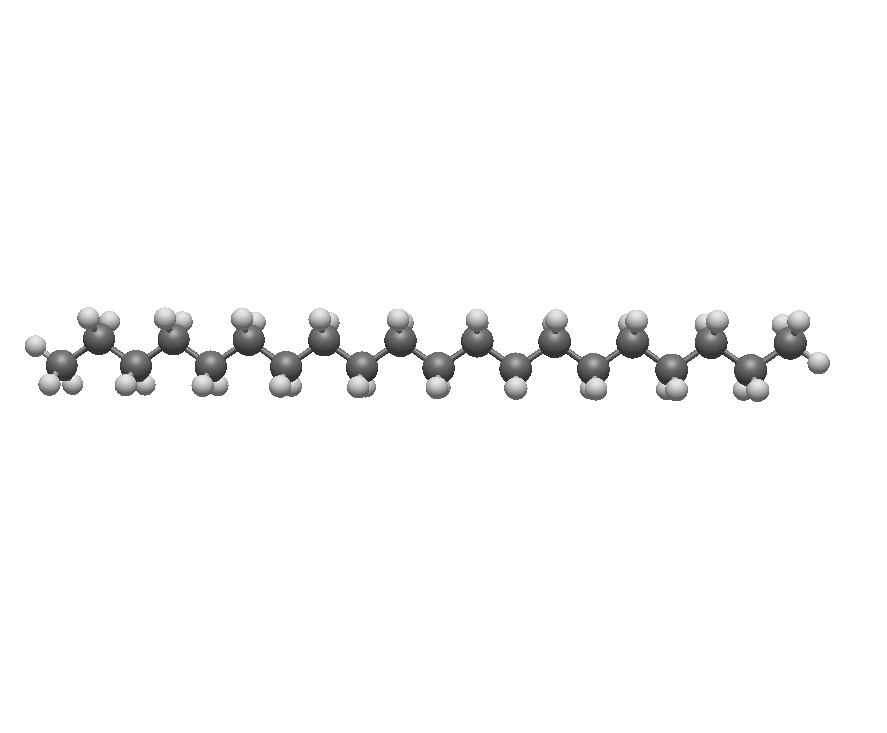
\includegraphics[width=\textwidth]{Pics/alkan.png}
         \caption{}
     \end{subfigure}
	\begin{subfigure}{0.5\textwidth}
         \centering
         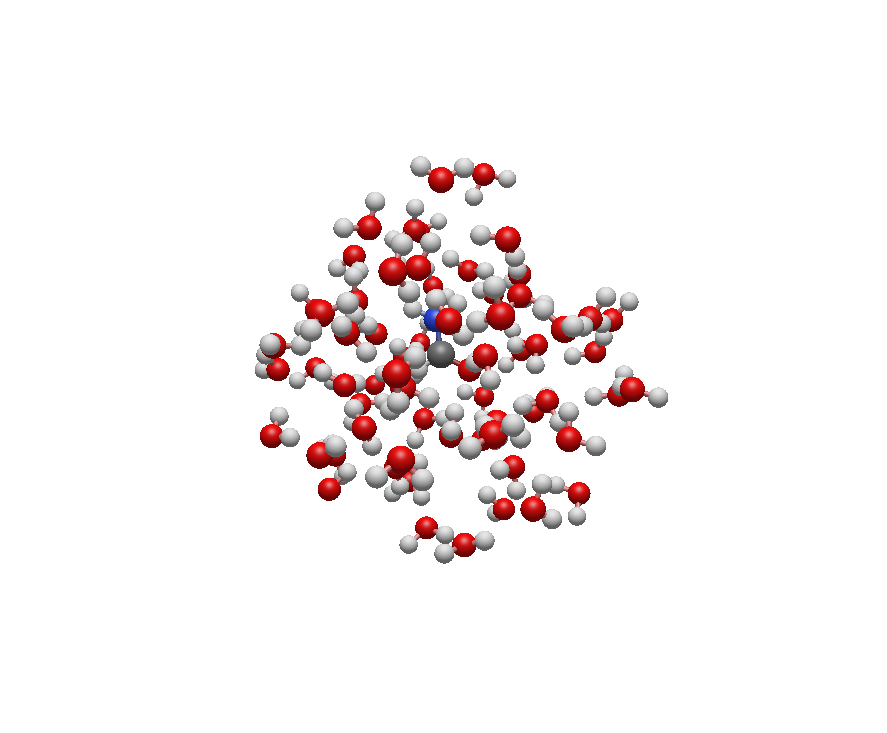
\includegraphics[width=\textwidth]{Pics/FW63.png}
         \caption{}
         \label{fig:five over x}
     \end{subfigure}
     	\caption{Molecular systems used for the analysis of the J, K and Z kernels: (a) linear alkanes (LA); (b) hydrated formamide (FW)}
        \label{fig:GS_MOL}
\end{figure}

\begin{table}
\centering
\begin{tabular}{llllll}
\hline
\multicolumn{3}{c}{LA} & \multicolumn{3}{c}{FW} \\ \hline
Molecule & Abbrev. & $N_{AO}$ & Molecule & Abbrev. $N_{AO}$ \\ \hline
H$_{42}$C$_{20}$ & LA20 & 490 & H$_{33}$CNO$_{16}$ & FW15 & 417 \\
H$_{82}$C$_{40}$ & LA40 & 970 & H$_{63}$CNO$_{31}$ & FW30 & 777 \\
H$_{162}$C$_{80}$ & LA80 & 1930 & H$_{129}$CNO$_{64}$ & FW63 & 1569  \\
H$_{322}$C$_{160}$ & LA160 & 3850 & H$_{291}$CNO$_{145}$ & FW144 & 3513 \\
\hline  
\end{tabular}
\caption{Molecular formula for the considered systems and the number of basis functions for cc-pVDZ. \label{tab:GS_NBAS}}
\end{table}

\subsection{Illustrating the Scaling}

There are generally two ways how scaling is illustrated in literature: (1) a graph that shows the total wall time as a function of increasing system size and/or (2) a table with scaling coefficients computed relative to a previous system size as
\begin{equation}
x = \frac{log(N_i/N_{i-1})}{log(T_i/T_{i-1})}
\end{equation} 
\noindent Graphs are most useful to show the prefactor of the methods, while tables are much better suited for showing the polynomial scaling, as the differences between e.g. $\ccpx{2}$ and $\ccpx{2.5}$ are difficult to pick up with the naked eye. Here, both methods are used. 

\FloatBarrier

\subsection{Integral Evaluation}

The J and K kernels have the tensors $B_{X\mu\nu}$ and $M_{XY}$ as common input. They are defined by
\begin{equation}
\cn{\mu\nu}{\lambda\sigma} = B_{X\mu\nu} M_{XY} B_{X\lambda\sigma}
\end{equation}
\noindent Three different density fitting approximations are considered for benchmarking: the standard density fitting in the coulomb metric (DFCM), local density fitting in the coulomb attenuated metric with the complimentary error function (DFCAM), and quasi-robust density fitting (QRDF). The exact form of $\mbf{B}$ and $\mbf{M}$ depends on the DF approximation (Table \ref{tab:BMTENSORS}). If not indicated otherwise, DFCAM uses an attenuation factor of 0.1, and QRDF uses $T$ = 1e-5 and $R$ = 40. 

\begin{table}
\centering
\begin{tabular}{lcc}
\hline
DF method & $B^X_{\mu\nu}$ & $M_{XY}$ \\
\hline
DFCM & $\cn{X}{\mu\nu}$ &  $\cn{X}{Y}^{-1}$ \\
DFCAM & $\cn{X}{\mu\nu}_{\omega}$ & $\cn{X}{Y}_{\omega}^{-1} \cn{Y}{R} \cn{R}{S}_{\omega}^{-1}$ \\
QRDF & $C^{QRDF}_{X\mu\nu}$ & $\cn{X}{Y}$ \\ 
\hline
\end{tabular}
\caption{Expressions for $\mbf{B}$ and $\mbf{M}$ for kernels presented in this work. The subscript $\omega$ indicates that the coulomb attenuated metric is used. \label{tab:BMTENSORS}}
\end{table}

Figure \ref{fig:GS_BTIME_ALKAN} shows the time needed to evaluate $\mbf{B}$ for the LA systems. There is no difference between DFCM and DFCAM, hence only DFCM is shown. QRDF has a much higher prefactor due to the huge number of QR decompositions that are necessary for the calculation of the fitting coefficients. The consequence is that QRDF is an order of magnitude more expensive than DFCM or DFCAM. Comparing the wall times here to the the total time needed for the Hartree-Fock procedure, QRDF is actually more expensive than the whole HF computation for LA20, LA40 and LA80. However, QRDF has the advantage of becoming linearly scaling going from LA80 to LA160, compared to the quadratic scaling of DFCM.  

In QRDF, the test functions $\{Q\}$ for the fitting procedure are chosen based on overlap criteria with the fitting functions $\{P\}$ (Equation \ref{eq:QRDF_TEST}). Here lies the reason for the massive overhead of QRDF: in the original implementation by Tew, the smallest exponent of a GTO is chosen for determining the overlap between $\mu_Q$ and $\nu_P$. In the QRDF procedure as implemented in \mchem{}, the scheme is generalized to \emph{blocks} of basis shells centered on the same atom, i.e. the smallest exponent of the whole block is used for the overlap screening. This had the unwanted side-effect that the screening for the test functions is much harsher than necessary. Even if the overlap values for most exponents of a block with another block are zero, only one exponent decides whether the block is included in the fitting procedure. A more lenient criteria based on an average overlap or matrix norm can reduce the overhead with little impact on accuracy. For most of this chapter, the original, strict version of the QRDF algorithm is used, but for determining the accuracy of CDD-DF-SOS-ADC(2), an improved version will be used (see below). The strictness of the method has no impact on the sparsity of the fitting coefficients, and hence all findings on the scaling of the kernels will still be valid for the new implementation.

Figure \ref{fig:GS_BNZE_ALKAN} shows the number of non-zero elements of $\mbf{B}$ for LA. Quadratic scaling can be observed for DFCM, and linear scaling for DFCAM and QRDF. An interesting observation is that $\mbf{B}$ is evaluated with $\ccpx{2}$ effort in DFCAM, but it scales linearly in its elements. This is due to the screening procedure: for DFCAM, the normal DFCM Schwarz screening is used, which does not take into account the $erfc(\omega r)/r$¨ decay between $\cbra{X}$ and $\cket{\mu\nu}$. More strict screening procedures could be introduced to speed up integral evaluation of DFCAM, which will be especially useful for direct algorithms. Similarly, the QRDF scheme has mostly cubic scaling effort for evaluation, but ultimately the elements scale linearly with system size. 

Finally, Figure \ref{fig:GS_BNZE_FW} shows the memory footprint of $\mbf{B}$ for the hydrated formamide systems. The tensors are naturally much more dense due to the molecular structure. Nonetheless, the QRDF fitting coefficients still scale quite favorably. Unfortunately, the QRDF procedure itself takes ten times longer than the HF calculation itself. Whether this is due to the strictness of QRDF, or just the nature of QRDF itself, is a point for further investigation. For now, QRDF is not considered useful for dense electronic systems. 

To compute $\mbf{M}$ in DFCM and DFCAM, a matrix inversion needs to computed, which scales with $\ccpx{3}$. For the system sizes considered in this report, the relative wall times for matrix inversions are small compared to all other steps. The QR decompositions in QRDF also scale cubically, although the size of the linear least squares problem will eventually become constant, i.e. the number of test functions will be independent of system sizes. This is a major advantage of QRDF, although as was already pointed out, it does matter for the current molecular sizes.

%%%%%%%%%%%%%%%%%%% MEMORY INTEGRALS (LA) %%%%%%%%%%%%%%%%%%%%%%%
\begin{figure}
\begin{subfigure}{\textwidth}

\begin{subfigure}{0.45\textwidth}
\vspace{0pt}
\centering
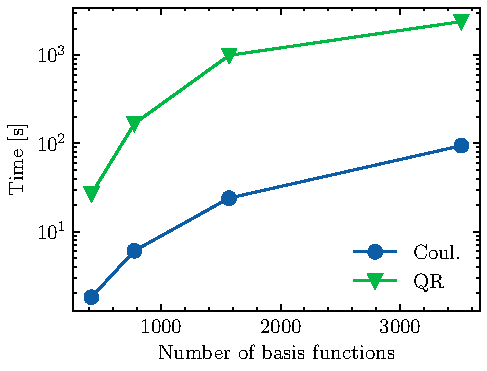
\includegraphics[width=\textwidth]{../articles/art1/qrtime_alkan}
%\captionof{figure}[This Figure]{Figure}
%\par
\end{subfigure}
\hfill
\begin{subtable}{0.45\textwidth}
\centering
\begin{tabular}{rrr}
\hline
N$_{AO}$ & DFCM & QRDF \\ \hline
490 & --- & --- \\ 
970 & 1.94 & 2.95 \\ 
1930 & 1.96 & 2.53 \\ 
3850 & 1.70 & 1.09 \\ \hline
\end{tabular}
%\captionof{table}[This Table]{Table}
%\par\vspace{0pt}
\end{subtable}
\caption{}
\label{fig:GS_BTIME_ALKAN}
\end{subfigure}

\vspace{1.5\baselineskip}

\begin{subfigure}{\textwidth}
\begin{subfigure}{0.45\textwidth}
\centering
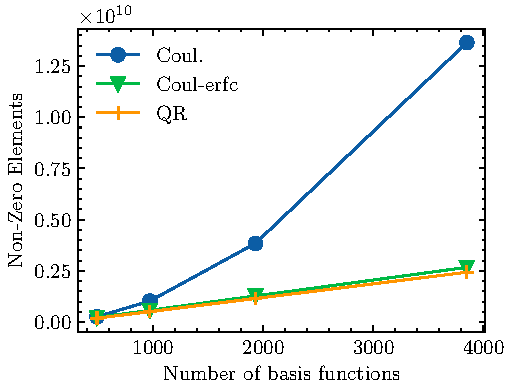
\includegraphics[width=\textwidth]{../articles/art1/eri_nze_alkan}
\end{subfigure}
\hfill
\begin{subtable}{0.45\textwidth}
\centering
\resizebox{\textwidth}{!}{
\begin{tabular}{rrrr}
\hline
N$_{AO}$ & DFCM & DFCAM & QRDF \\ \hline
490 & --- & --- & --- \\ 
970 & 2.01 & 1.37 & 1.45 \\ 
1930 & 1.92 & 1.16 & 1.18 \\ 
3850 & 1.83 & 1.07 & 1.08 \\ \hline
\end{tabular}
}
\end{subtable}
\caption{}
\label{fig:GS_BNZE_ALKAN}
\end{subfigure}

\vspace{1.5\baselineskip}

\begin{subfigure}{\textwidth}
\begin{subfigure}{0.45\textwidth}
\centering
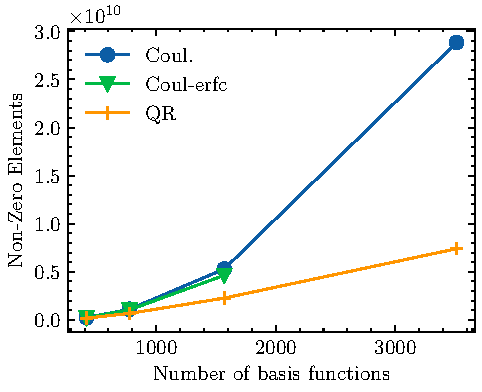
\includegraphics[width=\textwidth]{../articles/art1/eri_nze_fw}
%\captionof{figure}[This Figure]{Figure}
\end{subfigure}
\hfill
\begin{subtable}{0.45\textwidth}
\centering
\resizebox{\textwidth}{!}{
\begin{tabular}{rrrr}
\hline
N$_{AO}$ & DFCM & DFCAM & QRDF \\ \hline
417 & --- & --- & --- \\ 
777 & 2.50 & 2.45 & 2.15 \\ 
1569 & 2.23 & 2.11 & 1.73 \\ 
3513 & 2.10 & --- & 1.47 \\ \hline
\end{tabular}
}
%\captionof{table}[This Table]{Table}
\end{subtable}
\caption{}
\label{fig:GS_BNZE_FW}
\end{subfigure}
\caption{(a) Total walltime needed to construct the tensor $B_{X\mu\nu}$ (3c2e integrals, QR fitting coefficients) for LA, with scaling coefficients. (b) Number of non-zero elements in the tensor $B_{X\mu\nu}$ as a function of $N_{AO}$ for LA, with the corresponding scaling coefficients. (c) Number of non-zero elements in the tensor $B_{X\mu\nu}$ as a function of $N_{AO}$ for FW, with the corresponding scaling coefficients}
\end{figure}


%\caption{Total walltime needed to construct the tensor $B_{X\mu\nu}$ (3c2e integrals, QR fitting coefficients) for LA}
%\label{fig:GS_BTIME_ALKAN}
%\end{figure}
%
%\caption{Number of non-zero elements in the tensor $B_{X\mu\nu}$ as a function of $N_{AO}$ for LA, with the corresponding scaling coefficients}
%\label{fig:GS_BNZE_ALKAN}
%
%\caption{Number of non-zero elements in the tensor $B_{X\mu\nu}$ as a function of $N_{AO}$ for FW, with the corresponding scaling coefficients}
%\label{fig:GS_BNZE_FW}

\subsection{Hartree-Fock}

\subsubsection{Scaling: Coulomb Matrix}

The coulomb matrix is evaluated as
\begin{align}
d_X = M_{XY} B_{Y\mu\nu} P_{\nu\mu} \\
J_{\mu\nu} = B_{X\mu\nu} d_X
\end{align}
\noindent The scaling of the individual steps is not considered, but only the total time needed to construct the coulomb matrix. Figure \ref{fig:GS_DFJSCALE_LA} shows the scaling behavior of the J kernel for the LA systems. DFCM does not lower the scaling compared to the exact evaluation of the coulomb matrix which scales quadratically if sparse matrix algebra is used. Local metrics can however lower the scaling by an order of magnitude. QRDF even exhibits sublinear scaling from LA80 to LA160. The sublinear scaling originates from the increased sparsity of $\mbf{M}$. While DFCM and DFCAM need to invert matrices, which also destroys sparsity, QRDF only needs the 2c2e integrals which have an $1/R^{l+1}$ decay between centers. Although this decay is slow, it is faster compared to the 4c2e integrals and can affect the scaling positively.

Table \ref{tab:GS_DFJKSCALE_FW} shows the scaling coefficients for the FW systems. Here, DFCAM and QRDF do not give any considerable advantage over DFCM. %(ABSOLUTE???)

\subsubsection{Scaling: Exchange Matrix}

The exchange matrix is computed as
\begin{align}
C_{X\mu\nu} &= M_{XY} B_{Y\mu\nu} \\
K_{\mu\nu} &= B_{X\nu\sigma} C_{X\mu\lambda} P_{\lambda\sigma} 
\end{align}
\noindent Both steps are analyzed separately. Step 1 actually only needs to be evaluated once, while step 2 is repeated at each iteration. Figure \ref{fig:GS_DFK1SCALE_LA} illustrates the scaling for step 1 for linear alkanes. It is the most expensive step of the Hartree-Fock procedure in terms of scaling (ignoring diagonalization and matrix inversion), and profits most from the local density fitting approximation. The computational effort can be reduced to $\ccpx{2}$ and almost $\mathcal{O}(N)$ for QRDF. Step 1 forms a 3-index tensor which needs to be stored in memory. The sparsity of this tensor is illustrated in Figure \ref{fig:GS_MBNZE_LA}. The number of elements scales approximately quadratically for all metrics, although QRDF has a slight edge on the other methods. It appears that local density fitting approximations do not have a lot of impact on the memory requirements of step 1, although they can speed up the computation considerably. 

Step 2 is less expensive, but still more demanding than the computation of the coulomb matrix. Figure \ref{fig:GS_DFK2SCALE_LA} shows the scaling for linear alkanes. Moreover, the MO algorithm is also included for comparison. Even standard density fitting can positively impact the scaling, with a reduction from cubic to $\ccpx{1.5}$. DFCAM does not improve on the scaling, although the additional sparsity lowers the prefactor compared to DFCM. QRDF can again achieve linear scaling, for similar reasons as discussed above. 

%%%%%%%%%%%%%%%%% SCALING (LA) %%%%%%%%%%%%%%%%%%%%
\begin{figure}[htp]

\begin{subfigure}{\textwidth}
\begin{subfigure}{0.45\textwidth}
\centering
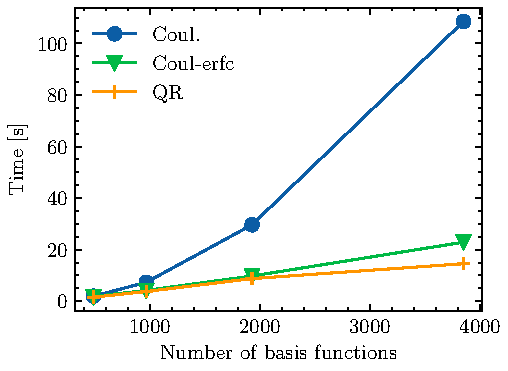
\includegraphics[width=\textwidth]{../articles/art1/hfJ_alkan}
%\label{fig:GS_DFJSCALE_LA}
\end{subfigure}
\hfill
\begin{subtable}{0.45\textwidth}
\centering
\begin{tabular}{rrrr}
\hline
N$_{AO}$ & DFCM & DFCAM & QRDF \\ \hline
490 & --- & --- & --- \\ 
970 & 1.93 & 1.23 & 1.29 \\ 
1930 & 2.03 & 1.23 & 1.23 \\ 
3850 & 1.88 & 1.23 & 0.73 \\ \hline
\end{tabular}
\end{subtable}
\caption{}
%Scaling behavior for the construction of the coulomb matrix using different metrics (LA)}
\label{fig:GS_DFJSCALE_LA}
\end{subfigure}

\vspace{1.5\baselineskip}

\begin{subfigure}{\textwidth}
\begin{subfigure}{0.45\textwidth}
\centering
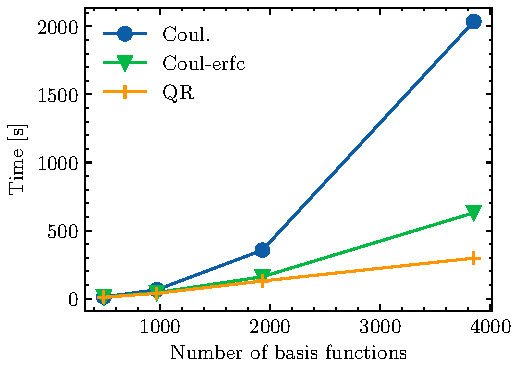
\includegraphics[width=\textwidth]{../articles/art1/hfK1_alkan}
\end{subfigure}
\hfill
\begin{subtable}{0.45\textwidth}
\centering
\begin{tabular}{rrrr}
\hline
N$_{AO}$ & DFCM & DFCAM & QRDF \\ \hline
490 & --- & --- & --- \\ 
970 & 2.43 & 1.97 & 1.96 \\ 
1930 & 2.49 & 1.89 & 1.78 \\ 
3850 & 2.53 & 1.98 & 1.21 \\ \hline
\end{tabular}
\end{subtable}
\caption{}
%Scaling behavior for the construction of the exchange matrix (step1) using different metrics (LA)}
\label{fig:GS_DFK1SCALE_LA}
\end{subfigure}

\vspace{1.5\baselineskip}

\begin{subfigure}{\textwidth}
\begin{subfigure}{0.45\textwidth}
\centering
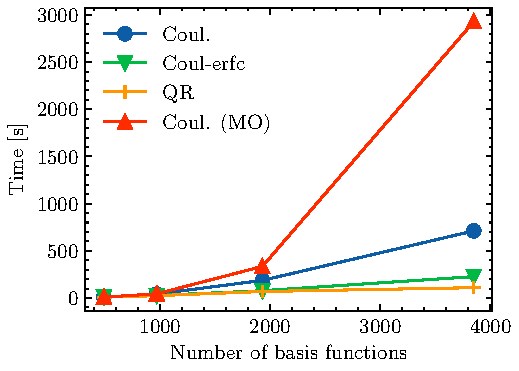
\includegraphics[width=\textwidth]{../articles/art1/hfK2_alkan}
\end{subfigure}
\hfill
\begin{subtable}{0.45\textwidth}
\centering
\resizebox{\textwidth}{!}{
\begin{tabular}{rrrrr}
\hline
N$_{AO}$ & DFCM & DFCAM & QRDF & DFMO \\ \hline
490 & --- & --- & --- & --- \\ 
970 & 1.58 & 1.58 & 1.60 & 2.34 \\ 
1930 & 1.57 & 1.57 & 1.50 & 2.96 \\ 
3850 & 1.56 & 1.56 & 0.67 & 3.14 \\ \hline
\end{tabular}
}
\end{subtable}
\caption{}
%Scaling behavior for the construction of the exchange matrix (step 2) using different metrics (LA)}
\label{fig:GS_DFK2SCALE_LA}
\end{subfigure}
\caption{(a) Scaling behavior for the construction of the coulomb matrix using different metrics (LA). (b) Scaling behavior for the construction of the exchange matrix (step1) using different metrics (LA). (c) Scaling behavior for the construction of the exchange matrix (step 2) using different metrics (LA)}
\end{figure}

%%%%%%%%%%%%%%%%% SCALING (FW) %%%%%%%%%%%%%%%%%%%%%%%

\begin{figure}[htp]

\begin{subtable}{\textwidth}
\resizebox{\textwidth}{!}{
\begin{tabular}{r|rrr|rrr|rrrr}
\hline
 & \multicolumn{3}{c}{J} & \multicolumn{3}{c}{K (STEP 1)} &   \multicolumn{4}{c}{K (STEP 2)} \\ \hline
N$_{AO}$ & DFCM & DFCAM & QRDF & DFCM & DFCAM & QRDF & DFCM & DFCAM & QRDF & DFMO \\ \hline
417 & --- & --- & --- & --- & --- & --- & --- & --- & --- & --- \\ 
777 & 2.18 & 2.20 & 1.88 & 2.77 & 2.77 & 2.51 & 2.55 & 2.55 & 2.33 & 2.33 \\ 
1569 & 2.32 & 1.71 & 1.28 & 2.77 & 2.18 & 1.85 & 2.82 & 2.13 & 1.67 & 2.86 \\ 
3513 & 2.08 & --- & 1.94 & 2.79 & --- & 2.74 & 2.59 & --- & 2.65 & 3.13 \\ \hline
\end{tabular}
}
\caption{}
\label{tab:GS_DFJKSCALE_FW}
\end{subtable}

\vspace{1.5\baselineskip}

\begin{subfigure}{\textwidth}
\centering
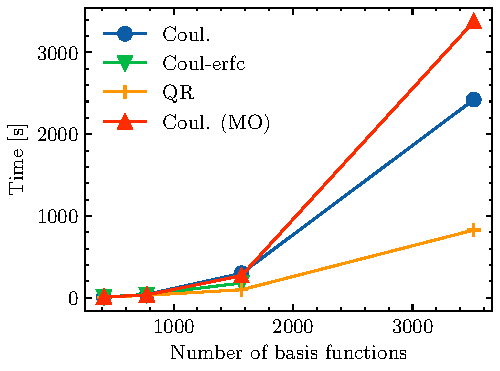
\includegraphics[scale=1.0]{../articles/art1/hfK2_fw}
\caption{}
\label{fig:GS_DFK2SCALE_FW}
\end{subfigure}

\caption{(a) Scaling coefficients for the J kernel and the two steps of the K kernel (FW). (b) Scaling for the construction of the exchange matrix (step 2) for hydrated formamide. Although local density approximations do not lower the scaling, a reduction of the prefactor can be observed.}

\end{figure}

%%%%%%%%%%%%%%%%% MEMORY (LA/FW) %%%%%%%%%%%%%%%%%%%%%%%%

%
\begin{figure}[htp]

\begin{subfigure}{\textwidth}
\begin{subfigure}{0.45\textwidth}
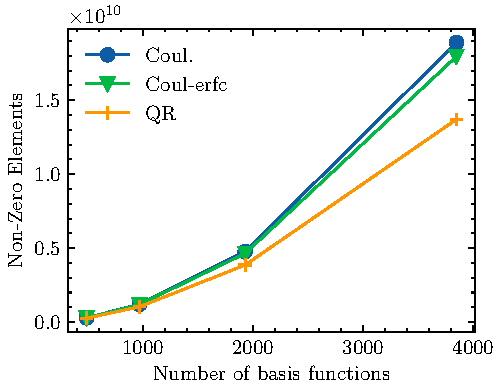
\includegraphics[width=\textwidth]{../articles/art1/cfit_nze_alkan}
\end{subfigure}
\hfill
\begin{subtable}{0.45\textwidth}
\begin{tabular}{rrrr}
\hline
N$_{AO}$ & DFCM & DFCAM & QRDF \\ \hline
490 & --- & --- & --- \\ 
970 & 2.07 & 2.06 & 2.01 \\ 
1930 & 2.01 & 1.98 & 1.92 \\ 
3850 & 1.99 & 1.96 & 1.84 \\ \hline
\end{tabular}
\end{subtable}
\caption{}
\label{fig:GS_MBNZE_LA}
\end{subfigure}

\vspace{1.5\baselineskip}

\begin{subfigure}{\textwidth}
\begin{subfigure}{0.45\textwidth}
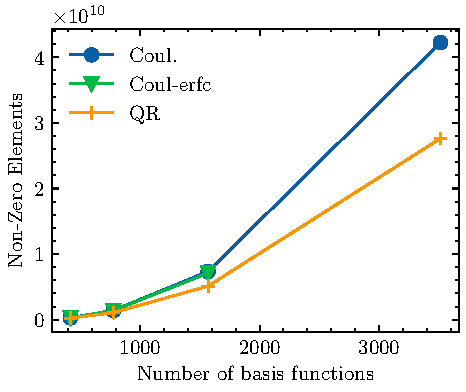
\includegraphics[width=\textwidth]{../articles/art1/cfit_nze_fw}
\end{subfigure}
\hfill
\begin{subtable}{0.45\textwidth}
\begin{tabular}{rrrr}
\hline
N$_{AO}$ & DFCM & DFCAM & QRDF \\ \hline
417 & --- & --- & --- \\ 
777 & 2.27 & 2.26 & 2.20 \\ 
1569 & 1.96 & 1.94 & 1.88 \\ 
3513 & 1.71 & 1.68 & 1.57 \\ \hline
\end{tabular}
\end{subtable}
\caption{}
\label{fig:GS_MBNZE_FW}
\end{subfigure}
%

\caption{(a) Scaling behavior of the tensor $M_{XY}B_{Y\mu\nu}$. (b) Scaling behavior of the tensor $M_{XY}B_{Y\mu\nu}$ (FW).}

\end{figure}

Finally, the scaling coefficients for the FW systems are collected in Table \ref{tab:GS_DFJKSCALE_FW}. As expected, local density fitting does not considerably reduce the scaling for evaluating the exchange matrix and shows the limit of what AO methods can do. Of course, at some point, the computational effort will eventually decrease with increasing system size $N$, although the crossover point is much later than for LA. The major advantage is that, compared to a MO implementation, local density fitting decreases the overhead compared to DFCM, making it more competitive to the MO methods (Figure \ref{fig:GS_DFK2SCALE_FW}). The AO method is therefore still applicable in a dense context. 

For FW, numerical issues were encountered for FW144, hence this point is missing in the tables and figures.

\subsubsection{Accuracy}

The accuracy of the J and K kernels are compared collectively by considering the total Hartree Fock energy. Table \ref{tab:GSHFACCURACY} lists the total energy differences per occupied orbital in $\mu$Hartrees for a small set of molecules. Here, LA30 and FW21 are introduced, with the respective molecular formulas H$_{62}$C$_{30}$ and H$_{45}$CO$_{22}$. For standard density fitting, one finds errors on the order of several $\mu$Hartrees, which is in accordance to results in literature. QRDF has virtually the same errors compared to DFCM, although this might also be partly due to the strict screening of test functions. DFCAM unfortunately shows very large errors that are two orders of magnitude larger than QRDF and DFCM. Here lies yet another advantage of the QRDF scheme: while Dunlap's robust density fitting is crucial for obtaining accurate results for local density fitting approximations like DFCAM, QRDF has no such restrictions. 

\begin{table}[h!]
\centering
\begin{tabular}{cccc}
 \hline
 & DFCM & DFCAM & QRDF \\ \hline 
LA20 & 3.76 & 235.21 & 3.80 \\ 
LA30  & 3.85 & 274.59 & 3.85 \\ 
LA40 & 3.85 & 368.60 & 3.84 \\ 
FW15 & 8.23 & 713.43 & 8.21 \\ 
FW21 & 7.95 & 524.92 & 7.95 \\ 
FW30 & 1.59 & 111.87 & 1.59 \\ 
\hline 
\end{tabular}
\caption{Absolute Hartree-Fock energy difference in $\mu$Hartrees per occupied orbital compared to exact Hartree-Fock.}
\label{tab:GSHFACCURACY}
\end{table}

\FloatBarrier

\subsection{MP2}

\subsubsection{Scaling}

The Z kernel is defined here as
\begin{align}
D\pa_{X\ulgm\olgn} &= L\pa_{\mu\oli} \left( L\pa_{\mu' \oli} B_{X\mu'\nu'}  Q\pa_{\nu'\nu} \right) \\
Z_{XY}\pa &= D\pa_{X\ulgm\olgn} B_{Y\mu\nu}
\end{align}
\noindent and is evaluated for each Laplace point $\alpha$. The 3-index intermediate $\mbf{D}$ can either be stored in main memory, stored on disk, or computed on the fly. Here, only the first variant of the algorithm is considered, although the other methods are implemented as well. First, the sparsity of the intermediate tensor will be considered (Figure \ref{fig:GS_ZMEM_LA}) for the LA systems. Quadratic scaling is observed for DFCM, while linear scaling is achievable for DFCAM and QRDF. This is in accordance to the sparsity analysis in chapter 4. Again, local density fitting is crucial to reduce the memory footprint.

\begin{figure}[htp]

\begin{subfigure}{\textwidth}
\begin{subfigure}{0.45\textwidth}
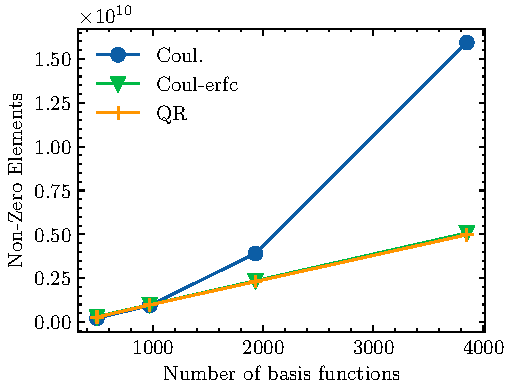
\includegraphics[width=\textwidth]{../articles/art1/ftmp2_nze_alkan}
\end{subfigure}
\hfill
\begin{subtable}{0.45\textwidth}
\begin{tabular}{rrrr}
\hline
N$_{AO}$ & DFCM & DFCAM & QRDF \\ \hline
490 & --- & --- 	& --- \\ 
970	& 2.14 & 1.69 & 1.80 \\
1930	 & 2.06 & 1.26 & 1.25 \\
3850	 & 2.03 & 1.11 & 1.11 \\
 \hline
\end{tabular}
%\captionof{table}[This Table]{REDO THIS!!!!}
\end{subtable}
\caption{}
\label{fig:GS_ZMEM_LA}
\end{subfigure}

\vspace{1.5\baselineskip}

\begin{subfigure}{\textwidth}
\begin{subfigure}{0.45\textwidth}
\centering
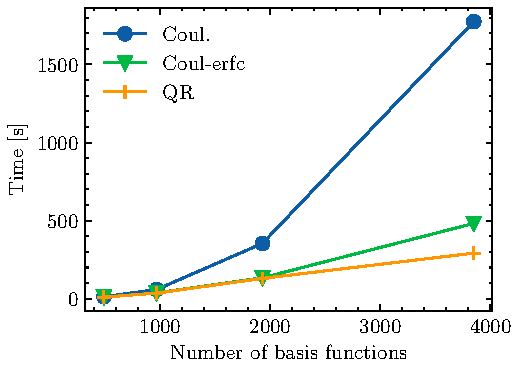
\includegraphics[width=\textwidth]{../articles/art1/mp2_alkan}
%\captionof{figure}[This Figure]{Figure}
\end{subfigure}
\hfill
\begin{subtable}{0.45\textwidth}
\centering
\begin{tabular}{rrrr}
\hline
N$_{AO}$ & DFCM & DFCAM & QRDF \\ \hline
490 & --- & --- 	& --- \\ 
970	& 2.45 & 1.96 & 2.09 \\
1930	 & 2.55 & 1.82 & 1.83 \\
3850	 & 2.00 & 1.59 & 1.00 \\
 \hline
\end{tabular}
%\captionof{table}[This Table]{REDO THIS!!!!}
\end{subtable}
\caption{}
\label{fig:GS_ZSCALE_LA}
\end{subfigure}

\vspace{1.5\baselineskip}

\begin{subfigure}{\textwidth}
\begin{subfigure}{0.45\textwidth}
\centering
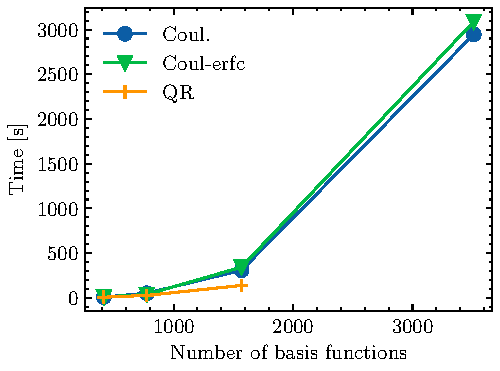
\includegraphics[width=\textwidth]{../articles/art1/mp2_fw}
%\captionof{figure}[This Figure]{Figure}
\end{subfigure}
\hfill
\begin{subtable}{0.4\textwidth}
\centering
\begin{tabular}{rrrr}
\hline
N$_{AO}$ & DFCM & DFCAM & QRDF \\
\hline 
490 & --- & --- & --- \\ 
970 & 2.51 & 1.88 & 1.88 \\ 
1930 & 2.59 & 3.18 & 2.36 \\ 
3850 & 3.26 & 3.18 & --- \\ 
 \hline
\end{tabular}
%\captionof{table}[This Table]{REDO THIS!!!!}
\end{subtable}
\caption{}
\label{fig:GS_ZSCALE_FW}
\end{subfigure}

\caption{(a) Sparsity behavior of the intermediate tensor $\mbf{D}$ in the Z kernel for the first Laplace point. (b) Average wall times for the construction of the Z kernel and scaling coefficients (LA). (c) Average wall times for the construction of the Z kernel and scaling coefficients (FW).}

\end{figure}

The scaling behavior of the Z kernel is collected in Figure \ref{fig:GS_ZSCALE_LA} for LA. Even with DFCM, the computational effort is drastically reduced from quartic to quadratic. It is even further reduced with LDF, and linear scaling of the Z kernel is obtained for QRDF from LA80 to LA160. 

For the hydrated formamide systems, scaling is again less favorable (Figure \ref{fig:GS_ZSCALE_FW}). Nonetheless, it still scales at $\ccpx{3}$, i.e. one order of magnitude less than the canonical algorithm. As opposed to HF, LDF has no major impact on the prefactor. The last point for FW163 is missing for QRDF due to numerical issues.  

\subsubsection{Accuracy}

The accuracy for the different density fitting approximations is given in Table \ref{fig:GS_ZACCURACY}, compared to the canonical SOS-MP2, in $\mu$Hartrees per occupied orbital. For all methods, the Hartree-Fock reference is calculated with DFCM.

Immediately, it is apparent that the energy errors are much higher than for Hartree-Fock. This is due to the quality of the HF wave function, which was computed using density fitting. Results may be improved by using a larger auxiliary basis set to improve the description of the virtual space. The impact of the HF wave function on the SOS-MP2 energy is not explored here.

DFCM, DFCAM and QRDF all have similar errors. The SOS-MP2 energy is therefore much less sensitive to the density fitting approximation, because it is a non-iterative method and DFCAM can be used without problems in this case. 

\begin{table}[h]
\centering
\begin{tabular}{cccc}
 \hline
 & Coul. & Coul-erfc & QR\\ \hline 
alkan20 & 28.81 & 28.76 & 28.85 \\ 
alkan30  & 29.04 & 29.02 & 29.14 \\ 
alkan40 & 28.38 & 28.38 & 28.50 \\ 
FW15 & 23.31 & 23.29 & 23.27 \\ 
FW21 & 23.27 & 23.26 & 23.26 \\ 
FW30 & 24.30 & 24.20 & 24.10 \\ 
\hline 
\end{tabular}
\caption{SOS-MP2 energy differences in $\mu$Hartrees per occupied orbital compared to the canonical SOS-MP2 reference.}
\label{fig:GS_ZACCURACY}
\end{table}

\section{CDD-DF-SOS-ADC(2)}

\subsection{Molecular Test Systems}

For the performance analysis of CDD-DF-SOS-ADC(2), again two molecular systems are chosen: linear carboxylic acids (LCA, Figure \ref{fig:ACID}) and the hydrated formamide systems (FW) from the previous section. The LCAs were optimized using DFT/B3LYP and the 6-31G* basis set.

Two major factors influence the performance of local excited state methods: locality of electron correlation, and locality of the excitation space. The LCA systems form the best case scenario for both types of locality. The atomic ground state density becomes sparse very rapidly with increasing chain length, and so does the atomic transition density for the lowest lying singlet excitation. The excitation space for that transition is localized on the COOH group, and the number of elements in the transition density matrix scales with with $\mathcal{O}(1)$ in the limit of large systems. On the other hand, FW has a non-sparse AO ground state density, but a sparse AO transition density. Here, the first singlet excited state is localized on the formamide molecule. With increasing size of the solvation shell, the number of significant elements in the transition matrix grows slowly, and the excitation energy will eventually converge to a constant value in the limit of an infinitely large solvation shell \cite{Bau2017}, demonstrating the intensive property of excitations. As such, while FW is a worst case scenario for local ground state calculations, excited state methods are able to exploit the locality of the excitation in order to lower the computational cost.   

\begin{figure}
\centering
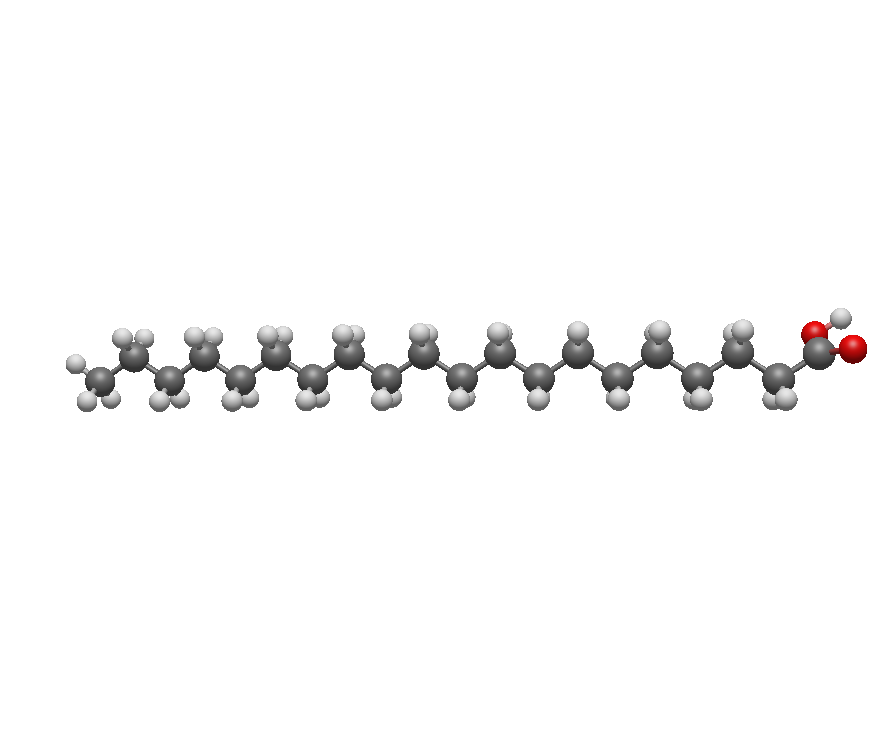
\includegraphics[width=0.5\textwidth]{Pics/acid.png}
\caption{Structure of the linear carboxylic acids (LCA).}
\label{fig:ACID}
\end{figure}

\subsection{Scaling}

For analyzing the scaling of the AO-ADC(2) method, the cc-pVDZ basis set is used, with cc-pVDZ-ri for density fitting. Table \ref{tab:ES_NUMBAS} shows the number of basis functions for the test systems. Furthermore, only the performance of the first matrix-vector product is analyzed, using a (singlet) CIS-optimized transition matrix as the input. The CIS vectors are sparse, and the density of the ADC(2) trial vectors will be of similar sparsity. It should be noted that it is very important to use CIS as the the initial guess, because a guess based on molecular orbital energies can be very dense. 

\begin{table}[h]
\centering
\begin{tabular}{llllll}
\hline
\multicolumn{3}{c}{LCA} & \multicolumn{3}{c}{FW} \\ \hline
Molecule & Abbrev. & $N_{AO}$ & Molecule & Abbrev. & $N_{AO}$ \\ \hline
H$_{41}$C$_{20}$O & LCA20 & 508 & H$_{33}$CNO$_{16}$ & FW15 & 417 \\
H$_{81}$C$_{40}$O & LCA40 & 988 & H$_{63}$CNO$_{31}$ & FW30 & 777 \\
H$_{161}$C$_{80}$O & LCA80 & 1948 & H$_{129}$CNO$_{64}$ & FW63 & 1569 \\
H$_{321}$C$_{160}$O & LCA160 & 3868 & H$_{291}$CNO$_{145}$ & FW144 & 3513 \\
\hline
\end{tabular}
\caption{Total number of basis functions for linear carboxylic acids (LCA) and solvated formamide (FW) with the aug-cc-pVDZ basis set}
\label{tab:ES_NUMBAS}
\end{table}

For evaluating the doubles part of the MVP, the OV version of the algorithm will be used.

Figure \ref{fig:ES_TIME_LCA} shows the performance of the matrix-vector product for the LCA systems. Again, three metrics are used: DFCM, DFCAM ($\omega$ = 0.1) and QRDF ($T$ = 1e-5, $R$ = 40). The atomic orbital formulation of ADC(2) drastically reduces the scaling from $\ccpx{4}$ to $\ccpx{2}$ for standard density fitting. Using local density fitting, the computational effort can be further pushed down to $\ccpx{1.5}$ and $\ccpx{1}$ for DFCAM and QRDF respectively. The cross-over is very early, and sub-quadratic scaling is already reached at LCA40. The performance of AO-ADC(2) is therefore even better than the predicted $\ccpx{2}$ scaling. This discrepancy is due to the sparsity of the AO transition matrix: during the sparsity analysis, $\ccpx{1}$ scaling was assumed, analogous to the ground state density. However, the transition density scales with $\mathcal{O}(1)$ in the asymptotic limit, which leads to sub-quadratic performance.

Figure \ref{fig:ES_TIMESINGLE_LCA} shows the total wall time for each individual component of the MVP calculation. The evaluation of the intermediate matrices (intermeds) and the doubles-part (2E) are the most expensive steps. The computational timings for computing part 2C, 2D and the CIS Fock matrices (jk) are one order of magnitude lower. Part 2A and 2B only involve a single matrix multiplication of the MO transition matrix with the intermediate matrices, and are therefore evaluated very quickly. The Cholesky decompositions also do not considerably influence the total scaling. 

Concerning the memory footprint of AO-ADC(2), the same 3-index tensors that appeared in the evaluation of the Hartree-Fock and SOS-MP2 ground state energy also appear here: $B_{X\mu\nu}$ (the 3c2e integrals or the QRDF fitting coefficients), $C_{X\mu\nu}$ (which corresponds to $M_{XY}B_{Y\mu\nu}$) and $B\pa_{X\uli\ola}$ (the pseudo-AO integrals $P\pa_{\mu\mu'} B_{X\mu'\nu'} Q\pa_{\nu'\nu}$). Their sparsity was discussed in detail in the previous section. Additionally, the following tensors need to be stored in memory: $C'_{X\mu\nu}$ ($G_{XY}B_{Y\mu\nu}$ in the K kernel during evaluation of the intermediates, see Algorithm 2), and the intermediate Laplace tensors in the Cholesky MO basis ($B\pt_{X\uli\ola}$, $R\pt_{X\uli\ola}$, $D\pt_{X\uli\ola}$), as defined in the previous chapter in Algorithm 6. The tensors will be abbreviated as $C'$, $B_{MO}$, $R_{MO}$ and $D_{MO}$ for this discussion, and $B_{AO}$ is used for $B_{X\mu\nu}$.

\ref{fig:ES_SPARSITY_LCA} shows the block sparsity of those tensors for QRDF, with $B_{AO}$ as a reference. Block sparsity is defined as the number of significant blocks divided by the total number of blocks in the dense tensor. $C'$ and $B_{MO}$ are very dense, with a block sparsity slightly below 10\%. The intermediate Laplace tensors $D_{MO}$ and $R_{MO}$ decay much faster than $B_{AO}$ which was shown to scale with $\mathcal{O}(N)$. For LCA160, $I_{MO}$ and $R_{MO}$ are an order of magnitude sparser ($\approx$ 0.1\%) than $B_{AO}$. The difference to the other Laplace tensor $B_{MO}$ is that $I_{MO}$ and $R_{MO}$ are formed by the contraction of $B_{AO}$ with both the AO ground state density $\mbf{P}$ and the AO transition matrix $\mbf{U}$, which explains their much higher degree of sparsity compared to $B_{MO}$ which is formed using the AO ground state densities only. One peculiar thing to notice here is that the intermediate tensor $D_{MO}$, which is formed from $B_{MO}$ and $R_{MO}$, is sparser than both of its input tensors. This indicates a potentially faster route to evaluating $D_{MO}$ by imposing sparsity criteria on $B_{MO}$ and $R_{MO}$. How these criteria exactly look like is subject of future investigation. The most plausible route goes via a sparsity analysis of the trial vector $u$, similar to how LMO or NO excited state methods generate a compact virtual orbital space.

\begin{figure}[htp]

\begin{subfigure}{\textwidth}
\begin{subfigure}{0.45\textwidth}
\centering
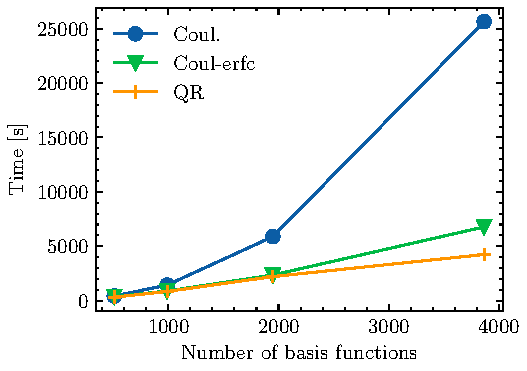
\includegraphics[width=\textwidth]{Pics/adctime_acid}
%\captionof{figure}[This Figure]{Figure}
\end{subfigure}
\hfill
\begin{subtable}{0.45\textwidth}
\centering
\begin{tabular}{rrrr}
\hline
N$_{AO}$ & DFCM & DFCAM & QRDF \\ \hline
508 & --- & --- & --- \\ 
988 & 1.8 & 1.4 & 1.5 \\ 
1948 & 2.1 & 1.5 & 1.4 \\ 
3868 & 2.2 & 1.5 & 1.0 \\
 \hline
\end{tabular}
%\captionof{table}[This Table]{REDO THIS!!!!}
\end{subtable}
\caption{}
\label{fig:ES_TIME_LCA}
\end{subfigure}

\vspace{1.5\baselineskip}

\begin{subfigure}{0.45\textwidth}
\centering
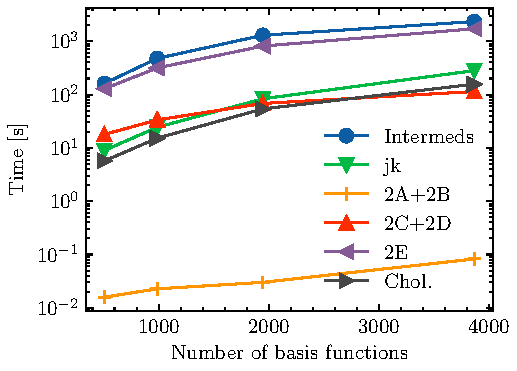
\includegraphics[width=\textwidth]{Pics/adcsingle_acid}
\caption{}
\label{fig:ES_TIMESINGLE_LCA}
\end{subfigure}
\hfill
\begin{subfigure}{0.45\textwidth}
\centering
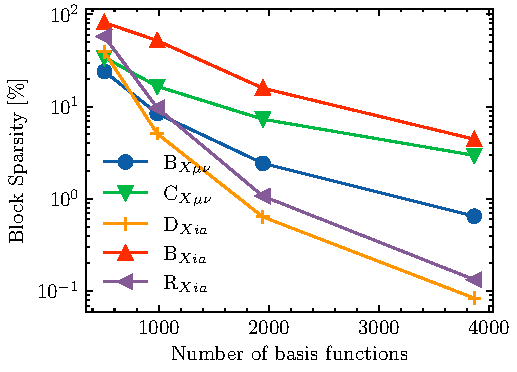
\includegraphics[width=\textwidth]{Pics/blocksparsity_acid}
\caption{}
\label{fig:ES_SPARSITY_LCA}
\end{subfigure}

\caption[Scaling behavior of CDD-DF-SOS-ADC(2) for LCA]{(a) Scaling behavior for the computation of a single matrix-vector-product with a CIS optimized (singlet) trial vector (LCA). (b) Total time needed to evaluate each separate component of the MVP using quasi-robust density fitting (LCA). (c) Block sparsity for the major 3-index tensors appearing in the evaluation of the MVP (LCA).}

\end{figure}

\begin{figure}

\begin{subfigure}{\textwidth}
\begin{subfigure}{0.45\textwidth}
\centering
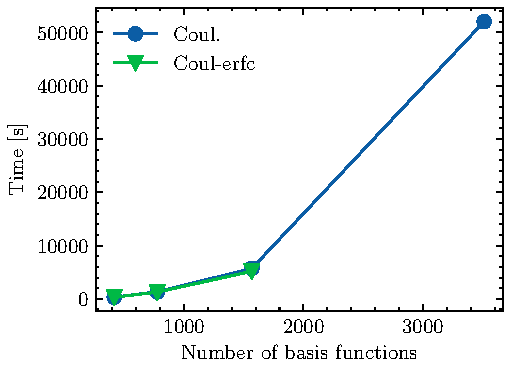
\includegraphics[width=\textwidth]{Pics/adctime_fw}
%\captionof{figure}[This Figure]{Figure}
\end{subfigure}
\hfill
\begin{subtable}{0.45\textwidth}
\centering
\begin{tabular}{rrr}
\hline
N$_{AO}$ & DFCM & DFCAM \\ \hline
508	& ---	& --- \\
988	& 2.3	& 2.3 \\
1948 & 	2.1 &	2.0 \\
3868	 & 2.74 & --- \\
 \hline
\end{tabular}
\end{subtable}
\caption{}
\label{fig:ES_TIME_FW}
\end{subfigure}

\vspace{1.5\baselineskip}

\centering
\begin{subfigure}{0.45\textwidth}
\centering
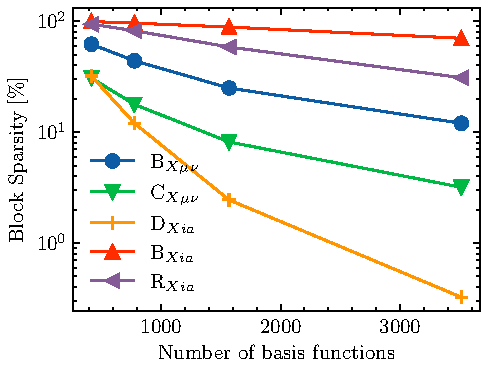
\includegraphics[width=\textwidth]{Pics/blocksparsity_fw}
\caption{}
\label{fig:ES_SPARSITY_FW}
\end{subfigure}

\caption[Scaling behavior of CDD-DF-SOS-ADC(2) for FW]{(a) Scaling behavior for the computation of a single matrix-vector-product with a CIS optimized (singlet) trial vector (FW). (b) Block sparsity for the major 3-index tensors appearing in the evaluation of the MVP (FW)}

\end{figure}

Similarly, the evaluation of the intermediate tensors can be sped up by only taking into the account the AOs which are near or within the excitation space. This would however lead to a loss of state specificity of the CDD-DF-SOS-ADC(2) MVP. 

Figure \ref{fig:ES_TIME_FW} shows the performance of CDD-DF-SOS-ADC(2) for solvated formamide. Although the density of the systems negatively impacts performance compared to LCA, it is still possible to achieve sub-cubic scaling thanks to the sparsity of the AO transition matrix. The point for FW144 with DFCAM is missing due to numerical issues that were encountered during the calculation. Nonetheless, the graph speaks for the success of the AO-ADC(2), even for non-ideal systems, provided that the excitation space is small. Figure \ref{fig:ES_SPARSITY_FW} shows the block sparsity of the tensors discussed in the previous paragraphs for LCA. Although most tensors are very dense, the intermediate $D_{MO}$ almost falls below the 0.1\% mark. Similarly to LCA, this sparsity might be used for imposing conditions on the other tensors, and speeding up the calculations for all components of the MVP. 

\subsection{Accuracy}

To get an impression on the accuracy that can be achieved with CDD-DF-SOS-ADC(2), the lowest lying singlet excitation energies for a small set of molecules are compared to the exact results obtained with canonical SOS-ADC(2), as implemented in Q-Chem. The Hartree-Fock wave function is optimized using standard density fitting without any local approximations as the reference for CDD-DF-SOS-ADC(2), while the exact HF ground state is used for the canonical calculation. The aug-cc-pVDZ basis set, and the auxiliary basis sets cc-pVTZ-jkfit and aug-cc-pVDZ-ri are used for Hartree-Fock and CDD-DF-SOS-ADC(2) respectively. The test systems include linear alkanes and carboxylic acids, solvated formamide, as well as the borondipyrromethene-flavin dyad (FLVA) \cite{Kat2007} and the phenothiazine-isoalloxazine dyad (DYAP) \cite{Cra2002}. The structures of FLVA and DYAP are given in Figure \ref{fig:FLVADYAP}.

%  Kats, D.; Korona, T.; Schütz, M. Transition strengths and first-order properties of excited states from local coupled cluster CC2 response theory with density fitting. J. Chem. Phys. 2007, 127, 064107.
% Iso Crawford, T. D.; King, R. A. Locally correlated equation-of-motion coupled cluster theory for the excited states of large molecules. Chem. Phys. Lett. 2002, 366, 611. 

Before considering the results, it is important to note that convergence issues were commonly encountered in the Davidson procedure when using local density approximations. This is due to linear dependencies in the auxiliary basis set space, which then leads to numerical issues in the local density fitting procedure. For DFCAM, the matrix of the 2c2e integrals in the coulomb-attenuated metric, i.e. $\cn{X}{Y}_{\omega}$ needs to be inverted. This can be done by solving the eigenvalue problem, then scaling the eigenvectors by the inverse of the eigenvalues. However, for a linearly dependent basis set, the eigenvalues are very small, which leads to large entries in $\cn{X}{Y}_{\omega}$, and a loss of accuracy. The error propagates through the Davidson iterations and causes convergence issues in the form of negative excitation energies. Fortunately, the problem can often be solved by filtering out all eigenvectors with an associated eigenvalue below a certain threshold (typically around 1e-6 to 1e-4). In the quantum chemistry community, this procedure is known as \emph{canonical orthogonalization}, and gives an approximation to the exact matrix inverse. Alternatively, the problem can be solved by removing the linear dependencies from the basis set itself (see Annex \ref{app:LINDEP}). Finally, a less diffuse basis set can be used as well. For example, instead of using aug-cc-pVDZ-ri, one may use cc-pVTZ-ri.

However, none of these methods worked for "strict" QRDF. Due to the harsh screening procedure for the test functions mentioned in the previous sections, many matrix entries of the rectangular matrix $\cn{Q_{test}}{P_{fit}}$ will be very small. This leads to numerical issues when solving the linear-least squares problem, even with linear dependencies removed. Here, an alternative QRDF algorithm is used %(see \ref{sec:IMPL_QRDF})%
, where the test functions are chosen by a weighted average criteria using the auxiliary overlap matrix, with the parameters $T$ = 1e-4 and $S$ = 1e-4. Numerical issues can be completely avoided, as the QR decomposition is more robust than matrix inversion. %(TO DO: SHOW SCALING)

Table \ref{tab:ES_ACCURACY} shows the SOS-ADC(2) excitation energy differences in $\mu$Hartrees per occupied orbital. Values are given for DFCM, DFCAM with attenuation factors 0.1 and 1.0, and the improved QRDF algorithm. DFCM shows acceptable accuracy, on the order of several $\mu$Hartrees for the linear systems LCA12, LCA20 and LA20. The errors are even lower for the other test systems. As expected, DFCAM introduces much larger errors, similar to Hartree-Fock. The iterative nature of the Davidson procedure therefore has a significant impact on accuracy for DFCAM. The largest errors are again observed for linear molecules, especially for DFCAM(1.0) where errors for LA20 are almost two orders of magnitude larger. Errors are much smaller for QRDF, and even problematic systems like LA20 have similar accuracy to DFCM, again showing the superiority of the quasi-robust density fitting scheme. Only a single set of parameters for QRDF was used for testing accuracy. A more extensive benchmark, as well as the impact of diffuse basis sets on scaling, are subjects for further investigation.

%It is recommended to use DFCAM(0.1) for a good mix between accuracy and performance, while the QRDF method is unavailable. Furthermore, diffuse auxiliary basis sets should be avoided and substituted for the next highest zeta-level basis set ($D \rightarrow T$, $T \rightarrow Q$, ...). QRDF is expected to perform much better than DFCAM, with similar accuracy to DFCM.

\begin{table}
\centering
\begin{tabular}{lllll}
\hline
System & Coul. & Coul-erfc (0.1) & Coul-erfc (1.0) & QRDF (new) \\
\hline
LCA12	& 3.48	& 0.11	& 2.02	& 2.70 \\
LCA20	& 1.52	& 4.01	& 22.66	& 1.32 \\
LA20	 & 0.90	& 6.29	& 1.24	& 0.50 \\
FW10	 & 0.09	& 6.37	& 0.70	& 0.20 \\
FW15	 & 0.49	& 0.62	& 0.86	& 0.10 \\
FLVA	 & 0.26	& 0.04$^{(a)}$	& 5.25$^{(a)}$	& 0.26 \\
DYAP	 & 1.77	& 27.25	& 94.89	& 1.76 \\
\hline
\end{tabular}
\caption{Difference in excitation energy between canonical SOS-ADC(2) and CD-DF-SOS-ADC(2), in $\mu$Hartrees per occupied orbital, for different density fitting approximations. LA = linear alkane, LCA = linear carboxylic acid, FW = solvated formamide, flva(a) = borondipyrromethene-flavin dyad, iso = phenothiazine-isoalloxazine dyad. $^{(a)}$ The cc-pVTZ-ri auxiliary basis set was used instead of aug-cc-pVDZ-ri due to convergence problems.}
\label{tab:ES_ACCURACY}
\end{table}

\begin{figure}
\centering
\begin{minipage}{0.45\textwidth}
\centering
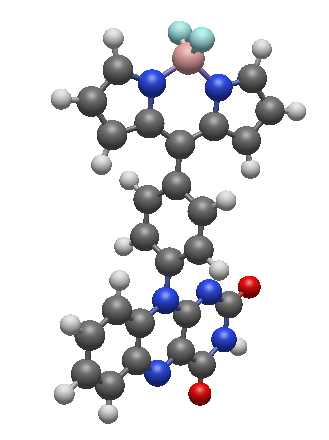
\includegraphics[width=0.9\textwidth]{Pics/FLVA.png}
%\captionof{figure}[This Figure]{Figure}
\end{minipage}
%\hspace{0.05\textwidth}
\begin{minipage}{0.45\textwidth}
\centering
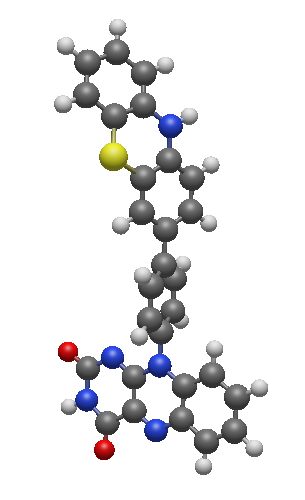
\includegraphics[width=0.9\textwidth]{Pics/DYAP.png}
%\captionof{figure}[This Figure]{Figure}
\end{minipage}
\caption{Molecular structure of borondipyrromethene-flavin (a) and phenothiazine-isoalloxazine (b)}
\label{fig:FLVADYAP}
\end{figure}

\subsection{Large Molecules: Challenges and Limitations}

An attempt was made to apply CDD-DF-SOS-ADC(2) to chemically interesting molecules with 5000 basis functions or more, with limited success: even if the atomic orbital formulation can exploit sparsity to reduce the memory footprint and scaling, the need for diffuse basis functions  practically nullifies any advantages it provides. The block occupation with aug-cc-pVDZ or def2-SVPD is still above 50\% for non-linear molecules with $\approx$ 300 atoms, and the very large auxiliary basis sets often lead to OOM (out-of-memory) errors due to data duplication in the QRDF algorithm and other routines. For diffuse auxiliary functions, processes often need to hold the whole $\cn{X}{Y}$ matrix in memory while solving the linear least squares problem. For multiple ranks on a single node, this can quickly lead to memory problems. While memory duplication can be reduced by simply using fewer ranks per node, it should be noted that currently the DBCSR tensor library is only optimized for one MPI rank per CPU. Furthermore, each rank can only allocate approximately 2GB of memory at once, because only 4-byte integers (with maximum value 2,147,483,648) are used to specify the size of the memory window that is allocated. Moreover, the need to reorder the tensors before each contraction effectively doubles the space needed by each tensor (see also the discussion in section \ref{sec:tenstor}).

In ground state methods, OOM errors can often be solved by using \emph{direct} methods where tensors are recomputed on-the-fly. By increasing the number of batches, the memory footprint can be lowered quite considerably. A direct version of CD-DF-SOS-ADC(2) could also be considered, although the need to recompute tensors like $C_{X\mu\nu}$, $R_{X\uli\olgn}$ or $B_{X\uli\olgn}$ multiple times would lead to a much higher prefactor which further pushes the low-scaling regime to larger molecular sizes.

\section{Summary and Outlook}

An atomic orbital formulation of the spin-opposite-scaled algebraic diagrammatic construction method can drastically reduce the formal quartic scaling of canonical, density-fitted SOS-ADC(2). This method, named CDD-DF-SOS-ADC(2), can successfully exploit the sparsity of the AO ground state density and the AO transition density. Furthermore, local density fitting significantly reduces the overhead, and the low scaling regime is more easily reached. For linear carboxylic acids, the method scales linearly, and even electron-dense systems, like hydrated formamide, were shown to have sub-cubic scaling if the transition density is sparse. The 3-index tensors necessary for a CDD-DF-SOS-ADC(2) calculation show a high degree of sparsity, which, when using block-sparse matrix storage, greatly reduces the memory footprint. Furthermore, the high prefactor of CDD-DF-SOS-ADC(2) can be mitigated using local density fitting, making it somewhat competitive with canonical density-fitted SOS-ADC(2) for dense systems, although with a much larger memory footprint.

Accuracy was shown to be within acceptable range for standard density fitting and quasi-robust density fitting. Convergence issues were encountered due to linear dependencies with the auxiliary basis sets, which can be addressed by removing certain basis functions, by canonical orthogonalization of the metric inverse, or by just using another basis set. 

Unfortunately, the need for augmented basis sets negatively impacts the scaling of CDD-DF-SOS-ADC(2) and delays the onset of the linear-scaling regime. Compared to NO methods, CDD-DF-SOS-ADC(2) includes all atomic orbitals and molecular orbitals, as opposed to only the ones close to the excitation region, making it more computationally expensive, although it has the advantage of not being state-specific. 

Pushing the current implementation of CDD-DF-SOS-ADC(2) to system sizes with a large number of basis functions ($>$ 5000 basis functions) quickly leads to memory problems, even on distributed systems. This, in combination with diffuse basis functions and molecular systems that are not strictly linear in nature, as well as the increased algebraic complexity of the working equations, means that CDD-DF-SOS-ADC(2) cannot really reach the low-scaling regime except in very specific cases. Introducing similar pre-screening techniques to NO methods based on some CIS or CIS(D) density might be beneficial. Moreover, a less memory-intensive tensor library should also be considered. However, at the moment, there are no other tensor libraries besides DBCSR that are well suited. Further development of sparse block tensor libraries are crucial for the future of atomic orbital based methods.

The equations for computing triplet excitations have not yet been implemented, but similar scaling and accuracy to singlet excitations are expected. 


\part{}

\chapter{Parallel Computing}

The popularity of computational chemistry can be attributed in no small part to the advances and development of highly efficient algorithms in theoretical chemistry. Equally important however is the ever increasing accessibility and performance of computing resources: commercially available work stations can handle chemical systems which could only be modeled on supercomputers a couple decades ago, and firmly cemented the position of computational chemistry as an important "experimental" tool in the toolbox of a chemist. 

As the speed of computers increased over the years, so did the complexity of their components. Nowadays, programmers can choose between several types of architectures, such as shared or distributed memory systems, or accelerators like GPUs. Knowing the strengths and weaknesses of each type is paramount to developing efficient algorithms and tackling larger molecular systems.

This chapter gives an overview on computer architecture, and the different types of parallelism encountered on modern hardware.

\section{Moore's Law}

\emph{Moore's Law} states that the transistor density in integrated chips doubles every 12 to 24 months. First formulated in 1965 by Gordon More, his prediction has held up fairly well over the years. However, the technology enabling this trend has changed over the years.

Figure \ref{fig:MOORE} shows the trends in clock speed, single-thread performance, power consumption and number of logical cores and transistors for microprocessors from 1970 to 2000. Since the early 2000s, clock-speed and single-thread performance have begun to plateau, and have stagnated from 2010 onwards. Increasing the clock speed to values beyond 4 to 5 GHz generates too much stress on the microchip in form of heat, and decreases its performance. This flaw was compensated by using the growing transistor density to instead increase the number of logical cores on a single chip. 

Shifting towards increasing core count however entails that the ideal performance for a CPU can only be achieved though parallel programming. Over the years, the number of different parallel hardware features has drastically increased, and it can be difficult for programmers to fully exploit the available computing resources. Moreover, different programming languages and compiler extensions have emerged as well, with numerous competing standards, especially for GPUs. 

\begin{figure}
\centering
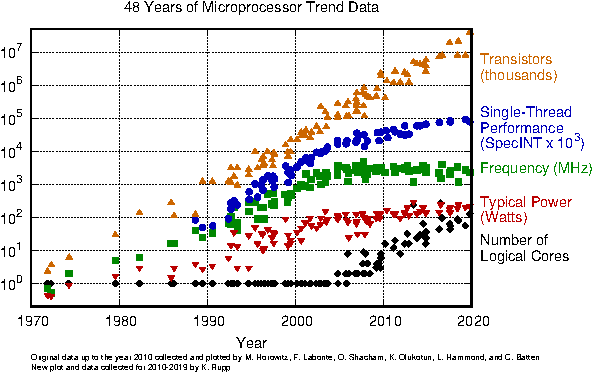
\includegraphics[scale=1.2]{Pics/moore}
\caption[Moore's Law]{Taken from \protect\url{https://github.com/karlrupp/microprocessor-trend-data}}
\label{fig:MOORE}
\end{figure}

\section{Benefits and Limits of Parallel Computing}

While the different available programming models can seem daunting at first, one of the major advantages of parallel computing is improved \emph{scalabilty}. An application that exposes parallelism can be sped up by several orders of magnitude, simply by adding more computing power, with several different architectures to choose from. The limit of what problem sizes can be tackled is mostly dictated by the \emph{amount} of available computing resources and storage, rather than individual processor characteristics.

As important as parallel computing has become in recent years, there is a reason why increasing clock speed was seen as the foremost strategy in keeping Moore's law alive. First, modifying a serial program to exploit parallelism can be a time-consuming endeavor, and second, not all tasks can be effectively parallelized. This means that the potential amount of seed-up is limited by the amount of parallel code. This is known as \emph{Amdahl's law}. The speed-up for a number of cores $N_c$ is given by
\begin{equation}
Speed-Up(N_c) = \frac{1}{S + \frac{P}{N_c}}
\end{equation}
\noindent where $S$ is the fraction of serial code and $P$ is the fraction of parallel code. The speedup for a fixed-size problem as a number of cores is known as \emph{strong scaling}, and the time-to-solution on each individual core \emph{decreases} when more cores are added.

An alternate way to compute potential speed-up is given by Gustafson-Barsis's Law
\begin{equation}
Speed-Up(N_c) = N_c - S(N_c-1)
\end{equation}
\noindent where the problem size also increases proportionally to the number of cores. The scaling for this trend is known as \emph{weak scaling}. In this scenario, the time-to-solution spend on each core remains constant, as the system size and number of cores increases. Even if this type is called "weak", both forms of scaling are equally important, as they address different scenarios. 

\section{Types of Parallelism and Memory Hierarchy}

Nowadays, a programmer has access to four categories of parallelism:
\begin{enumerate}
\item vectorization
\item thread-based parallelism
\item process-based parallelism
\item streaming
\end{enumerate} 
\noindent Leveraging the power of each type requires some understanding of the underlying hardware. 

Figure \ref{clusterArchitecture} shows the major components and memory pathways in a modern computing cluster. A \emph{cluster} is a collection of individual computers that work together and form a single unit. Individual computers are also called \emph{nodes} and occupy a single rack (or "shelf") each in a large server cabinet. The nodes are connected via a low-latency, high through-put network, e.g. Ethernet cables to enable inter-node communication. Each node contains one or more central processing units (CPU) and optionally one or more graphical processing units (GPU). Systems where different types of hardware architecture are mixed are also known as \emph{heterogeneous} systems. The individual components are fixed on a \emph{motherboard}: CPUs are plugged into \emph{sockets} and GPUs into \emph{PCIe slots}. A CPU is composed of one or more cores, where the actual processing of data is carried out. A GPU is also composed of multiple cores, which are grouped into independent \emph{streaming multiprocessors} (SM, NVIDIA), also known as compute units (CU, OpenCL), or subslices (Intel). 

\begin{figure}
\centering
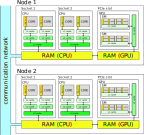
\includegraphics[scale=1.0]{Pics/memory}
\caption{Schematic representation of the architecture of a modern computing cluster which supports heterogeneous computing.}
\label{clusterArchitecture}
\end{figure}

Memory is also a crucial component of computer architecture and is a limited resource. The speed at which data is read from memory can also become a major bottle-neck: No matter how fast a processor is, if the feed rate is too low, it cannot reach its peak performance because it wastes cycles while waiting for data to arrive. To optimize data through-put, the memory model in modern computer architecture requires a complex hierarchy, with different sizes and speeds. Computer memory at the top of the hierarchy has a high response rate, but low complexity. It is also very expensive to produce and therefore much smaller. At the bottom of the hierarchy is memory with large storage space and capable of complex tasks. It is cheap but has low response rate. Over the years, the number of levels in the memory hierarchy has increased. Most modern computers have six levels: CPU registers, L1 cache, L2 cache, L3 cache, DRAM and disk. 

CPU registers sit at the top of the hierarchy and are closest to the cores. It is the region of memory where data is directly manipulated by arithmetic operations and machine code. Its size is typically on the order of several tens to hundreds of bytes. Data is loaded into the registers from \emph{cache}, a region of memory which is further subdivided into different levels named L1, L2 and L3. Each core has its own L1 cache, but might share L2 and L3 cache with other cores. Caches have different sizes and speeds, with L1 being the fastest and smallest at several tens of kB, and L3 being the slowest and largest at several tens to hundreds of kB. Memory is transferred from L3, to L2, to L1 and finally to the CPU registry. The reason why there are multiple levels of cache is to reduce \emph{cache misses}. If data requested by the core is not found in L1, then L2 is searched, then L3. A cache miss is an event where the data is not found anywhere in cache. In that case, a request has to be put out to the dynamical random access memory (DRAM) to retrieve data. Modern techniques such as \emph{cache prefetching} can minimize the amount of cache misses by loading the data into higher cache levels before it is actually needed by the lower levels. 

The speed of DRAM is 10 to 100 time slower than cache, but much larger in size. It is the main memory pool and shared by all cores. CPUs and GPUs have separate DRAM regions which communicate via a PCIe bus. DRAM sizes vary drastically, and are on the order of 10$^0$ to 10$^1$ for GPUs and 10$^0$ to 10$^3$ for CPUs. Data can be transferred from one node to another via CPU DRAM through the communication network, with transfer rates on the order of several GB/s. For programs which are not reading from disk, this is weakest link in the memory hierarchy ???

\section{Vectorization}

Vectorization is the process of operating on multiple variables at the same type. This type of parallelism is encountered at the highest level of the memory hierarchy introduced in the previous section, i.e. CPU registers. Each core has multiple registers, also called \emph{vector registers} with a certain size or \emph{vector length}. Instead of loading each individual element from cache and operating on it, one vector operation on a range of elements can replace multiple single operations. For a 512-bit register, two vectors with 8 floats (32 bit) can be summed within one cycle instead of eight. This type of parallelism is also known as single instruction multiple data (SIMD) in \emph{Flynn's taxonomy}.

The length of vector registers, number of registers as well as the number of supported vector operations have greatly expanded over the years (Table \ref{VECTORHARDWARE}).

\begin{table}
\makegapedcells
\centering
\begin{tabular}{p{0.3\linewidth}cc}
\hline
Release & Vector Length (bit) & No. Registers \\ \hline
SSE (Streaming SIMD Extension) & 128 & 8 \\ 
SSE2/SSE3/SSE4 & 128 & 16  \\
AVX/AVX2 (advanced vector instructions) & 256 & 16 \\
AVX512 & 512 & 32 \\ 
\hline 
\end{tabular}
\caption{Vector lengths and number of registers for commonly encountered vector extensions.}
\label{VECTORHARDWARE}
\end{table}

\subsection{Parallel SAXPY using vectorization}

To show how vectorization can be used in a program, consider the following vector operation:
\begin{equation}
y \leftarrow \alpha x + y
\label{DAXPY}
\end{equation}
\noindent where $y$, $x$ are vectors of equal length, and $\alpha$ is a scaling factor. The vector operation \ref{DAXPY} is also known as "saxpy" for single precision, and "daxpy" for double precision. A naive implementation of the saxpy-kernel is given in Listing \ref{lst:SAXPYNOPARA} for vector size $N$  

\cppcode{Parallelization-unaware implementation of saxpy \label{lst:SAXPYNOPARA}}{listings/saxpy_nopara.c}

\noindent Two arrays are allocated, x and y, and all their entries set to 1 and 2 respectively. Each element is updated individually in the for loop. There are several possibilities to introduce vectorization:
\begin{enumerate}
\item auto-vectorization
\item compiler directives
\item intrinsic functions
\item optimized libraries
\end{enumerate}
\noindent Auto-vectorization is by far the easiest approach: the compiler automatically recognizes that the loop can be vectorized and generates optimized machine code that uses vector instructions. This does not require any input from the user. Compiling the code on a machine with AVX support, using the GNU C compiler, and passing the compiler flags "-O2 -march=native -ftree-vectorize -fopt-info-vec-optimized" generates the following report:
\begin{lstlisting}[backgroundcolor=\color{light-gray},breaklines=true]
saxpy_nopara.c:9:3: optimized: loop vectorized using 32 byte vectors
\end{lstlisting}
\noindent which indicates that the vectors are loaded and operated on in 32 byte chunks, or 8 floats at once. The flag "-ftree-vectorize" (or alternatively "-O3") activates auto-vectorization and "-fopt-info-vec" generates the report. To make sure that the C compiler uses the right vectorization release, the flag "-march=native" is needed, or else the compiler might fall back to SSE. 

In some cases, auto-vectorization cannot take place because the compiler did not recognize that the loop can be vectorized. It can then be beneficial to use \emph{intrinsic functions}. Intrinsic functions are compiler-dependent functions that map to processor operations. When targeting an AVX architecture with 256-bit registers, the saxpy kernel can be rewritten as
\cppcode{SAXPY using intrinsics \label{lst:SAXPYINTRINSICS}}{listings/saxpy_intrinsic.c}
\noindent It is apparent that using intrinsics makes the program much more complex. The arrays cannot be fed directly to the functions, but need to be loaded into vectors of type \texttt{\_\_mm256}, using "set" or "load" functions. Furthermore, the data needs to be aligned correctly using \texttt{\_\_attribute\_\_ ((aligned(...)))}. The arrays are then loaded in chunks into the registers and given to the vector functions for multiplying and adding. 

The major problem with using intrinsic functions, besides increased complexity, is \emph{portability}. The code in \ref{lst:SAXPYINTRINSICS} does not compile on machines that do not support AVX, and is limited to 256-bit registers even on AVX-512 machines. Portable alternatives include using compiler directives or optimized libraries.

Directives (or "pragmas") are hints that can be given to the compiler that suggest that the loop might be vectorizable. By far the most popular set of compiler directives that provide vectorization capabilities is undoubtedly included in the OpenMP application programming interface (API). The OpenMP API is standardized across all compilers, making it highly portable. The OpenMP directives greatly simplify the SAXPY program:
\cppcode{SAXPY using compiler directives \label{lst:SAXPYDIRECTIVES}}{listings/saxpy_simd.c}
\noindent Simply plopping the directive in front of the for loop takes care of generating the appropriate machine code for the targeted architecture. 

The last way to introduce vectorization is via external programs, such as the basic linear algebra subprograms (BLAS) library. It provides a set of specific functions for performing basic vector and matrix operations. Similar to OpenMP, it only provides specifications, and the direct implementation is compiler-dependent. In the BLAS routines, there is a saxpy functions available that can be called directly. It has the advantage of completely removing the loop and clearly states what operation is performed.
\cppcode{SAXPY using BLAS \label{lst:SAXPYBLAS}}{listings/saxpy_blas.c}
\noindent External libraries can however be associated with a steeper learning curve depending on the complexity of function signatures.

\section{Thread-based Parallelism}

Vectorization is limited to single cores only. For multi-core processing, it is important to understand the concept of processes and threads. Processes are executing instances of programs that group related operating system resources together. These resources are exclusive (private) to the process which allocated them, such as system memory, file handles, I/O status information, scheduling information and accounting information. 

A process spawns one or more \emph{threads} (Figure \ref{fig:shared}). A thread is the smallest subset of a process that can be scheduled independently by the OS scheduler. Unlike processes, threads of the same process share resources. They can be seen as "light-weight" processes: start-up of individual threads and communication between threads is much faster. Each core executes only  one thread at a time, but can quickly switch between different threads (or \emph{contexts}). Threads with a higher \emph{priority} are granted more CPU time than threads with lower priority. One a single-core processor, threads are only executed \emph{concurrently}, i.e. they are paused and resumed at regular intervals depending on their priority. On multi-core processors, threads can be executed at the same time (multi-threading), but concurrency is still needed if the number of threads exceeds the number of logical cores.

\begin{figure}[h]
\centering
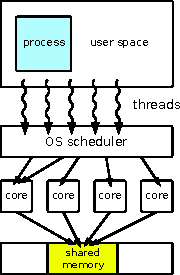
\includegraphics[scale=1.4]{Pics/shared}
\caption{Shared memory parallelism}
\label{fig:shared}
\end{figure}

\subsection{SAXPY using OpenMP}

The most popular standard for thread-based parallelism (or \emph{shared-memory parallelism}) is OpenMP, which was briefly discussed in the previous section. OpenMP was originally introduced to parallelize highly regular loops, but the standard has since then been greatly expanded and includes vectorization directives as well. Using pragmas, multiple threads can be spawned that execute the code within the parallel region. Listing \ref{lst:SAXPYOMP} shows an OpenMP parallel version of SAXPY. Each thread in the parallel region has a unique number associated with it which is used to divide up the arrays. Caution needs to be taken that threads do not operate on the same region at once, as this can lead to undefined behavior ("race conditions").  
\cppcode{SAXPY using OpenMP \label{lst:SAXPYOMP}}{listings/saxpy_omp.c}
\noindent Alternatively, the code may be more easily expressed by using a single compiler directive:
\cppcode{SAXPY using OpenMP \label{lst:SAXPYOMP2}}{listings/saxpy_omp2.c}
\noindent The \texttt{omp parallel for} directive also offers different scheduling tactics which may be difficult to program by hand. Listing \ref{lst:SAXPYOMP} is an example of \emph{static scheduling}, where the work is divided equally among threads \emph{a priori}. However, in the case where each step requires different computational cost, \emph{dynamic scheduling} offers a more balanced approach, although with a somewhat higher prefactor. Threads request tasks, or a chunk of multiple tasks, from the main thread, which distributes work on a first-come first-serve basis. There are many more directives available in the OpenMP standard with a lot of options for fine-tuning. For further details, the reader is referred to the official specifications \cite{OMP2021}.
% (ref) https://www.openmp.org/specifications/

OpenMP is not the only option available for introducing shared-memory parallelism into a program. Alternatives include the \texttt{pthread} (POSIX threads) library for C, the \texttt{std::thread} library, or the Intel TBB (thread building blocks) library for C++. While these libraries can offer a more fine-grained control of threads, the learning curve can be very steep, and parallelizing an application can be very time-consuming. In contrast to OpenMP, they are not based on high-level compiler directives, but rather expose low-level functions and structures that create and control threads. 

Shared-memory parallelism, as the name implies, is limited to cores sharing the same memory space. The primary disadvantage of this model is scalability. It becomes increasingly expensive to produce shared memory systems with more and more cores. Moreover, a larger number of cores implies heavier CPU traffic and time penalties due to \emph{cache coherence}. Cache coherence is the mechanism by which uniformity of data is guaranteed and propagated among processes. There can be multiple copies of the same memory region in cache, which is operated on by different cores. Checking how to combine data from different caches can become costly for a large number of cores.

\section{Process-based Parallelism}

One of the most scalable approaches in parallel computing is process-based parallelism, also known as distributed memory parallelism. Multiple copies of the same program run on separate processes, each with their own local memory and instruction set. In contrast to threads, processes cannot exchange data via shared memory, but need to communicate via a network using \emph{message passing}. The increased cost of communication is often outweighed by the increased potential for scalability. Larger problems can be tackled simply by adding more nodes. 

Pure message-passing assigns or \emph{binds} one rank to a single CPU core. In hybrid parallel approaches, a single process can be bound to a whole node, using shared-memory parallelism for intra-node communication and message passing for inter-node communication. It is also possible to spawn more processes than there are available cores: in that case, the processes are scheduled and executed concurrently similar to threads.

The most popular standard for message passing is the message passing interface (MPI). It defines a set of functions that allow processes to send and receive messages. There are different implementations of MPI, such as the open-source implementations OpenMPI, MPICH, or the vendor implementations Intel MPI or Cray MPI. MPI programs are run using a special start-up command:
\begin{lstlisting}[backgroundcolor=\color{light-gray},breaklines=true]
mpirun -n <nprocs> ./myprogram.exe 
\end{lstlisting}
\noindent The exact command and options depends on the MPI implementation. The start-up program is responsible for duplicating the program on the different processes and establishing the communication network. Most implementations use the flag \texttt{-n} to pass the number of processes to be spawned. 

All processes are characterized by their \emph{rank}, a unique, portable identifier, normally an integer between $[0:nprocs-1]$. Only processes using the same \emph{communicator} can exchange messages. A communicator is a special handle of type \texttt{MPI{\_}Comm} and describes a group of processes. Communicators may also have different \emph{topologies}, such as Cartesian grids, or  graphs, which restrict the flow communication between processes to nearest neighbors. Cartesian grids for example are best suited for matrix operations. By passing topology information to MPI, it can optimize the runtime environment by renumbering tasks such that processes are physically closer to reduce communication overhead. By default, the topology is undefined, and any processor can exchange messages with all other processors.

\subsection{SAXPY using MPI}

Modifying programs to exploit distributed parallelism requires significant effort, with the most crucial point being how data is distributed over the processes. Consider again the SAXPY kernel. There are two memory models: either every process has a copy of the whole array, or the arrays are distributed in chunks over all processes. If data is duplicated on every rank, this can quickly exhaust memory resources for large data sets. On the other hand, if data is distributed in a non-ideal way, commutation may incur major overhead. A programmer has to balance the benefits of data duplication and network communication. 

Listing \ref{lst:SAXPYMPI} shows a distributed memory approach to the SAXPY kernel
\cppcode{SAXPY using MPI \label{lst:SAXPYMPI}}{listings/saxpy_mpi.c}
\noindent The program starts by initializing the executing environment using \texttt{MPI{\_}Init}, and defining the communicator handle. The communicator that groups all processes at start-up is called \texttt{MPI{\_}COMM{\_}WORLD}, and is a macro defined in the header \texttt{<mpi.h>}. If the program is stand-alone, it is safe to use as the primary communicator. When writing a library that is used in combination with other MPI libraries, it is crucial to use a communicator that is passed from the main program. There are two reasons for this: (1) the user may want to use a subcommunicator, rather than the whole process group, and (2) MPI messages have a unique identifier (integer) and if another library uses the same identifier, erroneous communication can take place. In this example, the global communicator is sufficient.

Each process then allocates a local array of size \texttt{num{\_}local} $<$ \texttt{ARRAY{\_}SIZE}. In this example, the main data is initialized on rank 0, which is then split into equal chunks and send to the other processes' local array using \texttt{MPI{\_}Scatter}. Each process then only needs to perform the SAXPY operation on its local chunk. Afterwards, the results are collected on rank 0 using the routine \texttt{MPI{\_}Gather}. Data is then available on rank 0 to be further manipulated, written to console, etc. 

It should be noted that the above program only works for a number of processes that is a divisor of \texttt{ARRAY{\_}SIZE}, because \texttt{MPI{\_}Scatter} and \texttt{MPI{\_}Gather} can only handle chunks that are of equal size on each process. If that is not the case, one can use the more general routines \texttt{MPI{\_}Scatterv} and \texttt{MPI{\_}Gatherv} which also take the different chunk sizes as an input.

Furthermore, the local SAXPY for-loop can be parallelized using the techniques described in the previous sections (vectorization, threads) in case where a process is bound to a whole node and has access to further compute resources.

This program shows only a few of the many functions available for message passing. The MPI standard defines many more functions for sending, receiving, broadcasting, reduction, one-sided communication etc. The official document for the newest MPI standard \cite{MPI2021} is over a thousand pages long, and is updated regularly. Message passing has a very steep learning curve, and can be quite difficult to debug.  

% ref https://www.mpi-forum.org/docs/

\subsection{MPI and Shared Memory}

One may come under the impression that MPI is not efficient on shared-memory systems, as data is exchanged via network-calls. However, MPI is optimized to recognize shared memory and data is then copied within DRAM rather than send through a communication layer, making MPI competitive even on single nodes. Of course, there is still a slight overhead associated with it compared to thread-based parallelism.

MPI standards of version 3.0 and above furthermore introduce functions to allocate shared memory, also known as \emph{windows}, for processes on the same node. Processes can then read/write to the same memory region without using network calls, much in the same manner as OpenMP. This approach can be seen as a MPI+MPI hybrid parallel approach rather than the more frequently used MPI+OpenMP approach. Hybrid parallelism is much more efficient than "MPI-everywhere" approaches due to reduced communication overhead and easier load-balancing. 

MPI+MPI has the advantage of only needing one programming model for both distributed and shared memory access, with relatively easy syntax. However, MPI+MPI is much lesser known, and there are is no automatic support for splitting up loops or atomic loads/stores to shared memory. An external library that offers auxiliary functions for MPI+MPI would be beneficial.

\section{Stream Processing}

The last type of parallelism tackled in this chapter is \emph{stream processing}. A stream is defined as a sequence of data that requires similar (low-level) computation. Streams are processed by \emph{accelerators}, special hardware components with high data throughput, that complement the general purpose CPU by speeding up certain operations. 

\subsection{GPU Architecture}

By far the most popular type of accelerators are graphical processing units (GPUs). As the name implies, GPUs were originally conceived to speed up graphics-related computation, but their use was later extended to include non-graphics workloads as well, in what is known as \emph{general-purpose} graphic processing unit (GPGPU) programming. Nowadays, computing clusters increasingly come with one or more GPGPUs included on each node.

The hardware architecture design of modern GPUs is much more varied than that of CPUs. GPU vendors, like NVIDIA or AMD, have different hardware variations and use different terminology for similar components, and it can be difficult to abstract hardware as some vendor-specific features need to be omitted. Figure \ref{fig:gpu} shows a simplified block diagram of the most common GPU components. A GPU is composed of multiple compute units (CUs), also known as streaming multi-processors (SMs) in NVIDIA GPUs. Work is assigned to different CUs by a workload distributor. Each CU is further subdivided into an array of processing elements (PEs), or CUDA cores as referred to by NVIDIA. A single PE can operate on multiple data elements at once using SIMD or a variation known as single instruction multiple threads (SIMT) used in CUDA cores.

The overall performance of a GPU is given by the number of CUs and PEs, as well as the bandwidth of the PCIe land connecting CPU and GPU. Data transfer between the two devices is often the time-determining step.

\begin{figure}
\centering
\includegraphics[scale=2.0]{Pics/gpu}
\caption{GPU architecture}
\label{fig:gpu}
\end{figure}

\subsection{GPU Programming Model}

The rise of GPGPU programming has given rise to a plethora of different programming languages and models. Low-level languages like CUDA, OpenCL or HIP directly reflect features of the targeted GPU hardware as part of their syntax, and the user is responsible for managing each aspect of parallelism and data transfer. They require a very thorough understanding of how GPUs operate. Due to the complexity of "native" languages, higher-level languages have gained popularity over the years. Pragma based languages like OpenACC or OpenMP offer a much easier approach to GPU programming that resembles shared memory parallelism on CPUs, and offer a higher degree of portability, at the cost of lower performance ceiling.

Low level languages all operate on a similar programming model which allow the programmer to define special functions called \emph{kernels}, which, when called on a GPU, are executed $N$ times in parallel by $N$ GPU threads. Rather than using for loops, kernels operate on a whole range of data at once, known as a \emph{grid} or NDRange. A grid can be one, two or three-dimensional to allow a more intuitive view of the data at hand. Each grid is subdivided into blocks or work groups which can be executed independently. The maximum size of a block is given by the number of threads in a CU. "Good" values are generally 128, 256 or 512, but the optimal size depends on the hardware and the problem addressed. Threads in a block share memory which is useful in case data from neighboring subblocks is needed. Information on grid and block dimensions are needed by the kernels for distributing work over the GPU.

As an example, consider the SAXPY function using the CUDA programming language:
\cppcode{SAXPY using CUDA \label{lst:SAXPYCUDA}}{listings/saxpy_cuda.cu}
\noindent CPU and GPU do not share memory. The first steps therefore involve allocating memory using \texttt{cudaMalloc} and copying data from CPU ("Host") to GPU ("Device") with the function \texttt{cudaMemcpy}. The arrays can then be passed to the kernel. The kernel function is indicated by the identifier \texttt{\_\_ global\_\_}, and is executed at the same time by all threads in a block. Each thread has a unique block and thread id which indicate its position in the work group. This information is used to make sure that the thread is operating on the correct portion of the array. The GPU threads do not have any information of the loop extent, and it is the user's responsibility to make sure that threads do not write past the allocated memory window by introducing boundary checks (\texttt{if (i < N)}).

In this example for a 1D array, the kernel takes two launch parameters: the number of blocks, and the block size which are put between \texttt{<<< .... >>>} after the function call. Afterwards, the data can be copied back to the CPU for further processing. 

The concept of operating relative to thread coordinates rather than using a for loop with a single index can be quite confusing. Nowadays, there are directive-based compiler extensions, that allow to easily offload work to accelerators, such as OpenMP and OpenACC (Open ACCelerators). Listing \ref{lst:SAXPYACC} shows how a for loop can be easily modified using OpenACC
\cppcode{SAXPY using OpenACC \label{lst:SAXPYACC}}{listings/saxpy_acc.c}
\noindent OpenACC offers several pragmas for allocating and copying arrays to GPUs and back. By only adding two directives, the SAXPY code is easily ported to GPUs. 

\subsection{When to Use GPUs}

Despite the success of GPU computing, GPUs only complement, rather than replace CPUs. GPU cores are very light-weight and have a limited instruction set compared to CPU cores, making them ill-suited for \emph{task-based parallelism}, e.g. running an operating system with many different processes executing in the background. The strength of GPUs rather lies in \emph{data-based parallelism}. Generally, any code that can benefit from vectorization can be sped up using GPUs. 


\chapter{Into The Matrix}

At its core, computational chemistry is basically matrix algebra applied to molecular systems. The performance of an algorithm, in other words its scaling, memory footprint and even accuracy, is intimately linked to how matrix operations and storage are handled internally. While the earliest implementations of molecular electronic structure methods often used hand-coded loops running over matrix indices, over the years, a whole ecosystem of matrix and tensor libraries has emerged in an attempt to lessen the burden of programmers, to various degrees of success, each with their strong and weak points. Choosing the best library for an algorithm is a non-trivial task, and depends on various factors: if memory is the bottle-neck, a sparse matrix library might be able to sufficiently compress data into a smaller space. If speed is the greatest concern, targeting different architectures like distributed memory systems, accelerators, or both, might be the solution.

This chapter introduces basic concepts of matrix and tensor algebra, with a focus on storage orders. After introducing the core concepts, a small list of matrix libraries used in \mchem{} is provided which summarizes the core functionalities.

\section{Linear Algebra}

Linear algebra is a crucial tool in many areas of computational science, such as image processing, machine learning, computational physics, computational biology and of course computational chemistry. The most important concepts are discussed in this section. Until mentioned otherwise, zero-based indexing is assumed. 

\subsection{Matrices}

A matrix is a rectangular, 2-dimensional array of dimension $M$ by $N$, containing a set of complex or real numbers $\{a_{ij}\}$ with ordered subscripts $i = 0,1,2,...M$ and $j = 0,1,2,...,N$, of the form
\begin{equation}
\mbf{A} = \begin{pmatrix}
a_{00} & a_{01} & \ldots & a_{0N} \\
a_{10} & a_{11} & \ldots & a_{1N} \\
\vdots & \vdots & \ddots & \vdots \\
a_{M0} & a_{M1} & \ldots & a_{MN}
\end{pmatrix}
\end{equation}
\noindent with $M$ \emph{rows} and $N$ \emph{columns}. \emph{Row vectors} and \emph{column vectors} are types of matrices that contain only one row or one column, respectively. 

Matrix multiplication is only defined between matrices of dimension $M$ by $K$ and $K$ by $N$. The product yields an $M$ by $N$ matrix
\begin{align}
\mbf{C}_{M\times N} &= \mbf{A}_{M\times K} \mbf{B}_{K\times N} \\
c_{ij} &= \sum_k a_{ik} b_{kj}
\end{align}

A matrix with an equal number of rows and columns is called a \emph{square matrix}. There a different types of square matrices:
\begin{enumerate}
\item \emph{Diagonal matrices} only have non-zero entries on the diagonal
\begin{equation}
a_{ij} = a_{ii} \delta_{ij}
\end{equation}

\item If all entries below the diagonal are zero, the matrix is \emph{lower triangular}. Similarly, if all elements above the diagonal are zero, the matrix is \emph{upper triangular}. Furthermore, if the diagonal entries are all equal to 1, the matrix is \emph{unit triangular}.

\item The \emph{identity} or \emph{unit} matrix $\mbf{1}$ is defined as
\begin{align}
\mbf{A} \mbf{1} &= \mbf{1} \mbf{A} \\
\mbf{1}_{ij} &= \delta_{ij}
\end{align} 

\item The \emph{inverse} of a matrix $\mbf{A}$ is defined as
\begin{equation}
\mbf{A}^{-1} \mbf{A} = \mbf{1}
\end{equation} 
\noindent It only exists for matrices with a non-zero determinant. If a matrix is non-invertible, it is also called \emph{singular}. 

\item A matrix is \emph{unitary}, if its inverse is equal to its conjugate transpose 
\begin{equation}
\mbf{A}^{-1} = \mbf{A}\pdg
\end{equation}
\noindent A real unitary matrix is called \emph{orthogonal}

\item A \emph{hermitian} matrix is its own conjugate transpose
\begin{align}
\mbf{A} &= \mbf{A}\pdg \\
a_{ij} &= (a_{ji})^*
\end{align}
\noindent A real hermitian matrix is called \emph{symmetric}

\item A hermitian matrix is said to be \emph{positive definite} if all of its eigenvalues are positive, and \emph{negative definite} if all eigenvalues are negative. \emph{Semi-definite} matrices additionally have some eigenvalues which are equal to zero.   
\end{enumerate}

%\subsection{Matrix Decompositions}
%
%Matrix decomposition (or factorization) is one of the fundamental disciplines in linear algebra. Decompositions reduce a matrix into a product of matrices. They can be used to solve a system of linear equations, solve the linear least squares problem, invert a matrix, analyze the numerical stability of a system, or find the \emph{rank} of a matrix, i.e. the number of linearly independent column vectors. Some decomposition techniques can factorize a large and complex matrix into smaller constituents that are more easy to operate on. Examples of matrix decomposition algorithms include
%\begin{enumerate}
%
%\item The \emph{eigenvalue decomposition} finds a transformation matrix $\mbf{V}$ such that it diagonalizes the matrix
%\begin{equation}
%\mbf{A} = \mbf{V} \boldsymbol{\Lambda} \mbf{V}^{-1}
%\end{equation}
%\noindent where $\boldsymbol{\Lambda}$ is a diagonal matrix containing the eigenvalues. This decomposition is only possible for square matrices.
%
%\item The \emph{LU} factorizes a symmetric matrix into a product of a lower triangular matrix $\mbf{L}$ with its transpose
%
%\end{enumerate}

\section{Matrix Storage Formats}

The main memory in a computer, i.e. DRAM, is a linear address space and can be seen as a single, contiguous, one-dimensional array. Two-dimensional arrays like matrices need to be \emph{mapped} to this linear space by the compiler. This mapping depends on whether a dense or sparse view of the matrix is desired. 

\subsection{Dense Storage}

There are two ways to map a dense matrix to memory: row-major ordering and column-major ordering. The two storage orders differ by the order in which the individual elements are stored in memory. For an $M$ by $N$ matrix stored in a linear array $a$ in row-major format, the address offset of an element $a_{ij}$ compared to element $a_{00}$ is given by
\begin{equation}
A(i,j) \rightarrow \text{a[i * N + j]}
\end{equation}
\noindent and in column-major format by
\begin{equation}
A(i,j) \rightarrow \text{a[i + j * M]}
\end{equation}
Neither storage order has any advantages or disadvantages over the other one. It is only a matter of convention, and depends on the library and programming language. Fortran arrays are column-major, while C/C++ arrays are row-major. 

However, algorithms optimized for column-major access might not give the same performance for row-major formats and vice-versa. Consider a simple loop over matrix elements in the Fortran programming language
\begin{fortran}{Matrix Loop \label{FORTRAN1}}
DO i = 1, N
 DO j = 1, N
  A(i,j) = A(i,j) + 2
 ENDDO
ENDDO
\end{fortran}
\noindent By first looping over the rows, and then over the columns, the elements in the column-major matrix are accessed in a \emph{non-contiguous} manner. This prevents efficient optimizations like vectorization due to cache misses. By swapping the loops, the inner loop can be vectorized. Therefore, if algorithms assume a certain ordering, it is important to pass matrices of the same ordering.

Column-major ordering is by far the most common in scientific computing. Matrix algebra routines like the QR, Eigenvalue or Cholesky decompositions are most intuitively written using column operations rather than row operations. Examples include the LAPACK and Eigen matrix libraries. 

\subsection{Sparse Storage}

A matrix is called \emph{sparse} if "most" of its elements are zero. The threshold between sparse and dense is ill-defined, and range anywhere between 1\% and 10\%. Sparse matrices are encountered in many fields of computational science in systems with few pair-wise interactions. By storing and looping over the significant elements only, the memory footprint and the scaling of matrix multiplications or decompositions can be significantly reduced. There are several different sparse matrix formats available. The following sections will demonstrate how the matrix
\begin{equation*}
\begin{pmatrix}
3 & 5 & 0 & 0 \\
0 & 4 & 0 & 0 \\
0 & 0 & 1 & 2 \\
0 & 0 & 6 & 7 
\end{pmatrix}
\end{equation*}
\noindent may be represented using some of these formats.

\subsubsection{Coordinate Format}

The coordinate format (COO) is one of the simplest storage schemes for sparse matrices. The matrix is stored using three arrays of length $NNZ$ (number of non-zero elements) containing the row indices, column indices and matrix entries. The above matrix reduces to 
\begin{equation*}
COO: \left\lbrace
\begin{matrix}
\textrm{idx\_i} &= &\left[ 0, 0, 1, 2, 3, 2, 3 \right] \\
\textrm{idx\_j} &= &\left[ 0, 1, 1, 2, 2, 3, 3 \right] \\
\textrm{val}   &= &\left[ 3, 5, 4, 1, 6, 2, 7 \right] \\
\end{matrix}
\right.
\end{equation*}
\noindent The values do not need to be necessarily ordered. The COO format has the advantage that it is very easy to insert elements and change the sparsity pattern with low overhead. COO is generally not used for algebra due to slow random access of elements if they are not stored in order. Rather, COO is an intermediate format for incremental construction of sparse matrices in the CSR or CSC format.

\subsubsection{Compressed Sparse Row}

The compressed sparse row format (CSR) is similar to COO, but compresses the rows. A CSR matrix is represented by three arrays: the extent of rows, the column indices and non-zero matrix entries, with dimension $M$, $NNZ$ and $NNZ$ respectively. For the example matrix above, the CSR format gives
\begin{equation*}
CSR: \left\lbrace
\begin{array}{lll}
\textrm{row\_ext} &= &\left[ 0, 2, 3, 5 \right] \\
\textrm{col\_idx} &= &\left[ 0, 1, 1, 2, 2, 3, 3 \right] \\
\textrm{val}  &= &\left[ 3, 5, 4, 1, 2, 6, 7 \right] \\
\end{array}
\right.
\end{equation*}
\noindent The $i$th entry of the row extents contains the offset to the first non-zero element in the array \textrm{val} in the $i$th row. The entries in \textrm{col\_idx} are the associated column indices. Compared to COO, accessing elements is much faster, and the memory prefactor is reduced from $3NNZ$ to $2NNZE+M$. Matrix-vector products are very fast to compute, but CSR in not well suited for column slicing.

\subsubsection{Compressed Sparse Column}

The compressed sparse column format (CSC) is the "column-major" analog to the CSR format. Instead of compressing the rows, it compresses the columns. The matrix in the CSC format is represented as

\begin{equation*}
CSC: \left\lbrace
\begin{array}{lll}
\textrm{col\_ext} &= &\left[ 0, 1, 3, 5 \right] \\
\textrm{row\_idx} &= &\left[ 0, 0, 1, 2, 2, 3, 3 \right] \\
\textrm{val}  &= &\left[ 3, 5, 4, 1, 6, 2, 7 \right] \\
\end{array}
\right.
\end{equation*}

CSC has similar performance to CSR, but is better suited for column slicing and therefore column-oriented matrix decomposition.

\subsection{Block Compressed Sparse Row}

The block-compressed sparse row (BCSR or BSR) format is a generalization of CSR. BCSR is ideal for matrices which are \emph{block-sparse}, i.e. matrices with few dense submatrices. For a constant block size $n$ by $m$, let the number of row and column blocks be $M_{blk}$ and $N_{blk}$, and $NNZ_{blk}$ the number of significant blocks. A matrix is then represented by three arrays containing the row block offsets, column block indices, and non-zero indices with size $M_{blk}$, $NNZ_{blk}$ and $NNZ_{blk}mn$. For blocks of size 2 by 2, the matrix above in the BCSR format yields

\begin{equation*}
BCSR: \left\lbrace
\begin{array}{lll}
\textrm{rowblk\_ext} &= &\left[ 0, 1 \right] \\
\textrm{colblk\_idx} &= &\left[ 0, 1 \right] \\
\textrm{val}  &= &\left[ 3, 0, 5, 4, 1, 6, 2, 7 \right] \\
\end{array}
\right.
\end{equation*}

\noindent The matrix is therefore split into two non-zero blocks of size 2-by-2 each, with elements $\{3,0,5,4\}$ and $\{1,6,2,7\}$ using column-major ordering. The BCSR format can further reduce the storage prefactor for block-sparse matrices compared to CSR or CSC. Smaller block-sizes can account for a higher degree of sparsity, but lead to a higher prefactor. Large block sizes have lower prefactor, but capture less of the sparsity. Figure \ref{fig:DISTSTOR2} shows the BCSR format for different split factors. The block sizes do not need to be the same, although a constant block size is best suited for load balancing. Whether a block is significant or not depends on the matrix norm that is chosen as a criterion for filtering. Popular choices include the Frobenius norm or the max norm. 

\subsection{Distributed Storage}

In distributed memory parallelism, processes do no longer have access to the whole matrix. The question then arises how to distribute data over multiple nodes or processes. Distribution can be \emph{blocked} or \emph{cyclic} (Figure \ref{fig:DISTSTOR1}). In the block representation, the matrix is distributed by dividing rows, columns (or both) by the number of processes, and distributing them sequentially over the processes. On the other hand, the cyclic representation distributes each individual row, column or matrix element over the set of processes and wrapping over them until all elements are assigned to a processor. The cyclic data layout achieves great load balancing by evenly distributing the matrix elements, but is not suitable for row or column manipulations due to a high communication overhead. A blocked representation can reduce this overhead, but load-balancing is more difficult to achieve if the number of elements is not evenly divisible by the number of processes. 

The most commonly used format for distributed matrix storage is the \emph{block-cyclic} representation (Figure \ref{fig:DISTSTOR2}). It combines the best of both worlds, with good load-balancing and low communication overhead for matrix algebra. Communication is most efficient by arranging processes into a 2-dimensional rectangular grid with $N_{proc} = N_{row} \times N_{col}$, such that each process is uniquely identified by its coordinates $(i,j)$. A 4-by-2 grid therefore has 4 \emph{process rows} and 2 \emph{process columns}. With MPI, this is most easily achieved by using \emph{Cartesian grids}. In Cartesian grids, processes can only communicate with their nearest neighbor. Each process has a local array which can be packed in different ways. While the ScaLAPACK library keeps the original ordering of the matrix elements, other matrix libraries like DBCSR store the individual blocks sequentially in memory. Blocks do not necessarily need to be equal in size. Libraries like DBCSR also support heterogeneous block sizes.

All the sparse storage schemes discussed in the previous sections can also be applied to distributed matrices. DBCSR uses a block-sparse row format which distributes the significant blocks over the processors in a row-major format (Figure \ref{fig:DISTSTOR3}). 

\begin{figure}
\centering
\includegraphics[scale=0.25]{Pics/DISTSTOR1.pdf}
\caption[Cyclic and blocked distribution]{There are two distinct ways to distribute rows, column or elements along processes, namely cyclic and block. Each color represents a processor (4 in total).}
\label{fig:DISTSTOR1}
\end{figure}

\begin{figure}
\centering
\includegraphics[scale=0.25]{Pics/DISTSTOR2.pdf}
\caption[Block-cyclic distribution]{In the block-cyclic distribution, the matrix is divided into blocks which are distributed over a processor grid, in this case 2 $\times$ 2.}
\label{fig:DISTSTOR2}
\end{figure}

\begin{figure}
\centering
\includegraphics[scale=0.25]{Pics/DISTSTOR3.pdf}
\caption[Distributed block compressed sparse row format]{The DBCSR library distributes the significant blocks over the processor grid in row-major format.}
\label{fig:DISTSTOR3}
\end{figure}

%¨libxsmm?
%The block size has a major impact on the performance of distributed linear algebra algorithms. Consider the multiplication of two matrices. Multiplication can be reformulated in terms of individual multiplications of sub-blocks. 

\section{Tensors}

\subsection{Definitions}

Tensors are multi-dimensional arrays and can be seen as a generalization of matrix objects to higher dimensions, containing a set of complex or real values $\{a_{ijk...}\}$ with the ordered indices $i = 0,1,2,...N_0$, $j = 0,1,2,...N_1$, $k = 0,1,2,...N_2$ etc. The total number of indices required to identify an element in a tensor corresponds to its \emph{dimension}, also called \emph{rank}, \emph{order} or \emph{degree}. It should be stressed that tensor rank is different from the concept of a matrix rank. 

Tensors are important quantities in various scientific fields, especially in physics and quantum chemistry. Examples of tensor are the 4-dimensional MP2-amplitudes $t_{iajb}$ or the 3-dimensional 3c2e electron integrals. Matrices can be seen as 2-dimensional tensors. 

The analog of matrix multiplication is \emph{tensor contraction}, which involves the summation over one or multiple indices. Consider for example the tensor contraction
\begin{equation}
C_{ijm} = \sum_{kl} A_{ikjl} B_{lkm}
\end{equation}
\noindent Here, the summation runs over the indices $kl$. Alternatively, the expression above can be abbreviated as
\begin{equation}
C_{ijm} = A_{ikjl} B_{lkm}
\label{eq:TENEX}
\end{equation}
\noindent which is known as  \emph{Einstein summation}, a notational convention used to simplify tensor expressions. Indices appearing on the right but not on the left are implicitly summed over. 

\subsection{Tensor Storage and Mapping \label{sec:tenstor}}

Mapping multi-dimensional to the linear main memory is non-trivial. Tensors may follow a generalized column or row major storage such that
\begin{align}
A(i_0,i_1,...,i_n) &\rightarrow \sum_{k=0} \left( \prod_{l=k+1}^{N_{dim}} n_l \right) i_k \qquad \textrm{row-major} \\
A(i_0,i_1,...,i_n) &\rightarrow \sum_{k=0} \left( \prod_{l=0}^{k-1} n_l \right) i_k \qquad \textrm{column-major} 
\end{align} 
\noindent where $N_{dim}$ is the dimension of the tensor, and $n_k$ is the size of dimension $k$.

Consider again the tensor contraction \ref{eq:TENEX}. It can be programmed by just looping over all elements explicitly:
\begin{fortran}{Tensor Loop \label{lst:TLOOP}}
DO i = 1, ndim_i
  DO j = 1, ndim_j
    DO m = 1, ndim_m
      DO k = 1, ndim_k
        DO l = 1, ndim_l
          C(i,j,m) = A(i,k,j,l) * B(l,k,m)
        ENDDO
      ENDDO
    ENDDO
  ENDDO
ENDDO
\end{fortran}
\noindent Similarly to Example \ref{FORTRAN1} which loops over matrix elements, efficient parallelization by means of vectorization is a major concern when coding tensor contractions by hand. Ideally, tensor contractions should be offloaded to a specialized library. However, writing a general tensor library is a complex task, as the optimal kernel is dependent on the nature of the tensor contraction, i.e. number of indices involved, tensor dimensions and memory mapping. Whereas the \texttt{dgemm} BLAS routine only needs to know whether the matrices are transposed or not, the rapidly increasing number of parameters and loops makes it very difficult to write optimized code for arbitrary tensor contractions. For the example above, there are already $5!$ = $120$ different ways to arrange the loops.  

Many tensor libraries solve this problem by mapping tensors to matrices so that existing code for optimized matrix-matrix multiplication can be used instead. Consider the tensor $A_{ikjl}$. By introducing the \emph{super-indices} $P$ and $Q$, the tensor can be mapped to a matrix with $N_P$ = $n_i n_k$ rows and $N_Q$ = $n_j n_l$ columns with
\begin{align}
P(i,k) &= i + k*n_i \\
Q(j,l) &= j + l*n_j
\end{align}
\noindent The individual tensor elements are then accessed by
\begin{equation}
A(i,k,j,l) \rightarrow P(i,k) + Q(j,l) N_P
\end{equation}
\noindent using column-major storage for both the indices and super-indices. This corresponds to mapping $ik$ to the rows and $jl$ to the columns of a large matrix, which may also be written in a condensed notation as $\cn{01}{23}$, where $0,1,...$ indicate the mapping of the first, second, ... index of the tensor. As another example, consider the mapping $\cn{0}{213}$: this indicates that the index $i$ is mapped to rows, and $jkl$ are mapped to the columns. Alternatively, the mapping can be indicated by using upper or lower indices. $\cn{01}{23}$ corresponds to $A_{ik}^{jl}$ and $\cn{0}{213}$ to $A_{i}^{jkl}$. The lower indices are also known as \emph{covariant} indices, and the upper indices as \emph{contravariant} indices. From here on out, only the notation $\cn{\cdot}{\cdot}$ will be used.

Coming back to the tensor contraction in \ref{eq:TENEX}, mapping the tensors according to $A_{ikjl}^{\cn{02}{13}}$, $B_{lkm}^{\cn{10}{2}}$ and $C_{ijm}^{\cn{01}{2}}$, the contraction can be reformulated as a simple matrix multiplication
\begin{equation}
\mbf{C} = \mbf{A} \mbf{B}
\end{equation}
\noindent and optimized matrix libraries can be used to perform the tensor contraction. It is also possible to choose the mapping $B_{lkm}^{\cn{2}{10}}$, and the tensor contraction may be expressed as
\begin{equation}
\mbf{C} = \mbf{A} \mbf{B}^T
\end{equation}
\noindent by taking the transpose of $\mbf{B}$. In general, any tensor contraction can be reformulated as a matrix multiplication by mapping the indices which are summed over to either the row or column of a matrix, and the indices which are not involved to the remaining dimension. 

There are two drawbacks to this approach: first, tensors which are participating in different types of tensor contractions may need to be reordered. Reordering can take up a significant amount of time and add overhead to the tensor contraction, and it effectively doubles the amount of space needed by the tensor. Second, standard matrix libraries may not be optimized to handle tall-and-skinny (TAS) matrices. TAS matrices are matrices where one dimension is much larger then the other one, which is often the case for tensors with uneven mappings. Consider the tensor  $B_{lkm}^{\cn{10}{2}}$. It maps to a matrix with $n_kn_l$ rows and $n_m$ columns. If this matrix is distributed over an MPI grid, the process columns have much more work to perform than the process rows, which may lead to load imbalances. This problem can be addressed by dividing the TAS matrices into multiple square submatrices to improve load balancing, but at the cost of adding further complexity to the code.

\section{Matrix Libraries}

This section briefly describes the different matrix libraries that are used in \mchem{}.

\subsection{BLAS}

Basic Linear Algebra Subroutines (BLAS) is a \emph{specification} that describes a set of fundamental operations on vectors and matrices which serve as building blocks for higher level algebraic functionality \cite{BLAS2021}. The subroutines are grouped into different \emph{levels}. BLAS 1 provides vector-vector operations, BLAS 2 performs matrix-vector operations, and BLAS 3 provides matrix-matrix operations. Implementations of the BLAS library are often optimized for a certain type of processor, such as Intel's math kernel library (MKL) or the BLAS-like instantiation software (BLIS) which are optimized for Intel and AMD processors respectively. By providing a general interface, BLAS-based code is highly portable and should be preferred over processor-dependent, intrinsic functions. 

\subsection{LAPACK}

The linear algebra package (LAPACK) provides routines for matrix factorizations such as the QR decomposition, eigenvalue decomposition or singular value decomposition \cite{LAP2021}. It also includes functions for solving systems of linear equations and linear least squares problems. The official Netlib LAPACK implementation is based on BLAS and therefore highly portable, and simply linking the corresponding BLAS library that is optimized for the targeted architecture is sufficient. However, processor-specific re-implementations of LAPACK such as Intel MKL also exist. LAPACK can handle dense matrices only. 

\subsection{Eigen}

Eigen is a C++ template library that provides basic and advanced matrix algebra routines, including numerical solvers and matrix decompositions \cite{Gue2010}. Compared to the LAPACK library, Eigen offers a more user-friendly interface with an API that is closer in form to to standard algebraic notation. A matrix multiplication with addition is as simple as writing
\begin{cpp}{Eigen Matrix Multiplication}
Eigen::MatrixXd A, B, C;
// initialize matrices
A = A + B * C;
\end{cpp}
\noindent Matrix manipulations, such as row, column or block operations are also much more intuitive, which is its primary use in \mchem{}.

\subsection{PBLAS}

PBLAS (Parallel BLAS) is a generalization of the BLAS specification to distributed memory environments \cite{PBLAS2021}. It uses BLACS (basic linear algebra communication subprograms) as the message passing interface, typically built on MPI, and optimized for 2D grid communication. Matrices and vectors use a block-cyclic distribution with homogeneous block sizes across processor rows and columns. Similarly to BLAS, it provides a general interface and several different implementations exist (Netlib, Intel MKL, IBM, Cray). It closely mimics the function signature of BLAS, but matrices have an additional \emph{array descriptor} which holds all parameters of the matrix distribution. Matrix multiplication is performed using Cannon's algorithm \cite{Can1969}.

\subsection{ScaLAPACK}

Scalable LAPACK (ScaLAPACK) is LAPACK's analog for distributed memory systems \cite{Sca2021}. It provides highly optimized, advanced linear algebra routines based on the PBLAS interface.  It solves linear least squares, eigenvalue and singular value decomposition problems, among others. Again, while the specification is general, processor optimized implementations are often encountered, which are even more crucial in the context of high-performance computing. 

Compared to LAPACK, ScaLAPACK does not support many matrix decompositions with pivoting. Pivoting incurs a very high overhead due to the increased communication between nodes.

\subsection{DBCSR}

DBCSR (distributed block compressed sparse row) is a Fortran library designed for efficient sparse matrix multiplication in distributed memory environments \cite{Bor2014,DBCSR2020}. It is OpenMP and MPI parallel and can exploit NVIDIA and AMD GPUs via Cuda and HIP. It uses a sparse block-cyclic matrix storage format (Figure \ref{fig:DISTSTOR2}) and was originally developed for linear-scaling self-consistent field calculations within CP2K, a quantum chemistry and solid state physics software package \cite{Hut2014,Sch2016}. 

The DBCSR matrix multiplication architecture is divided into several layers managing data transfer, data access and offloading. Figure \ref{fig:ARCH} shows a schematic representation of the layers. The top-most layer manages the parallelization of the matrix multiplication over multiple nodes, and subdivides the matrix into large sparse sub-matrices, or \emph{panels}, which contain approximately the same number of blocks. A block-generalized version of Cannon's algorithm \cite{Can1969} is used to communicate the panels to different processes in a regular and ordered fashion. At each "tick" of Canon's algorithm, each process  sends and receives panels which it then multiplies and adds to the local blocks. 

The multiplication of the panels is handled by the multrec layer, which subdivides panels \emph{recursively} along the longest dimension until the submatrices are small enough to fit into cache size.

The CSR layer then determines which blocks need to be multiplied from the sparsity pattern of the matrices. It generates a list of needed block-multiplications, called \emph{stacks} and passes this information to the scheduler. The scheduler receives the stacks and arranges them for processing by handing them off to different drivers. Stacks can be processed either by the host (CPU) or the device (GPU). Both drivers support standard matrix multiplication by using (cu/hip)-BLAS, as well as small matrix multiplication (SMM) which are handled by specialized SMM libraries optimized for CPU (libxsmm) or GPU (libsmm\_acc). 

For multiplication of matrices with dimension $N$ by $K$ and $K$ by $M$, a problem size suitable for SMM libraries approximately falls within $(MNK)^{1/3} < 64$. Block-sparse matrices in quantum chemistry often have very small block sizes. However, standard libraries like BLAS are most often optimized for very large matrices, and SMM libraries are often crucial to reduce the overhead when using small block sizes. 

In 2019, the DBCSR library  was extended to handle tensor contractions using the TAS matrix mapping discussed above \cite{Siv2019}. It is an \emph{ad-hoc} extension of the DBCSR matrix machinery, and still somewhat experimental. Memory issues are commonly encountered (see chapter 7).

A C-interface to the DBCSR library was written as part of this PhD project \cite{Amb2020}.

%OTHER POSSIBILTY: https://arxiv.org/abs/1607.00291

\begin{figure}
\centering
\includegraphics[scale=0.9]{Pics/DBCSRARCH}
\caption{Code architecture of the DBCSR library.}
\label{fig:ARCH}
\end{figure}





\chapter{MEGALOchem: User Guide}

\markdownInput{MEGALOCHEM1.md}

\chapter{Algorithms}

The final chapter collects a few of the more important numerical algorithms and solvers used in the \mchem{} software, with some comments on the implementation details.

\section{Direct Inversion of The Iterative Subspace \label{sec:DIIS}}

The direct inversion of the iterative subspace (DIIS) method is an acceleration technique for solvers of nonlinear equations, originally introduced by Pulay \cite{Pul1980} in the context of the self-consistent field method. It has also found use in the solution of  the coupled cluster amplitude equations via Newton-Raphson methods, as well as in the Davidson diagonalization procedure. 

At a given iteration $i$, the DIIS method tries to find a set of coefficients $c_i$ such that the sum of the $m$ previous error vectors 
\begin{equation}
\mbf{e}_{i+1} = \sum_{i=0}^m c_i \mbf{e}_i
\end{equation}
\noindent approximates the null vector in a least-squares sense. The new coefficients are then used to extrapolate the solution $\mbf{p}$ for the next iteration using the current set of solution vectors:
\begin{equation}
\mbf{p}_{i+1} = \sum_{i=0}^m c_i \mbf{p}
\end{equation} 
\noindent In the classical DIIS scheme, the coefficients are furthermore required to sum to one 
\begin{equation}
\sum_i^m c_i = 1
\label{eq:DIIS_CONSTRAINT}
\end{equation}
\noindent Finding the coefficients thus corresponds to minimizing the Lagrangian subject to the constraint \ref{eq:DIIS_CONSTRAINT}:
\begin{equation}
\mathcal{L} = \mbf{c}\pdg \mbf{B} \mbf{c} - \lambda \left( 1 - \sum_i^m c_i \right)
\end{equation}
\noindent where $\mbf{B}$ is the matrix (or \emph{subspace})
containing the overlaps
\begin{equation}
B_{ij} = \sbraket{e_i}{e_j}
\end{equation}
\noindent Minimizing $\mathcal{L}$ with respect to $\mbf{c}$ gives
\begin{equation}
\frac{\partial \mathcal{L}}{\partial c_k} = 2 \sum_i^m c_i B_{ki} - \lambda = 0
\end{equation}
\noindent which then reduces to the matrix equation
\begin{equation}
\begin{pmatrix}
B_{00} & B_{01} & \ldots & B_{0m} & -1 \\
B_{10} & B_{11} & \ldots & B_{1m} & -1 \\
\vdots & \vdots & \ddots & \vdots & \vdots \\
B_{m0} & B_{m1} & \ldots & B_{mm} & -1 \\
-1 & -1 & \ldots & -1 & 0
\end{pmatrix}
\begin{pmatrix}
c_0 \\
c_2 \\
\vdots \\
c_m \\
\lambda 
\end{pmatrix}
=
\begin{pmatrix}
0 \\ 0 \\ \vdots \\ 0 \\ -1
\end{pmatrix}
\end{equation}
\noindent The system can be solved by inverting the subspace matrix (hence the name DIIS). 
The DIIS method is straight-forward to implement. Algorithm \ref{algo:DIIS} gives a summary for the method as it is used in the SCF procedure. 
The exact form of the error vector (or \emph{residual}) depends on the nature of the problem. In the general case, one can use the quantity
\begin{equation}
\mbf{e}_i = \mbf{e}_i - \mbf{e}_{i-1}
\end{equation}
\noindent In the case of the SCF method, the commutator relationship may be used instead:
\begin{equation}
\mbf{e}_i = \mbf{F}_i \mbf{P}_i \mbf{S} - \mbf{S} \mbf{P}_i \mbf{F}_i 
\end{equation}
In some cases, it is beneficial to remove some error vectors from the subspace to avoid linear dependencies. One can either remove the first error vector, or the vector with the largest norm. In most quantum chemistry software packages, the maximum DIIS space is set between 8 and 12. 

\begin{algorithm}
Compute the new Fock matrix $\mbf{F}_i$ for the current iteration $i$ using the density matrix $\mbf{P}_i$
\\
Compute the error vector $\mbf{e}_i = \mbf{F}_i \mbf{P}_i \mbf{S} - \mbf{S} \mbf{P}_i \mbf{F}_i$
\\
Add the error vector $\mbf{e}_i$ and the $\mbf{F}_i$ to the trial vectors. If the number of trial vectors is larger than a given threshold \textrm{DIIS\_MAX\_SUBSPACE}, remove  the first vector in the sets $\{\mbf{F}\}$ and $\{\mbf{e}\}$, or erase entry $k$ where $\mbf{e}_k$ is the error with the largest norm.
\\
Compute the overlap matrix $\mbf{B}$ and minimize the Lagrangian
\\
Compute a new Fock matrix using the new coefficients $\mbf{F}_{i+1} = \sum_i^m c_i \mbf{F}_i$, and diagonalize it to get the new density matrix $\mbf{P}_{i+1}$. 
\\
Increment $i$, begin new cycle
\caption{DIIS method for SCF}
\label{algo:DIIS}
\end{algorithm} 

\section{Davidson Diagonalization \label{sec:DAV}}

Eigenvalue problems involving large, symmetric matrices are ubiquitous in electronic structure theory. Due to the steep scaling in the number of elements, a full diagonalization is often not possible. Fortunately, in most cases the interest lies only in a few select eigenvalues, rather than the whole spectrum, and iterative methods may be used that avoid storing the whole matrix. Davidson's diagonalization procedure \cite{Dav1975} was originally introduced to extract the first few eigenvalues CI matrix, and is mainly used for eigenvalue problems of large, sparse, diagonally dominant matrices. Davidson's method is part of a larger category called \emph{Krylov subspace} methods. Krylov subspaces help to find approximate solutions to a higher-dimensional problem by projecting the matrix onto a smaller subspace that fits in memory. Other methods in this family include the Lanczos and Arnoldi algorithm, which also find uses in quantum chemistry \cite{Cor2012}.

\subsection{Davidson-Liu Method}

The Davidson method builds up an iterative subspace representation of the full matrix which corresponds to the overlap $\sbraket{r_i}{u_j}$ between the current set of trial vectors $\mbf{u}$ and the set of matrix-vector products $\mbf{r} = \mbf{A} \mbf{u}$. Diagonalizing this subspace matrix gives a set of approximate eigenvalues and eigenvectors. New trial vectors are constructed using the preconditioned residual. A \emph{preconditioner} helps to "steer" the problem into the right direction by better approximating the matrix $\mbf{A}$ and thus speeding up convergence. In the original paper, Davidson uses $\mbf{M} = \mbf{D} - \lambda \mbf{I}$ as the preconditioner, where $\mbf{D}$ is the exact diagonal of the matrix. If constructing the diagonal is too expensive, the \emph{Olsen preconditioner} may be used as an alternative, which approximates the diagonal to zeroth order \cite{Ols1990}. For example, the diagonal of the singles-singles block is then simply given by the MO energy differences $D_{ia} = \eps_i - \eps_a$. Other more sophisticated preconditioners have also been investigated \cite{Mor1990}. 

The quality of the starting guess vectors also influences convergence rate. In most quantum chemistry programs, they are constructed by considering the exact or approximate matrix diagonal $\mbf{D}$. The entries of $\mbf{D}$ are ordered from highest to lowest norm. The first guess vector is then generated by putting a 1 on the position of the matrix element with the highest norm, with the rest of the elements set to 0. The second, third, ... eigenvectors are constructed in a similar way. Eigenvectors from a lower order calculation can also be used as a starting guess for higher order methods (e.g. using CIS eigenvectors for ADC(2)). 

The Davidson method was originally a single-root method, i.e. each root needed a separate optimization. A \emph{blocked} version was proposed by Liu \cite{Liu1978}, which allows to optimize multiple roots at once. The blocked Davidson-Liu method as implemented in \mchem{} is given in Algorithm \ref{algo:DAVIDSON}. If only a single root is needed, the loops over the states are restricted to a single index instead, where $i_{root}$ corresponds to the desired root index. 

Furthermore, the Davidson procedure can be modified such that it follows eigenvectors that have a desired structure. The so-called \emph{root-homing} procedure \cite{But1976} reorders the eigenvalues and eigenvectors at each iteration according to overlap criteria. If one wishes to preserve the structure of the initial guesses, root-homing is essential. This modification to the Davidson algorithm is not implemented in \mchem{}.

While the Davidson algorithm avoids storing the whole matrix, it still needs to save the trial vectors and matrix-vector products. As the subspace grows, so does the number of vectors, which might become a memory bottleneck. To limit the number of vectors, the Davidson subspace can be collapsed and a new set of vectors can be formed according to
\begin{equation}
\mbf{u}'_i = \sum_j^{n_{dav}} V_{ji} \mbf{u}_j
\label{eq:COLLAPSE1} 
\end{equation}
\noindent where $\mbf{V}$ are the eigenvectors of the subspace matrix. This is followed by a normalization step
\begin{equation}
\mbf{u}^{new}_i = \frac{\mbf{u}'_i}{\vnorm{\mbf{u'}_i}}
\label{eq:COLLAPSE2}
\end{equation}
\noindent Subspace collapse allows to formulate a better estimate of the total memory requirements of the procedure. 

\begin{algorithm}
\setstretch{1.1}
\KwIn{Number of desired roots $n_{root}$, guess vectors $\mbf{U} = \{ \mbf{u}_i \}$, convergence threshold $d_{conv}$, (approximate) diagonal $\mbf{D}$, matrix-vector product function \textrm{mvp\_func()}}
\KwOut{Converged eigenvectors $\{\mbf{v}_i \}$ and eigenvalues $\{\omega_i \}$}

\While{not converged}{
Compute all the matrix-vector products which have not yet been computed
\begin{equation*}
\mbf{r}_{\oli} = \textrm{mvp\_func}(\mbf{u}_{\oli})
\end{equation*}
\\
Form the subspace matrix 
\begin{equation*}
A_{\oli\olj} = \mbf{r}_{\oli} \cdot \mbf{u}_{\olj} 
\end{equation*}
\\
Diagonalize $\mbf{A}$ to get the eigenvectors $\mbf{V} = \{\mbf{v}_{\oli} \}$ and eigenvalues $\{\omega_{\oli} \}$
\\
Compute the $n_{root}$ residuals 
\begin{equation*}
\boldsymbol{\rho}_i = \mbf{r}_{\olj} V_{\olj i}  - \mbf{u}_{\olj} V_{\olj i} \omega_{i}  
\end{equation*}
\\
Root $i$ has converged if $\vnorm{\boldsymbol{\rho}_i} < d_{conv}$ or $\left\lvert V(n_{dav}-1,i) \right\rvert < d_{conv}$ 
\\
If all roots have converged, then break, else continue.
\\
Compute the correction vectors $\{\mbf{e}_i\}$
\begin{equation*}
\mbf{e}_i = \frac{\boldsymbol{\rho}_i}{\mbf{D} - \omega_i \mbf{I}}
\end{equation*}
\\
Compute a new set of vectors $\{\mbf{b}_i\}$ by Gram-Schmidt orthogonalization of $\{\mbf{d}_i\}$ against the current set of $\{\mbf{u}_{\oli}\}$ 
\\
Normalize the new vectors $\{\mbf{b}_i\}$ and add all vectors to $\{\mbf{u}_{\oli}\}$ for which $\vnorm{\mbf{b}_i}/\vnorm{\mbf{d}_i}$ are above 1e-3 (to remove linear dependencies)
\\
If the size of the Davidson subspace $n_{dav}$ is above a given threshold, collapse the subspace and form a new set according to Equations \ref{eq:COLLAPSE1} and \ref{eq:COLLAPSE2}
} % end while

The final eigenvalues are equal to the eigenvalues of the last subspace matrix. The final eigenvectors $\{\mbf{v}_i\}$ are formed according to Equations \ref{eq:COLLAPSE1} and \ref{eq:COLLAPSE2} using the trial vectors $\{\mbf{u}_i\}$ and the eigenvectors of the subspace matrix 

\caption{Davidson-Liu Algorithm. Indices $i,j,k...$ implicitly loop over the number of roots $n_{roots}$, and indices $\oli, \olj, \olk, ...$ implicitly loop over the whole Davidson subspace $n_{dav}$.}
\label{algo:DAVIDSON}
\end{algorithm}

\subsection{Modified Davidson Method for the Pseudo-Eigenvalue Problem}

When using doubles-folding in the context of the ADC(2) or CC2 method (section \ref{sec:ADC_DAV}), the effective matrix $\mbf{A}_{eff}$ becomes dependent on its own eigenvalues:
\begin{equation}
\mbf{A}_{eff}(\omega) \mbf{v} = \omega \mbf{v}
\end{equation}
\noindent In this case, the standard Davidson method does not work, and needs to be modified to be able to solve this pseudo-eigenvalue problem. Different approaches have been proposed over the years, but are each based on similar principles \cite{Kat2009,Win2011}. The modified Davidson algorithm is given in Algorithm \ref{algo:PSEUDODAVIDSON}, as implemented in \mchem{}. 

The algorithm is split into \emph{macro} and \emph{micro} iterations, which are state-specific. The micro-iterations corresponds to the standard single-root Davidson iterations for diagonalizing an effective matrix $\mbf{A}_{eff}(\omega_i)$ with \emph{fixed} eigenvalue $\omega_i$. When the procedure has converged, $\omega_i$ is set to the new eigenvalue $\omega_i'$, and a new Davidson procedure, or macro-iteration commences with the effective matrix $\mbf{A}_{eff}(\omega_i)$. The macro-iterations are repeated until the eigenvectors have converged to a certain threshold. The individual roots are then further converged using DIIS.

\begin{algorithm}
\setstretch{1.1}
\KwIn{Number of desired roots $n_{root}$, guess vectors $\{ \mbf{u}_i \}$ and eigenvalues $\{ \omega^{(0)}_i \}$, convergence threshold $d_{conv}$, (approximate) diagonal $\mbf{D}$, matrix-vector product function \texttt{mvp\_func()}}
\KwOut{Converged eigenvectors $\{\mbf{v}_i \}$ and eigenvalues $\{\omega_i \}$}
Set $\omega^{macro}_i$ to $\omega^{(0)}_i$ and start macro-iterations for each individual state $i$
\\
\While{not converged}{
	Perform Davidson diagonalization on the effective matrix $\mbf{A}(\omega^{macro}_i)$. Convergence is reached when the difference between eigenvalues $\omega^{micro}_i$ from subsequent micro-iterations is smaller than the total change since the start of the procedure, i.e. at iteration $n$:
\begin{equation*}
\texttt{abs} \left( \omega^{macro}_i - \omega^{micro}_i \vert_{\textrm{iter} = 0} \right) > \texttt{abs} \left( \omega^{micro}_i \vert_{\textrm{iter}=n} - \omega^{micro}_i \vert_{\textrm{iter}=n-1} \right)  
\end{equation*}
\\
If the residual $\boldsymbol{\rho}_i$ is smaller than 1e-3, break, else continue
\\
Set $\omega^{macro}_i$ to $\omega^{micro}_i$, and $\mbf{u}_i$ to $\mbf{v}^{micro}_i$
} % end while
Set $\omega_i$ to $\omega^{macro}_i$, start DIIS
\\
\While{not converged}{
	Compute the matrix-vector product $\mbf{r}_i = \texttt{mvp\_prod}(\mbf{u}_i,\omega_i)$
	\\
	Compute the residual
	\begin{equation*}
	\boldsymbol{\rho}_i = \frac{\mbf{r}_i - \omega_i \mbf{u}_i}{\vnorm{\mbf{u}_i}}
	\end{equation*}	 
	\\
	Compute the new eigenvalue $\omega_i$
	\begin{equation*}
	\omega_i = \frac{\mbf{u}_i \cdot \mbf{r}_i}{\vnorm{\mbf{u}_i}}
	\end{equation*}
	\\
	If $\vnorm{\boldsymbol{\rho}_i} < d_{conv}$, root $i$ has converged, break
	\\
	Compute the corrected vector $\mbf{b}_i$ according to
	\begin{equation*}	 
	\mbf{b}_i = \mbf{u}_i + \frac{\boldsymbol{\rho}_i}{\mbf{D}}
	\end{equation*} 
	\\
	Add $\boldsymbol{\rho}_i$ to the DIIS error vector space, and perform extrapolation on $\boldsymbol{b}_i$ to get a new guess vector $\mbf{u}_i$ 
} % end while

\caption{Modified Davidson algorithm with DIIS acceleration for pseudo-eigenvalue problems.}
\label{algo:PSEUDODAVIDSON}
\end{algorithm}

%\section{Boys Localization \label{sec:LOCORB}}

\section{Incomplete Cholesky Decomposition \label{sec:CHOLDEC}}

The Cholesky factorization decomposes a symmetric, positive definite (PD) matrix into a lower and upper triangular matrix:
\begin{equation}
\mbf{A} = \mbf{L} \mbf{L}^T
\label{eq:NONPIVCHOL}
\end{equation}
\noindent where $\mbf{L}$ has the same dimension as $\mbf{A}$. However, the Cholesky factorization, as defined in \ref{eq:NONPIVCHOL}, does not exist for positive semi-definite (PSD) matrices. To see the reason why, consider Algorithm \ref{algo:CHOL} for the standard Cholesky factorization. The loop runs over all columns $i$ of $\mbf{A}$  and involves divisions by the diagonal elements $L_{ii}$. For PSD matrices, some of these elements will be zero due to linear dependencies of the column vectors, and the operation is therefore not defined.

\begin{algorithm}
\setstretch{1.1}
\KwIn{Symmetric matrix $\mbf{A}$ with dimension $N$ by $N$}
\KwOut{Cholesky factors $\mbf{L}$}
$L_{00} \leftarrow \sqrt{A_{00}}$
\\
$L_{j0} \leftarrow \frac{a_{j0}}{L_{00}} \quad j \in [1:N]$
\\
$L_{ii} \leftarrow \sqrt{ A_{ii} - \sum_{k=0}^{i} L_{ik}^2} \quad i \in [1:N]$ 
\\
$L_{ji} \leftarrow \left( A_{ji} - \sum_{k=0}^{i} L_{ik} L_{jk} \right) / L_{ii} \quad i \in [1:N] \quad j \in [i+1:N]$
\caption{Cholesky decomposition without pivoting.}
\label{algo:CHOL}
\end{algorithm}
 
A PSD matrix is also called \emph{rank-deficient}. The rank of a symmetric matrix is equal to the number of linearly independent column vectors. The occupied atomic density matrix $\mbf{P}$ is an example of a rank-deficient matrix. The atomic orbital basis, with $N_{bas}$ functions, is often redundant and has linear dependencies, which translates to a lower rank $r < N_{bas}$ of the occupied density matrix. The rank of $\mbf{P}$ is equal to the number of occupied molecular orbitals. The atomic orbital overlap matrix $\mbf{S}$ is an example of a "numerically" positive semi-definite matrix. While the column vectors are not strictly linearly dependent from a mathematical point of view, they are linearly dependent in the sense of floating-point precision. The diagonals $L_{ii}$ are close to zero ($<$ 1e-5), which will lead to large values and reduced accuracy when dividing.  

The Cholesky factorization can be generalized to PSD matrices by introducing permutation matrices which pivot the columns and rows of $\mbf{A}$:
\begin{equation}
\mbf{P} \mbf{A} \mbf{P}^T = \mbf{L} \mbf{L}^T 
\end{equation}
\noindent or
\begin{equation}
\mbf{A} = \mbf{P}^T \mbf{L} \mbf{L}^T \mbf{P}
\end{equation}
\noindent where $\mbf{L}$ is a $N$ by $k$ lower triangular matrix with $k = rank(\mbf{A})$. The 
permutation matrices swap the diagonal entries $L_{ii}$, also known as \emph{pivots}, in a way that division by zero is avoided during the procedure. If the pivot is below a certain threshold, the procedure halts and the number of total iterations is equal to the rank of $\mbf{A}$. The \emph{incomplete} pivoted Cholesky factorization is therefore \emph{rank-revealing}. Other examples of rank-revealing decompositions include the pivoted QR decomposition, and the singular value decomposition.

The Cholesky decomposition with full pivoting is given in Algorithm \ref{algo:CHOLPIV}. It can also be used in cases where the matrix is nearly positive semi-definite ($N \approx rank(A)$) for extra numerical stability, e.g. the AO overlap matrix. In \mchem{}, the pivoted Cholesky factorization is used to obtain a set of localized Cholesky MO coefficients which help to reduce the prefactor of atomic orbital methods. 

\begin{algorithm}
\setstretch{1.1}
\KwIn{Symmetric matrix $\mbf{A}$ with dimension $N$ by $N$, threshold $d_{lindep}$}
\KwOut{Cholesky factors $\mbf{L}$ and the rank $r$ of $\mbf{A}$}
Initialize index vector $perm = \{0,1,2,...,N\}$
\\
\For{$i = 0$ \textbf{to} $N$}{
	Find maximum diagonal element $A_{max} = A_{jj}$
	\\
	Swap rows $i$ and $j$ of $\mbf{A}$
	\\
	Swap columns $i$ and $j$ of $\mbf{A}$
	\\
	Swap $perm(i)$ and $perm(j)$
	\\
	\uIf{$A_{max} < 0$}{
		Negative pivot element, the Cholesky decomposition is not possible
	} 
	\uIf{$abs(A_{max}) < d_{lindep}$}{
		$r = i+1$, break
	}
	$L_{ii} = \sqrt{A_{max}}$
	\\
	$L_{ki} =  A_{ki}/\sqrt{A_{max}} \quad k \in [i+1:N]$
	\\
	$A_{kl} = A_{kl} - L_{ki} L_{kl} \quad k,l \in [i+1:N]$
} % endfor 
Impose original order of the rows, set row $perm(i)$ of the new Cholesky matrix $\mbf{L}'$ to row $i$ of $\mbf{L} \quad i \in [0:r]$
\\
Set $\mbf{L}$ to $\mbf{L}'$

\caption{Incomplete Cholesky decomposition with full pivoting.}
\label{algo:CHOLPIV}
\end{algorithm}

\subsubsection{Comments}

It should be noted that pivoting destroys the banded structure of the matrix $\mbf{L}$ (Figure \ref{fig:LOCORB_CHOL}). In other words, the pivoted Cholesky factorization of a diagonally dominant, sparse matrix may not give sparse matrices $\mbf{L}$ in the block-diagonal form. Blocking significant elements together reduces the number of non-zero blocks, which is crucial for the performance of atomic orbital based methods. It is therefore necessary to reorder the columns of $\mbf{P^TL}$ at the end of the procedure. In \mchem{}, this is done by sorting the columns by their weight $n = (p_f - p_i) / 2$, where $p_i$ is the first significant element in the column, and $p_f$ is the last significant element. The block-diagonal form can then restored for $\mbf{L}$. 

The pivoted Cholesky decomposition in \mchem{} does not exploit sparsity and scales with $\mathcal{O}(N^2rank(A))$. While a sparse implementation could be considered, row and column pivoting often destroys sparsity patterns (also known as \emph{fill-in}) and leads to a lot of reordering within the sparse data structures. Pivoting needs to be applied in such a way that fill-in is reduced to keep scaling low. 

Finally, pivoting also negatively impacts parallelization when using MPI. When columns are swapped, this incurs additional communication overhead between processes. Moreover, global communication is necessary to communicate the position and value of the maximum diagonal element to each process, which further slows down the procedure. Efficient parallelization of matrix decompositions with pivoting is subject of current research \cite{Xia2016,Xia2017}.

\section{Laplace Transformation \label{sec:LAPLACE}}

The Laplace transformation is  a crucial step for formulating an orbital invariant MP2 energy expression, where the orbital energy denominator is converted to an exponential form 
\begin{equation}
\frac{1}{\eps_a + \eps_b - \eps_i - \eps_j } = \frac{1}{x} = \int_0^{\infty} e^{-xt} dt
\end{equation} 
\noindent The integral is then approximated by the Laplace quadrature
\begin{equation}
\frac{1}{x} = \sum_{\alpha = 0}^{k} \omega\pa e^{-xt\pa}  
\end{equation}
\noindent where $k$ is the number of quadrature points, $\omega\pa$ are the Laplace weights and $t\pa$ are the Laplace exponents. In their original paper, Häser and Almlöf \cite{Has1992} computed the Laplace parameters by least-squares minimization of the error distribution function
\begin{equation}
\eta_k (x,\omega\pa,t\pa) = \sum_{\alpha = 0}^k \omega\pa e^{-xt\pa} - \frac{1}{x}
\end{equation}
\noindent in the interval $[x_{min},x_{max}]$. Later, it was shown that the quadrature parameters can be computed at a much lower cost using a minimax approximation (MA) \cite{Tak2008}, which \emph{minimizes} the \emph{maximum} Chebychev norm
\begin{equation}
\delta_{k[1,R]}(\bar{\omega}\pa,\bar{t}\pa) = \max_{x \in [1,R]} \left\lvert \eta_k (x,\bar{\omega}\pa,\bar{t}\pa ) \right\rvert 
\end{equation}
\noindent with the scaled Laplace parameters $\bar{\omega} = \omega x_{min}$, $\bar{t} = t x_{min}$  in the new interval $[1,R]$ where $R = x_{max}/x_{min}$. The scaled Laplace coefficients in the minimax approximation are obtained by repeating the following two steps until self-consistency is reached:
\begin{enumerate}
\item Determine the $2k-1$ extremum points $x_i$ of the error distribution function \\ 
$\eta_k (x,\bar{\omega}\pa,\bar{t}\pa)$ with the current set of $\{\bar{\omega}\}$ and $\{\bar{t}\pa\}$
\item Optimize the $2k+1$ parameters $\{\bar{\omega}\pa\}$ and $\{\bar{t}\pa\}$ by solving the $2k+1$ non-linear equations
\begin{equation}
\eta_k (x_i,\bar{\omega}\pa,\bar{t}\pa) = (-1)^i \delta_{k[1,R]}(\bar{\omega}\pa,\bar{t}\pa)
\end{equation} 
\end{enumerate}
\noindent This procedure is also known as the Remez algorithm (RA). Each of the two steps are non-trivial to compute. The set of non-linear equations in step 2 can be solved by performing a Newton-Raphson minimization using pre-tabulated values of $\{\bar{\omega}\pa\}$ and $\{\bar{t}\pa\}$ as guesses for the first RA iteration. Step 1 is a bit more complicated, and is either solved (a) by first finding the nodal points $x_0$ of the error distribution function to compute the extremum points using Newton-Raphson \cite{Tak2008}, or (b) by finding the extremum points directly using the Newton-Maehly algorithm \cite{Hel2016}. For further details, the reader is referred to the original publications.

All calculations in this report use the robust minimax approximation as proposed by Helmich-Paris and Visscher \cite{Hel2016}. They have published their source code on GitHub (GitHub.com/bhelmichparis/laplace-minimax), which was in turn incorporated into the \mchem{} software.

\section{Cuthill-McKee}

The Cuthill-McKee (CM) algorithm finds a permutation $P$ of a sparse, symmetric matrix that minimizes its \emph{bandwidth} \cite{Cut1969}. A banded matrix is a matrix that has all significant elements clustered around the main diagonal. The bandwidth $k$ is defined as the smallest positive index for which
\begin{equation}
\min_k \left\lvert A(k,k) \right\rvert = 0 \qquad k \in [0,N]
\end{equation}
\noindent The CM algorithm reduces the bandwidth of a matrix by reordering the nodes of the corresponding adjacency or connectivity matrix $\mbf{C}$ (Algorithm \ref{algo:CM}). For a $N$-by-$N$ matrix, there are $N$ nodes. Node $i$ and $j$ are connected if the entry $(i,j)$ of the connectivity matrix is 1, and not connected if the entry is 0. Here, the \emph{degree} of a node is defined by the total number of connections, i.e. the row or column sum
\begin{equation}
degree(i) = \sum_j^N C(i,j)
\end{equation}
In the context of quantum chemistry, the nodes correspond to atoms in a molecule, and the connections to bonds. Reordering the indexing of the atoms based on the connectivity matrix of a molecule allows to significantly reduce the number of blocks needed to store quantities like the overlap matrix, density matrix or 2-electron repulsion integrals when using block-sparse matrix algebra by grouping close atoms together. Figure \ref{fig:RCM} shows how the connectivity matrix is reordered for the FW144 system using the reverse CM algorithm. Two atoms are "connected", if their are within 5 $a_0$ of each other.

\begin{figure}
\centering
\begin{minipage}{0.45\textwidth}
\centering
\includegraphics[width=\textwidth]{Pics/FW144_UNORDERED}
\end{minipage}
\begin{minipage}{0.45\textwidth}
\centering
\includegraphics[width=\textwidth]{Pics/FW144_ORDERED}
\end{minipage}
\caption{Connectivity matrix of FW144 before reordering (left), and connectivity matrix after applying the reverse Cuthill-McKee algorithm (right). Reducing the bandwidth allows to compress matrices and tensors in the AO basis into a much smaller space when using the block-sparse format.}
\label{fig:RCM}
\end{figure}

\begin{algorithm}
\setstretch{1.1}
\KwIn{Sparse symmetric matrix $\mbf{A}$ with dimension $N$ by $N$}
\KwOut{Reordered matrix $\mbf{A}$ with minimized bandwidth.}

Form the binary connectivity matrix $\mbf{C}$ of the input matrix
\\
Instantiate empty queue $Q$ and result array $R$
\\
\While{true} {
	Find node $p$ with minimum degree that is not yet in $R$, and put it into $R$
	\\
	Add all nodes to the queue that are connected to $p$
	\\
	\While{length of $Q \neq 0$}{
		Get fist node $q$ in queue, and pop it from queue
		\\
		\uIf{$q$ in $R$}{
		 	skip to next loop
		}
		\Else{
			add $q$ to $R$
		}
		Append all nodes connected to $q$ not yet in $R$ both to $R$ and $Q$
	} % end while q
	\uIf{size of $R = N$}{
		break
	}
} % end while R
Reorder the rows and columns of $\mbf{A}$ according to $R$ (standard Cuthill-McKee) or the reverse order of $R$ (reverse Cuthill-McKee)

\caption{(Reverse) Cuthill-McKee algorithm.}
\label{algo:CM}
\end{algorithm}

%\section{Quasi-Robust Density Fitting}



\chapter{Conclusion and Outlook}

The development of local excited methods is an active area of research. It combines two concepts, namely local electron correlation and electron excitation, which are already very demanding by themselves both from a theoretical and computational point of view. While the earliest attempts date back to the early 2000s, the last decade has seen a substantial increase in interest. Prior to this work, attempts to a local treatment of electron excitation were limited to local molecular orbital and (local) natural orbital approaches. The spin-opposite-scaled second-order algebraic diagrammatic construction method with Cholesky decomposed densities and density fitting (CDD-DF-SOS-ADC(2)) is the first local excited method beyond CIS which is based on an atomic orbital formulation. By exploiting the sparsity of both the AO ground state and transition densities, combined with modern local density fitting techniques, CDD-DF-SOS-ADC(2) drastically reduces the scaling compared to canonical SOS-ADC(2). Linear scaling is observed for the "ideal case" systems of linear carboxylic acids, and near quadratic scaling is obtained even for very electron-dense systems such as hydrated formamide. This work also presents the first linear scaling implementation of the quasi-robust density fitting scheme, which proved to be a crucial ingredient for decreasing the computational effort of CDD-DF-SOS-ADC(2) with similar accuracy to standard density fitting on the order of a few $\mu$Hartrees. 

The CDD-DF-SOS-ADC(2) method is implemented in \mchem{}, a quantum chemistry software specialized in algorithms exploiting the sparsity of the atomic orbital basis. Sparse matrix algebra and tensor contraction is offloaded to an external library called DBCSR, which plays a crucial role in the success of CDD-DF-SOS-ADC(2). The method is highly parallelizable and suitable for distributed memory systems.

While CDD-DF-SOS-ADC(2) theoretically scales linearly in the limit of infinite system size, its applicability is still hampered by a few obstacles.

First, the method is plagued by the same problems as most atomic orbital based methods: the computational effort increases significantly for large basis sets with diffuse basis functions, which are necessary to obtain accurate excitation energies. Diffuse functions severely impact the scaling of CDD-DF-SOS-ADC(2) by reducing the sparsity of the matrices and tensors, effectively negating the benefits of the method. These effects are further exacerbated by the complexity of the working equations compared to the ground state energy expressions. The low-scaling regime can often not be reached for electron-dense systems, and memory resources are quickly exhausted, even in high-performance computing environments. This is an inherent weakness of AO methods, and will need to be addressed in future iterations of CDD-DF-SOS-ADC(2).

Second, the diffuse basis functions are also less than ideal for local density fitting methods. Density fitting often involves some form of matrix inversion or matrix decomposition, which are both very sensitive to linear dependencies. Diffuse functions can often reduce accuracy and lead to convergence issues. 

Third, while the DBCSR matrix library is quite efficient, the tensor library built on top of it has a few drawbacks. Tensors need to regularly reordered which effectively doubles memory requirements. Furthermore, the tensor library is optimized for 1 OpenMP-thread per MPI rank, which also negatively impacts memory due to data duplication. Sparse tensor libraries are still an active field of research and need to be further investigated, as they will be crucial for developing novel AO based excited state methods.

To summarize, local excited state methods need a lot of know-how both in theoretical chemistry and programming. The road towards a truly robust local excited state method is arduous, but promising new approaches are proposed each year, and bring a new puzzle piece to the table.


\appendix
\chapter{Second Quantization}

Creation operator

One electron

two electron

\chapter{Hartree-Fock Starting Guesses \label{sec:SCFGUESS}}

\mchem{} can use three different starting guesses for the Hartree-Fock procedure: the core Hamiltonian, SAD and projection. This section gives some additional implementation details on the latter two methods

\section{Superposition of Atomic Densities}

The superposition of atomic densities (SAD) is a simple, yet powerful method to generate a HF starting guess that is already very close to the solution \cite{Van2006,Leh2019}. To a very good approximation, a molecule can be seen as a collection of atoms. The electronic guess density $\mbf{P}$ is then simply the direct sum of the individual atomic densities 
\begin{equation}
\mbf{P} = \bigoplus_{i=0}^{N_{atoms}} \mbf{P}^{atomic}_i 
\end{equation}
\noindent The resulting density matrix $\mbf{P}$ is block-diagonal. The atomic densities are obtained by performing a Hartree-Fock calculation on the individual atoms using partial occupation.

The SAD guess only gives an initial density, but no molecular orbitals, which might be necessary in some cases to construct the Fock matrix, depending on which algorithm is chosen. There are two choices in \mchem{} to generate starting orbitals:
\begin{itemize}
\item Natural orbitals by diagonalization of the guess density
\item Local molecular orbitals by performing an incomplete Cholesky decomposition with full pivoting on the guess density
\end{itemize}
The Cholesky decomposition has the advantage of revealing the rank of the matrix, and are therefore much more compact and the default option in \mchem{}

\subsection{Partial Occupation Hartree-Fock}

There are several different ways to perform the atomic Hartree-Fock calculations. Individual atoms often have  unpaired electrons, and may be computed using unrestricted Hartree-Fock. Alternatively, it is possible to perform fractional occupation Hartree-Fock (FOHF) calculations \cite{Bra1980}. After diagonalization of the Fock matrix, FOHF scales the coefficient matrices by an occupation vector $\mbf{v}$
\begin{equation}
\mbf{C}^{\sigma}_{frac} = \mbf{C}^{\sigma} \mbf{v}
\end{equation} 
\noindent where $\sigma$ is either $\alpha$ or $\beta$ spin. In standard HF, all entries in $\mbf{v}$ are set to 1 for occupied, and 0 for virtual orbitals. FOHF allows fractional values between 0 and 1 for occupied orbitals. The exact form of $\mbf{v}$ depends on the atom. Consider for example the oxygen atom with configuration 1s$^{\uparrow\downarrow}$2s$^{\uparrow\downarrow}$2p$_x^{\uparrow\downarrow}$2p$_y^{\uparrow}$2$_z^{\uparrow}$, using the aufbau principle. In standard UHF, the single $\downarrow$ (or $\beta$) electron in the p orbitals will occupy \emph{either} $x$, $y$ or $z$. However, in absence of any external perturbation, the electron should have no preference for any of them. FOHF allows the electron to occupy all orbitals, and the occupation vectors for the occupied AOs are given by
\begin{align}
\mbf{v}^{\alpha} &= \{1,1,1,1,1\} \\
\mbf{v}^{\beta} &= \{1,1,\frac{1}{3},\frac{1}{3},\frac{1}{3}\}
\end{align}
\noindent Through electron-delocalization across all three p-orbitals, the energy of the FOHF wave function is actually lowered compared to the UHF wave function. FOHF can substantially improve the description of single atoms and open-shell molecules. Restricted FOHF is also possible by simply spin-averaging the $\alpha$ and $\beta$ occupation vectors:
\begin{equation}
v^{restricted} = \frac{1}{2} \left( \mbf{v}^{\alpha} + \mbf{v}^{\beta} \right)
\end{equation}
\noindent \mchem{} supports both unrestricted and restricted FOHF, though only for a single atoms. The occupation numbers for each atom-type are hard-coded and taken from Psi4 \cite{Tur2012}.

\section{Projection Methods}

For Hartree-Fock calculations that encounter convergence difficulties when using large basis sets with many diffuse basis functions, it may be beneficial to first compute the HF wave function in a minimal basis, and then project it onto the larger basis set \cite{Leh2019}. Let $\sket{\chi^{min}}$ be the atomic orbitals for the minimal basis set and $\sket{\chi^{full}}$ the AOs of the larger basis set. By defining the projection operator for a non-orthogonal AO basis
\begin{equation}
\hat{P} = \sket{\chi_{\mu}} S_{\mu\nu}^{-1} \sbra{\chi_{\nu}}
\end{equation}
\noindent the MOs computed in the minimal basis set can then be projected onto the larger AO space as
\begin{equation}
\begin{split}
\hat{P}^{full}\sket{\phi_i} &= \hat{P}^{full}\sum_i C^{min}_{\mu i} \sket{\chi^{min}_\mu} \\
	&= (S^{full}_{\mu\nu})^{-1} \sbraket{\chi^{full}_{\nu}}{\chi^{min}_{\sigma}} \sket{\chi^{full}_{\sigma}}
\end{split} 
\end{equation}
\noindent Using the above expression, and introducing the cross-overlap matrix $S^{full,min} = \sbraket{\chi^{full}_{\nu}}{\chi^{min}_{\sigma}}$ between the two basis sets, the projected coefficient matrix is then computed as
\begin{equation}
\mbf{C}^{full} = (\mbf{S}^{full})^{-1} \mbf{S}^{full,min} \mbf{C}^{min} 
\end{equation}
\noindent The projection method is also useful in cases where the SAD guess cannot be used (see \ref{app:LINDEP}). 

\chapter{Removing Linear Dependencies in Basis Sets \label{app:LINDEP}}

Excited state methods often need larger basis sets with diffuse functions to accurately describe electron transitions into higher lying orbitals. However, large basis sets often introduce linear dependencies which may lead to decreased accuracy, numerical instabilities or even crashes. \mchem{} can use two different methods to remove linear dependencies from basis sets.

\section{Canonical Orthogonalization}

Most quantum chemistry programs use canonical orthogonalization \cite{Low1956,Low1970} to remove linear dependencies in basis sets. Diagonalization of the AO overlap matrix
\begin{equation}
\mbf{S} = \mbf{V} \boldsymbol{\Lambda} \mbf{V}\pdg
\end{equation}
\noindent gives the eigenvectors $\mbf{V}$ and the diagonal matrix $\boldsymbol{\Lambda}$ containing the eigenvalues. For near-linearly dependent basis sets, some the eigenvalues become very small and introduce large numerical errors for subsequent operations such as matrix inversion. Canonical orthogonalization removes all eigenvectors with eigenvalues below a certain threshold (1e-4 to 1e-6).

\section{Cholesky Decomposition}

Linear dependencies may alternatively be removed by an incomplete pivoted Cholesky decomposition of the overlap matrix \cite{Leh2019a} 
\begin{equation}
\mbf{PSP}^T = \mbf{L} \mbf{L}^T
\end{equation}
\noindent where $\mbf{P}$ is a permutation matrix, and $\mbf{L}$ are the Cholesky factors of dimension $N_{AO} \times r$, where $r$ is the rank of $\mbf{S}$. The Cholesky procedure as given in Algorithm \ref{algo:CHOLPIV}) outputs a vector $perm$ which contains the pivoting indices. A new basis set is constructed such that each atomic orbital with indices $perm[0:r]$ are included. The remaining functions $perm[r:N]$ are discarded as the pivots lie below the threshold. 

Because the removal of linear dependencies from basis sets can significantly alter the basis sets on individual atoms, the SAD method cannot be used for an initial guess, and projective approaches should be used.

%- ERI deomposition: cholesky, THC, pseudo-spectral
% cholesky https://link.springer.com/article/10.1007/s00214-009-0608-y
- The evil matrix inversion: considerations
% see https://www.johndcook.com/blog/2010/01/19/dont-invert-that-matrix/ 
% also https://epubs.siam.org/doi/abs/10.1137/1.9780898718027.ch14
%- mulliken, boughton pulay
%- Basis set overcompleteness

%OTHER: \url{https://www.kth.se/blogs/pdc/2018/11/scalability-strong-and-weak-scaling/}
{\footnotesize
\bibliographystyle{unsrt}
\bibliography{ref}
}

\end{document}